\documentclass[oneside]{book}
\usepackage[backend=biber,natbib=true,style=alphabetic,maxbibnames=50]{biblatex}
\addbibresource{/home/nqbh/reference/bib.bib}
\usepackage[utf8]{vietnam}
\usepackage{tocloft}
\renewcommand{\cftsecleader}{\cftdotfill{\cftdotsep}}
\usepackage[colorlinks=true,linkcolor=blue,urlcolor=red,citecolor=magenta]{hyperref}
\usepackage{amsmath,amssymb,amsthm,enumitem,fancyvrb,float,graphicx,mathtools,minitoc,tikz,tipa}
\usetikzlibrary{angles,calc,intersections,matrix,patterns,quotes,shadings}
\usepackage{fancyhdr}
\pagestyle{fancy}
\fancyhf{}
\addtolength{\headheight}{0pt}% obsolete
\lhead{\scshape\small\chaptername~\thechapter}
\rhead{\small\nouppercase{\leftmark}}
\renewcommand{\chaptermark}[1]{\markboth{#1}{}}
\cfoot{\thepage}
\renewcommand{\headrulewidth}{0.5pt}
\renewcommand{\footrulewidth}{0pt}
\fancyheadoffset[RE,LO]{-0.0\textwidth}

\usepackage{textcase}

\makeatletter
\def\@makechapterhead#1{%
    \vspace*{50\p@}%
    {\parindent \z@ \centering\normalfont
        \ifnum \c@secnumdepth >\m@ne
        \if@mainmatter
        \huge\bfseries \MakeTextUppercase{\@chapapp}\space \thechapter
        \par\nobreak
        \vskip 20\p@
        \fi
        \fi
        \interlinepenalty\@M
        \huge \bfseries \MakeTextUppercase{#1}\par\nobreak
        \vskip 40\p@
}}
\def\@makeschapterhead#1{%
    \vspace*{50\p@}%
    {\parindent \z@ \centering
        \normalfont
        \interlinepenalty\@M
        \huge \bfseries  \MakeTextUppercase{#1}\par\nobreak
        \vskip 40\p@
}}
\makeatother


\DeclareMathSymbol{\mathinvertedexclamationmark}{\mathclose}{operators}{'074}
\DeclareMathSymbol{\mathexclamationmark}{\mathclose}{operators}{'041}

\makeatletter
\newcommand{\raisedmathinvertedexclamationmark}{%
    \mathclose{\mathpalette\raised@mathinvertedexclamationmark\relax}%
}
\newcommand{\raised@mathinvertedexclamationmark}[2]{%
    \raisebox{\depth}{$\m@th#1\mathinvertedexclamationmark$}%
}
\begingroup\lccode`~=`! \lowercase{\endgroup
    \def~}{\@ifnextchar`{\raisedmathinvertedexclamationmark\@gobble}{\mathexclamationmark}}
\mathcode`!="8000
\makeatother

\usepackage{sectsty}
\allsectionsfont{\sffamily}
\allowdisplaybreaks
\newtheorem{assumption}{Assumption}
\newtheorem{baitoan}{Bài toán}
\newtheorem{bode}{Bổ đề}
\newtheorem{cauhoi}{Câu hỏi}
\newtheorem{conjecture}{Conjecture}
\newtheorem{corollary}{Corollary}
\newtheorem{dangtoan}{Dạng toán}
\newtheorem{definition}{Definition}
\newtheorem{dinhly}{Định lý}
\newtheorem{dinhnghia}{Định nghĩa}
\newtheorem{example}{Example}
\newtheorem{ghichu}{Ghi chú}
\newtheorem{goal}{Goal}
\newtheorem{hequa}{Hệ quả}
\newtheorem{hypothesis}{Hypothesis}
\newtheorem{intuition}{Intuition}
\newtheorem{lemma}{Lemma}
\newtheorem{luuy}{Lưu ý}
\newtheorem{nhanxet}{Nhận xét}
\newtheorem{notation}{Notation}
\newtheorem{note}{Note}
\newtheorem{principle}{Principle}
\newtheorem{problem}{Problem}
\newtheorem{proposition}{Proposition}
\newtheorem{question}{Question}
\newtheorem{remark}{Remark}
\newtheorem{theorem}{Theorem}
\newtheorem{vidu}{Ví dụ}
\usepackage[left=1cm,right=1cm,top=1.5cm,bottom=1.5cm]{geometry}
\def\labelitemii{$\circ$}
\DeclareRobustCommand{\divby}{%
    \mathrel{\vbox{\baselineskip.65ex\lineskiplimit0pt\hbox{.}\hbox{.}\hbox{.}}}%
}
\setlist[itemize]{leftmargin=*}
\setlist[enumerate]{leftmargin=*}
\newcommand{\genstirlingI}[3]{%
    \genfrac{[}{]}{0pt}{#1}{#2}{#3}%
}
\newcommand{\genstirlingII}[3]{%
    \genfrac{\{}{\}}{0pt}{#1}{#2}{#3}%
}
\newcommand{\stirlingI}[2]{\genstirlingI{}{#1}{#2}}
\newcommand{\dstirlingI}[2]{\genstirlingI{0}{#1}{#2}}
\newcommand{\tstirlingI}[2]{\genstirlingI{1}{#1}{#2}}
\newcommand{\stirlingII}[2]{\genstirlingII{}{#1}{#2}}
\newcommand{\dstirlingII}[2]{\genstirlingII{0}{#1}{#2}}
\newcommand{\tstirlingII}[2]{\genstirlingII{1}{#1}{#2}}

\title{Lecture Note: Mathematical Analysis {\it\&} Numerical Analysis\\Bài Giảng: Giải Tích Toán Học {\it\&} Giải Tích Số}
\author{Nguyễn Quản Bá Hồng\footnote{A scientist- {\it\&} creative artist wannabe, a mathematics {\it\&} computer science lecturer of Department of Artificial Intelligence {\it\&} Data Science (AIDS), School of Technology (SOT), UMT Trường Đại học Quản lý {\it\&} Công nghệ TP.HCM, Hồ Chí Minh City, Việt Nam.\\E-mail: {\sf nguyenquanbahong@gmail.com} {\it\&} {\sf hong.nguyenquanba@umt.edu.vn}. Website: \url{https://nqbh.github.io/}. GitHub: \url{https://github.com/NQBH}.}}
\date{\today}

\begin{document}
\maketitle
\setcounter{secnumdepth}{4}
\setcounter{tocdepth}{4}
\dominitoc % Initialization
\tableofcontents

%------------------------------------------------------------------------------%

\chapter*{Preface}
\minitoc
\section*{Abstract}
This text is a part of the series {\it Some Topics in Advanced STEM \& Beyond}:

{\sc url}: \url{https://nqbh.github.io/advanced_STEM/}.

Latest version:
\begin{itemize}
	\item {\it Lecture Note: Mathematical Analysis \& Numerical Analysis -- Bài Giảng: Giải Tích Toán Học \& Giải Tích Số}.
	
	PDF: {\sc url}: \url{https://github.com/NQBH/advanced_STEM_beyond/blob/main/analysis/lecture/NQBH_mathematical_analysis_lecture.pdf}.
	
	\TeX: {\sc url}: \url{https://github.com/NQBH/advanced_STEM_beyond/blob/main/analysis/lecture/NQBH_mathematical_analysis_lecture.tex}.
	\item {\it Slide: Mathematical Analysis -- Slide: Giải Tích Toán Học}.
	
	PDF: {\sc url}: \url{https://github.com/NQBH/advanced_STEM_beyond/blob/main/analysis/slide/NQBH_mathematical_analysis_slide.pdf}.
	
	\TeX: {\sc url}: \url{https://github.com/NQBH/advanced_STEM_beyond/blob/main/analysis/slide/NQBH_mathematical_analysis_slide.tex}.
	\item Codes:
	\begin{itemize}
		\item C++: \url{https://github.com/NQBH/advanced_STEM_beyond/tree/main/analysis/C++}.
		\item Python: \url{https://github.com/NQBH/advanced_STEM_beyond/tree/main/analysis/Python}.
	\end{itemize}
\end{itemize}

%------------------------------------------------------------------------------%

\part{Mathematical Analysis -- Giải Tích Toán Học}

\chapter{Basic Mathematical Analysis -- Giải Tích Toán Học Cơ Bản}
\minitoc
\textbf{\textsf{Resources -- Tài nguyên.}}
\begin{enumerate}
	\item {\sc Đặng Đình Áng}. {\it Nhập Môn Giải Tích}.
	\item \cite{Rudin1976}. {\sc Walter Rudin}. {\it Principles of Mathematical Analysis}.
	
	\item \cite{Tao_analysis_1}. {\sc Terence Tao}. {\it Analysis I}.
	
	\item \cite{Tao_analysis_2}. {\sc Terence Tao}. {\it Analysis II}.
\end{enumerate}

\begin{question}[Definition of mathematical analysis]
	What is mathematical analysis? Cf. mathematical analysis with other types of analysis.
\end{question}
For answers, see, e.g., \cite[Chap. 1, Sect. 1.1: {\it What Is Analysis?}, pp. 1--2]{Tao_analysis_1}, \href{https://en.wikipedia.org/wiki/Mathematical_analysis}{Wikipedia{\tt/}mathematical analysis}. For other types of analysis, see, e.g., \href{https://en.wikipedia.org/wiki/Analysis}{Wikipedia{\tt/}analysis}.

\begin{question}[Motivation of mathematical analysis]
	Why do mathematical analysis?
\end{question}
For answers, see, e.g., \cite[Chap. 1, Sect. 1.2: {\it Why Do Analysis?}, pp. 2--10]{Tao_analysis_1}

\begin{example}[Division by zero \& infinity]
	The cancellation law for multiplication $ac = bc\Rightarrow a = b$ does not work when $c = 0$ \& $c = \pm\infty$. The cancellation law for addition $a + c = b + c\Rightarrow a = b$.
\end{example}

\begin{example}[Cancellation properties]
	
\end{example}
See, e.g., \href{https://en.wikipedia.org/wiki/Cancellation_property}{Wikipedia{\tt/}cancellation property}.

\begin{example}[Geometric series -- Chuỗi hình học]
	When does the geometric series $G(a)\coloneqq\sum_{i=0}^\infty \frac{1}{a^i}$ converge? When does $G(a)$ diverge? 
\end{example}

%------------------------------------------------------------------------------%

\section{Numbers -- Các loại số}
Trong chương trình Toán phổ thông, học sinh đã được học: số tự nhiên ở chương trình Toán 6 \cite{SGK_Toan_6_CD_tap_1, SGK_Toan_6_CD_tap_2}, \& số hữu tỷ \& số thực ở chương trình Toán 7,

%------------------------------------------------------------------------------%

\section{Notations \& conventions -- Ký hiệu \& quy ước}
Đặt tập hợp các đa thức (polynomial) 1 biến với hệ số nguyên, hệ số hữu tỷ, hệ số thực, hệ số phức lần lượt cho bởi:
\begin{align*}
	\mathbb{Z}[x]&\coloneqq\left\{\sum_{i=0}^n a_ix^i;n\in\mathbb{N},\ a_i\in\mathbb{Z},\ \forall i = 0,\ldots,n,\ a_n\ne0\right\},\\
	\mathbb{Q}[x]&\coloneqq\left\{\sum_{i=0}^n a_ix^i;n\in\mathbb{N},\ a_i\in\mathbb{Q},\ \forall i = 0,\ldots,n,\ a_n\ne0\right\},\\
	\mathbb{R}[x]&\coloneqq\left\{\sum_{i=0}^n a_ix^i;n\in\mathbb{N},\ a_i\in\mathbb{R},\ \forall i = 0,\ldots,n,\ a_n\ne0\right\},\\
	\mathbb{C}[x]&\coloneqq\left\{\sum_{i=0}^n a_ix^i;n\in\mathbb{N},\ a_i\in\mathbb{C},\ \forall i = 0,\ldots,n,\ a_n\ne0\right\}.
\end{align*}
Ta có quan hệ hiển nhiên $\mathbb{N}[x]\subset\mathbb{Z}[x]\subset\mathbb{Q}[x]\subset\mathbb{R}[x]\subset\mathbb{C}[x]$. Tổng quát, với $\mathbb{F}$ là 1 trường bất kỳ, tập hợp các đa thức 1 biến với hệ số thuộc trường $\mathbb{F}$ (e.g., $\mathbb{Z},\mathbb{Z}_p,\mathbb{Q},\mathbb{R},\mathbb{C}$) cho bởi:
\begin{equation*}
	\mathbb{F}[x]\coloneqq\left\{\sum_{i=0}^n a_ix^i;n\in\mathbb{N},\ a_i\in\mathbb{F},\ \forall i = 0,\ldots,n,\ a_n\ne0\right\}.
\end{equation*}
Tập xác định của đa thức có thể là toàn bộ trường số thực $\mathbb{R}$ hoặc trường số phức $\mathbb{C}$, i.e., $D_P = {\rm dom}(P) = \mathbb{R}$ or $D_P = {\rm dom}(P) = \mathbb{C}$, tùy vào trường $\mathbb{F}$ của các hệ số \& mục đích sử dụng đa thức.

\begin{problem}[Cf: Calculus vs. Mathematical Analysis]
	Distinguish \& compare Calculus vs. Mathematical Analysis.
\end{problem}
Analysis is more pure mathematics. Calculus is more applied mathematics.

\begin{problem}[Examples \& counterexamples in mathematical analysis -- Ví dụ \& phản ví dụ trong phân tích toán học]
	Find, from simple to advanced, examples \& counterexamples to each mathematical concepts \& mathematical results, including lemmas, propositions, theorems, \& consequences.
	
	-- Tìm các ví dụ \& phản ví dụ từ đơn giản đến nâng cao cho mỗi khái niệm toán học \& kết quả toán học, bao gồm các bổ đề, mệnh đề, định lý, \& hệ quả.
\end{problem}

\begin{problem}[Python {\tt SymPy}]
	Study {\tt SymPy} to support calculus \& mathematical analysis.
\end{problem}

\begin{definition}[Neighborhood, \cite{Wrede_Spiegel2010}, p. 6]
	The set of all points $x$ s.t. $|x - a| < \delta$, where $\delta > 0$, is called a $\delta$ {\rm neighborhood} of the point $a$. The set of all points $x$ s.t. $0 < |x - a| < \delta$, in which $x = a$ is excluded, is called a {\rm deleted $\delta$ neighborhood} of $a$ or an open ball of radius $\delta$ about $a$.
\end{definition}

\begin{theorem}[Bolzano--Weierstrass theorem]
	Every bounded infinite set has at least 1 limit point.
\end{theorem}

\begin{definition}[Algebraic- \& transcendental numbers -- số đại số \& số siêu việt]
	A number $x\in\mathbb{R}$ which is a solution to the {\rm polynomial equation}
	\begin{equation}
		\label{polynomial eqn}
		\sum_{i=0}^n a_ix^i = a_nx^n + a_{n-1}x^{n-1} + \cdots + a_1x + a_0 = 0,
	\end{equation}
	where $n\in\mathbb{N}^\star$, called the {\rm degree} of the equation, $a_i\in\mathbb{Z}$, $\forall i = 0,1,\ldots,n$, $a_n\ne0$, is called an {\rm algebraic number}. A number which cannot be expressed as a solution of any polynomial equation with integer coefficients is called a {\rm transcendental number}.
\end{definition}

\begin{theorem}[Common transcendental numbers]
	$\pi,e$ are transcendental.
\end{theorem}

\begin{theorem}[Countability of sets of algebraic- \& transcendental numbers]
	(i) The set of algebraic numbers is a countably infinite set. (ii) The set of transcendental numbers is noncountably infinite.
\end{theorem}

%------------------------------------------------------------------------------%

\chapter{Sequence -- Dãy Số}
\minitoc
\begin{itemize}\sf\small
	\item \textbf{sequence} [n] {\tt/}\textipa{'si:kw@ns}{\tt/} 1. [countable] \textit{sequence (of sth)} a set of events, actions, numbers, etc. which have a particular order \& which lead to a particular result; 2. [countable, uncountable] the order that events, actions, etc. happen in or should happen in; 3. [countable] a part of a film that deals with 1 subject or topic or consists of 1 scene. [v] 1. \textit{sequence sth} (specialist) to arrange things into a sequence; 2. \textit{sequence sth} (biology) to identify the order in which a set of genes or parts of molecules are arranged.
\end{itemize}
\textbf{\textsf{Resources -- Tài nguyên.}}
\begin{enumerate}
	\item \cite{Rudin1976}. {\sc Walter Rudin}. {\it Principles of Mathematical Analysis}. Chap. 3: Numerical Sequences \& Series.
	
	\item \cite{Tao_analysis_1}. {\sc Terence Tao}. {\it Analysis I}.
	
	\item \cite{Tao_analysis_2}. {\sc Terence Tao}. {\it Analysis II}.
	
	\item \cite{Wrede_Spiegel2010}. {\sc Robert Wrede, Murray R. Spiegel}. {\it Advanced Calculus}. 3e. Schaum's Outline Series. Chap. 2: Sequences.
\end{enumerate}
This section deals primarily with sequences of real- \& complex numbers, sequences in Euclidean spaces, or even in metric spaces.

-- Phần này chủ yếu đề cập đến các dãy số thực \& phức, các dãy trong không gian Euclid hoặc thậm chí trong không gian metric.

%------------------------------------------------------------------------------%

\section{Definition of a sequence -- Định nghĩa của dãy số}

\begin{definition}[Numerical sequence -- dãy số, \cite{Wrede_Spiegel2010}, p. 25]
	A {\rm sequence} is a set of numbers $u_1,u_2,\ldots$ in a definite order of arrangement (i.e., a {\rm correspondence} with the natural numbers or a subset thereof) \& formed according to a definite rule. Each number in the sequence is called a {\rm term}; $u_n$ is called the {\rm$n$th term}. The sequence is called {\rm finite} or {\rm infinite} according as there are or are not a finite number of terms. The sequence $u_1,u_2,\ldots$ is also designated briefly by $\{u_n\}$.
\end{definition}
Có thể hiểu khái niệm dãy (sequence) ở đây 1 cách tổng quát hơn là 1 dãy các đối tượng Toán học hoặc Tin học, e.g., dãy số phức $\{a_n\}_{n=1}^\infty$ là 1 dãy gồm các số $a_n\in\mathbb{C}$, $\forall n = 1,2,\ldots$, dãy các hàm số thực $\{f_n\}_{n=1}^\infty$ là 1 dãy gồm các hàm số $f_n:\mathbb{R}\to\mathbb{R}$, $\forall n = 1,2,\ldots$, hay dãy các dãy $\{\{a_{m,n}\}_{n=1}^\infty\}_{m=1}^\infty$ tức 1 dãy gồm các phần tử của dãy lại là các dãy số $\{a_{m,n}\}_{n=1}^\infty$, $\forall m = 1,2,\ldots$ Trước hết, ta tập trung là khái niệm dãy đơn giản nhất: dãy số -- numerical sequence, trước khi đến với khái niệm {\it hội tụ đều} của dãy hàm (uniform convergence of sequences of functions).

%------------------------------------------------------------------------------%

\section{Convergent- \& divergent sequences -- Dãy số hội tụ \& dãy số phân kỳ}

\begin{definition}[Limit of a sequence, \cite{Wrede_Spiegel2010}, p. 25]
	A number $l\in\mathbb{R}$ is called the {\rm limit} of an infinite sequence $u_1,u_2,\ldots$ if for any positive number $\epsilon$ we can find a positive number $N$ depending on $\epsilon$ s.t. $|u_n - l| < \epsilon$, $\forall n\in\mathbb{N}$, $n > N$. In such case we write $\lim_{n\to\infty} u_n = l$.
\end{definition}

\begin{definition}[Convergent sequences, \cite{Rudin1976}, Def. 3.1, p. 47]
	\label{def: convergent sequence in metric space}
	A sequence $\{p_n\}$ in a metric space $X$ is said to {\rm converge} if there is a point $p\in X$ with the following property: For every $\varepsilon > 0$ there is an integer $N_\varepsilon$ such that $n\ge N_\varepsilon = N(\varepsilon)$ implies that $d(p_n,p) < \varepsilon$. (Here $d$ denotes the {\rm distance} in $X$.) In this case we also say that $\{p_n\}$ converges to $p$, or that $p$ is the {\rm limit} of $\{p_n\}$, \& we write $p_n\to p$, or $p_n\to p$ as $n\to\infty$, or $\lim_{n\to\infty} p_n = p$. If $\{p_n\}$ does not converge, it is said to {\rm diverge}.
\end{definition}

\begin{remark}
	Định nghĩa \ref{def: convergent sequence in metric space} về dãy hội tụ trong các không gian metric không chỉ phụ thuộc vào bản thân dãy $\{p_n\}$ mà còn vào chính không gian metric $X$. Nhân tiện, vì ở đây đang xét không gian metric mà mỗi phần tử của nó được coi là 1 điểm (point), nên thành phần của dãy số được ký hiệu là $p_n$ để ám chỉ bản chất của mỗi phần tử của dãy là 1 điểm trong không gian metric tổng quát $X$. Nếu $X = \mathbb{R}$ hoặc $X = \mathbb{C}$ thì mỗi điểm trên trục số thực hoặc 1 số phức $z = a + bi$ tương ứng với điểm $(a,b)$ trên mặt phẳng phức $\mathbb{R}^2$, khi đó ký hiệu $p_n$ có thể được thay bởi các ký hiệu quen thuộc hơn cho số (numerals), e.g., $a_n,x_n,\ldots$
\end{remark}
In cases of possible ambiguity, we can be more precise \& specify ``convergent in $X$'' rather than ``convergent''.

-- Trong trường hợp có thể có sự mơ hồ, chúng ta có thể chính xác hơn \& cụ thể hơn ``hội tụ trong $X$'' thay vì ``hội tụ''.

\begin{definition}[Range of a sequence, bounded sequence]
	The set of all points $p_n$, $n = 1,2,\ldots$, is the {\rm range} of $\{p_n\}$. The range of a sequence may be a finite set, or it may be infinite. The sequence $\{p_n\}$ is said to be {\rm bounded} if its range is bounded.
\end{definition}

\begin{problem}
	Prove: (a) If $s_n = \frac{1}{n}$, then $\lim_{n\to\infty} s_n = 0$; the range is infinite, \& the sequence is bounded. (b) If $s_n = n^2$, the sequence $\{s_n\}$ is unbounded, is divergent, \& has infinite range. (c) If $s_n = 1 + \frac{(-1)^n}{n}$, the sequence $\{s_n\}$ converges to $1$, is bounded, \& has infinite range. (d) If $s_n = i^n$, the sequence $\{s_n\}$ is divergent, is bounded, \& has finite range. (e) If $s_n = 1$, $\forall n\in\mathbb{N}^\star$, then $\{s_n\}$ converges to $1$, is bounded, \& has finite range. (f) Find similar examples.
\end{problem}

\begin{theorem}[Some important properties of convergent sequences in metric spaces, \cite{Rudin1976}, Thm. 3.2, p. 48]
	Let $\{p_n\}$ be a sequence in a metric space $X$.
	\item(a) $\{p_n\}$ converges to $p\in X$ iff every neighborhood of $p$ contains all but finitely many of the terms of $\{p_n\}$.
	\item(b) {\rm(Uniqueness of limit)} If $p\in X,p'\in X$, \& if $\{p_n\}$ converges to $p$ \& to $p'$, then $p' = p$.
	\item(c) If $\{p_n\}$ converges, then $\{p_n\}$ is bounded.
	\item(d) If $E\subset X$ \& if $p$ is a limit point of $E$, then there is a sequence $\{p_n\}$ in $E$ such that $p = \lim_{n\to\infty} p_n$.
\end{theorem}
For sequences in Euclidean spaces $\mathbb{R}^d$, we can study the relation between convergence \& the algebraic operations.

\begin{theorem}[Algebraic operations on limit of sequences of complex numbers, \cite{Rudin1976}, Thm. 3.3, p. 49]
	Suppose $\{a_n\},\{b_n\}$ are complex sequences, \& $\lim_{n\to\infty} a_n = a$,$\lim_{n\to\infty} b_n = b$. Then:
	\item(a) $\lim_{n\to\infty} (a_n + b_n) = \lim_{n\to\infty} a_n + \lim_{n\to\infty} b_n = a + b$.
	\item(b) $\lim_{n\to\infty} ca_n = ca$, $\lim_{n\to\infty} (c + a_n) = c + \lim_{n\to\infty} a_n = c + a$, $\forall c\in\mathbb{C}$.
	\item(c) $\lim_{n\to\infty} a_nb_n = \lim_{n\to\infty} a_n\lim_{n\to\infty} b_n = ab$.
	\item(d) $\lim_{n\to\infty} \dfrac{1}{a_n} = \dfrac{1}{a}$, provided $a_n\ne0$, $\forall n\in\mathbb{N}^\star$, \& $a\ne0$.
\end{theorem}

\begin{theorem}[Algebraic operations on limit of sequences in Euclidean spaces, \cite{Rudin1976}, Thm. 3.4, p. 50]
	\item(a) Suppose ${\bf x}_n\in\mathbb{R}^d$, $\forall n\in\mathbb{N}^\star$, \& ${\bf x}_n = (x_{1,n},\ldots,x_{d,n})$. Then $\{{\bf x}_n\}$ converges to ${\bf x} = (x_1,\ldots,x_n)$ iff $\lim_{n\to\infty} x_{i,n} = x_i$, $\forall i = 1,\ldots,k$.
	\item(b) Suppose $\{{\bf x}_n\}_{n=1}^\infty,\{{\bf y}_n\}_{n=1}^\infty$ are sequences in $\mathbb{R}^d$, $\{a_n\}_{n=1}^\infty$ is a sequence of reals, \& ${\bf x}_n\to{\bf x},{\bf y}_n\to{\bf y},a_n\to a$. Then
	\begin{equation*}
		\lim_{n\to\infty} {\bf x}_n + {\bf y}_n = {\bf x} + {\bf y},\ \lim_{n\to\infty} {\bf x}_n\cdot{\bf y}_n = {\bf x}\cdot{\bf y},\ \lim_{n\to\infty} a_n{\bf x}_n = a{\bf x}.
	\end{equation*}
\end{theorem}

\begin{baitoan}[\cite{TLCT_dai_so_giai_tich_11}, 1.]
	Tìm $5$ số hạng đầu của dãy số: (a) $\{u_n\}_{n=1}^\infty$ với $u_n = \left(1 + \frac{1}{n}\right)^n$, $\forall n\in\mathbb{N}^\star$. (b) $\{u_n\}_{n=1}^\infty$ với $u_1 = 1,u_2 = -2,u_{n+1} = u_n - 2u_{n-1}$, $\forall n\in\mathbb{N}$, $n\ge2$. (c) Dãy $\{u_n\}_{n=1}^\infty$ các hợp số nguyên dương theo thứ tự tăng dần.
\end{baitoan}

\begin{baitoan}[\cite{TLCT_dai_so_giai_tich_11}, 2.]
	Cho dãy số $\{u_n\}_{n=1}^\infty$ xác định bởi $u_0 = 2,u_1 = 5,u_{n+1} = 5u_n - 6u_{n-1}$, $\forall n\in\mathbb{N}^\star$. Chứng minh, bằng phương pháp quy nạp Toán học, $u_n = 2^n + 3^n$, $\forall n\in\mathbb{N}^\star$.
\end{baitoan}

\begin{baitoan}[\cite{TLCT_dai_so_giai_tich_11}, 3.]
	Cho $\Delta ABC$ đều có cạnh bằng $4$. Trên cạnh $BC$ lấy điểm $A_1$ sao $CA_1 = 1$. Gọi $B_1$ là hình chiếu của $A_1$ trên $CA$, $C_1$ là hình chiếu của $B_1$ trên $AB$, $A_2$ là hình chiếu của $C_1$ trên $BC$, $B_2$ là hình chiếu của $A_2$ trên $CA,\ldots$ \& cứ thế tiếp tục. Đặt $u_n = CA_n$. Cho dãy số $\{u_n\}_{n=1}^\infty$ bởi hệ thức truy hồi.
\end{baitoan}

\begin{baitoan}[\cite{TLCT_dai_so_giai_tich_11}, 4.]
	Xét tính tăng, giảm, bị chặn trên, bị chặn dưới, bị chặn của dãy số $\{u_n\}_{n=1}^\infty$ với: (a) $u_n = n^3 - 3n^2 + 5n - 7$, $\forall n\in\mathbb{N}^\star$. (b) $u_n = \dfrac{n + 1}{3^n}$, $\forall n\in\mathbb{N}^\star$. (c) $u_n = \sqrt{n} - \sqrt{n - 1}$, $\forall n\in\mathbb{N}^\star$.
\end{baitoan}

\begin{baitoan}[\cite{TLCT_dai_so_giai_tich_11}, 5.]
	Xét 2 dãy số $\{u_n\}_{n=1}^\infty$, $\{v_n\}_{n=1}^\infty$ xác định bởi
	\begin{equation*}
		u_n = \left(1 + \frac{1}{n}\right)^n,\ v_n = \left(1 + \frac{1}{n}\right)^{n+1},\ \forall n\in\mathbb{N}^\star.
	\end{equation*}
	Chứng minh: (a) $\{u_n\}_{n=1}^\infty$ tăng, $\{v_n\}_{n=1}^\infty$ giảm. (b) $\{u_n\}_{n=1}^\infty$, $\{v_n\}_{n=1}^\infty$ đều bị chặn.
\end{baitoan}

\begin{baitoan}[\cite{TLCT_dai_so_giai_tich_11}, 6.]
	Cho dãy số $\{u_n\}_{n=1}^\infty$ xác định bởi $u_1 = 1,u_{n+1} = u_n + (n + 1)2^n$, $\forall n\in\mathbb{N}^\star$. Chứng minh: (a) $\{u_n\}_{n=1}^\infty$ tăng. (b) $u_n = 1 + (n - 1)2^n$, $\forall n\in\mathbb{N}^\star$.
\end{baitoan}

\begin{proof}
	(a) $u_{n+1} - u_n = (n + 1)2^n > 0$, $\forall n\in\mathbb{N}^\star$, nên $\{u_n\}_{n=1}^\infty$ tăng.
\end{proof}

\begin{baitoan}[\cite{TLCT_dai_so_giai_tich_11}, 7.]
	Cho dãy số $\{u_n\}_{n=1}^\infty$ xác định bởi $u_1 = 1,u_2 = 2,u_{n+1} = au_n - u_{n-1}$, $\forall n\in\mathbb{N}^\star$, $n\ge2$. Chứng minh: (a) Với $a = \sqrt{3}$ thì $\{u_n\}_{n=1}^\infty$ tuần hoàn. (b) Với $a = \frac{3}{2}$ thì $\{u_n\}_{n=1}^\infty$ không tuần hoàn.
\end{baitoan}

%------------------------------------------------------------------------------%

\subsection{Arithmetic progression -- Cấp số cộng}
\textbf{\textsf{Resources -- Tài nguyên.}}
\begin{enumerate}
	\item \href{https://en.wikipedia.org/wiki/Arithmetic_progression}{Wikipedia{\tt/}arithmetic progression}.
	\item \cite{SGK_Toan_11_CD_tap_1}. {\sc Đỗ Đức Thái, Phạm Xuân Chung, Nguyễn Sơn Hà, Nguyễn Thị Phương Loan, Phạm Sỹ Nam, Phạm Minh Phương}. {\it Toán 11 Tập 1. Cánh Diều}.
	\item \cite{SBT_Toan_11_CD_tap_1}. {\sc Đỗ Đức Thái, Phạm Xuân Chung, Nguyễn Sơn Hà, Nguyễn Thị Phương Loan, Phạm Sỹ Nam, Phạm Minh Phương}. {\it Bài Tập Toán 11 Tập 1. Cánh Diều}.
\end{enumerate}
An {\it arithmetic progression} or {\it arithmetic sequence} is a sequence of numbers (real or complex) such that the difference from any succeeding term to its preceding term remains constant throughout the sequence. The constant difference is called {\it common difference} of that arithmetic progression.

-- 1 {\it cấp số cộng} hoặc {\it dãy số cộng} là 1 dãy số (thực hoặc phức) sao cho hiệu số từ bất kỳ số hạng tiếp theo nào đến số hạng trước nó vẫn không đổi trong suốt dãy số. Hiệu số không đổi được gọi là {\it  công sai}, i.e., hiệu số chung của cấp số cộng đó.

If the initial term of an arithmetic progression is $a_1$ \& the common difference of successive members is $d\in\mathbb{C}$, then the $n$th term of the sequence $\{a_n\}_{n=1}^\infty$ is given by
\begin{equation*}
	a_n = a_1 + (n - 1)d,\ \forall n\in\mathbb{N}^\star.
\end{equation*}
A finite portion of an arithmetic progression is called a {\it finite arithmetic progression} \& sometimes just called an {\it arithmetic progression}. The sum of a finite arithmetic progression is called an {\it arithmetic series}:
\begin{equation*}
	S_n = \sum_{i=1}^n a_i = a_1 + a_2 + \cdots + a_n = \frac{n(a_1 + a_2)}{2},\ \forall n\in\mathbb{N}^\star.
\end{equation*}

\begin{proof}
	We can prove by mathematical induction: $a_i + a_{n-i} = a_1 + a_n$, $\forall n\in\mathbb{N}^\star$, hence $2S_n = \sum_{i=1}^n a_i + \sum_{i=n}^1 a_i = \sum_{i=1}^n (a_i + a_{n-i}) = \sum_{i=1}^n (a_1 + a_n) = n(a_1 + a_n)\Rightarrow S_n = \frac{n(a_1 + a_n)}{2}$, $\forall n\in\mathbb{N}^\star$.
\end{proof}
-- Nếu số hạng đầu của 1 cấp số cộng là $a_1$ \& hiệu chung của các phần tử liên tiếp là $d\in\mathbb{C}$, thì số hạng thứ $n$ của dãy $\{a_n\}_{n=1}^\infty$ được cho bởi
\begin{equation*}
	a_n = a_1 + (n - 1)d,\ \forall n\in\mathbb{N}^\star.
\end{equation*}
Một phần hữu hạn của 1 cấp số cộng được gọi là {\it cấp số cộng hữu hạn} \& đôi khi chỉ được gọi là {\it cấp số cộng}. Tổng của 1 cấp số cộng hữu hạn được gọi là {\it cấp số cộng}:
\begin{equation*}
	S_n = \sum_{i=1}^n a_i = a_1 + a_2 + \cdots + a_n = \frac{n(a_1 + a_2)}{2},\ \forall n\in\mathbb{N}^\star.
\end{equation*}

\begin{baitoan}[\cite{TLCT_dai_so_giai_tich_11}, 8.]
	(a) Cho cấp số cộng $\{u_n\}_{n=1}^\infty$ có $u_{13} = 31,u_{31} = -13$. Tìm số hạng tổng quát của cấp số đó. (b) Cho cấp số cộng $\{u_n\}_{n=1}^\infty$ có $u_m = a,u_n = b$, với $m,n\in\mathbb{N}$, $m\ne n$, $a,b\in\mathbb{C}$. Tìm số hạng tổng quát của cấp số đó.
\end{baitoan}

\begin{proof}[Giải]
	(a) Giải hệ phương trình
	\begin{equation*}
		\left\{\begin{split}
			u_1 + 12d &= u_{13} = 31,\\
			u_1 + 30d &= -13
		\end{split}\right.\Leftarrow\left\{\begin{split}
			u_1 &= \frac{181}{3},\\
			d &= -\frac{22}{9}.
		\end{split}\right.\Rightarrow u_n = \frac{181}{3} -  \frac{22}{9}(n - 1) = \frac{565}{9} - \frac{22}{9}n,\ \forall n\in\mathbb{N}^\star.
	\end{equation*}
	(b) Giải hệ phương trình
	\begin{equation*}
		\left\{\begin{split}
			u_1 + (m - 1)d &= u_m = a,\\
			u_1 + (n - 1)d &= u_n = b,
		\end{split}\right.\Leftarrow\left\{\begin{split}
			u_1 &= \frac{a - b - an + bm}{m - n},\\
			d &= \frac{a - b}{m - n}.
		\end{split}\right.
	\end{equation*}
	Suy ra
	\begin{equation*}
		u_k = \frac{a - b - an + bm}{m - n} + (k - 1)\frac{a - b}{m - n} = \frac{(a - b)k - an + bm}{m - n},\ \forall k\in\mathbb{N}^\star.
	\end{equation*}
	(Kiểm tra lại: $u_m = \dfrac{(a - b)m - an + bm}{m - n} = \dfrac{a(m - n)}{m - n} = a,u_n = \dfrac{(a - b)n - an + bm}{m - n} = \dfrac{b(m - n)}{m - n} = b$.)
\end{proof}

\begin{baitoan}[\cite{TLCT_dai_so_giai_tich_11}, 9.]
	Số đo 3 góc của 1 tam giác vuông lập thành 1 cấp số cộng. Tìm số đo 3 góc đó.
\end{baitoan}

\begin{proof}[Giải]
	$\Delta ABC$ vuông tại $A$, $\widehat{B} > \widehat{C}$, giải hệ phương trình $\widehat{B} + \widehat{C} = 90^\circ$, $\widehat{A} + \widehat{C} = 90^\circ + \widehat{C} = 2\widehat{B}$ được $\widehat{B} = 60^\circ,\widehat{C} = 30^\circ$.
\end{proof}

\begin{baitoan}[Mở rộng \cite{TLCT_dai_so_giai_tich_11}, 9.]
	(a) Tìm điều kiện để số đo 3 góc của 1 tam giác lập thành 1 cấp số cộng. (b) Cho $n\in\mathbb{N},n\ge3$. Tìm điều kiện để số đo $n$ góc của 1 đa giác lồi lập thành 1 cấp số cộng. Suy ra cho tứ giác lồi.
\end{baitoan}

\begin{proof}[Giải]
	(a) Gọi $a,a + d,a + 2d$ là 3 góc của tam giác thỏa giả thiết, có $a + (a + d ) + (a + 2d) = 180^\circ\Leftrightarrow a + d = 60^\circ$. Cho $a = d = 30^\circ$ thu được bài toán trước. (b) Gọi $\{a + id\}_{i=0}^{n-1}$ là $n$ góc của đa giác lồi $n$ cạnh thỏa giả thiết, có $\sum_{i=0}^{n-1} a + id = na + \dfrac{n(n - 1)}{2}d = (n - 2)180^\circ$. Với tứ giác lồi, cho $n = 4$ được $4a + 6d = 2\cdot180^\circ\Leftrightarrow 2a + 3d = 180^\circ$.
\end{proof}

\begin{baitoan}[\cite{TLCT_dai_so_giai_tich_11}, 10.]
	(a) Tổng của số hạng thứ $3$ \& số hạng thứ $9$ của 1 cấp số cộng bằng $8$. Tính tổng của $11$ số hạng đầu tiên của cấp số đó. (b) Tổng của số hạng thứ $m$ \& số hạng thứ $n$ của 1 cấp số cộng bằng $a$, với $m,n\in\mathbb{N}$, $m\ne n$, $a\in\mathbb{C}$. Tính tổng của $N\in\mathbb{N}$ số hạng đầu tiên của cấp số đó.
\end{baitoan}

\begin{baitoan}[\cite{TLCT_dai_so_giai_tich_11}, 11.]
	Gọi $S_n$ là tổng $n\in\mathbb{N}^\star$ số hạng đầu tiên của 1 cấp số cộng. Biết $m,n\in\mathbb{N}^\star$, $m\ne n$ thỏa $S_m = S_n$. Chứng minh $S_{m+n} = 0$.
\end{baitoan}

\begin{baitoan}[\cite{TLCT_dai_so_giai_tich_11}, 12.]
	Chu kỳ bán rã của nguyên tố phóng xạ poloni $210$ là $138$ ngày, i.e., sau $138$ ngày, khối lượng của nguyên tố đó chỉ còn 1 nửa. Tính khối lượng còn lại của $20$ gram poloni $210$ sau $7314$ ngày (khoảng $20$ năm).
\end{baitoan}

\begin{proof}[Giải]
	Gọi $t_{1/2}\in\mathbb{N}^\star$ (ngày) là chu kỳ bán rã (half-life) của 1 chất, $m_0\in(0,\infty)$ (g) là khối lượng ban đầu (initial mass) của poloni. Sau $n\in\mathbb{N}$ ngày, khối lượng còn lại (remaining mass) của poloni bằng
	\begin{equation*}
		m(m_0,t_{1/2},n) = m_02^{-\frac{n}{t_{1/2}}},\ \forall n\in\mathbb{N}.
	\end{equation*}
	Áp dụng cho poloni với $m_0 = 20$ g, $t_{1/2}  =138$ ngày, $n = 7314$ ngày: $m(20,138,7314) = 20\cdot2^{-\frac{7314}{138}} = 20\cdot2^{53} = \frac{5}{2^{51}}$ g.
\end{proof}
Về chu kỳ bán rã, see, e.g., \href{https://en.m.wikipedia.org/wiki/Half-life}{Wikipedia{\tt/}half-life}, or \href{https://vi.wikipedia.org/wiki/Chu_k%E1%BB%B3_b%C3%A1n_r%C3%A3}{Wikipedia{\tt/}chu kỳ bán rã}.

%------------------------------------------------------------------------------%

\subsection{Geometric progression -- Cấp số nhân}
\textbf{\textsf{Resources -- Tài nguyên.}}
\begin{enumerate}
	\item \href{https://en.wikipedia.org/wiki/Geometric_progression}{Wikipedia{\tt/}geometric progression}.
\end{enumerate}

\begin{baitoan}[\cite{TLCT_dai_so_giai_tich_11}, 13.]
	Tính: (a) Tổng tất cả các số hạng của 1 cấp số nhân có $100$ số hạng với số hạng đầu là $1$, công bội là $\frac{1}{2}$. (b) Tổng tất cả các số hạng của 1 cấp số nhân biết số hạng đầu bằng $18$, số hạng thứ 2 bằng $54$ \& số hạng cuối bằng $39366$.
\end{baitoan}

\begin{proof}[Giải]
	(a) $S_{100} = u_1\cdot\dfrac{1 - q^{100}}{1 - q} = 2(1 - 2^{-100}) = 2 - \dfrac{1}{2^{99}}$. (b) $q = \dfrac{u_2}{u_1} = 3$. $u_n = u_1q^{n-1} = 18\cdot3^{n-1} = 39366\Rightarrow n = 8$. $S_8 = u_1\cdot\dfrac{1 - q^8}{1 - q} = 18\cdot\dfrac{1 - 3^8}{1 - 3} = 59040$.
\end{proof}

\begin{baitoan}[Mở rộng \cite{TLCT_dai_so_giai_tich_11}, 13.]
	Tính: (a) Tổng tất cả các số hạng của 1 cấp số nhân có $n\in\mathbb{N}^\star$ số hạng với số hạng đầu là $u_1\in\mathbb{R}$, công bội là $q\in\mathbb{R}^\star$. (b) Tổng tất cả các số hạng của 1 cấp số nhân biết số hạng đầu bằng $u_1 = a\in\mathbb{R}$, số hạng thứ 2 bằng $u_2\in\mathbb{R}$ \& số hạng cuối bằng $u_n\in\mathbb{R}$.
\end{baitoan}

\begin{baitoan}[\cite{TLCT_dai_so_giai_tich_11}, 14.]
	Số hạng thứ 2, số hạng đầu, \& số hạng thứ 3 của 1 cấp số cộng với công sai $\ne0$ theo thứ tự đó lập thành 1 cấp số nhân. Tìm công bội của cấp số nhân đó.
\end{baitoan}

\begin{proof}[Giải]
	Gọi $u_1,u_2,u_3$ lần lượt là 3 số hạng đầu tiên của cấp số cộng thì $u_1^2 = u_2u_3\Leftrightarrow u_1^2 = (u_1 + d)(u_1 + 2d)\Leftrightarrow u_1 = -\frac{2d}{3}\Rightarrow u_2 = \frac{d}{3}\Rightarrow q = \frac{u_1}{u_2} = -\frac{2d}{3}:\frac{d}{3} = -2$.
\end{proof}

\begin{baitoan}[\cite{TLCT_dai_so_giai_tich_11}, 15.]
	Tìm số hạng tổng quát \& tính tổng $n\in\mathbb{N}^\star$ số hạng đầu tiên của dãy số $\{u_n\}_{n=1}^\infty$ xác định bởi $u_1 = 1,u_{n+1} = \frac{1}{2}u_n + 1$, $\forall n\in\mathbb{N}^\star$.
\end{baitoan}

\begin{proof}[Giải]
	Đặt $v_n\coloneqq u_n - 2$, $\forall n\in\mathbb{N}^\star$ thì $v_{n+1} = \frac{1}{2}v_n$ nên $\{v_n\}_{n=1}^\infty$ là 1 cấp số nhân với $v_1 = u_1 - 2 = 1 - 2 = -1$ \& công bội $q = \frac{1}{2}$, suy ra $v_n = -\frac{1}{2^{n-1}}\Rightarrow u_n = 2 - \frac{1}{2^{n-1}}$, $\forall n\in\mathbb{N}^\star$, nên
	\begin{equation*}
		S_n = \sum_{i=1}^n u_i = S_n = \sum_{i=1}^n 2 - \frac{1}{2^{i-1}} = 2n - \sum_{i=0}^{n-1} \frac{1}{2^i} = 2n - \frac{1 - \frac{1}{2^n}}{1 - \frac{1}{2}} = 2n - 2\left(1 - \frac{1}{2^n}\right) = 2(n - 1) + \frac{1}{2^{n-1}},\ \forall n\in\mathbb{N}^\star.
	\end{equation*}
	(Công thức truy hồi của dãy tổng $\{S_n\}_{n=1}^\infty$: $S_1 = u_1 = 1$, $S_{n+1} = S_n + u_{n+1} = S_n + 2 - \frac{1}{2^n}$.)
\end{proof}

\begin{baitoan}[\cite{TLCT_dai_so_giai_tich_11}, 16.]
	Tìm công thức cho số hạng tổng quát của dãy số xác định bởi $a_1 = a,a_{n+1} = qa_n + d\alpha^n$, $\forall n\in\mathbb{N}^\star$, $\alpha\ne q$.
\end{baitoan}

\begin{proof}[Giải]
	Đặt $v_n\coloneq a_n + \dfrac{d}{q - \alpha}\alpha^n$, $\forall n\in\mathbb{N}^\star$, $\Rightarrow v_{n+1} = qv_n$, $\forall n\in\mathbb{N}^\star$, i.e., $\{v_n\}_{n=1}^\infty$ là 1 cấp số nhân với số hạng đầu $v_1 = a + \dfrac{d\alpha}{q - \alpha}$ \& công bội $q$, suy ra $v_n = v_1q^{n-1} = \left(a + \dfrac{d\alpha}{q - \alpha}\right)q^{n-1}\Rightarrow a_n = \left(a + \dfrac{d\alpha}{q - \alpha}\right)q^{n-1} - \dfrac{d}{q - \alpha}\alpha^n$, $\forall  n\in\mathbb{N}^\star$.
\end{proof}

\begin{baitoan}[\cite{TLCT_dai_so_giai_tich_11}, 17.]
	Gọi $F_n$ là số hạng thứ $n$ của dãy Fibonacci, xác định bởi $F_0 = 0,F_1 = 1,F_{n+1} = F_n + F_{n-1}$, $\forall n\in\mathbb{N}^\star$. Chứng minh: (a) $F_n^2 + F_{n+1}^2 = F_{2n+1}$, $\forall n\in\mathbb{N}^\star$. (b) $F_{m+n+1} = F_{m+1}F_{n+1} + F_mF_n$, $\forall m,n\in\mathbb{N}$. (c) $F_{3n} = F_{n+1}^3 + F_n^3 - F_{n-1}^3$, $\forall m,n\in\mathbb{N}$.
\end{baitoan}

\begin{baitoan}[\cite{TLCT_dai_so_giai_tich_11}, 18.]
	Dãy Lucas là dãy số xá định bởi $L_1 = 1,L_2 = 3,L_{n+2} = L_{n+1} + L_n$, $\forall n\in\mathbb{N}^\star$. Tìm công thức tổng quát cho $L_n$.
\end{baitoan}

\begin{baitoan}[\cite{TLCT_dai_so_giai_tich_11}, 19.]
	Giả sử $F_n,L_n$ tương ứng là số hạng thứ $n$ của dãy Fibonnaci \& dãy Lucas. Chứng minh $F_{2n} = F_nL_n$, $\forall n\in\mathbb{N}^\star$.
\end{baitoan}

\begin{baitoan}[\cite{TLCT_dai_so_giai_tich_11}, 20.]
	Lập dãy số Farey bậc $9$, bậc $10$.
\end{baitoan}

\begin{baitoan}[\cite{TLCT_dai_so_giai_tich_11}, 21.]
	Chứng minh nếu $\dfrac{a}{b},\dfrac{c}{d}$ là 2 phân số với $ad - bc = 1$, $d\ge b$ thì $\dfrac{c}{d} < \dfrac{a}{b}$ \& $\dfrac{c}{d},\dfrac{a}{b}$ là 2 số hạng liên tiếp trong dãy số Farey bậc $d$.
\end{baitoan}

\begin{baitoan}[\cite{TLCT_dai_so_giai_tich_11}, 22.]
	Số hạng thứ 3, thứ 4, thứ 7, \& cuối cùng của 1 cấp số cộng không hằng lập thành 1 cấp số nhân. Tìm số số hạng của cấp số này.
\end{baitoan}

\begin{baitoan}[\cite{TLCT_dai_so_giai_tich_11}, 23.]
	Số hạng thứ 4 của 1 cấp số cộng bằng $4$. Tìm {\rm GTNN} của tổng các tích đôi 1 của 3 số hạng đầu.
\end{baitoan}

\begin{baitoan}[\cite{TLCT_dai_so_giai_tich_11}, 24.]
	2 cấp số cộng có cùng số phần tử. Tỷ lệ giữ số hạng cuối của cấp số đầu \& số hạng đầu của cấp số thứ 2 bằng tỷ lệ giữa số hạng cuối của cấp số thứ 2 \& số hạng đầu của cấp số thứ nhất \& bằng $4$. Tỷ lệ giữa tổng các số hạng của cấp số thứ nhất \& tổng các số hạng của cấp số thứ 2 bằng $2$. Tìm tỷ lệ giữa các công sai của 2 cấp số.
\end{baitoan}

\begin{baitoan}[\cite{TLCT_dai_so_giai_tich_11}, 25.]
	3 số lập thành 1 cấp số nhân. Nếu ta trừ số hạng thứ 3 cho $4$  thì ta được 1 cấp số cộng. Nếu lại trừ các số hạng thứ 2 \& thứ 3 của cấp số cộng thu được cho $1$, ta lại được 1 cấp số nhân. Tìm 3 số ban đầu.
\end{baitoan}

\begin{baitoan}[\cite{TLCT_dai_so_giai_tich_11}, 26.]
	Tính tổng: (a) $\sum_{i=1}^n \dfrac{1}{i(i + 1)}$. (b) $\sum_{i=1}^n i(i + 1)$. (c) $\sum_{i=1}^n \dfrac{i}{2^i}$.
\end{baitoan}

\begin{baitoan}[\cite{TLCT_dai_so_giai_tich_11}, 27.]
	Tìm đa thức $P(x)$ thỏa $P(x) - P(x - 1) = x^3$, $\forall x\in\mathbb{R}$. Từ đó lập công thức tính tổng $S_n^{(3)} = \sum_{i=1}^n i^3$.
\end{baitoan}

\begin{baitoan}[\cite{TLCT_dai_so_giai_tich_11}, 28.]
	Cho dãy số thực $\{x_n\}_{n=1}^\infty$ xác định bởi $x_0 = 1,x_{n+1} = 2 + \sqrt{x_n} - 2\sqrt{1 + \sqrt{x_n}}$, $\forall n\in\mathbb{N}^\star$. Xác định dãy $\{y_n\}_{n=1}^\infty$ bởi công thức $y_n = \sum_{i=1}^n x_i2^i$, $\forall n\in\mathbb{N}^\star$. Tìm công thức tổng quát của dãy $\{y_n\}_{n=1}^\infty$.
\end{baitoan}

\begin{baitoan}[\cite{TLCT_dai_so_giai_tich_11}, 29.]
	2 dãy số nguyên $\{a_n\}_{n=0}^\infty,\{b_n\}_{n=0}^\infty$ được xác định bởi:
	\begin{align*}
		a_0 &= 0,\ a_1 = 1,\ a_{n+2} = 4a_{n+1} - a_n,\\
		b_0 &= 1,\ b_1 = 2,\ b_{n+2} = 4b_{n+1} - b_n.
	\end{align*}
	Chứng minh $b_n^2 = 3a_n^2 + 1$, $\forall n\in\mathbb{N}^\star$.
\end{baitoan}

\begin{baitoan}[\cite{TLCT_dai_so_giai_tich_11}, 30.]
	Cho dãy số $\{x_n\}_{n=1}^\infty$ xác định bởi $x_1 = \dfrac{2}{3},x_{n+1} = \dfrac{x_n}{2(2n + 1)x_n + 1}$, $\forall n\in\mathbb{N}^\star$. Tính tổng của: (a) $2010$ số hạng đầu tiên của $\{x_n\}_{n=1}^\infty$. (b) $n\in\mathbb{N}^\star$ số hạng đầu tiên của $\{x_n\}_{n=1}^\infty$.
\end{baitoan}

\begin{baitoan}[\cite{TLCT_dai_so_giai_tich_11}, 31.]
	Tính: (a) $\sum_{i=1}^{101} \dfrac{a_i^3}{1 - 3a_i + 3a_i^2}$ với $a_n = \dfrac{n}{101}$. (b) $\sum_{i=1}^n \dfrac{a_i^3}{1 - 3a_i + 3a_i^2}$ với $a_i = \dfrac{i}{n}$.
\end{baitoan}

\begin{baitoan}[\cite{TLCT_dai_so_giai_tich_11}, 32.]
	Cho dãy số $\{a_n\}_{n=1}^\infty$ xác định bởi $a_1 = \dfrac{1}{2}$, $a_{n+1} = \dfrac{a_n^2}{a_n^2 - a_n + 1}$. Chứng minh $\sum_{i=1}^n a_i < 1$, $n\in\mathbb{N}^\star$.
\end{baitoan}

\begin{baitoan}[\cite{TLCT_dai_so_giai_tich_11}, 33.]
	Cho dãy số $\{x_n\}_{n=0}^\infty$ xác định bởi $x_0 = x_1 = 1$,$n(n + 1)x_{n+1} = n(n - 1)x_n - (n - 2)x_{n-1}$. Tìm $\sum_{i=0}^n \dfrac{x_i}{x_{i+1}}$.
\end{baitoan}

\begin{baitoan}[\cite{TLCT_dai_so_giai_tich_11}, 34.]
	Cho dãy số $\{x_n\}_{n=1}^\infty$ xác định bởi $x_1 = 2,x_{n+1} = \dfrac{2 + x_n}{1 - 2x_n}$, $\forall n\in\mathbb{N}^\star$. Chứng minh: (a) $x_n\ne0$, $\forall n\in\mathbb{N}^\star$. (b) $\{x_n\}_{n=1}^\infty$ không tuần hoàn.
\end{baitoan}

%------------------------------------------------------------------------------%

\section{Subsequences -- Dãy con}

\begin{definition}
	Given a sequence $\{p_n\}_{n=1}^\infty$, consider a sequence $\{n_k\}$ of positive integers, s.t. $n_1 < n_2 < \cdots$. Then the sequence $\{p_{n_i}\}_{i=1}^\infty$ is called a {\rm subsequence} of $\{p_n\}_{n=1}^\infty$. If $\{p_{n_i}\}_{i=1}^\infty$ converges, its limit is called a {\rm subsequential limit} of $\{p_n\}_{n=1}^\infty$.
\end{definition}

\begin{problem}
	Prove that $\{p_n\}_{n=1}^\infty$ converges to $p$ iff every subsequence of $\{p_n\}_{n=1}^\infty$ converges to $p$.
\end{problem}

\begin{theorem}[\cite{Rudin1976}, Thm. 3.6, p. 50]
	\item(a) If $\{p_n\}_{n=1}^\infty$ is a sequence in a compact metric space $X$, then some subsequence of $\{p_n\}_{n=1}^\infty$ converges to a point of $X$.
	\item(b) Every bounded sequence in $\mathbb{R}^d$ contains a convergent subsequence.
\end{theorem}

\begin{theorem}[\cite{Rudin1976}, Thm. 3.7, p. 52]
	The subsequential limits of a sequence $\{p_n\}_{n=1}^\infty$ in a metric space $X$ form a closed subset of $X$.
\end{theorem}

%------------------------------------------------------------------------------%

\section{Limit of sequences -- Giới hạn của dãy số}

\begin{dinhnghia}[Dãy số thực có giới hạn $0$,  \cite{SGK_Toan_11_CD_tap_1}, p. 60]
	\label{def: sequence lim 0}
	Dãy số thực $\{u_n\}_{n=1}^\infty\subset\mathbb{R}$ có giới hạn $0$ khi $n$ dần tới dương vô cực nếu $|u_n|$ có thể nhỏ hơn 1 số dương bé tùy ý, kể từ 1 số hạng nào đó trở đi, ký hiệu $\lim_{n\to\infty} u_n = 0$.
\end{dinhnghia}
{\sf Notation.} Ngoài ký hiệu, $\lim_{n\to\infty} u_n = 0$, ta cũng sử dụng các ký hiệu: $\lim u_n = 0$ hay $u_n\to0$ khi $n\to\infty$.

\begin{nhanxet}
	Nếu $u_n$ ngày càng gần tới $0$ khi $n$ ngày càng lớn thì $\lim u_n = 0$.
\end{nhanxet}

\begin{dinhnghia}[Dãy số thực có giới hạn $0$ theo ngôn ngữ $\varepsilon$-$\delta$]
	\label{def: sequence lim 0: epsilon-delta}
	1 dãy số thực $\{u_n\}_{n=1}^\infty$ có giới hạn $0$ nếu \& chỉ nếu với mọi số nguyên dương $\varepsilon$, tồn tại 1 số nguyên dương $N_\varepsilon\in\mathbb{N}^\star$ để $|u_n| < \varepsilon$ kể từ chỉ số $N_\varepsilon$ đó trở đi:	
	\begin{equation*}
		\forall\varepsilon\in(0,\infty),\ \exists N_\varepsilon\in\mathbb{N}^\star,\ |u_n| < \varepsilon,\ \forall n\ge N_\varepsilon,
	\end{equation*}
	hay tương đương:
	\begin{equation*}
		\forall\varepsilon\in(0,\infty),\ \exists N_\varepsilon\in\mathbb{N}^\star,\ n\ge N_\varepsilon\Rightarrow|u_n| < \varepsilon.
	\end{equation*}
\end{dinhnghia}

\begin{remark}[Optimal{\tt/}smallest{\tt/}best indices -- Các chỉ số tối ưu{\tt/}nhỏ nhất{\tt/}tốt nhất]
	Định nghĩa \ref{def: sequence lim 0: epsilon-delta} chỉ yêu cầu tồn tại $N_\varepsilon\in\mathbb{N}^\star$ đủ lớn với mỗi $\varepsilon\in(0,\infty)$. Tuy nhiên nếu tìm được chỉ số $N_\varepsilon\in\mathbb{N}^\star$ tối ưu, i.e., chỉ số nhỏ nhất trong các chỉ số $N_\varepsilon$ thỏa mãn, i.e.:
	\begin{equation*}
		N_\varepsilon^{\rm opt}\coloneqq\min\{N_\varepsilon\in\mathbb{N};|u_n| < \varepsilon,\ \forall n\ge N_\varepsilon\} = \min\{N_\varepsilon\in\mathbb{N};n\ge N_\varepsilon\Rightarrow|u_n| < \varepsilon\}.
	\end{equation*}
	thì ta có thể sử dụng ký hiệu $N_\varepsilon^{\rm opt}$ để chỉ rõ tính tối ưu (i.e., nhỏ nhất, chặt{\tt/}ngặt nhất) của $N_\varepsilon$.
\end{remark}

\begin{remark}[Ceil- vs. floor functions]
	\begin{equation*}
		\lceil x\rceil = \left\{\begin{split}
			&\lfloor x\rfloor&&\mbox{if } x\in\mathbb{Z},\\
			&\lfloor x\rfloor + 1&&\mbox{if } x\in\mathbb{R}\backslash\mathbb{Z}.
		\end{split}\right. = \lfloor x\rfloor + \chi_{\mathbb{R}\backslash\mathbb{Z}}(x),\ \forall x\in\mathbb{R}.
	\end{equation*}
\end{remark}

\begin{baitoan}[\cite{SGK_Toan_11_CD_tap_1}, p. 60]
	Chứng minh $\lim_{n\to\infty} u_n = 0$ \& chỉ ra $N_\varepsilon^{\rm opt}$ với $\varepsilon = 0.1,0.01,10^{-n}$, $\forall n\in\mathbb{N}$, \& với $\varepsilon > 0$ bất kỳ: (a) $u_n = 0$. (b) $u_n = \dfrac{(-1)^n}{n}$. (c) $u_n = \dfrac{1}{\sqrt{n}}$. (d) $u_n = -\dfrac{1}{\sqrt{n}}$. (e) $u_n = \dfrac{(-1)^n}{\sqrt{n}}$ (f) $u_n = \dfrac{a\epsilon_n}{n^b}$ với $\{\epsilon_n\}_{n=1}^\infty\subset\{\pm1\}$, $a\in\mathbb{R},b\in(0,\infty)$.
\end{baitoan}

\begin{proof}
	(a) Lấy $\varepsilon > 0$ bất kỳ, có $|u_n| = |0| = 0 < \varepsilon$, $\forall n\ge1$. Theo định nghĩa giới hạn theo ngôn ngữ $\varepsilon$-$\delta$, suy ra $\lim_{n\to\infty} u_n = 0$. Ta có thể chọn $N_\varepsilon\coloneqq N_\varepsilon^{\rm opt} = 1$, $\forall\varepsilon > 0$, nên $N_{0.1}^{\rm opt} = N_{0.01}^{\rm opt} = N_{10^{-n}}^{\rm opt} = 1$, $\forall n\in\mathbb{N}$.
	
	\item(b) Lấy $\varepsilon > 0$ bất kỳ, có $|u_n| = \left|\dfrac{(-1)^n}{n}\right| = \dfrac{1}{n}$, nên $|u_n| < \varepsilon\Leftrightarrow\dfrac{1}{n} < \varepsilon\Leftrightarrow n > \dfrac{1}{\varepsilon}\Rightarrow N_\varepsilon^{\rm opt} = \left\lfloor\dfrac{1}{\varepsilon}\right\rfloor + 1$, nên nếu chọn $N_\varepsilon\coloneqq N_\varepsilon^{\rm opt} = \left\lfloor\dfrac{1}{\varepsilon}\right\rfloor + 1$ thì $|u_n| < \varepsilon,\ \forall n\ge N_\varepsilon$. Theo định nghĩa giới hạn theo ngôn ngữ $\varepsilon$-$\delta$, suy ra $\lim_{n\to\infty} u_n = 0$.
	
	\item(c) Lấy $\varepsilon > 0$ bất kỳ, có $|u_n| = \left|\dfrac{1}{\sqrt{n}}\right| = \dfrac{1}{\sqrt{n}}$, nên $|u_n| < \varepsilon\Leftrightarrow\dfrac{1}{\sqrt{n}} < \varepsilon\Leftrightarrow\sqrt{n} > \dfrac{1}{\varepsilon}\Leftrightarrow n > \dfrac{1}{\varepsilon^2}\Rightarrow N_\varepsilon^{\rm opt} = \left\lfloor\dfrac{1}{\varepsilon^2}\right\rfloor + 1$, nên nếu chọn $N_\varepsilon\coloneqq N_\varepsilon^{\rm opt} = \left\lfloor\dfrac{1}{\varepsilon^2}\right\rfloor + 1$ thì $|u_n| < \varepsilon,\ \forall n\ge N_\varepsilon$. Theo định nghĩa giới hạn theo ngôn ngữ $\varepsilon$-$\delta$, suy ra $\lim_{n\to\infty} u_n = 0$.
	
	\item(d) Lấy $\varepsilon > 0$ bất kỳ, có $|u_n| = \left|-\dfrac{1}{\sqrt{n}}\right| = \dfrac{1}{\sqrt{n}}$, nên $|u_n| < \varepsilon\Leftrightarrow\frac{1}{\sqrt{n}} < \varepsilon\Leftrightarrow\sqrt{n} > \dfrac{1}{\varepsilon}\Leftrightarrow n > \dfrac{1}{\varepsilon^2}\Rightarrow N_\varepsilon^{\rm opt} = \left\lfloor\dfrac{1}{\varepsilon^2}\right\rfloor + 1$, nên nếu chọn $N_\varepsilon\coloneqq N_\varepsilon^{\rm opt} = \left\lfloor\dfrac{1}{\varepsilon^2}\right\rfloor + 1$ thì $|u_n| < \varepsilon,\ \forall n\ge N_\varepsilon$. Theo định nghĩa giới hạn theo ngôn ngữ $\varepsilon$-$\delta$, suy ra $\lim_{n\to\infty} u_n = 0$.
	
	\item(e) Lấy $\varepsilon > 0$ bất kỳ, có $|u_n| = \left|\dfrac{a\epsilon_n}{n^b}\right| = \dfrac{|a|}{n^b}$, nên $|u_n| < \varepsilon\Leftrightarrow\dfrac{|a|}{n^b} < \varepsilon\Leftrightarrow n^b > \dfrac{|a|}{\varepsilon}\Leftrightarrow n > \left(\dfrac{|a|}{\varepsilon}\right)^{\frac{1}{b}}\Rightarrow N_\varepsilon^{\rm opt} = \left\lfloor\left(\dfrac{|a|}{\varepsilon}\right)^{\frac{1}{b}}\right\rfloor + 1$, nên nếu chọn $N_\varepsilon\coloneqq N_\varepsilon^{\rm opt} = \left\lfloor\left(\dfrac{|a|}{\varepsilon}\right)^{\frac{1}{b}}\right\rfloor + 1$ thì $|u_n| < \varepsilon,\ \forall n\ge N_\varepsilon$. Theo định nghĩa giới hạn theo ngôn ngữ $\varepsilon$-$\delta$, suy ra $\lim_{n\to\infty} u_n = 0$.
\end{proof}

\begin{remark}[Dấu của số hạng của dãy số có giới hạn $0$]
	Đối với bài toán chứng minh dãy $\{u_n\}_{n=1}^\infty$ có $\lim_{n\to\infty} u_n = 0$ thì dấu của từng số hạng $u_n$ của dãy $\{u_n\}_{n=1}^\infty$ không quan trọng lắm, i.e., ${\rm sgn}\,u_n$ không làm ảnh hưởng tới bất đẳng thức $|u_n| < \varepsilon$ trong định nghĩa giới hạn theo ngôn ngữ $\varepsilon$-$\delta$ vì sau khi lấy giá trị tuyệt đối, $|u_n|\ge0$, $\forall n\in\mathbb{N}^\star$.
\end{remark}

\begin{baitoan}
	(a) Chứng minh $\lim_{n\to\infty} \dfrac{1}{2^n} = 0$. (b) Viết chương trình {\sf C{\tt/}C++, Python} để tính $N_\varepsilon^{\rm opt}$ với $\varepsilon\in(0,\infty)$ được nhập từ bàn phím.
\end{baitoan}

\begin{baitoan}
	(a) Chứng minh $\lim_{n\to\infty} \dfrac{n}{n + 1} = 1$. (b) Viết chương trình {\sf C{\tt/}C++, Python} để tính $N_\varepsilon^{\rm opt}$ với $\varepsilon\in(0,\infty)$ được nhập từ bàn phím.
\end{baitoan}

\begin{baitoan}
	Cho dãy $\{u_n\}_{n=1}^\infty$ có $\lim_{n\to\infty} u_n = l\in\mathbb{R}$. Chứng minh $\lim_{n\to\infty} v_n = 0$ với $v_n = u_n - u_{n-1}$. (b) $\lim_{n\to\infty} u_n - u_{n-1} = 0$ có suy ra được $\lim_{n\to\infty} u_n = l\in\mathbb{R}$ không?
\end{baitoan}

\begin{dinhnghia}[Dãy số thực có giới hạn hữu hạn,  \cite{SGK_Toan_11_CD_tap_1}, p. 61]
	\label{def: sequence lim}
	Dãy số thực $\{u_n\}_{n=1}^\infty\subset\mathbb{R}$ có giới hạn hữu là $l\in\mathbb{R}$ khi $n$ dần tới dương vô cực nếu $\lim_{n\to\infty} (u_n - l) = 0$, ký hiệu $\lim_{n\to\infty} u_n = L$.  
\end{dinhnghia}
{\sf Notation.} Ngoài ký hiệu $\lim_{n\to\infty} u_n = l$, ta cũng sử dụng các ký hiệu $\lim u_n = L$ hay $u_n\to l$ khi $n\to\infty$.

\begin{nhanxet}
	Nếu $u_n$ ngày càng gần tới $l$ khi $n$ ngày càng lớn thì $\lim u_n = l$.
\end{nhanxet}

\begin{dinhnghia}[Dãy số thực có giới hạn thực theo ngôn ngữ $\varepsilon$-$\delta$]
	\label{def: sequence lim: epsilon-delta}
	1 dãy số thực $\{u_n\}_{n=1}^\infty$ có giới hạn hữu hạn là $l\in\mathbb{R}$ nếu \& chỉ nếu với mọi số nguyên dương $\varepsilon$, tồn tại 1 số nguyên dương $N_\varepsilon\in\mathbb{N}^\star$ để $|u_n - l| < \varepsilon$ kể từ chỉ số $N_\varepsilon$ đó trở đi:	
	\begin{equation*}
		\forall\varepsilon\in(0,\infty),\ \exists N_\varepsilon\in\mathbb{N}^\star,\ |u_n| < \varepsilon,\ \forall n\ge N_\varepsilon,
	\end{equation*}
	hay tương đương:
	\begin{equation*}
		\forall\varepsilon > 0,\ \exists N_\varepsilon\in\mathbb{N}^\star,\ n\ge N_\varepsilon\Rightarrow|u_n| < \varepsilon.
	\end{equation*}
\end{dinhnghia}

\begin{remark}[Optimal{\tt/}smallest{\tt/}best indices -- Các chỉ số tối ưu{\tt/}nhỏ nhất{\tt/}tốt nhất]
	Định nghĩa \ref{def: sequence lim 0: epsilon-delta} chỉ yêu cầu tồn tại $N_\varepsilon\in\mathbb{N}^\star$ đủ lớn với mỗi $\varepsilon\in(0,\infty)$. Tuy nhiên nếu tìm được chỉ số $N_\varepsilon\in\mathbb{N}^\star$ tối ưu, i.e., chỉ số nhỏ nhất trong các chỉ số $N_\varepsilon$ thỏa mãn, i.e.:
	\begin{equation*}
		N_\varepsilon^{\rm opt}\coloneqq\min\{N_\varepsilon\in\mathbb{N};|u_n| < \varepsilon,\ \forall n\ge N_\varepsilon\} = \min\{N_\varepsilon\in\mathbb{N};n\ge N_\varepsilon\Rightarrow|u_n| < \varepsilon\}.
	\end{equation*}
	thì ta có thể sử dụng ký hiệu $N_\varepsilon^{\rm opt}$ để chỉ rõ tính tối ưu (i.e., nhỏ nhất, chặt{\tt/}ngặt nhất) của $N_\varepsilon$.
\end{remark}

\begin{baitoan}
	Tính $\lim_{n\to\infty} u_n$ với: (a) $u_n = c\in\mathbb{R}$, $\forall n\in\mathbb{N}^\star$. (b) $u_n = \dfrac{an + b}{n}$, $\forall n\in\mathbb{N}^\star$, với $a,b\in\mathbb{R}$. (c) $u_n = \dfrac{an + b}{cn + d}$, $\forall n\in\mathbb{N}^\star$ với $a,b,c,d\in\mathbb{R}$ thỏa $cn + d\ne0$, $\forall n\in\mathbb{N}^\star$.
\end{baitoan}

\begin{proof}
	(a) Lấy $\varepsilon > 0$ bất kỳ, có $|u_n - c| = |c - c| = 0 < \varepsilon$, $\forall n\ge1$, suy ra $N_\varepsilon^{\rm opt} = 1$, $\forall\varepsilon\in(0,\infty)$. Theo định nghĩa giới hạn theo ngôn ngữ $\varepsilon$-$\delta$, suy ra $\lim_{n\to\infty} u_n = 0$.
	
	\item(b) Lấy $\varepsilon > 0$ bất kỳ, có $|u_n - a| = \left|\dfrac{an + b}{n} - a\right| = \left|\dfrac{b}{n}\right| = \dfrac{|b|}{n}$, nên $|u_n| < \varepsilon\Leftrightarrow\dfrac{|b|}{n}< \varepsilon\Leftrightarrow n > \dfrac{|b|}{\varepsilon}\Rightarrow N_\varepsilon^{\rm opt} = \left\lfloor\dfrac{|b|}{\varepsilon}\right\rfloor + 1$, nên nếu chọn $N_\varepsilon\coloneqq N_\varepsilon^{\rm opt} = \left\lfloor\dfrac{|b|}{\varepsilon}\right\rfloor + 1$ thì $|u_n| < \varepsilon,\ \forall n\ge N_\varepsilon$. Theo định nghĩa giới hạn theo ngôn ngữ $\varepsilon$-$\delta$, suy ra $\lim_{n\to\infty} u_n = a$.
\end{proof}

\begin{baitoan}[Programming: Compute $N_\varepsilon^{\rm opt}$]
	Cho $\{u_n\}_{n=1}^\infty$ có giới hạn $\lim_{n\to\infty} u_n = L$. Viết chương trình {\sf C{\tt/}C++, Python}, với $\varepsilon\in(0,\infty)$ được nhập từ bàn phím, output $N_\varepsilon$: (a) $u_n = \dfrac{(-1)^n}{n}$. (b) $u_n = \dfrac{1}{\sqrt{n}}$ \& $u_n = -\dfrac{1}{\sqrt{n}}$. (c) $u_n = \dfrac{(-1)^n}{\sqrt{n}}$.
\end{baitoan}
Python: {\sc url}: \url{https://github.com/NQBH/advanced_STEM_beyond/blob/main/analysis/Python/limit.py}.
\begin{verbatim}
from math import sqrt

def ua(n):
    return (-1)**n / n

def ub(n):
    return 1 / sqrt(n)

def uc(n):
    return -1 / sqrt(n)

def ud(n):
    return (-1)**n / sqrt(n)

MAX_LOOP = 100000
epsilon = float(input())

for i in range(1, MAX_LOOP + 1):
    if abs(ua(i)) < epsilon:
        print(i) # N_epsilon
        break

for i in range(1, MAX_LOOP + 1):
    if abs(ub(i)) < epsilon:
        print(i) # N_epsilon
        break

for i in range(1, MAX_LOOP + 1):
    if abs(uc(i)) < epsilon:
        print(i) # N_epsilon
        break

for i in range(1, MAX_LOOP + 1):
    if abs(ud(i)) < epsilon:
        print(i) # N_epsilon
        break
\end{verbatim}
C++:
\begin{itemize}
	\item NLDK's C++ script to compute $N_\varepsilon^{\rm opt}$:
	
	{\sc url}: \url{https://github.com/NQBH/advanced_STEM_beyond/blob/main/analysis/C%2B%2B/NLDK_limit.cpp}.
	\begin{verbatim}
#include<bits/stdc++.h>
#define Sanic_speed ios_base::sync_with_stdio(false);cin.tie(NULL);cout.tie(NULL);
#define el "\n";
#define fre(i, a, b) for(int i = a; i <= b; ++i)
using namespace std;

double long qa(int n) {
    return (pow(-1, n)/n);
}
double long qb(int n) {
    double long deno = sqrt(n);
    return (1/deno);
}
double long qc(int n) {
    double long deno = sqrt(n);
    return (-1/deno);
}
double long qd(int n) {
    double long deno = sqrt(n);
    return (pow(-1, n)/deno);
}

void solve() {
    double long epsilon;
    cin >> epsilon;
    int maxN = 100000;
    fre(i, 1 ,maxN) {
        if (abs(qa(i)) < epsilon) {
            cout << "a) " << i << el
            break;
        }
    }
    fre(i, 1 ,maxN) {
        if (abs(qb(i)) < epsilon) {
            cout << "b) " << i << el
            break;
        }
    }
    fre(i, 1 ,maxN) {
        if (abs(qc(i)) < epsilon) {
            cout << "c) " << i << el
            break;
        }
    }
    fre(i, 1 ,maxN) {
        if (abs(qd(i)) < epsilon) {
            cout << "d) " << i << el
            break;
        }
    }
}

int main() {
    Sanic_speed
    int t = 1;// cin >> t;
    while(t > 0) {
    	solve();
    	--t;
   	}
}
	\end{verbatim}
\end{itemize}
Tính giới hạn:

\begin{baitoan}[\cite{TLCT_dai_so_giai_tich_11}, 1.]
	(a) $\lim_{n\to\infty} \dfrac{1}{n(n + 1)}$. (b) $\lim_{n\to\infty} \dfrac{\sin n}{\sqrt{n}}$. (c) $\lim_{n\to\infty} \dfrac{2n - 1}{2n + 2}$. (d) Mở rộng bài toán.
\end{baitoan}

\begin{baitoan}[\cite{TLCT_dai_so_giai_tich_11}, 2.]
	(a) $\lim_{n\to\infty} \sqrt{\dfrac{2n^2 - 1}{n^2 + n}}$. (b) $\lim_{n\to\infty} \dfrac{3^n}{1 + 2^n + 3^n}$. (c) $\lim_{n\to\infty} \dfrac{\sum_{i=1}^n i}{n^2}$.
\end{baitoan}

\begin{baitoan}[\cite{TLCT_dai_so_giai_tich_11}, 3.]
	Chứng minh: (a) $\lim_{n\to\infty} \sqrt[n]{2} = 1$. (b) $\lim_{n\to\infty} \sqrt[n]{n} = 1$. 
\end{baitoan}
{\sf Hint.} Sử dụng định lý kẹp.

\begin{baitoan}[\cite{TLCT_dai_so_giai_tich_11}, 4.]
	Biểu diễn số thập phân vô hạn tuần hoàn $0.(1428571)$ dưới dạng phân số.
\end{baitoan}
	Biểu diễn số thập phân vô hạn tuần hoàn $\overline{a_na_{n-1}\ldots a_1a_0.a_{-1}a_{-2}\ldots a_{-m}(b_1b_2\ldots b_p)}$ dưới dạng phân số. Viết chương trình {\sf C{\tt/}C++, Pascal, Python} để mô phỏng.
\begin{baitoan}
	
\end{baitoan}

\begin{baitoan}[\cite{TLCT_dai_so_giai_tich_11}, 5.]
	(a) $\lim_{n\to\infty} 2^n - 3^n$. (b) $\lim_{n\to\infty} n + \sin n$. (c) $\lim_{n\to\infty} \sqrt[3]{n^3 + 3n + 1}$. (d) Mở rộng bài toán.
\end{baitoan}

\begin{baitoan}[\cite{TLCT_dai_so_giai_tich_11}, 6.]
	(a) $\lim_{n\to\infty} \sqrt{n^2 + n + 1} - n$. (b) $\lim_{n\to\infty} n(\sqrt{n + 1} - \sqrt{n})$.
\end{baitoan}

\begin{baitoan}[\cite{TLCT_dai_so_giai_tich_11}, 7.]
	Cho $\Delta A_0B_0C_0$ đều cạnh $a\in(0,\infty)$. $\Delta A_{n+1}B_{n+1}C_{n+1}$có 3 đỉnh là trung điểm của $\Delta A_nB_nC_n$, $\forall n\in\mathbb{N}$. Gọi $P_n,S_n$ lần lượt là chu vi \& diện tích $\Delta A_nB_nC_n$, $\forall n\in\mathbb{N}$. Tính: (a) $\lim_{n\to\infty} p_n,\lim_{n\to\infty} S_n$. (b) $\sum_{i=0}^\infty p_i,\sum_{i=0}^\infty S_i$.
\end{baitoan}

\begin{baitoan}[\cite{TLCT_BT_dai_so_giai_tich_11}, 22., p. 47]
	Tính $\lim_{n\to\infty} u_n$ với $u_n = \sum_{i=1}^n \dfrac{1}{i(i + 1)}$.
\end{baitoan}

\begin{baitoan}[\cite{TLCT_BT_dai_so_giai_tich_11}, 23., p. 47]
	Tính $\lim_{n\to\infty} \dfrac{\sum_{i=1}^n \sqrt{i}}{n\sqrt{n}} = \lim_{n\to\infty} \dfrac{1 + \sqrt{2} + \cdots + \sqrt{n}}{n\sqrt{n}}$.
\end{baitoan}
{\sf Hint.} sử dụng định lý kẹp \& đánh giá:
\begin{equation*}
	\frac{3\sqrt{n}}{2} < (n + 1)\sqrt{n + 1} - n\sqrt{n} < \frac{3\sqrt{n + 1}}{2}.
\end{equation*}

\begin{baitoan}[\cite{TLCT_BT_dai_so_giai_tich_11}, 24., p. 48]
	Chứng minh dãy số $x_n = \cos n$ không có giới hạn khi $n\to\infty$.
\end{baitoan}
{\sf Hint.} Chứng minh phản chứng.

\begin{baitoan}
	$\lim_{n\to\infty} x_n$ với $x_n = \sum_{i=1}^n \dfrac{1}{i(i + 1)}$.
\end{baitoan}

\begin{proof}
	$x_n = \sum_{i=1}^n \dfrac{1}{i} - \dfrac{1}{i + 1} = 1 - \dfrac{1}{n + 1}\to1$ as $n\to\infty$ nên $\lim_{n\to\infty} x_n = 1$.
\end{proof}

\begin{baitoan}
	$\lim_{n\to\infty} \dfrac{4^n - 5^{-n}}{3^n - 2^{2n} - 5n^6}$.
\end{baitoan}

\begin{baitoan}
	$\lim_{n\to\infty} \dfrac{\ln(3n^2 - 2n)}{n^9 + 3n^2}$.
\end{baitoan}

\begin{baitoan}
	$\lim_{n\to\infty} \left(\dfrac{2n - 3}{2n + 5}\right)^{\dfrac{n^2 + 1}{n + 1}}$.
\end{baitoan}

\begin{baitoan}
	$\lim_{n\to\infty} \sqrt[n]{n + (-1)^n}$.
\end{baitoan}

\begin{baitoan}
	$\lim_{n\to\infty} \left(\dfrac{n - 2}{n + 2}\right)^{\dfrac{1 + n}{2 - \sqrt{n}}}$.
\end{baitoan}

\begin{baitoan}
	$\lim_{n\to\infty} \left(\dfrac{2n - 1}{5n + 2}\right)^n$.
\end{baitoan}

\begin{baitoan}
	$\lim_{n\to\infty} \left(\dfrac{n + 1}{n + 2}\right)^{\dfrac{1 + n}{2 - n^2}}$.
\end{baitoan}

\begin{baitoan}
	$\lim_{n\to\infty} \sqrt[n]{\dfrac{n^2 + 4^n}{n + 5^n}}$.
\end{baitoan}

\begin{baitoan}
	$\lim_{n\to\infty} \sqrt[n]{\dfrac{5n + 1}{n^{10} + 2n}}$.
\end{baitoan}

\begin{baitoan}
	$\lim_{n\to\infty} \left(\dfrac{2n + 1}{n^2 - 1}\right)^{\dfrac{1}{n - 2}}$.
\end{baitoan}

\begin{baitoan}
	$\lim_{n\to\infty} \left(\dfrac{n - 1}{n^2 + 1}\right)^{1 - n}$.
\end{baitoan}

\begin{baitoan}
	$\lim_{n\to\infty} \dfrac{1}{\sqrt[n]{n!}}$.
\end{baitoan}

\begin{baitoan}
	$\lim_{n\to\infty} \dfrac{n}{\sqrt[n]{n!}}$.
\end{baitoan}

\begin{baitoan}
	$\lim_{n\to\infty} u_n$ với $u_n = \sum_{i=1}^n \dfrac{1}{(2i - 1)(2i + 1)}$.
\end{baitoan}

\begin{baitoan}
	$\lim_{n\to\infty} u_n$ với $u_1 = \sqrt{3},u_{n+1} = \sqrt{3 + u_n}$, $\forall n\in\mathbb{N}^\star$.
\end{baitoan}

\begin{baitoan}[\cite{Hung_nang_cao_phat_trien_Toan_11_tap_1}, VD1, p. 86]
	Cho dãy số $a_n = \dfrac{n}{n + 1}$, $n = 1,2,\ldots$ Chứng minh dãy $(a_n)$ có giới hạn là $1$.
\end{baitoan}

\begin{baitoan}[\cite{Hung_nang_cao_phat_trien_Toan_11_tap_1}, VD2, p. 87]
	Chứng minh $\lim_{n\to\infty} \dfrac{1}{n} = 0$.
\end{baitoan}

\begin{baitoan}[\cite{Hung_nang_cao_phat_trien_Toan_11_tap_1}, VD3, p. 87]
	Chứng minh $\lim_{n\to\infty} q^n = 0$ nếu $0 < |q| < 1$.
\end{baitoan}

\begin{baitoan}[\cite{Hung_nang_cao_phat_trien_Toan_11_tap_1}, VD4, p. 87]
	Chứng minh dãy $u_n = (-1)^n$ phân kỳ.
\end{baitoan}

\begin{baitoan}[\cite{Hung_nang_cao_phat_trien_Toan_11_tap_1}, VD5, p. 88]
	Tìm $\lim_{n\to\infty} \dfrac{n^3 + 3n + 1}{2n^3 - 1}$.
\end{baitoan}

\begin{baitoan}[\cite{Hung_nang_cao_phat_trien_Toan_11_tap_1}, VD6, p. 88]
	Tìm $\lim_{n\to\infty} \dfrac{n^4 + 2n^3 + 7n^2 + 8n + 9}{2n^4 + 3n^3 + n + 10}$.
\end{baitoan}

\begin{baitoan}[\cite{Hung_nang_cao_phat_trien_Toan_11_tap_1}, VD7, p. 88]
	Tìm $\lim_{n\to\infty} (n - \sqrt[3]{n} - \sqrt{n})$.
\end{baitoan}

\begin{baitoan}[\cite{Hung_nang_cao_phat_trien_Toan_11_tap_1}, VD1, p. 89]
	Tìm $\lim_{n\to\infty} \dfrac{\sin n}{n}$.
\end{baitoan}

\begin{baitoan}[\cite{Hung_nang_cao_phat_trien_Toan_11_tap_1}, VD2, p. 89]
	Chứng minh nếu $\lim_{n\to\infty} |a_n| = 0$ thì $\lim_{n\to\infty} a_n = 0$.
\end{baitoan}

\begin{baitoan}[\cite{Hung_nang_cao_phat_trien_Toan_11_tap_1}, VD3, p. 89]
	Chứng minh $\lim_{n\to\infty} \sqrt[n]{n} = 1$.
\end{baitoan}

\begin{baitoan}[\cite{Hung_nang_cao_phat_trien_Toan_11_tap_1}, VD4, p. 89]
	Cho dãy số nguyên dương $(u_n)$ thỏa mãn $u_n > u_{n-1}u_{n+1}$, $\forall n\in\mathbb{N}$, $n\ge2$. Tính giới hạn $\lim_{n\to\infty} \dfrac{1}{n^2}\sum_{i=1}^n \dfrac{i}{u_i} = \lim_{n\to\infty} \dfrac{1}{n^2}\left(\dfrac{1}{u_1} + \dfrac{2}{u_2} + \cdots + \dfrac{n}{u_n}\right)$.
\end{baitoan}

\begin{baitoan}[\cite{Hung_nang_cao_phat_trien_Toan_11_tap_1}, VD5, p. 90]
	Tính $\lim_{n\to\infty} \dfrac{1}{n^2}\sum_{i=2}^n i\cos\dfrac{\pi}{i}$.
\end{baitoan}

\begin{baitoan}[\cite{Hung_nang_cao_phat_trien_Toan_11_tap_1}, VD1, p. 90]
	Cho dãy số $(u_n)$ được xác định theo công thức $u_n = f(u_{n-1})$. Giả sử $u_n\in[a,b]$ với mọi chỉ số $n$ \& $f$ là hàm tăng trên $[a,b]$. Chứng minh: (a) Nếu $u_1\le u_2$ thì $(u_n)$ là dãy tăng. (b) Nếu $u_1\ge u_2$ thì $(u_n)$ là dãy giảm. (c) Nếu hàm $f$ bị chặn thì $(u_n)$ hội tụ.
\end{baitoan}

\begin{baitoan}[\cite{Hung_nang_cao_phat_trien_Toan_11_tap_1}, VD2, p. 90]
	Cho dãy $(u_n)$ được xác định bởi $u_n = \dfrac{1}{3}\left(2u_{n-1} + \dfrac{1}{u_{n-1}^2}\right)$, $\forall n\in\mathbb{N}$, $n\ge2$, $u_1 > 0$. Chứng minh dãy $(u_n)$ hội tụ \& tìm giới hạn của dãy.
\end{baitoan}

\begin{baitoan}[\cite{Hung_nang_cao_phat_trien_Toan_11_tap_1}, VD3, p. 91]
	Tìm $u_1$ để dãy $u_n = u_{n-1}^2 + 3u_{n-1} + 1$ hội tụ.
\end{baitoan}

\begin{baitoan}[\cite{Hung_nang_cao_phat_trien_Toan_11_tap_1}, VD4, p. 92]
	Chứng minh tồn tại $\lim_{n\to\infty} \left(1 + \dfrac{1}{n}\right)^n$.
\end{baitoan}

\begin{baitoan}[Số Napier $e$]
	Đặt $e\coloneqq\lim_{n\to\infty} \left(1 + \dfrac{1}{n}\right)^n$. Chứng minh: (a) $ \left(1 + \dfrac{1}{n}\right)^n < e < \left(1 + \dfrac{1}{n}\right)^{n+1}$, $\forall n\in\mathbb{N}^\star$. (b) $\dfrac{1}{n + 1} < \ln\left(1 + \dfrac{1}{n}\right) < \dfrac{1}{n}$, trong đó $\ln x$ là logarith cơ số $e$ của $x$.
\end{baitoan}

\begin{baitoan}[\cite{Hung_nang_cao_phat_trien_Toan_11_tap_1}, VD5, p. 91]
	Chứng minh dãy $u_n = \sum_{i=1}^n \dfrac{1}{i} - \ln n = 1 + \dfrac{1}{2} + \dfrac{1}{3} + \cdots + \dfrac{1}{n} - \ln n$ có giới hạn hữu hạn.
\end{baitoan}

\begin{luuy}
	$C = \lim_{n\to\infty} \sum_{i=1}^n \dfrac{1}{i} - \ln n = \lim_{n\to\infty}  1 + \dfrac{1}{2} + \dfrac{1}{3} + \cdots + \dfrac{1}{n} - \ln n$ được gọi là {\rm hằng số Euler}.
\end{luuy}

\begin{baitoan}[\cite{Hung_nang_cao_phat_trien_Toan_11_tap_1}, VD1, p. 92]
	Chứng minh không tồn tại $\lim_{n\to\infty} \cos\dfrac{n\pi}{2}$.
\end{baitoan}

\begin{baitoan}[\cite{Hung_nang_cao_phat_trien_Toan_11_tap_1}, VD2, p. 92]
	Cho hàm $f:[0,+\infty)\to(0,b)$ liên tục \& nghịch biến. Giả sử hệ phương trình
	\begin{equation*}
		\left\{\begin{split}
			y &= f(x),\\
			x &= f(y),
		\end{split}\right.
	\end{equation*}
	có nghiệm duy nhất $x = y = q$. Chứng minh dãy $u_n = f(u_{n-1})$ hội tụ tới $q$ với $u_1 > 0$.
\end{baitoan}

\begin{baitoan}[\cite{Hung_nang_cao_phat_trien_Toan_11_tap_1}, VD3, p. 93]
	Cho dãy số $u_n = 1 + \dfrac{2}{1 + u_{n-1}}$, $u_1 > 0$. Chứng minh dãy hội tụ \& tìm giới hạn.
\end{baitoan}

\begin{baitoan}[\cite{Hung_nang_cao_phat_trien_Toan_11_tap_1}, VD1, p. 93]
	Cho dãy $a_n = \sum_{i=1}^n \dfrac{1}{i^2} = 1 + \dfrac{1}{2^2} + \cdots + \dfrac{1}{n^2}$, $\forall n\in\mathbb{N}^\star$. Chứng minh dãy này hội tụ.
\end{baitoan}

\begin{baitoan}[\cite{Hung_nang_cao_phat_trien_Toan_11_tap_1}, VD2, p. 93]
	Cho dãy $a_n = \sum_{i=1}^n \dfrac{1}{i} = 1 + \dfrac{1}{2} + \cdots + \dfrac{1}{n}$, $\forall n\in\mathbb{N}^\star$. Chứng minh dãy này phân kỳ.
\end{baitoan}

\begin{baitoan}[\cite{Hung_nang_cao_phat_trien_Toan_11_tap_1}, VD3, p. 94]
	Chứng minh $\lim_{n\to\infty} \dfrac{1^p + 2^p + \cdots + n^p}{n^{p + 1}} = \dfrac{1}{p + 1}$, $\forall p\in\mathbb{N}$.
\end{baitoan}

\begin{baitoan}[\cite{Hung_nang_cao_phat_trien_Toan_11_tap_1}, VD1, p. 94]
	Khảo sát sự hội tụ của {\rm dãy H\'eron} $(u_n)$ được xác định bởi $u_1 = 1$, $u_n = \dfrac{1}{2}\left(u_{n-1} + \dfrac{2}{u_{n-1}}\right)$, $\forall n\in\mathbb{N}$, $n\ge2$.
\end{baitoan}

\begin{baitoan}[\cite{Hung_nang_cao_phat_trien_Toan_11_tap_1}, VD2, p. 95]
	Cho dãy số $(x_n)$ thỏa mãn $|x_{n+1} - a|\le\alpha|x_n - a|$, $\forall n\in\mathbb{N}$, trong đó $a\in\mathbb{R}$ \& $0 < \alpha < 1$. Chứng minh dãy số $(x_n)$ hội tụ về $a$.
\end{baitoan}

\begin{baitoan}[\cite{Hung_nang_cao_phat_trien_Toan_11_tap_1}, VD3, p. 95]
	Cho dãy số $(x_n)$ xác định bởi $x_1 = a\in\mathbb{R}$, $x_{n+1} = \cos x_n$, $\forall n\in\mathbb{N}^\star$. Chứng minh $(x_n)$ hội tụ.
\end{baitoan}

\begin{baitoan}[\cite{Hung_nang_cao_phat_trien_Toan_11_tap_1}, VD4, p. 95, Canada 1985]
	Dãy số $(x_n)$ thỏa mãn $1 < x_1 < 2$ \& $x_{n+1} = 1 + x_n - \dfrac{1}{2}x_n^2$, $\forall n\in\mathbb{N}^\star$. Chứng minh $(x_n)$ hội tụ. Tìm $\lim_{n\to\infty} x_n$.
\end{baitoan}

\begin{baitoan}[\cite{Hung_nang_cao_phat_trien_Toan_11_tap_1}, VD5, p. 95, VMO2023]
	Xét dãy số $(a_n)$ thỏa mãn $a_1 = \dfrac{1}{2}$, $a_{n+1} = \sqrt[3]{3a_{n+1} - a_n}$ \& $0\le a_n\le1$, $\forall n\in\mathbb{N}^\star$. Chứng minh dãy $(a_n)$ có giới hạn hữu hạn.
\end{baitoan}

\begin{baitoan}[\cite{Hung_nang_cao_phat_trien_Toan_11_tap_1}, VD6, p. 96, VMO2022]
	Cho dãy số $(u_n)$ xác định bởi $u_1 = 6$, $u_{n+1} = 2 + \sqrt{u_n + 4}$, $\forall n\in\mathbb{N}^\star$.  Chứng minh dãy $(u_n)$ có giới hạn hữu hạn.
\end{baitoan}

\begin{baitoan}[\cite{Hung_nang_cao_phat_trien_Toan_11_tap_1}, VD7, p. 96, VMO2019]
	Cho dãy số $(x_n)$ xác định bởi $x_1 = 1$ \& $x_{n+1} = x_n + 3\sqrt{x_n} + \dfrac{n}{\sqrt{x_n}}$, $\forall n\in\mathbb{N}^\star$. (a) Chứng minh $\lim_{n\to\infty} \dfrac{n}{x_n} = 0$. (b) Tính giới hạn $\lim_{n\to\infty} \dfrac{n^2}{x_n}$.
\end{baitoan}

\begin{baitoan}[\cite{Hung_nang_cao_phat_trien_Toan_11_tap_1}, VD1, p. 97, VMO1984]
	Dãy số $(u_n)$ được xác định như sau: $u_1 = 1$, $u_2 = 2$, $u_{n+1} = 3u_n - u_{n-1}$. Dãy số $(v_n)$ được xác định như sau: $v_n = \sum_{i=1}^n {\rm arccot}u_i$. Tìm giới hạn $\lim_{n\to\infty} v_n$.
\end{baitoan}

\begin{baitoan}[\cite{Hung_nang_cao_phat_trien_Toan_11_tap_1}, VD2, p. 97, VMO1988]
	Dãy số $(u_n)$ bị chặn thỏa mãn điều kiện $u_n + u_{n+1}\ge2u_{n+2}$, $\forall n\in\mathbb{N}^\star$ có nhất thiết hội tụ không?
\end{baitoan}

\begin{baitoan}[\cite{Hung_nang_cao_phat_trien_Toan_11_tap_1}, VD3, p. 98, Olympic 30.4 lần V]
	Cho $x_k = \sum_{i=1}^k \dfrac{i}{(i + 1)!} = \dfrac{1}{2!} + \dfrac{2}{3!} + \cdots + \dfrac{k}{(k + 1)!}$. Tính $\lim_{n\to\infty} \sqrt[n]{\sum_{i=1}^{1999} x_i^n} = \lim_{n\to\infty} \sqrt[n]{x_1^n + x_2^n + \cdots + x_{1999}^n}$.
\end{baitoan}

\begin{baitoan}[\cite{Hung_nang_cao_phat_trien_Toan_11_tap_1}, VD4, p. 98, VMO2013A]
	Gọi $F$ là tập hợp tất cả các hàm số $f:(0,+\infty)\to(0,+\infty)$ thỏa mãn $f(3x)\ge f(f(2x)) + x$, $\forall x > 0$. Tìm hằng số $A$ lớn nhất để $f(x)\ge Ax$, $\forall f\in F$, $\forall x > 0$.
\end{baitoan}

\begin{baitoan}[\cite{Hung_nang_cao_phat_trien_Toan_11_tap_1}, VD5, p. 98, Hải Dương 2019--2020]
	Cho dãy số thực $(x_n)$ thỏa mãn $x_1 = \dfrac{1}{6}$, $x_{n+1} = \dfrac{3x_n}{2x_n + 1}$, $\forall n\in\mathbb{N}^\star$. Tìm số hạng tổng quát của dãy số \& tính giới hạn của dãy số đó.
\end{baitoan}

\begin{baitoan}[\cite{Hung_nang_cao_phat_trien_Toan_11_tap_1}, VD6, p. 99, Hải Dương 2015--2016]
	Cho dãy số $(u_n)$ thỏa mãn $u_1 = -1$, $u_{n+1} = \dfrac{u_n}{2} + \dfrac{2}{u_n}$, $\forall n\in\mathbb{N}^\star$ \& dãy số $(v_n)$ thỏa mãn $u_nv_n - u_n + 2v_n + 2 = 0$, $\forall n\in\mathbb{N}^\star$. Tính $v_{2015}$ \& $\lim_{n\to\infty} u_n$.
\end{baitoan}

\begin{baitoan}[\cite{Hung_nang_cao_phat_trien_Toan_11_tap_1}, VD7, p. 99, Hải Dương 2013--2014]
	Cho dãy số $(u_n)$ thỏa mãn $u_1 = \dfrac{5}{2}$, $u_{n+1} = \dfrac{1}{2}u_n^2 - u_n + 2$. Tính $\lim_{n\to\infty} \sum_{i=1}^n \dfrac{1}{u_i}$.
\end{baitoan}

\begin{baitoan}[\cite{Hung_nang_cao_phat_trien_Toan_11_tap_1}, VD1, p. 99]
	Cho dãy số $(u_n)$ được xác định: $u_1$, $u_n = \alpha u_{n-1} + \beta$. Biện luận theo tham số $\alpha,\beta$ giá trị giới hạn của dãy số.
\end{baitoan}

\begin{baitoan}[\cite{Hung_nang_cao_phat_trien_Toan_11_tap_1}, VD1, p. 100]
	Cho $(u_n)$ là dãy số hội tụ \& $\lim_{n\to\infty} u_n = u$. Khi đó, dãy trung bình cộng $v_n =  \dfrac{1}{n}\sum_{i=1}^n u_i$ cũng hội tụ \& $\lim_{n\to\infty} v_n = u$.
\end{baitoan}

\begin{baitoan}[\cite{Hung_nang_cao_phat_trien_Toan_11_tap_1}, VD2, p. 100]
	Giả sử $\lim_{n\to\infty} a_n = a$, $\lim_{n\to\infty} b_n = b$. Chứng minh $\lim_{n\to\infty} \dfrac{1}{n}\sum_{i=1}^n a_ib_{n+1-i} = \lim_{n\to\infty} \dfrac{a_1b_n + a_2b_{n-1} + \cdots + a_nb_1}{n} = ab$.  Từ đó, suy ra $\lim_{n\to\infty} \dfrac{1}{n}\sum_{i=1}^n a_i = \lim_{n\to\infty} \dfrac{a_1 + a_2 + \cdots + a_n}{n}= a$.
\end{baitoan}

\begin{baitoan}[\cite{Hung_nang_cao_phat_trien_Toan_11_tap_1}, VD3, p. 101]
	Giả sử $a_n > 0$, $\forall n\in\mathbb{N}^\star$. Chứng minh nếu $\lim_{n\to\infty} a_n = a > 0$ thì $\lim_{n\to\infty} \sqrt[n]{\prod_{i=1}^n a_i} = \lim_{n\to\infty} \sqrt[n]{a_1a_2\cdots a_n} = a$.
\end{baitoan}

%------------------------------------------------------------------------------%

\section{Cauchy sequences -- Dãy Cauchy}

\begin{definition}[\cite{Rudin1976}, Def. 3.8, p. 52]
	A sequence $\{p_n\}$ in a metric space $X$ is said to be a {\rm Cauchy sequence} if for every $\epsilon > 0$ there is an integer $N$ s.t. $d_X(p_n,p_m) < \epsilon$ if $n\ge N$ \& $m\ge N$.
\end{definition}
Briefly:
\begin{equation*}
	\{p_n\}\mbox{ is a Cauchy sequence in a metric space } X\Leftrightarrow\forall\varepsilon > 0,\exists N_\varepsilon\mbox{ s.t. }\min\{m,n\}\ge N_\varepsilon\Rightarrow d_X(p_n,p_m) < \varepsilon, 
\end{equation*}
or equivalently,
\begin{equation*}
	\{p_n\}\mbox{ is a Cauchy sequence in a metric space } X\Leftrightarrow\forall\varepsilon > 0,\exists N_\varepsilon\mbox{ s.t. }d_X(p_n,p_m) < \varepsilon,\ \forall m\ge N_\varepsilon,\,\forall n\ge N_\varepsilon.
\end{equation*}

\begin{definition}
	Let $E$ be a subset of a metric space $X$, \& let $S$ be the set of all real numbers of the form $d(p,q)$, with $p\in E,q\in E$. The sup of $S$ is called the {\rm diameter} of $E$.
\end{definition}

\begin{problem}[\cite{Rudin1976}, p. 48, +1]
	(a) Prove that the sequence $\{\frac{1}{n}\}$ converges in $\mathbb{R} = \mathbb{R}^1$ (to $0$), but fails to converge in the set of all positive real numbers, with $d(x,y)\coloneqq|x - y|$, $\forall x,y\in X$. (b) Find similar or more advanced examples.
\end{problem}

%-----------------------------------------------------------------------------%

\section{Sequences with {\tt SymPy}}
A sequence is a finite or infinite lazily evaluated list.
\begin{verbatim}
	sympy.series.sequences.sequence(seq, limits=None)
\end{verbatim}
returns appropriate {\tt sequence object}.

{\it Explanation}: If {\tt seq} is a SymPy sequence, returns {\tt SeqPer} object otherwise returns {\tt SeqFormula} object. E.g.:
\begin{verbatim}
	from sympy import sequence
	from sympy.abc import n
	sequence(n**2, (n, 0, 5))
	# output: SeqFormula(n**2, (n, 0, 5))
	sequence((1, 2, 3), (n, 0, 5))
	# output: SeqPer((1, 2, 3), (n, 0, 5))
\end{verbatim}

%-----------------------------------------------------------------------------%

\subsection{Sequence Base}
{\tt class sympy.series.sequences.SeqBase(*args)}: Base class for sequences.
\begin{itemize}
	\item {\tt coeff(pt)}: returns the coefficient at point {\tt pt}.
	\item \verb|coeff_mul(other)|: should be used when {\tt other} is not a sequence. Should be defined to define custom behavior.
	\begin{verbatim}
		from sympy import SeqFormula			
		from sympy.abc import n			
		SeqFormula(n**2).coeff_mul(2)
		# output: SeqFormula(2*n**2, (n, 0, oo))
	\end{verbatim}
	{\tt*} defines multiplication of sequences with sequences only.
	\item \verb|find_linear_recurrence(n, d = None, gfvar = None, )|: Finds the shortest linear recurrence that satisfies the 1st $n$ terms of sequence of order $\le\frac{n}{2}$ if possible. If {\tt d} is specified, find shortest linear recurrence of order $\le\min\{d,\frac{n}{2}\}$ if possible. Returns list of coefficients {\tt[b(1), b(2), ...]} corresponding to recurrence relation {\tt x(n) = b(1)*x(n - 1) + b(2)*x(n - 2) + ...}. Return {\tt[]} if no recurrence is found. If {\tt gfvar} is specified, also returns ordinary generating function as a function of {\tt gfvar}.
\end{itemize}

%-----------------------------------------------------------------------------%

\section{Problems: Sequences}

\begin{baitoan}
	Tính $\lim_{n\to\infty} \dfrac{an + b}{cn + d}$ theo $a,b,c,d\in\mathbb{R}$, $(c,d)\ne(0,0)$.
\end{baitoan}

\begin{baitoan}
	Tính $\lim_{n\to\infty} \dfrac{an^2 + bn + c}{dn^2 + en + f}$ theo $a,b,c,d,e,f\in\mathbb{R}$, $(d,e,f)\ne(0,0,0)$.
\end{baitoan}

\begin{baitoan}
	Tính $\lim_{n\to\infty} \dfrac{P(n)}{Q(n)}$ với: (a) $P,Q\in\mathbb{R}[x]$, $Q\not\equiv0$. (b) $P,Q\in\mathbb{C}[x]$, $Q\not\equiv0$.
\end{baitoan}

\begin{baitoan}
	Cho $a,b,c,d,\alpha\in\mathbb{R}$, $\alpha\ne0$. Tính: (a) $\lim_{n\to\infty} \dfrac{a + b\alpha^n}{c + d\alpha^n}$. (b) $\lim_{n\to\infty} \dfrac{an + b\alpha^n}{cn + d\alpha^n}$. (c) $\lim_{n\to\infty} \dfrac{an^2 + b\alpha^n}{cn^2 + d\alpha^n}$. (d) $\lim_{n\to\infty} \dfrac{P(x) + a\alpha^n}{Q(x) + b\alpha^n}$ với $P,Q\in\mathbb{R}[x]$.
\end{baitoan}

\begin{baitoan}[\cite{TLCT_dai_so_giai_tich_11}, 1.]
	Cho dãy số $\{a_n\}_{n=1}^\infty$ thỏa $\lim_{n\to\infty} a_n\sum_{i=1}^n a_i^2 = 1$. Tính $\lim_{n\to\infty} a_n\sqrt[3]{3n} = 1$.
\end{baitoan}

\begin{baitoan}[\cite{TLCT_dai_so_giai_tich_11}, 2.]
	Cho dãy số $\{a_n\}_{n=1}^\infty$ thỏa $a_1\in(0,1),a_{n+1} = a_n - a_n^2$, $\forall n\in\mathbb{N}^\star$. Chứng minh $\lim_{n\to\infty} na_n = 1$.
\end{baitoan}

\begin{baitoan}[\cite{TLCT_dai_so_giai_tich_11}, 3.]
	Cho dãy số $\{x_n\}_{n=1}^\infty$ thỏa $x_0 = 2,x_{n+1} = \dfrac{2x_n + 1}{x_n + 2}$, $n\in\mathbb{N}$. Tính $\left\lfloor\sum_{i=1}^n x_i\right\rfloor$.
\end{baitoan}

\begin{baitoan}[\cite{TLCT_dai_so_giai_tich_11}, 4.]
	Chứng minh $\lim_{n\to\infty} \sum_{i=1}^n \left(\sqrt{1 + \dfrac{i}{n^2}} - 1\right) = \dfrac{1}{4}$.
\end{baitoan}

\begin{baitoan}[\cite{TLCT_dai_so_giai_tich_11}, 5.]
	Cho dãy số $\{x_n\}_{n=0}^\infty$ xác định bởi $x_0 = 0,x_1 = 2,x_{n+2} = 2^{-x_n} + \dfrac{1}{2}$, $\forall n\in\mathbb{N}$. Chứng minh $\exists\lim_{n\to\infty} x_n\in\mathbb{R}$ \& tính $\lim_{n\to\infty} x_n$.
\end{baitoan}

\begin{baitoan}[\cite{TLCT_dai_so_giai_tich_11}, 6.]
	Xét tính hội tụ của dãy theo giá trị của $a\in\mathbb{R}$:
	\begin{equation*}
		\left\{\begin{split}
			x_1 &= a\ne-1,\\
			x_{n+1} &= \dfrac{3\sqrt{2x_n^2 + 2} - 2}{2x_n + \sqrt{2x_n^2 + 2}},\ \forall n\in\mathbb{N}^\star.
		\end{split}\right.
	\end{equation*}
\end{baitoan}

\begin{baitoan}[\cite{TLCT_dai_so_giai_tich_11}, 7.]
	Cho $a,b,c,d\in\mathbb{R}$. Xét hàm số $f(x) = \dfrac{ax + b}{cx + d}$, $f:\mathbb{R}\backslash\left\{-\dfrac{d}{c}\right\}\to\mathbb{R}\backslash\left\{-\dfrac{a}{c}\right\}$ \& dãy $\{u_n\}_{n=0}^\infty$ thỏa $u_0 = a\in\mathbb{R}$, $u_{n+1} = f(u_n)$, $\forall n\in\mathbb{N}$. (a) Chứng minh $f(x)$ là 1 song ánh \& dãy $\{u_n\}_{n=0}^\infty$ đã cho xác định khi \& chỉ khi $a\ne v_n$, $\forall n\in\mathbb{N}$, trong đó $\{v_n\}_{n=0}^\infty$ được xác định bởi $v_0 = -\dfrac{d}{c},v_{n+1} = f^{-1}(v_n)$, $\forall n\in\mathbb{N}$ (lưu ý: dãy $\{v_n\}_{n=0}^\infty$ có thể không xác định kề từ 1 chỉ số nào đó). (b) Đặt $\Delta\coloneqq(a - d)^2 + 4bc$. Biện luận theo $\Delta$ sự hội tụ của dãy $\{u_n\}_{n=0}^\infty$.
\end{baitoan}

\begin{baitoan}[\cite{TLCT_dai_so_giai_tich_11}, 8.]
	Cho $\{a_n\}_{n=1}^\infty$ là dãy bị chặn thỏa $F_{n+2}a_{n+2}\le F_{n+1}a_{n+1} + F_na_n$, $\forall n\in\mathbb{N}^\star$. Chứng minh $\{a_n\}_{n=1}^\infty$ hội tụ.
\end{baitoan}

\begin{baitoan}[\cite{TLCT_dai_so_giai_tich_11}, 9.]
	Dãy $\{a_n\}_{n=1}^\infty$ được xác định bởi $a_1 > 0,a_2 > 0,a_{n+1} = \sqrt{a_n} + \sqrt{a_{n-1}}$. Chứng minh dãy số $\{a_n\}_{n=1}^\infty$ hội tụ \& tìm giới hạn của dãy số đó.
\end{baitoan}

\begin{baitoan}[\cite{TLCT_dai_so_giai_tich_11}, 10.]
	Cho $a,b,A,B\in(0,\infty)$. Xét dãy số $\{x_n\}_{n=1}^\infty$ xác định bởi $x_1 = a,x_2 = b,x_{n+2} = A\sqrt[3]{x_{n+1}^2} + B\sqrt[3]{x_n^2}$, $\forall n\in\mathbb{N}^\star$. Chứng minh $\exists\lim_{n\to\infty} x_n$ \& tính $\lim_{n\to\infty} x_n$.
\end{baitoan}

\begin{baitoan}[\cite{TLCT_dai_so_giai_tich_11}, 11.]
	Tìm $a\in\mathbb{R}$ để dãy $\{x_n\}_{n=1}^\infty$ xác định bởi:
	\begin{equation*}
		x_0 = a,\ x_{n+1} = \frac{4x_n^5 + x_n^2 - x_n - 1}{5x_n^4 + x_n},\ \forall n\in\mathbb{N},
	\end{equation*}
	hội tụ.
\end{baitoan}

\begin{baitoan}[\cite{TLCT_dai_so_giai_tich_11}, 12.]
	Cho $a,b,c\in(0,\infty)$ \& 3 dãy số $\{a_n\}_{n=0}^\infty,\{b_n\}_{n=0}^\infty,\{c_n\}_{n=0}^\infty$ được xác định bởi:
	\begin{equation*}
		a_0 = a,\ b_0 = b,\ c_0 = c,\ a_{n+1} = a_n + \frac{2}{b_n + c_n},\ b_{n+1} = b_n + \frac{2}{c_n + a_n},\ c_{n+1} = c_n + \frac{2}{a_n + b_n},\ \forall n\in\mathbb{N}.
	\end{equation*}
	Chứng minh $\lim_{n\to\infty} a_n = \lim_{n\to\infty} b_n = \lim_{n\to\infty} c_n = \infty$.
\end{baitoan}

\begin{baitoan}[\cite{TLCT_dai_so_giai_tich_11}, 13.]
	Cho $n\in\mathbb{N},n\ge2$. Chứng minh phương trình $x^n = x + 1$ có 1 nghiệm dương duy nhất, ký hiệu là $x_n$. (a) Chứng minh $\lim_{n\to\infty} x_n = 1$. (b) Tính $\lim_{n\to\infty} n(x_n - 1)$.
\end{baitoan}

\begin{baitoan}[\cite{TLCT_dai_so_giai_tich_11}, 14.]
	Cho $n\in\mathbb{N},n\ge2$. Chứng minh phương trình $x^n = x^2 + x + 1$ có 1 nghiệm dương duy nhất, ký hiệu là $x_n$. Tìm $a\in\mathbb{R}$ để giới hạn $\lim_{n\to\infty} n^a(x_n - x_{n+1})$ tồn tại, hữu hạn, \& $\ne0$.
\end{baitoan}

\begin{baitoan}[\cite{TLCT_dai_so_giai_tich_11}, 15.]
	Cho dãy số $\{a_n\}_{n=1}^\infty$ thỏa $a_1 = 5,a_{n+1} = a_n + \dfrac{1}{a_n}$, $\forall n\in\mathbb{N}^\star$. Chứng minh $45 < a_{1000} < 45.1$.
\end{baitoan}

\begin{baitoan}[\cite{TLCT_dai_so_giai_tich_11}, 16.]
	Cho dãy số $\{u_n\}_{n=1}^\infty$ xác định bởi
	\begin{equation*}
		u_1 = 1,\ u_2 = 2,\ u_{n+2} = 2u_{n+1} + u_n,\ \forall n\in\mathbb{N}^\star.
	\end{equation*}
	Đặt $x_n\coloneqq\dfrac{u_{n+1}}{u_n}$, $\forall n\in\mathbb{N}^\star$. Tính $\lim_{n\to\infty} x_n$.
\end{baitoan}

\begin{baitoan}[\cite{TLCT_dai_so_giai_tich_11}, 17.]
	Cho dãy số $\{u_n\}_{n=1}^\infty$ thỏa $\lim_{n\to\infty} u_{2n} + u_{2n+1} = 2010,\lim_{n\to\infty} u_{2n} + u_{2n-1} = 2011$. Tính $\lim_{n\to\infty} \dfrac{u_{2n}}{u_{2n+1}}$.
\end{baitoan}

\begin{baitoan}[\cite{TLCT_dai_so_giai_tich_11}, 18.]
	Cho dãy số $\{u_n\}_{n=1}^\infty$ xác định bởi $u_1 = u_2 = 1$, $u_{n+2} = 4u_{n+1} - 5u_n$, $\forall n\in\mathbb{N}^\star$. Chứng minh $\forall a\in(\sqrt{5},\infty)$, $\lim_{n\to\infty} \dfrac{u_n}{a^n} = 0$. 
\end{baitoan}

\begin{baitoan}[\cite{TLCT_dai_so_giai_tich_11}, 19.]
	Tính $\lim_{n\to\infty} \dfrac{1}{\sqrt{n}}\sum_{i=1}^n \dfrac{1}{\sqrt{i}}$.
\end{baitoan}

\begin{baitoan}[\cite{TLCT_dai_so_giai_tich_11}, 20.]
	Cho dãy số $\{u_n\}_{n=1}^\infty\subset[1,\infty)$ thỏa $u_{m+n}\le u_mu_n$. Đặt $v_n\coloneqq\dfrac{\ln u_n}{n}$, $\forall n\in\mathbb{N}^\star$. Chứng minh $\{v_n\}_{n=1}^\infty$ hội tụ.
\end{baitoan}

\begin{baitoan}[\cite{TLCT_dai_so_giai_tich_11}, 21.]
	Cho dãy số dương $\{a_n\}_{n=1}^\infty$ thỏa $a_1 > 0,a_{n+1}^p\ge\sum_{i=1}^n a_i$, $\forall n\in\mathbb{N}^\star$, với $p\in(0,2)$ cho trước. Chứng minh tồn tại $c > 0$ để $a_n > nc$, $\forall n\in\mathbb{N}^\star$.
\end{baitoan}

\begin{baitoan}[\cite{TLCT_dai_so_giai_tich_11}, 22.]
	Khảo sát sự hội tụ của dãy $u_0 = a\in\mathbb{R}$, $u_{n+1} = \sqrt[3]{7u_n - 6}$, $\forall n\in\mathbb{N}$.
\end{baitoan}

\begin{baitoan}[\cite{TLCT_dai_so_giai_tich_11}, 23.]
	Cho $\alpha\in(0,2)$. Tính giới hạn của dãy $\{u_n\}_{n=1}^\infty$ đặt bởi $u_{n+2} = \alpha u_{n+1} + (1 - \alpha)u_n$, $\forall n\in\mathbb{N}$, theo 2 giá trị $u_0,u_1$ cho trước.
\end{baitoan}

\begin{baitoan}[\cite{TLCT_dai_so_giai_tich_11}, 24.]
	Cho $a\in(1,\infty)$. Tính $\lim_{n\to\infty} \dfrac{n}{a^{n+1}}\sum_{i=1}^n \dfrac{a^i}{i}$.
\end{baitoan}

\begin{baitoan}[\cite{TLCT_dai_so_giai_tich_11}, 25.]
	Tìm $a\in\mathbb{R}$ để dãy số $\{x_n\}_{n=1}^\infty$ được xác định bởi $x_-0 = \sqrt{1996},x_{n+1} = \dfrac{a}{x_n^2 + 1}$, $\forall n\in\mathbb{N}$, có giới hạn $\lim_{n\to\infty} u_n\in\mathbb{R}$.
\end{baitoan}

\begin{baitoan}[\cite{TLCT_dai_so_giai_tich_11}, 26.]
	Cho dãy số thực $\{a_n\}_{n=1}^\infty$ thỏa $e^{a_n} + na_n = 2$, $\forall n\in\mathbb{N}^\star$. Chứng minh $\lim_{n\to\infty} n(1 - na_n) = 1$.
\end{baitoan}

\begin{baitoan}[\cite{TLCT_dai_so_giai_tich_11}, 27.]
	Cho dãy số thực $\{x_n\}_{n=1}^\infty\subset(0,\infty)$ được xác định bởi $x_1 = 1,x_2 = 9,x_3 = 9,x_4 = 1,x_{n+4} = \sqrt[4]{x_nx_{n+1}x_{n+2}x_{n+3}}$, $\forall n\in\mathbb{N}^\star$. Chứng minh dãy này có giới hạn hữu hạn \& tính giới hạn đó.
\end{baitoan}

\begin{baitoan}[\cite{VMS_VMC2023}, 1.1, p. 30, HCMUT]
	Cho $f\in C^1(\mathbb{R},\mathbb{R})$ thỏa $f'(x) < 0$, $\forall x\in\mathbb{R}$. Xét dãy số $\{a_n\}$:
	\begin{equation*}
		\left\{\begin{split}
			a_1 &= 1,\\
			a_{n+1} &= a_n - \frac{f(a_n)}{f'(a_n)},\ \forall n\in\mathbb{N}^\star.
		\end{split}\right.
	\end{equation*}
	(a) Nếu $f(x) > 0$, $\forall x\in\mathbb{R}$, tính $\lim_{n\to\infty} a_n$. (b) Nếu $f(2023) = 0$ \& $f\in C^2(\mathbb{R})$ thỏa $f''(x) > 0$, $\forall x\in\mathbb{R}$, tính $\lim_{n\to\infty} a_n$.
\end{baitoan}

\begin{baitoan}[\cite{VMS_VMC2023}, 1.2, p. 30, VNUHCM UIT]
	Cho dãy số $\{u_n\}_{n=1}^\infty$ thỏa
	\begin{equation*}
		\left\{\begin{split}
			u_0&\ge-2,\\
			u_n &= \sqrt{2 + u_{n-1}},\ \forall n\in\mathbb{N}^\star.
		\end{split}\right.
	\end{equation*}
	(a) Chứng minh $\{u_n\}$ có giới hạn hữu hạn. Tính $\lim_{n\to\infty} u_n$. (b) Cho 2 dãy $\{v_n\}_{n=1}^\infty,\{w_n\}_{n=1}^\infty$ đặt bởi
	\begin{equation*}
		\left\{\begin{split}
			v_n &= 4^n|u_n - 2|,\\
			w_n &= \frac{u_1u_2\cdots u_n}{2^n},\ \forall n\in\mathbb{N}^\star.
		\end{split}\right.
	\end{equation*}
	Tính $\lim_{n\to\infty} v_n,\lim_{n\to\infty} w_n$.
\end{baitoan}

\begin{baitoan}[\cite{VMS_VMC2023}, 1.3, p. 30, ĐH Đồng Tháp]
	Xét dãy số $\{u_n\}_{n=1}^\infty$ đặt bởi
	\begin{equation*}
		u_1 = \frac{3}{2},\ u_n = 1 + \frac{1}{2}\arctan u_{n-1},\ \forall n\in\mathbb{N}^\star.
	\end{equation*}
	Chứng minh $\{u_n\}_{n=1}^\infty$ hội tụ.
\end{baitoan}

\begin{baitoan}[\cite{VMS_VMC2023}, 1.4, p. 31, ĐH Đồng Tháp]
	Cho dãy số $\{a_n\}_{n=1}^\infty$ đặt bởi
	\begin{equation*}
		a_1 = 1,\ a_{n+1} = \frac{n^2 - 1}{a_n} + 2,\ \forall n\in\mathbb{N}^\star.
	\end{equation*}
	(a) Chứng minh $n\le a_n\le n + 1$, $\forall n\in\mathbb{N}^\star$. (b) Đặt $S_n^{(3)}\coloneqq\sum_{i=1}^n a_i^3$. Tính $\lim_{n\to\infty} \dfrac{S_n^{(3)}}{n^4}$.
\end{baitoan}

\begin{baitoan}[\cite{VMS_VMC2023}, 1.5, p. 31, ĐHGTVT]
	Cho dãy số $\{a_n\}_{n=1}^\infty$ đặt bởi
	\begin{equation*}
		a_1 > 0,\ a_{n+1} = \frac{a_n^2}{a_n^2 - a_n + 1},\ \forall n\in\mathbb{N}^\star.
	\end{equation*}
	Chứng minh $\{a_n\}_{n=1}^\infty$ giảm \& tính $\lim_{n\to\infty} a_n$.
\end{baitoan}

\begin{baitoan}[\cite{VMS_VMC2023}, 1.6, p. 31, ĐH Hùng Vương, Phú Thọ]
	Cho dãy số $\{u_n\}_{n=1}^\infty$ đặt bởi
	\begin{equation*}
		\left\{\begin{split}
			u_0 &= 0,\ u_1 = \beta,\\
			u_{n+1} &= \frac{u_n + u_{n-1}}{2},\ \forall n\in\mathbb{N}^\star.
		\end{split}\right.
	\end{equation*}
	(a) Tìm công thức số hạng tổng quát của $\{u_n\}_{n=1}^\infty$. (b) Tính $\lim_{n\to\infty} u_n$.
\end{baitoan}

\begin{baitoan}[\cite{VMS_VMC2023}, 1.7, p. 31, ĐHKH, Thái Nguyên]
	Cho dãy số $\{u_n\}_{n=1}^\infty$ đặt bởi
	\begin{equation*}
		x_n = \sum_{i=1}^n \frac{i}{(i + 1)!} = \frac{1}{2!} + \frac{2}{3!} + \cdots + \frac{n}{(n + 1)!},\ \forall n\in\mathbb{N}^\star.
	\end{equation*}
	Tính $\lim_{n\to\infty} \sqrt[n]{\sum_{i=1}^{2023} x_i^n} = \lim_{n\to\infty} \sqrt[n]{x_1^n + x_2^n + \cdots + x_{2023}^n}$.
\end{baitoan}

\begin{baitoan}[\cite{VMS_VMC2023}, 1.8, p. 31, ĐH Mỏ--Địa chất]
	Tính
	\begin{equation*}
		\lim_{n\to\infty} \frac{\left(\prod_{i=1}^n i^{i^{2021}}\right)^{\frac{1}{n^{2022}}}}{n^{\frac{1}{2022}}} = \lim_{n\to\infty} \frac{\left(1^{1^{2021}}\cdot2^{2^{2021}}\cdots n^{n^{2021}}\right)^{\frac{1}{n^{2022}}}}{n^{\frac{1}{2022}}}.
	\end{equation*}
\end{baitoan}

\begin{baitoan}[\cite{VMS_VMC2023}, 1.9, pp. 31--32, ĐHSPHN2]
	Cho dãy số $\{x_n\}_{n=1}^\infty$ đặt bởi
	\begin{equation*}
		x_1\in(0,1),\ x_{n+1} = \frac{1}{n}\sum_{i=1}^n \ln(1 + x_i),\ \forall n\in\mathbb{N}^\star.
	\end{equation*}
	(a) Chứng minh dãy $\{x_n\}_{n=1}^\infty$ có giới hạn hữu hạn. (b) Chứng minh $\lim_{n\to\infty} \dfrac{n(x_n - x_{n+1})}{x_n^2} = \dfrac{1}{2}$.
\end{baitoan}

\begin{baitoan}[\cite{VMS_VMC2023}, 1.10, p. 32, ĐH Trà Vinh]
	Cho dãy số $\{x_n\}_{n=1}^\infty$ đặt bởi
	\begin{equation*}
		a_1 = a_2 = 1,\ a_{n+2} = \frac{1}{a_{n+1}} + a_n,\ \forall n\in\mathbb{N}^\star.
	\end{equation*}
	Tính $x_{2022}$.
\end{baitoan}

\begin{baitoan}[\cite{VMS_VMC2023}, 1.11, p. 32, ĐH Trà Vinh]
	Cho 2 dãy số $\{x_n\}_{n=1}^\infty,\{y_n\}_{n=1}^\infty$ đặt bởi
	\begin{equation*}
		x_1 = y_1 = \sqrt{3},\ x_{n+1} = x_n + \sqrt{1 + x_n^2},\ y_{n+1} = \frac{1}{1 + \sqrt{1 + y_n^2}},\ \forall n\in\mathbb{N}^\star.
	\end{equation*}
	Chứng minh $x_ny_n\in(2,3)$, $\forall n\ge2$ \& $\lim_{n\to\infty} y_n = 0$.
\end{baitoan}

\begin{baitoan}[\cite{VMS_VMC2023}, 1.11, p. 32, ĐH Vinh]
	Cho dãy số $\{x_n\}_{n=1}^\infty$ đặt bởi
	\begin{equation*}
		x_n = \prod_{i=1}^n \left(1 + \frac{1}{2^i}\right) = \left(1 + \frac{1}{2}\right)\left(1 + \frac{1}{2^2}\right)\cdots\left(1 + \frac{1}{2^n}\right),\ \forall n\in\mathbb{N}^\star.
	\end{equation*}
	(a) Tìm tất cả $n\in\mathbb{N}^\star$ thỏa $x_n > \frac{15}{8}$. (b) Chứng minh $\{x_n\}_{n=1}^\infty$ hội tụ.
\end{baitoan}

\begin{baitoan}[\cite{VMS_VMC2024}, p. 32, 1.1, VNUHCM UIT]
	Cho $a,b\in\mathbb{R}$, $a < b$. Xét dãy số
	\begin{equation*}
		\left\{\begin{split}
			x_0 &= a,\ x_1 = b,\\
			x_{n+1} &= x_n + \frac{1}{2}x_{n-1}\left(1 - \cos\frac{\pi}{n}\right).
		\end{split}\right.
	\end{equation*}
	Chứng minh $\{x_n\}$ hội tụ.
\end{baitoan}

\begin{baitoan}[\cite{VMS_VMC2024}, p. 32, 1.2, ĐH Đồng Tháp]
	Cho dãy số $\{u_n\}_{n=1}^\infty$ đặt bởi
	\begin{equation*}
		u_n = \sum_{i=1}^n \frac{i}{(i + 1)!} = \frac{1}{2!} + \frac{2}{3!} + \frac{3}{4!} + \cdots + \frac{n}{(n + 1)!},\ \forall n\in\mathbb{N}^\star.
	\end{equation*}
	(a) Tìm $n\in\mathbb{N}$ lớn nhất để $u_n < \dfrac{2023}{2024}$. (b) Tính giới hạn $\lim_{n\to\infty} \sqrt[n]{\sum_{i=1}^{2024} u_i^n} = \sqrt[n]{u_1^n + u_2^n + \cdots + u_{2024}^n}$.
\end{baitoan}

\begin{baitoan}[\cite{VMS_VMC2024}, p. 32, 1.3, ĐHGTVT]
	Cho dãy số $\{a_n\}_{n=1}^\infty$ thỏa $\frac{1}{2} < a_n < 1$, $\forall n\in\mathbb{N}^\star$. Dãy số $\{x_n\}$ đặt bởi
	\begin{equation*}
		x_1 = a_1,\ x_{n+1} = \frac{2(a_{n+1} + x_n) - 1}{1 + 2a_{n+1}x_n},\ \forall n\in\mathbb{N}^\star.
	\end{equation*}
	(a) Chứng minh dãy số $\{x_n\}_{n=1}^\infty$ tăng \& bị chặn trên. (b) Tìm $\lim_{n\to\infty} x_n$.
\end{baitoan}

\begin{baitoan}[\cite{VMS_VMC2024}, p. 33, 1.4, ĐH Vinh]
	Cho dãy số $\{x_n\}_{n=1}^\infty$ đặt bởi
	\begin{equation*}
		\left\{\begin{split}
			x_1 &= 2024,\\
			x_{n+1} &= \frac{x_n^2}{3\lfloor x_n\rfloor + 4},\ \forall n\in\mathbb{N}^\star.
		\end{split}\right.
	\end{equation*}
	(a) Chứng minh $x_8 < 1$. (b) Chứng minh $\{x_n\}_{n=1}^\infty$ hội tụ \& tìm giới hạn.
\end{baitoan}

%------------------------------------------------------------------------------%

\chapter{Function -- Hàm Số}
\minitoc

%------------------------------------------------------------------------------%

\section{Limit of function -- Giới hạn hàm số}

\begin{equation*}
	\lim_{x\to x_0} f(x) = l\Leftrightarrow\forall\varepsilon > 0,\ \exists\delta_\varepsilon > 0,\ |x - x_0| < \delta_\varepsilon\Rightarrow|f(x) - l| < \varepsilon.
\end{equation*}
hay tương đương với:
\begin{equation*}
	\lim_{x\to x_0} f(x) = l\Leftrightarrow\forall\varepsilon > 0,\ \exists\delta_\varepsilon > 0,\ |f(x) - l| < \varepsilon,\ \forall x\in\mathbb{R},\ |x - x_0| < \delta_\varepsilon.
\end{equation*}

\begin{baitoan}[\cite{TLCT_dai_so_giai_tich_11}, 8.]
	Áp dụng định nghĩa giới hạn của hàm số, tính giới hạn: (a) $\lim_{x\to-1} \dfrac{x^2 - 3x - 4}{x + 1}$. (b) $\lim_{x\to2} \sqrt{x + 2}$.
\end{baitoan}

\begin{proof}
	(a) $\lim_{x\to-1} \dfrac{x^2 - 3x - 4}{x + 1} = \lim_{x\to-1} \dfrac{(x + 1)(x - 4)}{x + 1} = \lim_{x\to-1} (x - 4)$. Chứng minh $\lim_{x\to-1} (x - 4) = -5$: Xét $\varepsilon > 0$ bất kỳ, xét bất phương trình $|x - 4 - (-5)| < \varepsilon\Leftrightarrow|x + 1| < \varepsilon\Leftrightarrow|x - (-1)| < \varepsilon$. Theo định nghĩa giới hạn của hàm số, suy ra $\lim_{x\to-1} (x - 4) = -5$.
	
	\item(b)  Xét $\varepsilon > 0$ bất kỳ, xét bất phương trình $|\sqrt{x + 2} - 2| < \varepsilon\Leftrightarrow2 - \varepsilon < \sqrt{x + 2} < 2 + \varepsilon\Leftrightarrow4 - 4\varepsilon + \varepsilon^2 < x + 2 < 4 + 4\varepsilon + \varepsilon^2\Leftrightarrow-4\varepsilon + \varepsilon^2 < x - 2 < 4\varepsilon + \varepsilon^2$. Nếu chọn $\delta_\varepsilon = \min\{|-4\varepsilon + \varepsilon^2|,|4\varepsilon + \varepsilon^2|\} = 4\varepsilon - \varepsilon^2$ thì $|x - 2| < \delta\Rightarrow|\sqrt{x + 2} - 2| < \varepsilon$, nên theo định nghĩa giới hạn của hàm số, $\lim_{x\to2} \sqrt{x + 2} = 2$.
\end{proof}

\begin{baitoan}
	Viết chương trình {\sf C{\tt/}C++, Pascal, Python} để tính giới hạn $\lim_{x\to x_0} \dfrac{P(x)}{Q(x)} = \lim_{x\to x_0} \dfrac{\sum_{i=0}^m a_ix^i}{\sum_{i=0}^n b_ix^i}$.
	
	\item {\sf Input.} Dòng 1 chứa $x_0\in\overline{\mathbb{R}} = \mathbb{R}\cup\{\pm\infty\}$, $m,n$. Dòng 2 chứa $a_0,a_1,\ldots,a_m$. Dòng 3 chứa $b_0,b_1,\ldots,b_n$.
	\item {\sf Output.} Giới hạn $\lim_{x\to x_0} \dfrac{\sum_{i=0}^m a_ix^i}{\sum_{i=0}^n b_ix^i}\in\overline{\mathbb{R}}$.
	\item {\sf Sample.}
	\begin{table}[H]
		\centering
	\end{table}
\end{baitoan}

\begin{baitoan}
	Viết chương trình {\sf C{\tt/}C++, Pascal, Python} để tính giới hạn $\lim_{x\to x_0} \dfrac{P(x)}{Q(x)} = \lim_{x\to x_0} \dfrac{\sum_{i=0}^m a_ix^{\alpha_i}}{\sum_{i=0}^n b_ix^{\beta_i}}$.
	
	\item {\sf Input.} Dòng 1 chứa $x_0\in\overline{\mathbb{R}} = \mathbb{R}\cup\{\pm\infty\}$, $m,n$. Dòng 2 chứa $a_0,a_1,\ldots,a_m$. Dòng 3 chứa $\alpha_0,\alpha_1,\ldots,\alpha_m\in\mathbb{R}$. Dòng 4 chứa $b_0,b_1,\ldots,b_n$. Dòng 5 chứa $\beta_0,\beta_1,\ldots,\beta_n\mathbb{R}$.
	\item {\sf Output.} Giới hạn $\lim_{x\to x_0} \dfrac{P(x)}{Q(x)} = \lim_{x\to x_0} \dfrac{\sum_{i=0}^m a_ix^{\alpha_i}}{\sum_{i=0}^n b_ix^{\beta_i}}$.
	\item {\sf Sample.}
	\begin{table}[H]
		\centering
	\end{table}
\end{baitoan}

\begin{baitoan}[\cite{TLCT_dai_so_giai_tich_11}, 9.]
	Cho hàm số $f(x) = \cos\frac{1}{x}$ \& 2 dãy số $\{x_n\}_{n=1}^\infty,\{y_n\}_{n=1}^\infty$:
	\begin{equation*}
		x_n = \frac{1}{2n\pi},\ y_n = \frac{1}{(2n + 1)\frac{\pi}{2}}.
	\end{equation*}
	(a) Tìm giới hạn của 4 dãy số $\{x_n\}_{n=1}^\infty,\{y_n\}_{n=1}^\infty,\{f(x_n)\}_{n=1}^\infty,\{f(y_n)\}_{n=1}^\infty$. (b) Tồn tại hay không giới hạn $\lim_{x\to0} \cos\frac{1}{x}$?
\end{baitoan}

\begin{proof}
	(a) $\lim_{n\to\infty} x_n = \lim_{n\to\infty} \frac{1}{2n\pi} = 0$, $\lim_{n\to\infty} y_n = \lim_{n\to\infty} \frac{1}{(2n + 1)\frac{\pi}{2}} = 0$, $\lim_{n\to\infty} f(x_n) = \lim_{n\to\infty} \cos2n\pi = \lim_{n\to\infty} 1 = 1$, $\lim_{n\to\infty} f(y_n) = \lim_{n\to\infty} \cos(2n + 1)\frac{\pi}{2} = \lim_{n\to\infty} 0 = 0$.
	
	\item(b) Ta có 2 dãy $\{x_n\}_{n=1}^\infty,\{y_n\}_{n=1}^\infty$ cùng tiến về 0 nhưng $\lim_{n\to\infty} f(x_n) = 1\ne0 = \lim_{n\to\infty} f(y_n)$, suy ra không tồn tại $\lim_{x\to0} f(x)$.
\end{proof}

\begin{baitoan}[\cite{TLCT_dai_so_giai_tich_11}, 10.]
	Tính: (a) $\lim_{x\to0} \dfrac{x^2 - 1}{2x^2 - x - 1}$. (b) $\lim_{x\to1} \dfrac{x^2 - 1}{2x^2 - x - 1}$. (c) $\lim_{x\to\infty} \dfrac{x^2 - 1}{2x^2 - x - 1}$.
\end{baitoan}

\begin{proof}
	(a) $1$. (b) $\frac{2}{3}$. (c) $\frac{1}{2}$.
\end{proof}

\begin{baitoan}[\cite{TLCT_dai_so_giai_tich_11}, 11.]
	Tính: (a) $\lim_{x\to0} \dfrac{(1 + x)(1 + 2x)(1 + 3x) - 1}{x}$. (b) $\lim_{x\to3} \dfrac{x^2 - 5x + 6}{x^2 - 8x + 15}$.\\(c) $\lim_{x\to\infty} \dfrac{(1 + x)(1 + 2x)(1 + 3x)(1 + 4x)(1 + 5x)}{(2x + 3)^5}$. (d) $\lim_{x\to2} \sqrt{\dfrac{x^2 - 4}{x^3 - 3x - 2}}$. (e) $\lim_{x\to0} \dfrac{\sqrt{1 + 2x} - \sqrt[3]{1 + 3x}}{x}$.\\(f) $\lim_{x\to1} \dfrac{3}{1 - \sqrt{x}} - \dfrac{3}{1 - \sqrt[3]{x}}$.
\end{baitoan}

\begin{baitoan}[\cite{TLCT_dai_so_giai_tich_11}, 12.]
	Cho hàm số
	\begin{equation*}
		f(x) = \left\{\begin{split}
			&x^2 - 2x + 3&&\mbox{if } x\le2,\\
			&4x - 3&&\mbox{if } x > 2.
		\end{split}\right.
	\end{equation*}
	Tính $\lim_{x\to2^+} f(x),\lim_{x\to2^-} f(x),\lim_{x\to2} f(x)$.
\end{baitoan}

\begin{baitoan}[\cite{TLCT_dai_so_giai_tich_11}, 13.]
	Tính: (a) $\lim_{x\to a} \dfrac{\sin x - \sin a}{x - a}$. (b) $\lim_{x\to0} \dfrac{1 - \cos x\cos2x\cos3x}{1 - \cos x}$. (c) $\lim_{x\to\frac{\pi}{3}} \dfrac{\sin\left(x - \frac{\pi}{3}\right)}{1 - 2\cos x}$.
\end{baitoan}

\begin{baitoan}[\cite{TLCT_dai_so_giai_tich_11}, 14.]
	Tính: (a) $\lim_{x\to\infty} \left(\dfrac{x + a}{x - a}\right)^x$. (b) $\lim_{x\to1} (x - 1)\log_x2$. (c) $\lim_{x\to2} \dfrac{2^x - x^2}{x - 2}$.
\end{baitoan}

%------------------------------------------------------------------------------%

\section{Continuous function -- Hàm số liên tục}

\begin{baitoan}[\cite{TLCT_dai_so_giai_tich_11}, 15.]
	Chứng minh: (a) 2 hàm số $f(x) = x^3 - x + 2,g(x) = \dfrac{x^3 + 1}{x^2 + 1}$ liên tục tại mọi điểm $x\in\mathbb{R}$. (b) Hàm số
	\begin{equation*}
		f(x) = \left\{\begin{split}
			&\dfrac{x^2 - x - 2}{x - 2}&&\mbox{if } x\ne2,\\
			&3&&\mbox{if } x = 2,
		\end{split}\right.
	\end{equation*}
	liên tục tại điểm $x = 2$. (c) Hàm số
	\begin{equation*}
		f(x) = \left\{\begin{split}
			&\dfrac{x^3 - 1}{x - 1}&&\mbox{if } x\ne1,\\
			&2&&\mbox{if } x = 1,
		\end{split}\right.
	\end{equation*}
	gián đoạn tại điểm $x = 1$.
\end{baitoan}

\begin{baitoan}[\cite{TLCT_dai_so_giai_tich_11}, 16.]
	Chứng minh: (a) Hàm số $f(x) = (x^2 - 2)^2 + 2$ liên tục trên $\mathbb{R}$. (b) Hàm số $f(x) = \dfrac{1}{\sqrt{1 - x^2}}$ liên tục trên $(-1,1)$. (c) Hàm số $f(x) = \sqrt{4 - x^2}$ liên tục trên $[-2,2]$. (d) Hàm số $f(x) = \sqrt{2x - 1}$ liên tục trên $[\frac{1}{2},\infty)$.
\end{baitoan}

\begin{baitoan}[\cite{TLCT_dai_so_giai_tich_11}, 17.]
	Sử dụng bất đẳng thức $|\sin x|\le|x|$, $\forall x\in\mathbb{R}$, chứng minh tính liên tục của hàm số $y = \cos x$ tại điểm $x = x_0$ bất kỳ.
\end{baitoan}

\begin{baitoan}[\cite{TLCT_dai_so_giai_tich_11}, 18.]
	Tìm tất cả các điểm gián đoạn của hàm số: (a) $y = \dfrac{1 + x}{1 + x^3}$. (b) $y = \sqrt{\dfrac{1 - \cos\pi x}{4 - x^2}}$. (c) $y = x - \lfloor x\rfloor$. (d) $y = \dfrac{1}{\ln x}$.
\end{baitoan}

\begin{baitoan}[\cite{TLCT_dai_so_giai_tich_11}, 19.]
	(a) Chứng minh phương trình bậc 3 $x^3 + ax^2 + bx + c = 0$ luôn có ít nhất 1 nghiệm thực $\forall a,b,c\in\mathbb{R}$. (b) Mở rộng bài toán.
\end{baitoan}

\begin{baitoan}[\cite{TLCT_dai_so_giai_tich_11}, 20.]
	Tìm tất cả $m\in\mathbb{R}$ để phương trình $\sqrt{1 + x} + \sqrt{1 - x} = m$ có nghiệm.
\end{baitoan}

\begin{baitoan}[\cite{TLCT_dai_so_giai_tich_11}, 21.]
	Giải bất phương trình $\sqrt{x + 1} + \sqrt[3]{7 - x} > 2$.
\end{baitoan}

\begin{baitoan}[\cite{TLCT_BT_dai_so_giai_tich_11}, 25., p. 48]
	Tính $\lim_{x\to-\infty} \sqrt{x^2 + x + 1} + x$.
\end{baitoan}

\begin{baitoan}[\cite{TLCT_BT_dai_so_giai_tich_11}, 26., p. 48]
	Tính $\lim_{x\to0} \dfrac{\tan x - \sin x}{x^3}$.
\end{baitoan}

\begin{baitoan}[\cite{TLCT_BT_dai_so_giai_tich_11}, 27., p. 48]
	Sử dụng giới hạn đặc biệt $\lim_{x\to0} \dfrac{e^x - 1}{x} = 1$, chứng minh hàm số $y = e^x\in C(\mathbb{R})$.
\end{baitoan}

\begin{baitoan}[\cite{TLCT_BT_dai_so_giai_tich_11}, 28., p. 48]
	Tìm tất cả $m\in\mathbb{R}$ để hàm số
	\begin{equation*}
		f(x) = \left\{\begin{split}
			&\dfrac{x^2 - 3x + 2}{x^2 - 2x}&&\mbox{if } x < 2,\\
			&mx + m + 1&&\mbox{if } x\ge2,
		\end{split}\right.\in C(\mathbb{R}).
	\end{equation*}
\end{baitoan}

\begin{baitoan}[\cite{TLCT_BT_dai_so_giai_tich_11}, 29., p. 48]
	Tìm tất cả hàm số $f:\mathbb{R}\to\mathbb{R}$ liên tục tại điểm $0$ \& thỏa $f(3x) = f(x)$, $\forall x\in\mathbb{R}$.
\end{baitoan}

\begin{baitoan}[\cite{TLCT_BT_dai_so_giai_tich_11}, 30., p. 48]
	Tìm tất cả hàm số $f:\mathbb{R}\to\mathbb{R}$ liên tục tại điểm $0$ \& thỏa $f(x + y) = f(x) + f(y) $, $\forall x,y\in\mathbb{R}$.
\end{baitoan}

\begin{baitoan}[\cite{TLCT_BT_dai_so_giai_tich_11}, 31., p. 48]
	Tìm ví dụ về 1 hàm số $f:\mathbb{R}\to\mathbb{R}$ thỏa $f$ gián đoạn tại mọi điểm thuộc $\mathbb{R}$ nhưng $f\circ f$ liên tục tại mọi điểm thuộc $\mathbb{R}$.
\end{baitoan}

\begin{baitoan}[\cite{TLCT_BT_dai_so_giai_tich_11}, 32., p. 48]
	Chứng minh parabol $(P):y = x^2 - 2x$ \& ellipse $(E):\dfrac{x^2}{9} + y^2 = 1$ cắt nhau tại 4 điểm phân biệt nằm trên 1 đường tròn.
\end{baitoan}

\begin{baitoan}[\cite{TLCT_BT_dai_so_giai_tich_11}, 33., p. 48]
	Cho $f:\in C([0,1],[0,1])$. Chứng minh tồn tại điểm $x_0\in[0,1]$ thỏa $f(x_0) = x_0$.
\end{baitoan}

\begin{baitoan}[\cite{TLCT_BT_dai_so_giai_tich_11}, 34., p. 48]
	Dùng phương pháp chia đôi, tìm nghiệm của phương trình $x^5 + x + 1 = 0$ với độ chính xác $0.1$.
\end{baitoan}
Xem code C{\tt/}C++ của bài toán này ở \cite{Thu_Phuong_Tien_Triet_NMLT}.

%------------------------------------------------------------------------------%

\section{Monomial -- Đơn Thức}
\textbf{\textsf{Resources -- Tài nguyên.}}
\begin{enumerate}
    \item \href{https://en.wikipedia.org/wiki/Monomial}{Wikipedia{\tt/}monomial}.
\end{enumerate}
In mathematics, a {\it monomial}, is, roughly speaking, a polynomial which has only 1 term. 2 definitions of a monomial may be encountered:
\begin{enumerate}
    \item A monomial, also called a {\it power product} or {\it primitive monomial}, is a product of powers of variables with nonnegative integer exponents, i.e., a product of variables, possibly with repetitions, e.g., $x^2yz^3 = xxyzzz$ is a monomial. The constant 1 is a primitive monomial, being equal to the \href{https://en.wikipedia.org/wiki/Empty_product}{empty product} \& to $x^0$ for any variable $x$. If only a single variable $x$ is considered, this means that a monomial is either 1 or a power $x^n$ of $x$, with $n\in\mathbb{N}^\star$. If several variables are considered, say, $x,y,z$, then each can be given an exponent, so that any monomial is of the form $x^ay^bz^c$ with $a,b,c\in\mathbb{N}$ (any exponent 0 make the corresponding factor equal to 1).
    \item A monomial in the 1st sense multiplied by a nonzero constant, called the coefficient of the monomial. A primitive monomial is a special case of a monomial in this 2nd sense, where the coefficient is 1. E.g., in this interpretation $-7x^5,(3 - 4i)x^4yz^{13}$ are monomials (in the 2nd example, the variables are $x,y,z$, \& the coefficient is a complex number).
\end{enumerate}
-- Trong toán học, 1 {\it monomial}, nói 1 cách đại khái, là 1 đa thức chỉ có 1 số hạng. Có thể gặp 2 định nghĩa về 1 đơn thức:
\begin{enumerate}
    \item Một đơn thức, còn được gọi là {\it lũy thừa tích} hoặc {\it đơn thức nguyên thủy}, là tích của các lũy thừa của các biến với số mũ nguyên không âm, tức là tích của các biến, có thể có sự lặp lại, ví dụ, $x^2yz^3 = xxyzzz$ là 1 đơn thức. Hằng số 1 là 1 đơn thức nguyên thủy, bằng với tích rỗng \& của $x^0$ đối với bất kỳ biến $x$ nào. Nếu chỉ xét 1 biến $x$ duy nhất, điều này có nghĩa là 1 đơn thức là 1 hoặc lũy thừa $x^n$ của $x$, với $n\in\mathbb{N}^\star$. Nếu xét nhiều biến, chẳng hạn $x,y,z$, thì mỗi biến có thể được cấp 1 số mũ, do đó bất kỳ đơn thức nào cũng có dạng $x^ay^bz^c$ với $a,b,c\in\mathbb{N}$ (bất kỳ số mũ 0 nào cũng làm cho ước số tương ứng bằng 1).
    \item Một đơn thức theo nghĩa thứ nhất nhân với 1 hằng số khác không, được gọi là hệ số của đơn thức. Một đơn thức nguyên thủy là trường hợp đặc biệt của 1 đơn thức theo nghĩa thứ 2 này, trong đó hệ số là 1. E.g., theo cách diễn giải này, $-7x^5,(3 - 4i)x^4yz^{13}$ là đơn thức (trong ví dụ thứ 2, các biến là $x,y,z$, \& hệ số là 1 số phức).
\end{enumerate}
In the context of \href{https://en.wikipedia.org/wiki/Laurent_polynomial}{Laurent polynomials} \& \href{https://en.wikipedia.org/wiki/Laurent_series}{Laurent series}, the exponents of a monomial may be negative, \& in the context of \href{https://en.wikipedia.org/wiki/Puiseux_series}{Puiseux series}, the exponents may be rational numbers.

-- Trong bối cảnh của đa thức Laurent \& chuỗi Laurent, số mũ của 1 đơn thức có thể là số âm, \& trong bối cảnh của chuỗi Puiseux, số mũ có thể là số hữu tỉ.

In mathematical analysis, it is common to consider polynomials written in terms of a shifted variable $\bar{x} = x - c$ for some constant $c$ rather than a variable $x$ alone, as in the study of \href{https://en.wikipedia.org/wiki/Taylor_series}{Taylor series}. By a slight \href{https://en.wikipedia.org/wiki/Abuse_of_notation}{abuse of notation}, monomials of shifted variables, e.g., $2\bar{x}^3 = 2(x - c)^3$, may be called monomials in the sense of {\it shifted monomials} or {\it centered monomials}, where $c$ is the {\it center} or -- $c$ is the {\it shift}.

-- Trong phân tích toán học, người ta thường xem xét các đa thức được viết theo biến dịch chuyển $\bar{x} = x - c$ đối với 1 hằng số $c$ nào đó thay vì chỉ 1 biến $x$, như trong nghiên cứu về chuỗi Taylor. Bằng cách lạm dụng ký hiệu 1 chút, các đơn thức của các biến dịch chuyển, ví dụ, $2\bar{x}^3 = 2(x - c)^3$, có thể được gọi là các đơn thức theo nghĩa {\it đơn thức dịch chuyển} hoặc {\it đơn thức có tâm}, trong đó $c$ là {\it tâm} hoặc -- $c$ là {\it dịch chuyển}.

Since the word ``monomial'', as well as the word ``polynomial'', comes from the late Latin word ``binomium'' (binomial), by changing the prefix ``bi-'' (2 in Latin), a monomial should theoretically be called a ``monomial''. ``Monomial'' is a syncope by haplology of ``monomial''.

-- Vì từ ``monomial'', cũng như từ ``polynomial'', xuất phát từ từ tiếng Latin muộn ``binomium'' (binomial), bằng cách thay đổi tiền tố ``bi-'' (2 trong tiếng Latin), về mặt lý thuyết, 1 monomial có thể được gọi là ``monomial''. ``Monomial'' là 1 từ đồng âm theo phép đồng âm của ``monomial''.

\begin{definition}[Monomial]
    A {\rm monomial} of a variable $x$ in a field $\mathbb{F}$ is a mathematical expression of the form $ax^n$ for some $a\in\mathbb{F}$, $n\in\mathbb{N}$. A {\rm monomial} of variables $x,y$ in a field $\mathbb{F}$ is a mathematical expression of the form $ax^my^n$ for some $a\in\mathbb{F}$, $m,n\in\mathbb{N}$. Generally, a{\rm monomial} of $n\in\mathbb{N}^\star$ variables $x_1,x_2,\ldots,x_n$ in a field $\mathbb{F}$ is a mathematical expression of the form $a\prod_{i=1}^n x_i^{a_i} = x_1^{a_1}x_2^{a_2}\cdots x_n^{a_n}$ for some $a\in\mathbb{F}$, $n_i\in\mathbb{N}$, $\forall i\in[n]$.
\end{definition}

\begin{dinhnghia}[Đơn thức]
    1 {\rm đơn thức} của 1 biến $x$ trong trường $\mathbb{F}$ là 1 biểu thức toán học có dạng $ax^n$ đối với 1 số $a\in\mathbb{F}$, $n\in\mathbb{N}$. 1 {\rm đơn thức} của các biến $x,y$ trong trường $\mathbb{F}$ là 1 biểu thức toán học có dạng $ax^my^n$ đối với 1 số $a\in\mathbb{F}$, $m,n\in\mathbb{N}$. Nhìn chung, 1 {\rm đơn thức} của $n\in\mathbb{N}^\star$ biến $x_1,x_2,\ldots,x_n$ trong trường $\mathbb{F}$ là 1 biểu thức toán học có dạng $a\prod_{i=1}^n x_i^{a_i} = x_1^{a_1}x_2^{a_2}\cdots x_n^{a_n}$ đối với 1 số $a\in\mathbb{F}$, $n_i\in\mathbb{N}$, $\forall i\in[n]$.
\end{dinhnghia}

%------------------------------------------------------------------------------%

\paragraph*{Comparison of the 2 definitions of monomials -- So sánh 2 định nghĩa của đơn thức.} With either definition, the set of monomials is a subset of all polynomials that is closed under multiplication.

-- Với bất kỳ định nghĩa nào, tập hợp các đơn thức là tập con của tất cả các đa thức đóng với phép nhân.

Both uses of this notion can be found, \& in many cases the distinction is simply ignored, see, e.g., examples for the 1st \& 2nd meaning. In informal discussions the distinction is seldom important, \& tendency is towards the broader 2nd meaning. When studying the structure of polynomials, however, one often definitely needs a notion with the 1st meaning. This is for instance the case when considering a \href{https://en.wikipedia.org/wiki/Monomial_basis}{monomial basis} of a \href{https://en.wikipedia.org/wiki/Polynomial_ring}{polynomial ring}, or a \href{https://en.wikipedia.org/wiki/Monomial_order}{monomial ordering} of that basis. An argument in favor of the 1st meaning is that no obvious other notion is available to designate these values, though primitive monomial is in use \& does make the absence of constants clear.

-- Cả 2 cách sử dụng của khái niệm này đều có thể được tìm thấy, \& trong nhiều trường hợp, sự phân biệt này chỉ đơn giản là bị bỏ qua, xem ví dụ, ví dụ cho nghĩa thứ nhất \& nghĩa thứ 2. Trong các cuộc thảo luận không chính thức, sự phân biệt này hiếm khi quan trọng, \& xu hướng thiên về nghĩa thứ hai rộng hơn. Tuy nhiên, khi nghiên cứu cấu trúc của đa thức, người ta thường chắc chắn cần 1 khái niệm có nghĩa thứ nhất. Ví dụ, đây là trường hợp khi xem xét 1 cơ sở đơn thức của 1 vành đa thức hoặc 1 thứ tự đơn thức của cơ sở đó. Một lập luận ủng hộ nghĩa thứ nhất là không có khái niệm rõ ràng nào khác có sẵn để chỉ định các giá trị này, mặc dù đơn thức nguyên thủy đang được sử dụng \& làm rõ sự vắng mặt của các hằng số.

%------------------------------------------------------------------------------%

\paragraph*{Monomial basis -- Cơ sở đơn thức.} The most obvious fact about monomials (1st meaning) is that any polynomials is a \href{https://en.wikipedia.org/wiki/Linear_combination}{linear combination} of them, so they form a \href{https://en.wikipedia.org/wiki/Basis_(linear_algebra)}{basis} of the \href{https://en.wikipedia.org/wiki/Vector_space}{vector space} of all polynomials, called the {\it monomial basis} -- a fact of constant implicit use in mathematics.

-- Sự thật hiển nhiên nhất về đơn thức (nghĩa thứ nhất) là bất kỳ đa thức nào cũng là tổ hợp tuyến tính của chúng, do đó chúng tạo thành cơ sở của không gian vectơ của mọi đa thức, được gọi là {\it cơ sở đơn thức} -- 1 sự thật được sử dụng ngầm định trong toán học.

%------------------------------------------------------------------------------%

\subsection{Number of monomials -- Số các đơn thức}
The number of monomials of degree $d$ in $n$ variables is the number of \href{https://en.wikipedia.org/wiki/Multicombination}{multicombinations} of $d$ elements chosen among the $n$ variables (a variable can be chosen more than once, but order does not matter), which is given by the \href{https://en.wikipedia.org/wiki/Multiset_coefficient}{multiset coefficient} $\left(\binom{n}{d}\right)$. This expression can also be given in the form of a \href{https://en.wikipedia.org/wiki/Binomial_coefficient}{binomial coefficient}, as a \href{https://en.wikipedia.org/wiki/Polynomial_expression}{polynomial expression} in $d$, or using a \href{https://en.wikipedia.org/wiki/Pochhammer_symbol#Alternate_notations}{rising factorial power} of $d + 1$:
\begin{equation*}
    \left(\binom{n}{d}\right) = \binom{n + d - 1}{d} = \binom{d + (n - 1)}{n - 1} = \frac{(d + 1)(d + 2)\cdots(d + n - 1)}{1\cdot2\cdots(n - 1)} = \frac{1}{(n - 1)!}(d + 1)^{\overline{n - 1}}.
\end{equation*}
The latter forms are particularly useful when one fixes the number of variables \& lets the degree vary. From these expressions one sees that for fixed $n$, the number of monomials of degree $d$ is a polynomial expression in $d$ of degree $n - 1$ with leading coefficient $\frac{1}{(n - 1)!}$.

-- Số đơn thức bậc $d$ trong $n$ biến là số tổ hợp đa của $d$ phần tử được chọn trong số $n$ biến (một biến có thể được chọn nhiều hơn 1 lần, nhưng thứ tự không quan trọng), được cho bởi hệ số đa tập $\left(\binom{n}{d}\right)$. Biểu thức này cũng có thể được đưa ra dưới dạng hệ số nhị thức, dưới dạng biểu thức đa thức trong $d$ hoặc sử dụng lũy thừa giai thừa tăng của $d + 1$:
\begin{equation*}
    \left(\binom{n}{d}\right) = \binom{n + d - 1}{d} = \binom{d + (n - 1)}{n - 1} = \frac{(d + 1)(d + 2)\cdots(d + n - 1)}{1\cdot2\cdots(n - 1)} = \frac{1}{(n - 1)!}(d + 1)^{\overline{n - 1}}.
\end{equation*}
Các dạng sau đặc biệt hữu ích khi ta cố định số biến \& để bậc thay đổi. Từ các biểu thức này, ta thấy rằng đối với $n$ cố định, số đơn thức bậc $d$ là 1 biểu thức đa thức trong $d$ bậc $n - 1$ với hệ số cao nhất $\frac{1}{(n - 1)!}$.

\begin{example}[Numbers of 3-variable monomials $=$ triangular numbers]
    The number of monomials in $3$ variables ($n = 3$) of degree $d\in\mathbb{N}$ is $\frac{1}{2}(d + 1)^{\overline{2}} = \frac{1}{2}(d + 1)(d + 2)$; these numbers form the sequence $1,3,6,10,15,\ldots$ of triangular numbers.
    
    -- Số đơn thức trong $3$ biến ($n = 3$) bậc $d\in\mathbb{N}$ là $\frac{1}{2}(d + 1)^{\overline{2}} = \frac{1}{2}(d + 1)(d + 2)$; các số này tạo thành dãy số tam giác $1,3,6,10,15,\ldots$.
\end{example}
The \href{https://en.wikipedia.org/wiki/Hilbert_series}{Hilbert series} is a compact way to express the number of monomials of a given degree: the number of monomials of degree $d$ in $n$ variables is the coefficient of degree $d$ of the \href{https://en.wikipedia.org/wiki/Formal_power_series}{formal power series} expansion of $(1 - t)^{-n} = \frac{1}{(1 - t)^n}$. The number of monomials of degree at most $d$ in $n$ variables is $\binom{n + d}{n} = \binom{n + d}{d}$. This follows from the 1-to-1 correspondence between the monomials of degree $d$ in $n + 1$ variables \& the monomials of degree at most $d$ in $n$ variables, which consists in substituting by 1 the extra variable.

-- Chuỗi Hilbert là 1 cách ngắn gọn để biểu diễn số đơn thức của 1 bậc cho trước: số đơn thức bậc $d$ trong $n$ biến là hệ số bậc $d$ của khai triển chuỗi lũy thừa chính thức của $(1 - t)^{-n} = \dfrac{1}{(1 - t)^n}$. Số đơn thức bậc tối đa $d$ trong $n$ biến là $\binom{n + d}{n} = \binom{n + d}{d}$. Điều này suy ra từ sự tương ứng 1-1 giữa các đơn thức bậc $d$ trong $n + 1$ biến \& các đơn thức bậc tối đa $d$ trong $n$ biến, bao gồm việc thay thế biến phụ bằng 1.

\begin{problem}
    Prove that the number of monomials of degree at most $d$ in $n$ variables is $\binom{n + d}{n} = \binom{n + d}{d}$.
\end{problem}

%------------------------------------------------------------------------------%

\paragraph*{Multi-index notation -- Ký hiệu đa chỉ số.} The {\it multi-index notation} is often useful for having a compact notation, specially when there are $\ge3$ variables. If the variables being used form an indexed family like $x_1,x_2,\ldots$, one can set ${\bf x} = (x_1,x_2,\ldots,x_n),{\bf a} = (a_1,a_2,\ldots,a_n)$, then the monomial $\prod_{i=1}^n x_i^{a_i} = x_1^{a_1}x_2^{a_2}\cdots x_n^{a_n}$ can be compactly written as ${\bf x}^{\bf a}$. With this notation, the product of 2 monomials is simply expressed by using the addition of exponent vectors: ${\bf x}^{\bf a}{\bf x}^{\bf b} = {\bf x}^{\bf a + b}$.

-- Ký hiệu đa chỉ số thường hữu ích khi có ký hiệu nhỏ gọn, đặc biệt khi có $\ge3$ biến. Nếu các biến được sử dụng tạo thành 1 họ được lập chỉ mục như $x_1,x_2,\ldots$, ta có thể đặt ${\bf x} = (x_1,x_2,\ldots,x_n),{\bf a} = (a_1,a_2,\ldots,a_n)$, thì đơn thức $\prod_{i=1}^n x_i^{a_i} = x_1^{a_1}x_2^{a_2}\cdots x_n^{a_n}$ có thể được viết gọn thành ${\bf x}^{\bf a}$. Với ký hiệu này, tích của 2 đơn thức được biểu thị đơn giản bằng cách sử dụng phép cộng các vectơ mũ: ${\bf x}^{\bf a}{\bf x}^{\bf b} = {\bf x}^{\bf a + b}$.

%------------------------------------------------------------------------------%

\subsection{Degree of monomials -- Bậc của đơn thức}
The degree of a monomial is defined as the sum of all the exponents of the variables, including the implicit exponents of 1 for the variables which appear without exponent, e.g., the degree of the monomial $\prod_{i=1}^n x_i^{a_i}$ is $\sum_{i=1}^n a_i$. the degree of a nonzero constant is 0.

-- Bậc của 1 đơn thức được định nghĩa là tổng của tất cả các số mũ của các biến, bao gồm các số mũ ngầm định của 1 đối với các biến không có số mũ, ví dụ, bậc của đơn thức $\prod_{i=1}^n x_i^{a_i}$ là $\sum_{i=1}^n a_i$. Bậc của 1 hằng số khác không là 0.

The degree of a monomial is sometimes called {\it order}, mainly in the context of series. It is also called {\it total degree} when it is needed to distinguish it from the degree in 1 of the variables.

-- Bậc của 1 đơn thức đôi khi được gọi là {\it order}, chủ yếu trong bối cảnh của chuỗi. Nó cũng được gọi là {\it tổng bậc} khi cần phân biệt nó với bậc của 1 trong các biến.

Monomial degree is fundamental to the theory of univariate \& multivariate polynomials. Explicitly, it is used to define the \href{https://en.wikipedia.org/wiki/Degree_of_a_polynomial}{degree of a polynomial} \& the notion of \href{https://en.wikipedia.org/wiki/Homogeneous_polynomial}{homogeneous polynomial}, as well as for graded \href{https://en.wikipedia.org/wiki/Monomial_ordering}{monomial orderings} used in formulating \& computing \href{https://en.wikipedia.org/wiki/Gr%C3%B6bner_basis}{Gr\"obner bases}. Implicitly, it is used in grouping the terms of a \href{https://en.wikipedia.org/wiki/Taylor_series#Taylor_series_in_several_variables}{Taylor series in several variables}.

-- Bậc đơn thức là nền tảng cho lý thuyết về đa thức đơn biến \& đa thức đa biến. Rõ ràng, nó được sử dụng để định nghĩa bậc của đa thức \& khái niệm đa thức đồng nhất, cũng như cho các thứ tự đơn thức phân cấp được sử dụng trong việc xây dựng \& tính toán cơ sở Gr\"obner. Ngầm định, nó được sử dụng trong việc nhóm các số hạng của chuỗi Taylor thành nhiều biến.

\paragraph*{Geometrical viewpoint of monomials -- Quan điểm hình học của đơn thức.} In \href{https://en.wikipedia.org/wiki/Algebraic_geometry}{algebraic geometry} the varieties defined by monomial equations $x^\alpha = 0$ for some set of $\alpha$ have special properties of homogeneity. This can be phrased in the language of \href{https://en.wikipedia.org/wiki/Algebraic_group}{algebraic groups}, in terms of the existence of a \href{https://en.wikipedia.org/wiki/Group_action_(mathematics)}{group action} of an \href{https://en.wikipedia.org/wiki/Algebraic_torus}{algebraic torus} (equivalently by a multiplicative group of diagonal matrices). This area is studied under the name of \href{https://en.wikipedia.org/wiki/Toric_geometry}{\it torus embeddings}.

-- Trong hình học đại số, các đa dạng được xác định bởi các phương trình đơn thức $x^\alpha = 0$ đối với 1 số tập hợp $\alpha$ có các tính chất đặc biệt của tính đồng nhất. Điều này có thể được diễn đạt theo ngôn ngữ của các nhóm đại số, dưới dạng sự tồn tại của 1 hành động nhóm của 1 hình xuyến đại số (tương đương với 1 nhóm nhân của các ma trận đường chéo). Lĩnh vực này được nghiên cứu dưới tên nhúng hình xuyến.

%------------------------------------------------------------------------------%

\section{Binomial (Polynomial) -- Nhị Thức}
\textbf{\textsf{Resources -- Tài nguyên.}}
\begin{enumerate}
    \item \href{https://en.wikipedia.org/wiki/Binomial_(polynomial)}{Wikipedia{\tt/}binomial (polynomial)}.
\end{enumerate}
In algebra, a {\it binomial} is a polynomial that is the sum of 2 terms, each of which is a monomial. 

%------------------------------------------------------------------------------%

\section{Polynomial -- Đa Thức}


%------------------------------------------------------------------------------%

\subsection{Monic polynomial -- Đa thức với hệ số cao nhất bằng 1}
\textbf{\textsf{Resources -- Tài nguyên.}}
\begin{enumerate}
    \item \href{https://en.wikipedia.org/wiki/Monic_polynomial}{Wikipedia{\tt/}monic polynomial}.
\end{enumerate}
In algebra, a {\it monic polynomial} is a nonzero univariate polynomial (i.e., a polynomial in a single variable) in which the leading coefficient (the nonzero coefficient of highest degree) is equal to 1, i.e., a monic polynomial is one that can be written as
\begin{equation*}
    x^n + \sum_{i=0}^{n - 1} c_ix^i = x^n + c_{n-1}x^{n-1} + \cdots + c_2x^2 + c_1x + c_0\mbox{ for some } n\in\mathbb{N},\,c_i\in\mathbb{F},\,\forall i\in\overline{0,n - 1}.
\end{equation*}

%------------------------------------------------------------------------------%

\subsubsection{Uses of monic polynomials}
Monic polynomials are widely used in algebra \& number theory, since they produce many simplifications \& they avoid divisions \& deniminators.

-- Đa thức đơn thức được sử dụng rộng rãi trong đại số \& lý thuyết số, vì chúng tạo ra nhiều phép đơn giản hóa \& chúng tránh được phép chia \& phép chia kép.

Every polynomial is associated to a unique monic polynomial. In particular, the \href{https://en.wikipedia.org/wiki/Unique_factorization}{unique factorization} property of polynomials can be stated as: {\it Every polynomial can be uniquely factorized as the product of its \href{https://en.wikipedia.org/wiki/Leading_coefficient}{leading coefficient} \& a product of monic \href{https://en.wikipedia.org/wiki/Irreducible_polynomial}{irreducible polynomials}}.

-- Mỗi đa thức được liên kết với 1 đa thức monic duy nhất. Đặc biệt, tính chất phân tích duy nhất của đa thức có thể được phát biểu như sau: {\it Mỗi đa thức có thể được phân tích duy nhất thành tích của hệ số chính của nó \& tích của các đa thức monic bất khả quy}.

\href{https://en.wikipedia.org/wiki/Vieta%27s_formulas}{Vieta's formulas} are simpler in the case of monic polynomials: The $i$th \href{https://en.wikipedia.org/wiki/Elementary_symmetric_function}{elementary symmetric function} of the roots of a monic polynomial of degree $n$ equals $(-1)^ic_{n - i}$, where $c_{n-i}$ is the coefficient of the $(n - i)$th power of the \href{https://en.wikipedia.org/wiki/Indeterminate_(variable)}{indeterminate}.

-- Công thức của Vieta đơn giản hơn trong trường hợp đa thức monic: Hàm đối xứng sơ cấp bậc $i$ của các nghiệm của đa thức monic bậc $n$ bằng $(-1)^ic_{n - i}$, trong đó $c_{n-i}$ là hệ số của lũy thừa $(n - i)$ của số bất định.

\href{https://en.wikipedia.org/wiki/Euclidean_division_of_polynomials}{Euclidean division} of a polynomial by a monic polynomial does not introduce divisions of coefficients. Therefore, it is defined for polynomials with coefficients in a \href{https://en.wikipedia.org/wiki/Commutative_ring}{commutative ring}.

-- Phép chia Euclidean của 1 đa thức cho 1 đa thức monic không giới thiệu phép chia hệ số. Do đó, nó được định nghĩa cho các đa thức có hệ số trong 1 vành giao hoán.

\href{https://en.wikipedia.org/wiki/Algebraic_integer}{Algebraic integers} are defined as the roots of monic polynomials with integer coefficients.

-- Số nguyên đại số được định nghĩa là nghiệm của đa thức đơn thức có hệ số nguyên.

%------------------------------------------------------------------------------%

\subsubsection{Properties of monic polynomials -- Tính chất của đa thức monic}
Every nonzero \href{https://en.wikipedia.org/wiki/Univariate_polynomial}{univariate polynomial} (polynomial with a single indeterminate) can be written $\sum_{i=0}^n c_ix^i = c_nx^n + c_{n-1}x^{n-1} + \cdots + c_1x + c_0$, where $c_0,c_1,\ldots,c_n$ are the coefficients of the polynomial, \& the leading coefficient $c_n\ne0$. By definition, such a polynomial is monic if $c_n = 1$.

-- Mọi đa thức đơn biến khác không (đa thức có 1 bất định duy nhất) có thể được viết là $\sum_{i=0}^n c_ix^i = c_nx^n + c_{n-1}x^{n-1} + \cdots + c_1x + c_0$, trong đó $c_0,c_1,\ldots,c_n$ là các hệ số của đa thức, \& hệ số hàng đầu $c_n\ne0$. Theo định nghĩa, 1 đa thức như vậy là đơn thức nếu $c_n = 1$.

A product of monic polynomials is monic. A product of polynomials is monic iff the product of the leading coefficients of the factors equals 1. This implies that, the monic polynomials in a univariate \href{https://en.wikipedia.org/wiki/Polynomial_ring}{polynomial ring} over a \href{https://en.wikipedia.org/wiki/Commutative_ring}{commutatative ring} form a \href{https://en.wikipedia.org/wiki/Monoid}{monoid} under polynomial multiplication.

-- 1 tích của đa thức monic là monic. Một tích của đa thức là monic nếu và chỉ nếu tích của các hệ số hàng đầu của các thừa số bằng 1. Điều này ngụ ý rằng, các đa thức monic trong 1 vành đa thức đơn biến trên 1 vành giao hoán tạo thành 1 monoid theo phép nhân đa thức.

2 monic polynomials are associated iff they are equal, since the multiplication of a polynomial by a nonzero constant produces a polynomial with this constant as its leading coefficient.

-- 2 đa thức đơn thức có liên quan nếu và chỉ khi chúng bằng nhau, vì phép nhân 1 đa thức với 1 hằng số khác không tạo ra 1 đa thức có hằng số này là hệ số bậc nhất.

\href{https://en.wikipedia.org/wiki/Divisibility_(ring_theory)}{Divisibility} induces a \href{https://en.wikipedia.org/wiki/Partial_order}{partial order} on monic polynomials. This results almost immediately from the preceding properties.

-- Tính chia hết tạo ra 1 thứ tự riêng phần trên các đa thức monic. Điều này gần như ngay lập tức xuất phát từ các tính chất trước đó.

%------------------------------------------------------------------------------%

\subsubsection{Polynomial equations -- Phương trình đa thức}
Let $P(x)$ be a polynomial equation, where $P$ is a univariate polynomial of degree $n\in\mathbb{N}$. If one divides all coefficients of $P$ by its leading coefficient $c_n$, one obtains a new polynomial equation that has the same solutions \& consists to equate to zero a monic polynomial.
\begin{equation*}
    \ker\left(\sum_{i=0}^n a_ix^i\right) = \ker\left(\sum_{i=0}^n \frac{a_i}{a_n}x^i\right) = \ker\left(x^n + \sum_{i=0}^{n-1} \frac{a_i}{a_n}x^i\right),\ \forall n\in\mathbb{N},\ \forall a_i\in\mathbb{F},\,\forall i\in\overline{0,n},\,a_n\ne0.
\end{equation*}
When the coefficients are unspecified, or belong to a field where division does not result into fractions (e.g., $\mathbb{R},\mathbb{C}$, or a \href{https://en.wikipedia.org/wiki/Finite_field}{finite field}), this reduction to monic equations may provide simplification. On the other hand, when the coefficients are explicit integers, the associated monic polynomial is generally more complicated. Therefore, \href{https://en.wikipedia.org/wiki/Primitive_polynomial_(ring_theory)}{primitive polynomials} are often used instead of monic polynomials when dealing with integer coefficients.

-- Cho $P(x)$ là 1 phương trình đa thức, trong đó $P$ là 1 đa thức đơn biến bậc $n\in\mathbb{N}$. Nếu ta chia tất cả các hệ số của $P$ cho hệ số hàng đầu của nó là $c_n$, ta sẽ thu được 1 phương trình đa thức mới có cùng nghiệm \& bao gồm việc bằng không 1 đa thức đơn.
\begin{equation*}
    \ker\left(\sum_{i=0}^n a_ix^i\right) = \ker\left(\sum_{i=0}^n \frac{a_i}{a_n}x^i\right) = \ker\left(x^n + \sum_{i=0}^{n-1} \frac{a_i}{a_n}x^i\right),\ \forall n\in\mathbb{N},\ \forall a_i\in\mathbb{F},\,\forall i\in\overline{0,n},\,a_n\ne0.
\end{equation*}
Khi các hệ số không được chỉ định hoặc thuộc về 1 trường mà phép chia không tạo ra phân số (ví dụ: $\mathbb{R},\mathbb{C}$ hoặc 1 trường hữu hạn), thì phép quy giản này thành phương trình đơn tử có thể cung cấp sự đơn giản hóa. Mặt khác, khi các hệ số là số nguyên rõ ràng, đa thức monic liên quan thường phức tạp hơn. Do đó, đa thức nguyên thủy thường được sử dụng thay cho đa thức monic khi xử lý các hệ số nguyên.

%------------------------------------------------------------------------------%

\subsubsection{Integral elements -- Các phần tử nguyên}
Monic polynomial equations are at the basis of the theory of algebraic integers, \&, more generally of \href{https://en.wikipedia.org/wiki/Integral_element}{integral elements}.

-- Các phương trình đa thức đơn thức là cơ sở của lý thuyết về số nguyên đại số, \&, nói chung là lý thuyết về các phần tử nguyên.

Let $R$ be a subring of a field $F$; this implies that $R$ is an \href{https://en.wikipedia.org/wiki/Integral_domain}{integral domain}. An element $a$ of $F$ is {\it integral} over $R$ if it is a root of a monic polynomial with coefficients in $R$.

-- Cho $R$ là vành con của trường $F$; điều này ngụ ý rằng $R$ là 1 miền tích phân. Một phần tử $a$ của $F$ là {\it tích phân} trên $R$ nếu nó là 1 nghiệm của 1 đa thức đơn thức có hệ số trong $R$.

A complex number that is integral over the integers is called an algebraic integer. This terminology is motivated by the fact that the integers are exactly the rational numbers that are also algebraic integers. This results from the \href{https://en.wikipedia.org/wiki/Rational_root_theorem}{rational root theorem}, which asserts that, if the rational number $\frac{p}{q}$ is a root of a polynomial with integer coefficients, then $q$ is a divisor of the leading coefficient; so, if the polynomial is monic, then $q = \pm1$, \& the number is an integer. Conversely, an integer $p$ is a root of the monic polynomial $x - a$.

-- 1 số phức tích phân trên các số nguyên được gọi là số nguyên đại số. Thuật ngữ này xuất phát từ thực tế là các số nguyên chính xác là các số hữu tỉ cũng là các số nguyên đại số. Điều này xuất phát từ định lý nghiệm hữu tỉ, khẳng định rằng, nếu số hữu tỉ $\frac{p}{q}$ là 1 nghiệm của 1 đa thức có hệ số nguyên, thì $q$ là 1 ước số của hệ số cao nhất; do đó, nếu đa thức là monic, thì $q = \pm1$, \& số đó là 1 số nguyên. Ngược lại, 1 số nguyên $p$ là 1 nghiệm của đa thức monic $x - a$.

It can be proved that, if 2 elements of a field $F$ are integral over a subring $R$ of $F$, then the sum \& the product of these elements are also integral over $R$. It follows that the elements of $F$ that are integral over $R$ form a ring, called the \href{https://en.wikipedia.org/wiki/Integral_closure}{integral closure} of $R$ in $K$. An integral domain that equals its integral closure in its \href{https://en.wikipedia.org/wiki/Field_of_fractions}{field of fractions} is called an \href{https://en.wikipedia.org/wiki/Integrally_closed_domain}{integrally closed domain}.

-- Có thể chứng minh rằng, nếu 2 phần tử của 1 trường $F$ là tích phân trên 1 vành con $R$ của $F$, thì tổng \& tích của các phần tử này cũng là tích phân trên $R$. Từ đó suy ra rằng các phần tử của $F$ là tích phân trên $R$ tạo thành 1 vành, được gọi là bao đóng tích phân của $R$ trong $K$. Một miền tích phân bằng bao đóng tích phân của nó trong trường phân số của nó được gọi là 1 miền đóng tích phân.

These concepts are fundamental in \href{https://en.wikipedia.org/wiki/Algebraic_number_theory}{algebraic number theory}. E.g., many of the numerous wrong proofs of the \href{https://en.wikipedia.org/wiki/Fermat%27s_Last_Theorem}{Fermat's Last Theorem} that have been written during $> 3$ centuries were wrong because the authors supposed wrongly that the algebraic integers in an \href{https://en.wikipedia.org/wiki/Algebraic_number_field}{algebraic number field} have \href{https://en.wikipedia.org/wiki/Unique_factorization}{unique factorization}.

-- Những khái niệm này là cơ bản trong lý thuyết số đại số. Ví dụ, nhiều trong số nhiều bằng chứng sai của Định lý cuối cùng của Fermat được viết trong hơn 3 thế kỷ là sai vì các tác giả đã cho rằng các số nguyên đại số trong 1 trường số đại số có phép phân tích duy nhất.

%------------------------------------------------------------------------------%

\subsubsection{Multivariate polynomials -- Đa thức đa biến}
Ordinarily, the term {\it monic} is not employed for polynomials of several variables. However, a polynomial in several variables may be regarded as a polynomial in 1 variable with coefficients being polynomials in the other variables. Being {\it monic} depends thus on the choice of 1 ``main'' variable.

-- Thông thường, thuật ngữ {\it monic} không được sử dụng cho các đa thức của nhiều biến. Tuy nhiên, 1 đa thức trong nhiều biến có thể được coi là 1 đa thức trong 1 biến với các hệ số là đa thức trong các biến khác. Do đó, việc {\it monic} phụ thuộc vào lựa chọn 1 biến ``chính''.

\begin{example}
    The polynomial $p(x,y) = 2xy^2 + x^2 - y^2 + 3x + 5y - 8$ is monic, if considered as a polynomial in $x$ with coefficients that are polynomials in $y$: $p(x,y) = x^2 + (2y^2 + 3)x + (-y^2 + 5y - 8)$, but it  is not monic when considered as a polynomial in $y$ with coefficients polynomial in $x$: $p(x,y) = (2x - 1)y^2 + 5y + (x^2 + 3x - 8)$.
    
    -- Đa thức $p(x,y) = 2xy^2 + x^2 - y^2 + 3x + 5y - 8$ là đa thức monic, nếu được coi là đa thức trong $x$ với các hệ số là đa thức trong $y$: $p(x,y) = x^2 + (2y^2 + 3)x + (-y^2 + 5y - 8)$, nhưng nó không phải là đa thức monic khi được coi là đa thức trong $y$ với các hệ số là đa thức trong $x$: $p(x,y) = (2x - 1)y^2 + 5y + (x^2 + 3x - 8)$.
\end{example}
In the context of Gr\"obner bases, a monomial order is generally fixed. In this case, a polynomial may be said to be monic, if it has 1 as its leading coefficient (for the monomial order).

-- Trong bối cảnh của cơ sở Gr\"obner, 1 thứ tự đơn thức thường được cố định. Trong trường hợp này, 1 đa thức có thể được coi là đơn thức nếu nó có 1 là hệ số hàng đầu (đối với thứ tự đơn thức).

For every definition, a product of monic polynomials is monic, \&, if the coefficients belong to a field, every polynomial is associated to exactly 1 monic polynomial.

-- Với mọi định nghĩa, tích của đa thức monic là monic, \&, nếu các hệ số thuộc về 1 trường, mọi đa thức được liên kết với chính xác 1 đa thức monic.

%------------------------------------------------------------------------------%

\subsubsection{Problem: Monic polynomial -- Bài tập: Đa thức monic}

\begin{baitoan}[Polynomial $\mapsto$ monic polynomial]
    Viết thuật toán \& chương trình {\sf C{\tt/}C++, Pascal, Python} để chuyển 1 đa thức bất kỳ về dạng đa thức monic.
\end{baitoan}

\begin{baitoan}
    Chứng minh: (a) Tổng \& hiệu của 1 đa thức monic bậc lớn hơn với 1 đa thức monic bậc nhỏ hơn là 1 đa thức monic. (b) Tích của 2 đa thức monic là 1 đa thức monic.
\end{baitoan}


%------------------------------------------------------------------------------%

\section{Weight Function -- Hàm Trọng Số}
A {\it weight function} is a mathematical device used when performing a sum, integral, or average to give some elements more ``weight'' or influence on the result than other elements in the same set. The result of this application of a weight function is a {\it weighted sum} or \href{https://en.wikipedia.org/wiki/Weighted_average}{weighted average}. Weight functions occur frequently in statistics \& analysis, \& are closely related to the concept of a measure. Weight functions can be employed in both discrete \& continuous settings. They can be used to construct systems of calculus called ``weighted calculus'' \& ``meta-calculus''.

-- {\it weight function} là 1 công cụ toán học được sử dụng khi thực hiện tổng, tích phân hoặc trung bình để đưa ra 1 số phần tử có ``trọng số'' hoặc ảnh hưởng đến kết quả nhiều hơn các phần tử khác trong cùng 1 tập hợp. Kết quả của ứng dụng này của hàm trọng số là {\it weighted sum} hoặc trung bình có trọng số. Các hàm trọng số thường xuất hiện trong thống kê \& phân tích, \& có liên quan chặt chẽ đến khái niệm về phép đo. Các hàm trọng số có thể được sử dụng trong cả thiết lập rời rạc \& liên tục. Chúng có thể được sử dụng để xây dựng các hệ thống phép tính được gọi là ``phép tính có trọng số'' \& ``siêu phép tính''.

%------------------------------------------------------------------------------%

\subsection{Discrete weight -- Trọng số rời rạc}

%------------------------------------------------------------------------------%

\subsubsection{General discrete weights -- Trọng số rời rạc tổng quát}

\begin{definition}[Discrete weight function]
    In the discrete setting, a {\rm weight function} $w:A\to\mathbb{R}^+$ is a positive function defined on a discrete set $A$, which is typically finite or countable. The weight function $w(a)\coloneqq1$ corresponds to the {\rm unweighted} situation in which all elements have equal weight. One can then apply this weight to various concepts.
\end{definition}

\begin{dinhnghia}[Hàm trọng số rời rạc]
    Trong bối cảnh rời rạc, {\rm weight function} $w:A\to\mathbb{R}^+$ là 1 hàm dương được xác định trên 1 tập rời rạc $A$, thường là hữu hạn hoặc đếm được. Hàm trọng số $w(a)\coloneqq1$ tương ứng với tình huống {\rm unweighted} trong đó tất cả các phần tử đều có trọng số bằng nhau. Sau đó, người ta có thể áp dụng trọng số này cho nhiều khái niệm khác nhau.    
\end{dinhnghia}
If the function $f:A\to\mathbb{R}$ is a real-valued function, then the {\it unweighted sum of $f$ on $A$} is defined as $\sum_{a\in A} f(a)$ but given a {\it weight function} $w:A\to\mathbb{R}^+$, the {\rm weighted sum} or \href{https://en.wikipedia.org/wiki/Conical_combination}{conical combination} is defined as $\sum_{a\in A} f(a)w(a)$. 1 common application of weighted sum arises in \href{https://en.wikipedia.org/wiki/Numerical_integration}{numerical integration}.

-- Nếu hàm $f:A\to\mathbb{R}$ là hàm có giá trị thực, thì {\it tổng không trọng số của $f$ trên $A$} được định nghĩa là $\sum_{a\in A} f(a)$ nhưng với 1 {\it hàm trọng số} $w:A\to\mathbb{R}^+$, {\rm tổng trọng số} hoặc tổ hợp hình nón được định nghĩa là $\sum_{a\in A} f(a)w(a)$. 1 ứng dụng phổ biến của tổng trọng số phát sinh trong tích phân số, i.e., xấp xỉ tích phân .

If $B$ is a finite subset of $A$, one can replace the unweighted cardinality $|B|$ of $B$ by the {\it weighted cardinality} $\sum_{a\in B} w(a)$. If $A$ is a finite nonempty set, one can replace the unweighted mean or average $\frac{1}{|A|}\sum_{a\in A} f(a)$ by the \href{https://en.wikipedia.org/wiki/Weighted_mean}{weighted mean} or \href{https://en.wikipedia.org/wiki/Weighted_average}{weighted average}
\begin{equation*}
    \frac{\sum_{a\in A} f(a)w(a)}{\sum_{a\in A} w(a)}.
\end{equation*}
In this case only the {\it relative} weights are relevant.

-- Nếu $B$ là 1 tập con hữu hạn của $A$, ta có thể thay thế số lượng không trọng số $|B|$ của $B$ bằng {\it số lượng có trọng số} $\sum_{a\in B} w(a)$. Nếu $A$ là 1 tập hữu hạn không rỗng, ta có thể thay thế trung bình hoặc trung bình không trọng số $\frac{1}{|A|}\sum_{a\in A} f(a)$ bằng trung bình có trọng số hoặc trung bình có trọng số
\begin{equation*}
    \frac{\sum_{a\in A} f(a)w(a)}{\sum_{a\in A} w(a)}.
\end{equation*}
Trong trường hợp này, chỉ có trọng số {\it tương đối} là có liên quan.

%------------------------------------------------------------------------------%

\subsubsection{Statistical discrete weight -- Trọng số rời rạc thống kê}
Weighted means are commonly used in statistics to compensate for the presence of \href{https://en.wikipedia.org/wiki/Bias_(statistics)}{bias}. For a quantity $f$ measured multiple independent times $f_i$ with \href{https://en.wikipedia.org/wiki/Variance}{variance} $\sigma_i^2$, the best estimate of the signal is obtained by averaging all the measurements with weight $w_i = \frac{1}{\sigma_i^2}$, \& the resulting variance is smaller than each of the independent measurements $\sigma^2 = \frac{1}{\sum_i w_i}$. The \href{https://en.wikipedia.org/wiki/Maximum_likelihood}{maximum likelihood} method weights the difference between fit \& data using the same weights $w_i$.

-- Các giá trị trung bình có trọng số thường được sử dụng trong thống kê để bù đắp cho sự hiện diện của độ lệch. Đối với 1 lượng $f$ được đo nhiều lần độc lập $f_i$ với phương sai $\sigma_i^2$, ước tính tốt nhất của tín hiệu thu được bằng cách lấy trung bình tất cả các phép đo với trọng số $w_i = \frac{1}{\sigma_i^2}$, \& phương sai kết quả nhỏ hơn mỗi phép đo độc lập $\sigma^2 = \frac{1}{\sum_i w_i}$. Phương pháp độ tin cậy tối đa tính trọng số cho sự khác biệt giữa dữ liệu phù hợp \& bằng cách sử dụng cùng trọng số $w_i$.

The \href{https://en.wikipedia.org/wiki/Expected_value}{expected values} of a random variable is the weighted average of the possible values it might take on, with the weights being the respective probabilities. More generally, the expected value of a function of a random variable is the probability-weighted average of the values the function takes on for each possible value of the random variable.

-- Giá trị kỳ vọng của 1 biến ngẫu nhiên là giá trị trung bình có trọng số của các giá trị có thể mà nó có thể nhận, với các trọng số là các xác suất tương ứng. Tổng quát hơn, giá trị kỳ vọng của 1 hàm của 1 biến ngẫu nhiên là giá trị trung bình có trọng số xác suất của các giá trị mà hàm nhận đối với mỗi giá trị có thể của biến ngẫu nhiên.

In \href{https://en.wikipedia.org/wiki/Linear_regression}{regressions} in which the \href{https://en.wikipedia.org/wiki/Dependent_variable}{dependent variable} is assumed to be affected by both current \& lagged (past) values of the \href{https://en.wikipedia.org/wiki/Independent_variable}{independent variable}, a \href{https://en.wikipedia.org/wiki/Distributed_lag}{distributed lag} function is estimated, this function being a weighted average of the current \& various lagged independent variable values. Similarly, a \href{https://en.wikipedia.org/wiki/Moving_average_model}{moving average model} specifies an evolving variable as a weighted average of current \& various lagged values of a random variable.

-- Trong các hồi quy mà biến phụ thuộc được cho là bị ảnh hưởng bởi cả giá trị hiện tại \& trễ (quá khứ) của biến độc lập, 1 hàm trễ phân phối được ước tính, hàm này là giá trị trung bình có trọng số của các giá trị hiện tại \& trễ khác nhau của biến độc lập. Tương tự như vậy, 1 mô hình trung bình động chỉ định 1 biến đang tiến hóa là giá trị trung bình có trọng số của các giá trị hiện tại \& trễ khác nhau của 1 biến ngẫu nhiên.

%------------------------------------------------------------------------------%

\subsubsection{Mechanical discrete weight function -- Hàm trọng số rời rạc cơ học}
The terminology {\it weight function} arises from mechanics: if one has a collection of $n\in\mathbb{N}^\star$ objects on a \href{https://en.wikipedia.org/wiki/Lever}{lever}, with weights $w_1,\ldots,w_n$ (where weight is now interpreted in the physical sense) \& locations ${\bf x}_1,\ldots,{\bf x}_n$, then the lever will be in balance if the fulcrum of the lever is at the \href{https://en.wikipedia.org/wiki/Center_of_mass}{center of mass}
\begin{equation*}
    \frac{\sum_{i=0}^n w_i{\bf x}_i}{\sum_{i=0}^n w_i},
\end{equation*}
which is also the weighted average of the positions ${\bf x}_i$.

-- Thuật ngữ {\it weight function} phát sinh từ cơ học: nếu ta có 1 tập hợp $n\in\mathbb{N}^\star$ vật thể trên 1 đòn bẩy, với các trọng số $w_1,\ldots,w_n$ (trong đó trọng số hiện được diễn giải theo nghĩa vật lý) \& các vị trí ${\bf x}_1,\ldots,{\bf x}_n$, thì đòn bẩy sẽ cân bằng nếu điểm tựa của đòn bẩy nằm ở tâm khối lượng
\begin{equation*}
    \frac{\sum_{i=0}^n w_i{\bf x}_i}{\sum_{i=0}^n w_i},
\end{equation*}
cũng là giá trị trung bình có trọng số của các vị trí ${\bf x}_i$.

%------------------------------------------------------------------------------%

\subsection{Continuous weight -- Trọng số liên tục}
In the continuous setting, a weight is a positive measure e.g. $w(x)\,{\rm d}x$ on some domain $\Omega$, which is typically a subset of a Euclidean space $\mathbb{R}^n$, e.g. $\Omega$ could be an interval $[a,b]$. Here ${\rm d}x$ is Lebesgue measure \& $w:\Omega\to\mathbb{R}^+$ is a nonnegative measurable function. In this context, the weight function $w(x)$ is sometimes referred to as a density.

-- Trong bối cảnh liên tục, trọng số là 1 phép đo dương, ví dụ $w(x)\,{\rm d}x$ trên 1 miền nào đó $\Omega$, thường là 1 tập con của không gian Euclidean $\mathbb{R}^n$, ví dụ $\Omega$ có thể là 1 khoảng $[a,b]$. Ở đây ${\rm d}x$ là phép đo Lebesgue \& $w:\Omega\to\mathbb{R}^+$ là 1 hàm đo lường không âm. Trong bối cảnh này, hàm trọng số $w(x)$ đôi khi được gọi là mật độ.

\subsubsection{General definition of continuous weight}

\begin{definition}
    If $f:\Omega\to\mathbb{R}$ is a real-valued function, then the {\rm unweighted} integral $\int_\Omega f(x)\,{\rm d}x$ can be generalized to the {\rm unweighted integral} $\int_\Omega f(x)w(x)\,{\rm d}x$.
\end{definition}
One may need to require $f$ to be absolutely integrable w.r.t. the weight $w(x)\,{\rm d}x$ in order for this integral to be finite.

%------------------------------------------------------------------------------%

\subsubsection{Weighted volume -- Thể tích có trọng số}

\begin{definition}[Weighted volume]
    If $E\subset\Omega$, then the volume ${\rm vol}(E)$ of $E$ can be generalized to the {\rm weighted volume} $\int_E w({\bf x})\,{\rm d}{\bf x}$.
\end{definition}

\begin{dinhnghia}[Thể tích có trọng số]
    Nếu $E\subset\Omega$, thì thể tích ${\rm vol}(E)$ của $E$ có thể được khái quát thành {\rm thể tích có trọng số} $\int_E w({\bf x})\,{\rm d}{\bf x}$.
\end{dinhnghia}

%------------------------------------------------------------------------------%

\subsubsection{Weighted average -- Trung bình có trọng số}

\begin{definition}[Weighted average]
    If $\Omega$ has finite nonzero weighted volume, then we can replace the unweighted average $\frac{1}{{\rm vol}(\Omega)}\int_\Omega f({\bf x})\,{\rm d}{\bf x}$ by the {\rm weighted average}
    \begin{equation*}
        \frac{\int_\Omega f({\bf x})w({\bf x})\,{\rm d}{\bf x}}{\int_\Omega w({\bf x})\,{\rm d}{\bf x}}.
    \end{equation*}
\end{definition}

\begin{dinhnghia}[Trung bình có trọng số]
    Nếu $\Omega$ có thể tích hữu hạn có trọng số khác không, thì chúng ta có thể thay thế trung bình không có trọng số $\frac{1}{{\rm vol}(\Omega)}\int_\Omega f({\bf x})\,{\rm d}{\bf x}$ bằng {\rm trung bình có trọng số}
    \begin{equation*}
        \frac{\int_\Omega f({\bf x})w({\bf x})\,{\rm d}{\bf x}}{\int_\Omega w({\bf x})\,{\rm d}{\bf x}}.
    \end{equation*}
\end{dinhnghia}

%------------------------------------------------------------------------------%

\subsubsection{Bilinear form -- Dạng song tuyến tính}
If $f:\Omega\to\mathbb{R},g:\Omega\to\mathbb{R}$ are 2 functions, one can generalize the unweighted \href{https://en.wikipedia.org/wiki/Bilinear_form}{bilinear form} $\langle f,g\rangle\coloneqq\int_\Omega f({\bf x})g({\bf x})\,{\rm d}{\bf x}$ to a weighted bilinear form $\langle f,g\rangle_w\coloneqq\int_\Omega f({\bf x})g({\bf x})w({\bf x})\,{\rm d}{\bf x}$. See \href{https://en.wikipedia.org/wiki/Orthogonal_polynomials}{orthogonal polynomials} for examples of weighted \href{https://en.wikipedia.org/wiki/Orthogonal_functions}{orthogonal functions}.

%------------------------------------------------------------------------------%

\section{Problem: Function -- Bài tập: Hàm số}

\begin{baitoan}[\cite{VMS_VMC2023}, 3.1, p. 33, HCMUT]
	(a) Chứng minh tồn tại hàm số $f\in C^2(\mathbb{R},\mathbb{R})$ thỏa $xf''(x) + 2f'(x) = x^{2023}$, $\forall x\in\mathbb{R}$. (b) Giả sử $g\in C^2(\mathbb{R},\mathbb{R})$ thỏa $xg''(x) + 2g'(x)\ge x^{2023}$, $\forall x\in\mathbb{R}$. Chứng minh $\int_{-1}^1 x(g(x) + x^{2023})\,{\rm d}x\ge\dfrac{2}{2025}$.
\end{baitoan}

\begin{baitoan}[\cite{VMS_VMC2023}, 3.2, p. 33, ĐH Đồng Tháp]
	Cho hàm $f(x)x = 2(x - 1) - \arctan x$, $\forall x\in\mathbb{R}$. Chứng minh phương trình $f(x) = 0$ có nghiệm duy nhất là $a\in(1,\sqrt{3})$.
\end{baitoan}

\begin{proposition}[Luật bình phương nghịch đảo]
	Mỗi sự gia tăng khoảng cách từ nguồn cho ra kết quả giảm mức độ âm thanh theo tỷ lệ nghịch với bình phương của sự gia tăng khoảng cách.
\end{proposition}

\begin{baitoan}[\cite{VMS_VMC2023}, 3.3, pp. 33--34, ĐH Đồng Tháp]
	Sử dụng luật bình phương nghịch đảo, giải quyết bài toán: 1 người có 1 mảnh đất lớn có chiều dài mặt tiền là $l$ {\rm m} ở giữa 2 quán karaoke thường phát ra âm thanh có cường độ lần lượt là $I_1,I_2$. Người này định xây 1 ngôi nhà nhỏ trên mảnh đất đó nhưng muốn tìm vị trí sao cho chịu ảnh hưởng của âm thanh từ 2 quán karaoke là ít nhất. Giúp người này nếu biết: (a) Cường độ âm thanh $I_1 = I_2$. (b) Cường độ âm thanh $I_1 = 8I_2$. (c) $I_1 = aI_2$ với $a\in(0,\infty)$ cho trước.
\end{baitoan}

\begin{baitoan}[\cite{VMS_VMC2023}, 3.5, p. 34, ĐH Hùng Vương, Phú Thọ]
	Cho hàm
	\begin{equation*}
		f(x) = \left\{\begin{split}
			&x^2\sin\frac{1}{x} + \alpha x&&\mbox{if } x\ne0,\\
			&0&&\mbox{if } x = 0.
		\end{split}\right.
	\end{equation*}
	(a) Tính $f'(x)$ khi $x\ne0$. (b) Tính $f'(0)$. (c) Chứng minh hàm $f(x)$ không đơn điệu trên mỗi khoảng mở chứa điểm $0$.
\end{baitoan}

\begin{baitoan}[\cite{VMS_VMC2023}, 3.6, p. 34, ĐH Hùng Vương, Phú Thọ]
	(a) Gia đình bác Nam muốn xây 1 cái bể hình hộp với đáy là hình vuông có thể tích $V = 10\ {\rm m}^3$. Biết giá thành để xây mỗi $\rm m^2$ mặt đấy là $a = 700000$ đồng \& 1 mặt bên là $b = 500000$ đồng. Để tổng chi phí xây dựng là nhỏ nhất thì bác Nam nên xây bể với kích thước như thế nào? (b) Giải bài toán với $a,b,V\in(0,\infty)$ bất kỳ.
\end{baitoan}

\begin{baitoan}[\cite{VMS_VMC2023}, 3.7, pp. 34--35, ĐHKH Thái Nguyên]
	Tìm các hàm liên tục $f:\mathbb{R}\to\mathbb{R}$, $f\not\equiv0$, thỏa
	\begin{equation*}
		f(x + y) = 2023^yf(x) + 2023^xf(y),\ \forall x,y\in\mathbb{R}.
	\end{equation*}
	Từ đó tính
	\begin{equation*}
		\lim_{x\to0} \frac{e^{f(x)} - 1}{\sin f(x)},\ \lim_{n\to\infty} \frac{n}{f^{(n)}(0)}.
	\end{equation*}
\end{baitoan}

\begin{baitoan}[\cite{VMS_VMC2023}, 3.8, p. 35, ĐH Mỏ--Địa chất]
	Tính
	\begin{equation*}
		\lim_{(x,y,z)\to(0,0,0)} \frac{\sin x^2 + \sin y^2 + \sin z^2}{x^2 + y^2 + z^2}.
	\end{equation*}
\end{baitoan}

\begin{baitoan}[\cite{VMS_VMC2023}, 3.9, p. 35, ĐH Mỏ--Địa chất]
	Gọi $y_1(x),y_2(x),y_3(x)$ là 3 nghiệm của phương trình vi phân $y''' + a(x)y'' + b(x)y' c(x)y = 0$ thỏa $y_1^2(x) + y_2^2(x) + y_3^2(x) = 1$, $\forall x\in\mathbb{R}$. Tìm các hằng số $\alpha,\beta$ để hàm $z = (y_1'(x))^2 + (y_2'(x))^2 + (y_3'(x))^2$ là nghiệm của phương trình vi phân $z' + \alpha a(x)z + \beta c(x) = 0$.
\end{baitoan}

\begin{baitoan}[\cite{VMS_VMC2023}, 3.10, p. 35, ĐH Mỏ--Địa chất]
	Trên hình ellipse $\dfrac{x^2}{a^2} + \dfrac{y^2}{b^2} = 1$, tìm tất cả các điểm $T = (x_0,y_0)$ thỏa: tam giác bị giới hạn bởi các đường thẳng $x = 0,y = 0$ \& tiếp tuyến với ellipse tại điểm $T$ có diện tích nhỏ nhất.
\end{baitoan}

\begin{baitoan}[\cite{VMS_VMC2023}, 3.11, p. 35, FTU Hà Nội]
	Chứng minh đa thức $f(x) = \sum_{i=0}^{2022} (-1)^i\frac{x^i}{i!} = 1 - x + \dfrac{x^2}{2!} - \dfrac{x^3}{3!} + \cdots + \dfrac{x^{2022}}{2022!}$ không có nghiệm thực.
\end{baitoan}

\begin{baitoan}[\cite{VMS_VMC2023}, 3.12, p. 35, ĐHSPHN2]
	Cho $f\in C(\mathbb{R},\mathbb{R})$, $a,b\in\mathbb{R}$, $a < b$. 1 điểm $x$ được gọi là 1 {\rm điểm mù} nếu tồn tại 1 điểm $y\in\mathbb{R}$ với $y > x$ sao cho $f(y) > f(x)$. Giả sử tất cả các điểm thuộc khoảng mở $I = (a,b)$ là các điểm mù \& $a,b$ không phải là 2 điểm mù. Chứng minh $f(a) = f(b)$.
\end{baitoan}

\begin{baitoan}[\cite{VMS_VMC2023}, 3.13, p. 36, ĐH Trà Vinh]
	Chứng minh hàm số $f(x) = x^{x^x}$ đồng biến trên $(0,\infty)$ \& $\lim_{x\to0^+} f(x) = 0$.
\end{baitoan}

\begin{baitoan}[\cite{VMS_VMC2023}, 3.14, p. 36, ĐH Vinh]
	Cho hàm
	\begin{equation*}
		f(x) = \left\{\begin{split}
			&\sqrt[3]{x^2}\sin\frac{1}{x^{2023}}&&\mbox{if } x\ne0,\\
			&0&&\mbox{if } x = 0.
		\end{split}\right.
	\end{equation*}
	(a) Chứng minh hàm số $f$ liên tục tại $x = 0$. (b) Hàm số $f$ có khả vi tại $x = 0$ hay không?
\end{baitoan}

\begin{baitoan}[\cite{VMS_VMC2023}, 3.15, p. 36, ĐH Vinh]
	Cho hàm $f\in C([0,1],\mathbb{R})$, khả vi trên khoảng $(0,1)$, thỏa $f(0) = 0$, \& $|f'(x)|\le2023|f(x)|$, $\forall x\in(0,1)$. Chứng minh $f(x) = 0$, $\forall x\in[0,1]$.
\end{baitoan}

\begin{baitoan}[\cite{VMS_VMC2023}, 3.16, p. 36, ĐH Vinh]
	Giả sử hàm $f:(0,\infty)\to\mathbb{R}$ khả vi trên khoảng $(0,\infty)$ \& thỏa 2 điều kiện: (i) $|f(x)|\le2023$, $\forall x\in(0,\infty)$; (ii) $f(x)f'(x)\ge2022\cos x$, $\forall x\in(0,\infty)$. Có tồn tại $\lim_{x\to\infty} f(x)$ không?
\end{baitoan}

%------------------------------------------------------------------------------%

\chapter{Continuity -- Sự Liên Tục}
\minitoc

%------------------------------------------------------------------------------%

\section{Continuous Function -- Hàm Liên Tục}
\textbf{\textsf{Resources -- Tài nguyên.}}
\begin{enumerate}
    \item \href{https://en.wikipedia.org/wiki/Continuous_function}{Wikipedia{\tt/}continuous function}.
\end{enumerate}
In mathematics, a {\it continuous function} is a function s.t. a small variation of the argument induces a small variation of the value of the function. This implies there are no abrupt changes in value, known as \href{https://en.wikipedia.org/wiki/Classification_of_discontinuities}{\it discontinuities}. More precisely, a function is continuous is arbitrarily small changes in its value can be assured by restricting to sufficiently small changes of its argument. A {\it discontinuous function} is a function that is not continuous. Until the 19th century, mathematicians largely relied on intuitive notions of continuity \& considered only continuous functions. The \href{https://en.wikipedia.org/wiki/(%CE%B5,_%CE%B4)-definition_of_limit}{epsilon--delta definition of a limit} was introduced to formalize the definition of continuity.

-- Trong toán học, 1 {\it hàm liên tục} là 1 hàm mà 1 biến thể nhỏ của đối số gây ra 1 biến thể nhỏ của giá trị hàm. Điều này ngụ ý rằng không có sự thay đổi đột ngột nào về giá trị, được gọi là {\it gián đoạn}. Chính xác hơn, 1 hàm là liên tục là những thay đổi nhỏ tùy ý về giá trị của nó có thể được đảm bảo bằng cách giới hạn ở những thay đổi đủ nhỏ của đối số của nó. Một {\it hàm không liên tục} là 1 hàm không liên tục. Cho đến thế kỷ 19, các nhà toán học chủ yếu dựa vào các khái niệm trực quan về tính liên tục \& chỉ xem xét các hàm liên tục. Định nghĩa epsilon--delta của giới hạn đã được đưa ra để chính thức hóa định nghĩa về tính liên tục.

Continuity is 1 of the core concepts of calculus \& mathematical analysis, where arguments \& values of functions are real \& complex numbers. The concept has been generalized to functions between metric spaces \& between topological spaces. The latter are the most general continuous functions, \& their definition is the basis of topology.

-- Tính liên tục là 1 trong những khái niệm cốt lõi của phép tính \& phân tích toán học, trong đó các đối số \& giá trị của hàm là số thực \& phức. Khái niệm này đã được khái quát hóa thành các hàm giữa các không gian metric \& giữa các không gian tôpô. Các hàm sau là các hàm liên tục tổng quát nhất, \& định nghĩa của chúng là cơ sở của tôpô.

A stronger form of continuity is \href{https://en.wikipedia.org/wiki/Uniform_continuity}{uniform continuity}. In \href{https://en.wikipedia.org/wiki/Order_theory}{order theory}, especially in \href{https://en.wikipedia.org/wiki/Domain_theory}{domain theory}, a related concept of continuity is \href{https://en.wikipedia.org/wiki/Scott_continuity}{Scott continuity}.

-- 1 dạng liên tục mạnh hơn là liên tục đồng đều. Trong lý thuyết thứ tự, đặc biệt là trong lý thuyết miền, 1 khái niệm liên quan đến tính liên tục là tính liên tục Scott.

E.g., the function $H(t)$ denoting the height of a growing flower at time $t$ would be considered continuous. In contrast, the function $M(t)$ denoting the amount of money in a bank account at time $t$ would be considered discontinuous since it ``jumps'' at each point in time when money is deposited or withdrawn.

-- E.g., hàm $H(t)$ biểu thị chiều cao của 1 bông hoa đang phát triển tại thời điểm $t$ sẽ được coi là liên tục. Ngược lại, hàm $M(t)$ biểu thị số tiền trong 1 tài khoản ngân hàng tại thời điểm $t$ sẽ được coi là không liên tục vì nó ``nhảy'' tại mỗi thời điểm khi tiền được gửi hoặc rút.

%------------------------------------------------------------------------------%

\paragraph*{History of continuous function.} A form of the $\epsilon$--$\delta$ definition of continuity was 1st given by {\sc Bernard Bolzano} in 1817. {\sc Augustin-Louis Cauchy} defined continuity of $y = f(x)$ as follows: an infinitely small increment $\alpha$ of the independent variable $x$ always produces an infinitely small change $f(x + \alpha) - f(x)$ of the dependent variable $y$ (see e.g. {\it Cours d'Analyse}, p. 34). {\sc Cauchy} defined infinitely small quantities in terms of variable quantities, \& his definition of continuity closely parallels the infinitesimal definition used today (see \href{https://en.wikipedia.org/wiki/Microcontinuity}{microcontinuity}). The formal definition \& the distinction between pointwise continuity \& uniform continuity were 1st given by {\sc Bolzano} in the 1830s, but the work wasn't published until the 1930s. Like {\sc Bolzano}, {\sc Karl Weierstrass} denied continuity of a function at a point $c$ unless it was defined at \& on both sides of $c$, but {\sc\'Edouard Goursat} allowed the function to be defined only at \& on 1 side of $c$, \& {\sc Camille Jordan} allowed it even if the function was defined only at $c$. All 3 of those nonequivalent definition of pointwise continuity are still in use. {\sc Eduard Heine} provided the 1st published definition of uniform continuity in 1872, but based there ideas on lectures given by {\sc Peter Gustav Lejeune Dirichlet} in 1854.

-- 1 dạng định nghĩa $\epsilon$--$\delta$ về tính liên tục lần đầu tiên được đưa ra bởi {\sc Bernard Bolzano} vào năm 1817. {\sc Augustin-Louis Cauchy} định nghĩa tính liên tục của $y = f(x)$ như sau: 1 gia số vô cùng nhỏ $\alpha$ của biến độc lập $x$ luôn tạo ra 1 sự thay đổi vô cùng nhỏ $f(x + \alpha) - f(x)$ của biến phụ thuộc $y$ (xem ví dụ {\it Cours d'Analyse}, trang 34). {\sc Cauchy} đã định nghĩa các đại lượng vô cùng nhỏ theo các đại lượng biến đổi, \& định nghĩa về tính liên tục của ông rất giống với định nghĩa vô cùng nhỏ được sử dụng ngày nay (xem \href{https://en.wikipedia.org/wiki/Microcontinuity}{microcontinuity}). Định nghĩa chính thức \& sự phân biệt giữa tính liên tục từng điểm \& tính liên tục đều lần đầu tiên được {\sc Bolzano} đưa ra vào những năm 1830, nhưng công trình này không được công bố cho đến những năm 1930. Giống như {\sc Bolzano}, {\sc Karl Weierstrass} phủ nhận tính liên tục của 1 hàm tại 1 điểm $c$ trừ khi nó được định nghĩa tại \& trên cả hai vế của $c$, nhưng {\sc\'Edouard Goursat} cho phép hàm chỉ được định nghĩa tại \& trên 1 vế của $c$, \& {\sc Camille Jordan} cho phép ngay cả khi hàm chỉ được định nghĩa tại $c$. Cả 3 định nghĩa không tương đương về tính liên tục từng điểm đó vẫn còn được sử dụng. {\sc Eduard Heine} đưa ra định nghĩa đầu tiên được công bố về tính liên tục đều vào năm 1872, nhưng dựa trên các ý tưởng trong các bài giảng của {\sc Peter Gustav Lejeune Dirichlet} vào năm 1854.

%------------------------------------------------------------------------------%

\subsection{Real continuous functions -- Hàm thực liên tục}
A real function that is a function from real numbers to real numbers can be represented by a graph in the \href{https://en.wikipedia.org/wiki/Cartesian_coordinate_system}{Cartesian plane}; such a function is continuous if, roughly speaking, the graph is a single unbroken \href{https://en.wikipedia.org/wiki/Curve}{curve} whose domain is the entire real line. A more mathematically rigorous definition is given as follows.

-- 1 hàm thực là 1 hàm từ số thực đến số thực có thể được biểu diễn bằng đồ thị trên mặt phẳng Descartes; 1 hàm như vậy là liên tục nếu, nói 1 cách đại khái, đồ thị là 1 đường cong không bị ngắt quãng duy nhất có miền là toàn bộ đường thẳng thực. Một định nghĩa chặt chẽ hơn về mặt toán học được đưa ra như sau.

Continuity of real functions is usually defined in terms of limits. A function $f$ with variable $x$ is {\it continuous at} the real number $c$, if the limit of $f(x)$, as $x$ tends to $c$, is equal to $f(c)$.

-- Tính liên tục của các hàm thực thường được định nghĩa theo giới hạn. Một hàm $f$ với biến $x$ là {\it liên tục tại} số thực $c$, nếu giới hạn của $f(x)$, khi $x$ tiến tới $c$, bằng $f(c)$.

There are several different definitions of the (global) continuity of a function, which depend on the nature of its domain.

-- Có 1 số định nghĩa khác nhau về tính liên tục (toàn cục) của 1 hàm, tùy thuộc vào bản chất miền của nó.

\begin{example}
    The function $f(x) = \frac{1}{x}$ is continuous on its domain $\mathbb{R}^\star\coloneqq\mathbb{R}\backslash\{0\}$, but is discontinuous at $x = 0$, when considered as a partial function defined on $\mathbb{R}$.
    
    -- Hàm $f(x) = \frac{1}{x}$ liên tục trên miền xác định của nó $\mathbb{R}^\star\coloneqq\mathbb{R}\backslash\{0\}$, nhưng không liên tục tại $x = 0$ khi được coi là hàm 1 phần xác định trên $\mathbb{R}$.
\end{example}
A function is continuous on an open interval if the interval is contained in the function's domain \& the function is continuous at every interval point. A function that is continuous on the interval $\mathbb{R} = (-\infty,\infty)$ (the whole real line) is often called simply a continuous function; one also says that such a function is {\it continuous everywhere}. E.g., all \href{https://en.wikipedia.org/wiki/Polynomial_function}{polynomial functions} are continuous everywhere.

-- 1 hàm liên tục trên 1 khoảng mở nếu khoảng đó nằm trong miền của hàm \& hàm liên tục tại mọi điểm của khoảng. Một hàm liên tục trên khoảng $\mathbb{R} = (-\infty,\infty)$ (toàn bộ trục số thực) thường được gọi đơn giản là 1 hàm liên tục; người ta cũng nói rằng 1 hàm như vậy là {\it liên tục ở mọi nơi}. E.g., tất cả các hàm đa thức đều liên tục ở mọi nơi.

A function is continuous on a semi-open or a closed interval; if the interval is contained in the domain of the function, the function is continuous at every interior point of the interval, \& the value of the function at each endpoint that belongs to the interval is the limit of the values of the function when the variable tends to the endpoint from the interior of the interval. E.g., the function $f(x) = \sqrt{x}$ is continuous on its whole domain, which is the closed interval $[0,\infty)$.

-- 1 hàm liên tục trên 1 khoảng nửa mở hoặc 1 khoảng đóng; nếu khoảng nằm trong tập xác định của hàm, thì hàm liên tục tại mọi điểm bên trong của khoảng, \& giá trị của hàm tại mỗi điểm cuối thuộc về khoảng là giới hạn của các giá trị của hàm khi biến có xu hướng tiến đến điểm cuối từ bên trong của khoảng. Ví dụ, hàm $f(x) = \sqrt{x}$ liên tục trên toàn bộ tập xác định của nó, là khoảng đóng $[0,\infty)$.

Many commonly encountered functions are \href{https://en.wikipedia.org/wiki/Partial_function}{partial functions} that have a domain formed by all real numbers, except some \href{https://en.wikipedia.org/wiki/Isolated_point}{isolated points}. Examples include the \href{https://en.wikipedia.org/wiki/Reciprocal_function}{reciprocal function} $x\mapsto\frac{1}{x}$ \& the \href{https://en.wikipedia.org/wiki/Tangent_function}{tangent function} $x\mapsto\tan x$. When they are continuous on their domain, one says, in some contexts, that they are continuous, although they are not continuous everywhere. In other contexts, mainly when one is interested in their behavior near the exceptional points, one says they are discontinuous.

-- Nhiều hàm thường gặp là các hàm 1 phần có miền xác định bởi tất cả các số thực, ngoại trừ 1 số điểm bị cô lập. Ví dụ bao gồm hàm nghịch đảo $x\mapsto\frac{1}{x}$ \& hàm tan $x\mapsto\tan x$. Khi chúng liên tục trên miền xác định của chúng, trong 1 số ngữ cảnh, người ta nói rằng chúng liên tục, mặc dù chúng không liên tục ở mọi nơi. Trong các ngữ cảnh khác, chủ yếu là khi người ta quan tâm đến hành vi của chúng gần các điểm ngoại lệ, người ta nói rằng chúng không liên tục.

A partial function is {\it discontinuous} at a point if the point belongs to the \href{https://en.wikipedia.org/wiki/Topological_closure}{topological closure} of its domain, \& either the point does not belong to the domain of the function or the function is not continuous at the point. E.g., the functions $x\mapsto\frac{1}{x},x\mapsto\sin\frac{1}{x}$ are discontinuous at 0, \& remain discontinuous whichever value is chosen for defining them at 0. A point where a function is discontinuous is called a {\it discontinuity}.

-- 1 hàm 1 phần là {\it không liên tục} tại 1 điểm nếu điểm đó thuộc về đóng tôpô của miền của nó, \& hoặc điểm đó không thuộc miền của hàm hoặc hàm đó không liên tục tại điểm đó. Ví dụ, các hàm $x\mapsto\frac{1}{x},x\mapsto\sin\frac{1}{x}$ không liên tục tại 0, \& vẫn không liên tục bất kể giá trị nào được chọn để xác định chúng tại 0. Một điểm mà tại đó 1 hàm không liên tục được gọi là {\it không liên tục}.

Using mathematical notation, several ways exist to define continuous functions in 3 senses mentioned above. Let $f:D\subset\mathbb{R}\to\mathbb{R}$ be a function whose domain $D$ is contained in $\mathbb{R}$ of real numbers. Some (but not all) possibilities for $D$ are:
\begin{enumerate}
    \item $D$ is the whole real line, i.e., $D = \mathbb{R}$
    \item $D$ is a closed interval of the form $D = [a,b] = \{x\in\mathbb{R};a\le x\le b\}$, where $a,b\in\mathbb{R}$
    \item $D$ is an open interval of the form $D = (a,b) = \{x\in\mathbb{R};a < x < b\}$, where $a,b\in\mathbb{R}$.
\end{enumerate}
In the case of an open interval, $a,b\notin D$, \& the values $f(a),f(b)$ are not defined, \& if they are, they do not matter for continuity on $D$.

-- Sử dụng ký hiệu toán học, có 1 số cách để định nghĩa các hàm liên tục theo 3 nghĩa được đề cập ở trên. Giả sử $f:D\subset\mathbb{R}\to\mathbb{R}$ là 1 hàm có miền $D$ nằm trong $\mathbb{R}$ của các số thực. Một số (nhưng không phải tất cả) khả năng cho $D$ là:
\begin{enumerate}
    \item $D$ là toàn bộ đường thẳng thực, tức là, $D = \mathbb{R}$
    \item $D$ là 1 khoảng đóng có dạng $D = [a,b] = \{x\in\mathbb{R};a\le x\le b\}$, trong đó $a,b\in\mathbb{R}$
    \item $D$ là 1 khoảng mở có dạng $D = (a,b) = \{x\in\mathbb{R};a < x < b\}$, trong đó $a,b\in\mathbb{R}$.
\end{enumerate}
Trong trường hợp khoảng mở, $a,b\notin D$, \& các giá trị $f(a),f(b)$ không được xác định, \& nếu có, chúng không quan trọng đối với tính liên tục trên $D$.

\begin{definition}[Continuous functions in terms of limits of functions]
    A function $f$ is {\rm continuous at some point} $c$ of its domain if the limit of $f(x)$, as $x$ approaches $c$ through the domain of $f$, exists \& is equal to $f(c)$. In mathematical notation, this is written as $\lim_{x\to c} f(x) = f(c)$.
\end{definition}

\begin{dinhnghia}[Các hàm liên tục theo giới hạn của hàm]
    1 hàm $f$ là {\rm liên tục tại 1 điểm} $c$ của miền xác định của nó nếu giới hạn của $f(x)$, khi $x$ tiến tới $c$ qua miền xác định của $f$, tồn tại \& bằng $f(c)$. Trong ký hiệu toán học, điều này được viết là $\lim_{x\to c} f(x) = f(c)$.
\end{dinhnghia}
In detail, this means 3 conditions: 1st, $f$ has to be defined at $c$ (guaranteed by the requirement that $c$ is in the domain of $f$). 2nd, the limit of that equation has to exist. 3rd, the value of this limit must equal $f(c)$. (Here, we have assumed that the domain of $f$ does not have any \href{https://en.wikipedia.org/wiki/Isolated_point}{isolated points}.)

-- Cụ thể hơn, điều này có nghĩa là 3 điều kiện: 1st, $f$ phải được xác định tại $c$ (được đảm bảo bởi yêu cầu rằng $c$ nằm trong miền của $f$). 2nd, giới hạn của phương trình đó phải tồn tại. 3rd, giá trị của giới hạn này phải bằng $f(c)$. (Ở đây, chúng ta đã giả định rằng miền của $f$ không có bất kỳ điểm cô lập nào.)

\begin{definition}[Continuous functions in terms of neighborhoods]
    A {\rm neighborhood} of a point $c$ is a set that contains, at least, all points within some fixed distance of $c$. Intuitively, a function is continuous at a point $c$ if the range of $f$ over the neighborhood of $c$ shrinks to a single point $f(c)$ as the width of the neighborhood around $c$ shrinks to zero. More precisely, a function $f$ is {\rm continuous at a point} $c$ of its domain if, for any neighborhood $N_1(f(c))$ there is a neighborhood $N_2(c)$ in its domain s.t. $f(x)\in N_1(f(c))$ whenever $x\in N_2(c)$.
\end{definition}

\begin{dinhnghia}[Các hàm liên tục theo các vùng lân cận]
    1 {\rm lân cận} của 1 điểm $c$ là 1 tập hợp chứa, ít nhất, tất cả các điểm trong 1 khoảng cách cố định của $c$. Theo trực giác, 1 hàm là liên tục tại 1 điểm $c$ nếu phạm vi của $f$ trên lân cận của $c$ co lại thành 1 điểm duy nhất $f(c)$ khi chiều rộng của lân cận xung quanh $c$ co lại thành không. Chính xác hơn, 1 hàm $f$ là {\rm liên tục tại 1 điểm} $c$ của miền của nó nếu, với bất kỳ lân cận $N_1(f(c))$ nào cũng có 1 lân cận $N_2(c)$ trong miền của nó s.t. $f(x)\in N_1(f(c))$ bất cứ khi nào $x\in N_2(c)$.    
\end{dinhnghia}
As neighborhoods are defined in any \href{https://en.wikipedia.org/wiki/Topological_space}{topological space}, this definition of a continuous function applies not only for real functions but also when the domain \& the codomain are \href{https://en.wikipedia.org/wiki/Topological_space}{topological spaces} \& is thus the most general definition. It follows that a function is automatically continuous at every isolated point of its domain. E.g., every real-valued function on the integers is continuous.

-- Vì các lân cận được định nghĩa trong bất kỳ không gian tôpô nào, nên định nghĩa này về hàm liên tục không chỉ áp dụng cho các hàm thực mà còn khi miền \& codomain là các không gian tôpô \& do đó là định nghĩa tổng quát nhất. Theo đó, 1 hàm tự động liên tục tại mọi điểm cô lập của miền của nó. Ví dụ, mọi hàm có giá trị thực trên các số nguyên đều liên tục.

\begin{definition}[Continuous functions in terms of limits of sequences]
    A function $f$ is {\rm continuous at a point} $c$ if for any sequence $(x_n)_{n\in\mathbb{N}}$ of points in the domain which converges to $c$, the corresponding sequence $(f(x_n))_{n\in\mathbb{N}}$ converges to $f(c)$. In mathematical notation,
    \begin{equation*}
        \forall(x_n)_{n\in\mathbb{N}}\subset D:\lim_{n\to\infty} x_n = c\Rightarrow\lim_{n\to\infty}  f(x_n) = f(c).
    \end{equation*}
\end{definition}

\begin{dinhnghia}[Các hàm liên tục theo giới hạn của dãy số]
    1 hàm $f$ là {\rm liên tục tại 1 điểm} $c$ nếu với bất kỳ dãy $(x_n)_{n\in\mathbb{N}}$ các điểm trong miền hội tụ đến $c$, dãy tương ứng $(f(x_n))_{n\in\mathbb{N}}$ hội tụ đến $f(c)$. Trong ký hiệu toán học,
    \begin{equation*}
        \forall(x_n)_{n\in\mathbb{N}}\subset D:\lim_{n\to\infty} x_n = c\Rightarrow\lim_{n\to\infty} f(x_n) = f(c).
    \end{equation*}
\end{dinhnghia}
Explicitly including the definition of the limit of a function, we obtain a self-contained definition:

\begin{definition}[Weierstrass \& Jordan definitions (epsilon--delta) of continuous functions]
    Given a function $f:D\to\mathbb{R}$ \& an element $x_0$ of the domain $D$, $f$ is said to be {\rm continuous at the point} $x_0$ when the following holds: For any positive real number $\varepsilon > 0$, however small, there exists some positive real number $\delta > 0$ s.t. for all $x$ in the domain of $f$ with $x_0 - \delta < x < x_0 + \delta$, the value of $f(x)$ satisfies $f(x_0) - \varepsilon < f(x) < f(x_0) + \varepsilon$.
    
    Alternatively written, continuity of $f:D\to\mathbb{R}$ at $x_0\in D$ means that for every $\varepsilon > 0$, there exists a $\delta > 0$ s.t. $\forall x\in D$, $|x - x_0| < \delta\Rightarrow|f(x) - f(x_0)| < \varepsilon$.
\end{definition}

\begin{dinhnghia}[Định nghĩa Weierstrass \& Jordan (epsilon--delta) của các hàm liên tục]
    Cho 1 hàm $f:D\to\mathbb{R}$ \& 1 phần tử $x_0$ của miền $D$, $f$ được gọi là {\rm liên tục tại điểm} $x_0$ khi điều sau đây đúng: Với mọi số thực dương $\varepsilon > 0$, dù nhỏ đến đâu, cũng tồn tại 1 số thực dương $\delta > 0$ s.t. với mọi $x$ trong miền của $f$ với $x_0 - \delta < x < x_0 + \delta$, giá trị của $f(x)$ thỏa mãn $f(x_0) - \varepsilon < f(x) < f(x_0) + \varepsilon$.
    
    Hoặc có thể viết, tính liên tục của $f:D\to\mathbb{R}$ tại $x_0\in D$ có nghĩa là với mọi $\varepsilon > 0$, tồn tại 1 $\delta > 0$ s.t. $\forall x\in D$, $|x - x_0| < \delta\Rightarrow|f(x) - f(x_0)| < \varepsilon$.
\end{dinhnghia}
More intuitively, we can say that if we want to get all the $f(x)$ values to stay in some small neighborhood around $f(x_0)$, we need to choose a small enough neighborhood for the $x$ values around $x_0$. If we can do that no matter how small the $f(x_0$ neighborhood is, then $f$ is continuous at $x_0$.

-- Trực quan hơn, chúng ta có thể nói rằng nếu chúng ta muốn tất cả các giá trị $f(x)$ nằm trong 1 vùng lân cận nhỏ nào đó xung quanh $f(x_0)$, chúng ta cần chọn 1 vùng lân cận đủ nhỏ cho các giá trị $x$ xung quanh $x_0$. Nếu chúng ta có thể làm được điều đó bất kể vùng lân cận $f(x_0$ nhỏ đến mức nào, thì $f$ liên tục tại $x_0$.

In modern terms, this is generalized by the definition of continuity of a function w.r.t. a basis for the topology, here the metric topology. {\sc Weierstrass} had required that the interval $x_0 - \delta < x < x_0 + \delta$ be entirely within the domain $D$, but {\sc Jordan} removed that restriction.

-- Theo thuật ngữ hiện đại, điều này được khái quát hóa bằng định nghĩa về tính liên tục của 1 hàm liên quan đến cơ sở cho tôpô, ở đây là tôpô metric. {\sc Weierstrass} đã yêu cầu khoảng $x_0 - \delta < x < x_0 + \delta$ phải hoàn toàn nằm trong miền $D$, nhưng {\sc Jordan} đã loại bỏ hạn chế đó.

In proofs \& numerical analysis, we often need to know how fast limits are converging, i.e., control of the remainder. We can formalize this to a definition of continuity.

-- Trong các bằng chứng \& phân tích số, chúng ta thường cần biết tốc độ hội tụ của các giới hạn, tức là kiểm soát phần còn lại. Chúng ta có thể chính thức hóa điều này thành định nghĩa về tính liên tục.

\begin{definition}[Control function]
    A function $C:[0,\infty)\to[0,\infty]$ is called a {\rm control function} if: (i) $C$ is non-decreasing. (ii) $\inf_{\delta > 0} C(\delta) = 0$.
\end{definition}

\begin{dinhnghia}[Hàm kiểm soát]
    1 hàm $C:[0,\infty)\to[0,\infty]$ được gọi là {\rm hàm điều khiển} nếu: (i) $C$ không giảm. (ii) $\inf_{\delta > 0} C(\delta) = 0$.
\end{dinhnghia}

\begin{definition}[Continuous functions in terms of control of the remainder]
    A function $f:D\to\mathbb{R}$ is {\rm$C$-continuous at} $x_0$ if there exists such a neighborhood $N(x_0)$ that $|f(x) - f(x_0)|\le C(|x - x_0|)$, $\forall x\in D\cap N(x_0)$. A function is {\rm continuous at $x_0$} if it is $C$-continuous at $x_0$ for some control function $C$.
\end{definition}

\begin{dinhnghia}[Các hàm liên tục về mặt kiểm soát phần còn lại]
    1 hàm $f:D\to\mathbb{R}$ là {\rm$C$-liên tục tại} $x_0$ nếu tồn tại 1 lân cận $N(x_0)$ sao cho $|f(x) - f(x_0)|\le C(|x - x_0|)$, $\forall x\in D\cap N(x_0)$. Một hàm là {\rm liên tục tại $x_0$} nếu nó là $C$-liên tục tại $x_0$ đối với 1 số hàm điều khiển $C$.
\end{dinhnghia}
This approach leads naturally to refining the notion of continuity by restricting the set of admissible control functions. For a given set of control functions ${\cal C}$, a function is ${\cal C}$-continuous if it is $C$-continuous for some $C\in{\cal C}$. E.g., the Lipschitz, the H\"older continuous functions of exponent $\alpha$ \& the uniformly continuous functions below are defined by the set of control functions, resp.,
\begin{align*}
    {\cal C}_{\rm Lipschitz}&\coloneqq\{C;C(\delta) = K|\delta|,\ K > 0\},\\
    {\cal H}_{\mbox{\footnotesize H\"older-}\alpha}&\coloneqq\{C;C(\delta) = K|\delta|^\alpha,\ K > 0\},\\
    {\cal C}_{\rm uniform\ cont.}&\coloneqq\{C;C(0) = 0\}.
\end{align*}
-- Cách tiếp cận này dẫn đến việc tinh chỉnh khái niệm về tính liên tục bằng cách hạn chế tập hợp các hàm điều khiển có thể chấp nhận được. Đối với 1 tập hợp các hàm điều khiển ${\cal C}$ cho trước, 1 hàm là ${\cal C}$-liên tục nếu nó là $C$-liên tục đối với 1 số $C\in{\cal C}$. Ví dụ, Lipschitz, các hàm liên tục H\"cũ hơn của số mũ $\alpha$ \& các hàm liên tục đều bên dưới được xác định bởi tập hợp các hàm điều khiển, tương ứng,
\begin{align*}
    {\cal C}_{\rm Lipschitz}&\coloneqq\{C;C(\delta) = K|\delta|,\ K > 0\},\\
    {\cal H}_{\mbox{\footnotesize H\"older-}\alpha}&\coloneqq\{C;C(\delta) = K|\delta|^\alpha,\ K > 0\},\\
    {\cal C}_{\rm uniform\ cont.}&\coloneqq\{C;C(0) = 0\}.
\end{align*}

\paragraph*{Definition of continuous functions using oscillation -- Định nghĩa các hàm liên tục sử dụng dao động.} Continuity can also be defined in terms of \href{https://en.wikipedia.org/wiki/Oscillation_(mathematics)}{oscillation}:

\begin{definition}[Continuous functions in term of oscillation]
    A function $f$ is {\rm continuous at a point} $x_0$ iff its oscillation at that point is zero; in symbols, $\omega_f(x_0) = 0$.
\end{definition}

\begin{dinhnghia}[Các hàm liên tục theo dao động]
    1 hàm số $f$ {\rm liên tục tại 1 điểm} $x_0$ nếu và chỉ nếu dao động của nó tại điểm đó bằng không; ký hiệu là $\omega_f(x_0) = 0$.
\end{dinhnghia}
A benefit of this definition is that it {\it quantifies} discontinuity: the oscillation gives how {\it much} the function is discontinuous at a point.

-- Lợi ích của định nghĩa này là nó định lượng tính không liên tục: dao động cho biết mức độ không liên tục của hàm tại 1 điểm.

This definition is helpful in \href{https://en.wikipedia.org/wiki/Descriptive_set_theory}{descriptive set theory} to study the set of discontinuities \& continuous points -- the continuous points are the intersection of the sets where the oscillation is less than $\varepsilon$ (hence a \href{https://en.wikipedia.org/wiki/G-delta_set}{$G_\delta$ set}) -- \& gives a rapid proof of 1 direction of the \href{https://en.wikipedia.org/wiki/Lebesgue_integrability_condition}{Lebesgue integrability condition}.

-- Định nghĩa này hữu ích trong lý thuyết tập hợp mô tả để nghiên cứu tập hợp các điểm không liên tục \& các điểm liên tục -- các điểm liên tục là giao của các tập hợp tại đó dao động nhỏ hơn $\varepsilon$ (do đó là 1 \href{https://en.wikipedia.org/wiki/G-delta_set}{tập hợp $G_\delta$}) -- \& đưa ra bằng chứng nhanh về 1 hướng của điều kiện tích phân Lebesgue.

The oscillation is equivalent to th $\varepsilon$--$\delta$ definition by a simple rearrangement \& by using a limit ($\limsup,\liminf$) to define oscillation: if (at a given point) for a given $\varepsilon_0$ there is no $\delta$ that satisfies the $\varepsilon$--$\delta$ definition, then the oscillation is at least $\varepsilon_0$, \& conversely if for every $\varepsilon$ there is a desired $\delta$, the oscillation is 0. The oscillation definition can be naturally generalized to maps from a topological space to a metric space.

-- Dao động tương đương với định nghĩa $\varepsilon$--$\delta$ bằng cách sắp xếp lại đơn giản \& bằng cách sử dụng giới hạn ($\limsup,\liminf$) để định nghĩa dao động: nếu (tại 1 điểm nhất định) đối với 1 $\varepsilon_0$ nhất định không có $\delta$ nào thỏa mãn định nghĩa $\varepsilon$--$\delta$, thì dao động ít nhất là $\varepsilon_0$, \& ngược lại nếu với mọi $\varepsilon$ có 1 $\delta$ mong muốn, thì dao động bằng 0. Định nghĩa dao động có thể được tổng quát hóa 1 cách tự nhiên thành các phép ánh xạ từ không gian tôpô sang không gian metric.

\paragraph*{Definition of continuous functions using the hyperreals -- Định nghĩa các hàm liên tục sử dụng siêu thực.} {\sc Cauchy} defined the continuity of a function in the following intuitive terms: an infinitesimal change in the independent variable corresponds to an infinitesimal change of the dependent variable (see {\it Cours d'analyse}, page 34). Non-standard analysis is a way of making this mathematically rigorous. The real line is augmented by adding infinite \& infinitesimal numbers to form the hyperreal numbers. In nonstandard analysis, continuity can be defined as follows.

\begin{definition}[Definition of continuous functions using hyperreals]
    A real-valued function $f$ is continuous at $x$ if its natural extension to the hyperreals has the property that for all infinitesimal ${\rm d}x$, $f(x + {\rm d}x) - f(x)$ is infinitesimal.
\end{definition}
I.e., an infinitesimal increment of the independent variable always produces an infinitesimal change of the dependent variable, giving a modern expression to {\sc Augustin-Louis Cauchy}'s definition of continuity.

-- {\sc Cauchy} đã định nghĩa tính liên tục của 1 hàm theo các thuật ngữ trực quan sau: 1 thay đổi vô cùng nhỏ trong biến độc lập tương ứng với 1 thay đổi vô cùng nhỏ của biến phụ thuộc (xem {\it Cours d'analyse}, trang 34). Phân tích không chuẩn là 1 cách để làm cho điều này trở nên chặt chẽ về mặt toán học. Đường thực được tăng cường bằng cách thêm các số vô hạn \& vô cùng nhỏ để tạo thành các số siêu thực. Trong phân tích không chuẩn, tính liên tục có thể được định nghĩa như sau.

\begin{dinhnghia}[Định nghĩa của các hàm liên tục sử dụng siêu thực]
    Một hàm có giá trị thực $f$ là liên tục tại $x$ nếu phần mở rộng tự nhiên của nó đối với các siêu thực có tính chất là đối với mọi ${\rm d}x$ vô cùng nhỏ, $f(x + {\rm d}x) - f(x)$ là vô cùng nhỏ.
\end{dinhnghia}
Tức là, 1 sự gia tăng vô cùng nhỏ của biến độc lập luôn tạo ra 1 sự thay đổi vô cùng nhỏ của biến phụ thuộc, đưa ra 1 biểu thức hiện đại cho định nghĩa về tính liên tục của {\sc Augustin-Louis Cauchy}.

\begin{definition}[\cite{Tao_analysis_1}, Def. 6.1.1, p. 109: distance between 2 reals]
	Given $x,y\in\mathbb{R}$, their distance $d(x,y)$ is defined to be $d(x,y)\coloneqq|x - y|\in[0,\infty)$.
\end{definition}

\begin{definition}[\cite{Tao_analysis_1}, Def. 6.1.2, p. 109: $\varepsilon$-close reals]
	Let $\varepsilon > 0$ be a real number. $x,y\in\mathbb{R}$ is said to be {\rm$\varepsilon$-close} iff $d(x,y)\le\varepsilon$.
\end{definition}

%------------------------------------------------------------------------------%

\subsubsection{Rules for continuity -- Quy tắc của sự liên tục}
Proving the continuity of a function by a direct application of the definition is generaly a noneasy task. Fortunately, in practice, most functions are built from simpler functions, \& their continuity can be deduced immediately from the way they are defined, by applying the following rules:
\begin{enumerate}
    \item Every \href{https://en.wikipedia.org/wiki/Constant_function}{constant function} is continuous.
    \item The \href{https://en.wikipedia.org/wiki/Identity_function}{identity function} $f(x) = x$ is continuous.
    \item {\it Addition \& multiplication}: If the functions $f,g$ are continuous on their respective domains $D_f,D_g$, then the sum $f + g$ \& their product $fg$ are continuous on the intersection $D_f\cap D_g$, where $f + g,fg$ are defined by $(f + g)(x) = f(x) + g(x),(fg)(x) = f(x)g(x)$.
    \item \href{https://en.wikipedia.org/wiki/Multiplicative\_inverse}{\it Reciprocal}: If the function $f$ is continuous on the domain $D_f$, then its reciprocal $\frac{1}{f}$, defined by $\left(\frac{1}{f}\right)(x) = \frac{1}{f(x)}$ is continuous on the domain $D_f\backslash f^{-1}()0$, i.e., the domain $D_f$ from which the points $x$ s.t. $f(x) = 0$ are removed.
    \item \href{https://en.wikipedia.org/wiki/Function_composition}{\it Function composition}: If the functions $f,g$ are continuous on their respective domains $D_f,D_g$, then the composition $g\circ f$ defined by $(g\circ f)(x) = g(f(x))$ is continuous on $D_f\cap f^{-1}(D_g)$, that the part of $D_f$ that is mapped by $f$ inside $D_g$.
    \item The \href{https://en.wikipedia.org/wiki/Sine_and_cosine}{sine \& cosine} functions ($\sin x,\cos x$) are continuous everywhere.
    \item The \href{https://en.wikipedia.org/wiki/Exponential_function}{exponential function} $e^x$ is continuous everywhere.
    \item The \href{https://en.wikipedia.org/wiki/Natural_logarithm}{natural logarithm} $\ln x$ is continuous on the domain formed by all positive real numbers $(0,\infty) = \{x\in\mathbb{R};x > 0\}$.
\end{enumerate}
-- Chứng minh tính liên tục của 1 hàm bằng cách áp dụng trực tiếp định nghĩa thường là 1 nhiệm vụ không dễ dàng. May mắn thay, trong thực tế, hầu hết các hàm đều được xây dựng từ các hàm đơn giản hơn, \& tính liên tục của chúng có thể được suy ra ngay từ cách chúng được định nghĩa, bằng cách áp dụng các quy tắc sau:
\begin{enumerate}
    \item Mọi hàm hằng đều liên tục.
    \item Hàm đồng nhất $f(x) = x$ là liên tục.
    \item {\it Phép cộng \& phép nhân}: Nếu các hàm $f,g$ liên tục trên các miền tương ứng của chúng $D_f,D_g$, thì tổng $f + g$ \& tích của chúng $fg$ liên tục trên giao điểm $D_f\cap D_g$, trong đó $f + g,fg$ được định nghĩa bởi $(f + g)(x) = f(x) + g(x),(fg)(x) = f(x)g(x)$.
    \item {\it Reciprocal}: Nếu hàm $f$ liên tục trên miền $D_f$, thì $\frac{1}{f}$ nghịch đảo của nó, được xác định bởi $\left(\frac{1}{f}\right)(x) = \frac{1}{f(x)}$ liên tục trên miền $D_f\backslash f^{-1}()0$, tức là miền $D_f$ mà các điểm $x$ s.t. $f(x) = 0$ bị loại bỏ.
    
    \item {\it Hợp hàm}: Nếu các hàm $f,g$ liên tục trên miền tương ứng của chúng $D_f,D_g$, thì hợp hàm $g\circ f$ được xác định bởi $(g\circ f)(x) = g(f(x))$ liên tục trên $D_f\cap f^{-1}(D_g)$, tức là phần của $D_f$ được ánh xạ bởi $f$ bên trong $D_g$.
    \item Các hàm sin \& cos ($\sin x,\cos x$) liên tục ở mọi nơi.
    \item Hàm mũ $e^x$ liên tục ở mọi nơi.
    \item Logarit tự nhiên $\ln x$ liên tục trên miền được tạo thành bởi tất cả các số thực dương $(0,\infty) = \{x;x > 0\}$.
\end{enumerate}

\begin{example}[Intuition: Cubic functions are continuous]
    The graph of a cubic function $y = f(x) = ax^3 + bx^2 + cx + d$, for some $a,b,c,d\in\mathbb{R}$, $a\ne0$, has no jumps or holes, thus the function is continuous.
    
    -- Đồ thị của hàm số bậc ba $y = f(x) = ax^3 + bx^2 + cx + d$, đối với 1 số $a,b,c,d\in\mathbb{R}$, $a\ne0$, không có điểm nhảy hoặc lỗ hổng nào, do đó hàm số này liên tục.
\end{example}
These rules imply that every polynomial function is continuous everywhere \& that a rational function is continuous everywhere wherever it is defined, it the numerator \& denominator have no common zeros. More generally, the quotient of 2 continuous functions is continuous outside the zeros of the denominator.

-- Các quy tắc này ngụ ý rằng mọi hàm đa thức đều liên tục ở mọi nơi \& rằng 1 hàm hữu tỉ liên tục ở mọi nơi bất kể nó được định nghĩa như thế nào, tử số \& mẫu số không có số không chung. Tổng quát hơn, thương của 2 hàm liên tục là liên tục bên ngoài các số không của mẫu số.

An example of a function for which the above rules are not sufficient is the \href{https://en.wikipedia.org/wiki/Sinc\_function}{sinc function}, which is defined by
\begin{equation*}
    {\rm sinc}(x) = \left\{\begin{split}
        &\frac{\sin x}{x}&&\mbox{if } x\ne0,\\
        &1&&\mbox{if } x = 0.
    \end{split}\right.
\end{equation*}
The above rules show immediately that the function is continuous for $x\ne0$, but, for proving the continuity at 0, one has to prove
\begin{equation*}
    \lim_{x\to0} \frac{\sin x}{x} = 1.
\end{equation*}
As this is true, one gets that the sinc function is continuous function on all real numbers.

-- 1 ví dụ về hàm mà các quy tắc trên không đủ là hàm sinc, được định nghĩa bởi
\begin{equation*}
    {\rm sinc}(x) = \left\{\begin{split}
        &\frac{\sin x}{x}&&\mbox{if } x\ne0,\\
        &1&&\mbox{if } x = 0.
    \end{split}\right.
\end{equation*}
Các quy tắc trên cho thấy ngay rằng hàm liên tục với $x\ne0$, nhưng để chứng minh tính liên tục tại 0, người ta phải chứng minh
\begin{equation*}
    \lim_{x\to0} \frac{\sin x}{x} = 1.
\end{equation*}
Vì điều này đúng, nên ta có hàm sinc là hàm liên tục trên mọi số thực.

%------------------------------------------------------------------------------%

\subsubsection{Some discontinuous functions -- Vài hàm không liên tục}
Examples of a discontinuous function:

\begin{example}[Heaviside step function]
    The Heaviside step function $H$, defined by
    \begin{equation*}
        H(x) = \chi_{x\ge0} = \left\{\begin{split}
            &1&&\mbox{if } x\ge0,\\
            &0&&\mbox{if } x < 0,
        \end{split}\right.
    \end{equation*}
    is discontinuous at $x = 0$ \& continuous anywhere else. 
\end{example}

\begin{example}[Signum or sign function]
    The signum or sign function
    \begin{equation*}
        {\rm sgn}(x) = \left\{\begin{split}
            &1&&\mbox{if } x > 0,\\
            &0&&\mbox{if } x = 0,\\
            -&1&&\mbox{if } x > 0,
        \end{split}\right.
    \end{equation*}
    is discontinuous at $x = 0$ but continuous everywhere else. Since $\lim_{n\to\infty} {\rm sgn}\frac{1}{n}\ne{\rm sgn}\left(\lim_{n\to\infty} \frac{1}{n}\right)$, the signum function is discontinuous at $0$.
\end{example}

\begin{problem}
    Prove that the function
    \begin{equation*}
        f(x) = \left\{\begin{split}
            &\sin\frac{1}{x^2}&&\mbox{if } x\ne0,\\
            &0&&\mbox{if } x = 0,
        \end{split}\right.
    \end{equation*}
    is continuous everywhere apart from $x = 0$.
\end{problem}
Besides plausible continuities and discontinuities like above, there are also functions with a behavior, often coined \href{https://en.wikipedia.org/wiki/Pathological_(mathematics)}{pathological}, e.g.:

\begin{example}
    Thomae's function
    \begin{equation*}
        f(x) = \left\{\begin{split}
            &1&&\mbox{if } x = 0,\\
            &\frac{1}{q}&&\mbox{if } x = \frac{p}{q}\mbox{ (in lowest terms) is a rational number},\\
            &0&&\mbox{if } x\mbox{ is irrational}.
        \end{split}\right.
    \end{equation*}
    is continuous at all irrational numbers \& discontinuous at all rational numbers.
    \begin{figure}[H]
        \centering
        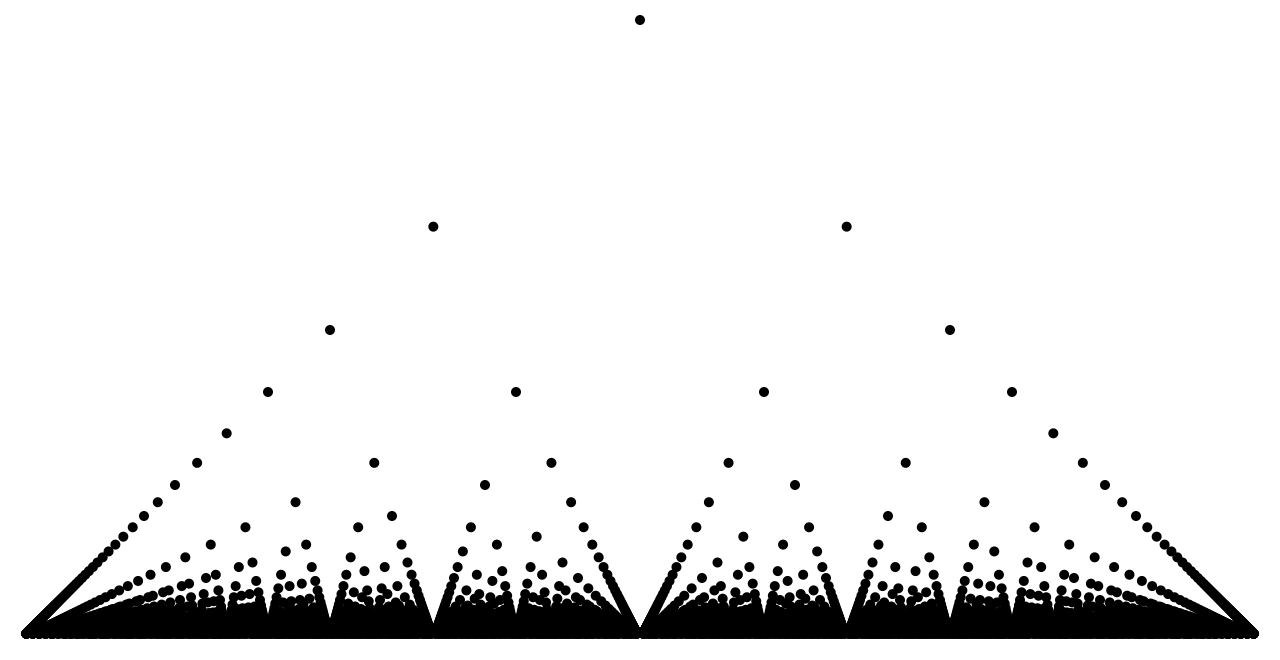
\includegraphics[width=6cm]{Thomae_function}
        \caption{Point plot of Thomae's function on $(0,1)$. The topmost point in the midle shows $f(\frac{1}{2}) = \frac{1}{2}$. Source: \href{https://en.wikipedia.org/wiki/Continuous_function}{Wikipedia{\tt/}continuous function}.}
    \end{figure}
\end{example}
In a similar vein,

\begin{example}
    \href{https://en.wikipedia.org/wiki/Dirichlet%27s_function}{Dirichlet's function}, the \href{https://en.wikipedia.org/wiki/Indicator_function}{indicator function} for the set of rational numbers,
    \begin{equation*}
        D(x) = \chi_{\mathbb{Q}} = \left\{\begin{split}
            &1&&\mbox{if } x\in\mathbb{Q},\\
            &0&&\mbox{if } x\in\mathbb{R}\backslash\mathbb{Q},
        \end{split}\right.
    \end{equation*}
    is nowhere continuous.
\end{example}

%------------------------------------------------------------------------------%

\subsubsection{Properties of continuous functions -- Tính chất của hàm liên tục}

\begin{lemma}
    Let $f(x)$ be a function that is continuous at a point $x_0$, \& $y_0$ be a value such that $f(x_0)\ne y_0$. Then $f(x)\ne y_0$ throughout some neighborhood of $x_0$.
\end{lemma}

\begin{bode}
    Cho $f(x)$ là hàm số liên tục tại điểm $x_0$, \& $y_0$ là giá trị sao cho $f(x_0)\ne y_0$. Khi đó $f(x)\ne y_0$ trong 1 vùng lân cận nào đó của $x_0$.
\end{bode}

\begin{proof}[Proof]
    By the definition of continuity, take $\varepsilon = \frac{1}{2}|y_0 - f(x_0)| > 0$, then there exists $\delta > 0$ s.t. $|f(x) - f(x_0)| < \frac{1}{2}|y_0 - f(x_0)|$ whenever $|x - x_0| < \delta$. Suppose there is a point in the neighborhood $|x - x_0| < \delta$ for which $f(x) = y_0$, then we have the contradiction $|y_0 - f(x_0)| < \frac{1}{2}|y_0 - f(x_0)|$.
    
    -- Theo định nghĩa về tính liên tục, lấy $\varepsilon = \frac{1}{2}|y_0 - f(x_0)| > 0$, khi đó tồn tại $\delta > 0$ s.t. $|f(x) - f(x_0)| < \frac{1}{2}|y_0 - f(x_0)|$ bất cứ khi nào $|x - x_0| < \delta$. Giả sử có 1 điểm trong lân cận $|x - x_0| < \delta$ sao cho $f(x) = y_0$, khi đó ta có mẫu thuẫn $|y_0 - f(x_0)| < \frac{1}{2}|y_0 - f(x_0)|$.
\end{proof}

%------------------------------------------------------------------------------%

\paragraph*{Intermediate value theorem.} The intermediate value theorem is an existence theorem, based on the real number property of completeness, \& states:

-- Định lý giá trị trung gian là 1 định lý tồn tại, dựa trên tính chất hoàn chỉnh của số thực, \& phát biểu:

\begin{theorem}[Intermediate value theorem]
    If the real-valued function $f$ is continuous on the closed interval $[a,b]$, \& $k$ is some number between $f(a)$ \& $f(b)$, then there is some number $c\in[a,b]$ s.t. $f(c) = k$.
\end{theorem}

\begin{dinhly}[Định lý giá trị trung gian]
    Nếu hàm số thực $f$ liên tục trên khoảng đóng $[a,b]$, \& $k$ là 1 số nào đó nằm giữa $f(a)$ \& $f(b)$, thì tồn tại 1 số $c\in[a,b]$ sao cho $f(c) = k$.
\end{dinhly}

\begin{corollary}
    If $f$ is continuous on $[a,b]$ \& $f(a),f(b)$ differ in sign, then, at some point $c\in[a,b]$, $f(c)$ must equal zero.
\end{corollary}

%------------------------------------------------------------------------------%

\paragraph*{Extreme value theorem -- Định lý giá trị cực đại.} The extreme value theorem states that if a function $f$ is defined on a closed interval $[a,b]$ (or any closed \& bounded set) \& is continuous there, then the function attains its maximum, i.e., there exists $c\in[a,b]$ with $f(c)\ge f(x)$, $\forall x\in[a,b]$. The same is true of the minimum of $f$. These statements are not, in general, true if the function is defined on an open interval $(a,b)$ (or any set that is not both closed \& bounded, i.e., compact), as, e.g., the continuous function $f(x) = \frac{1}{x}$, defined on the open interval $(0,1)$, does not attain a maximum, being unbounded above.

-- Định lý giá trị cực trị phát biểu rằng nếu 1 hàm $f$ được định nghĩa trên 1 khoảng đóng $[a,b]$ (hoặc bất kỳ tập đóng \& bị chặn nào) \& liên tục tại đó, thì hàm đạt giá trị cực đại của nó, tức là, tồn tại $c\in[a,b]$ với $f(c)\ge f(x)$, $\forall x\in[a,b]$. Điều tương tự cũng đúng với giá trị nhỏ nhất của $f$. Những phát biểu này, nói chung, không đúng nếu hàm được định nghĩa trên 1 khoảng mở $(a,b)$ (hoặc bất kỳ tập hợp nào không vừa đóng \& bị chặn, tức là compact), như, ví dụ, hàm liên tục $f(x) = \frac{1}{x}$, được định nghĩa trên khoảng mở $(0,1)$, không đạt giá trị cực đại, vì không bị chặn ở trên.

%------------------------------------------------------------------------------%

\paragraph*{Relation to differentiability \& integrability -- Quan hệ với sự khả vi \& sự khả tích.} Every differentiable function $f:(a,b)\to\mathbb{R}$ is continuous. The converse does not hold, e.g., the absolute value function
\begin{equation*}
    f(x) = |x| = \left\{\begin{split}
        &x&&\mbox{if } x\ge0,\\
        -&x&&\mbox{if } x < 0.
    \end{split}\right.
\end{equation*}
is everywhere continuous. However, it is not differentiable at $x = 0$ (but is so everywhere else). \href{https://en.wikipedia.org/wiki/Weierstrass_function}{Weierstrass's function} is also everywhere continuous but nowhere differentiable.

-- Mọi hàm khả vi $f:(a,b)\to\mathbb{R}$ đều liên tục. Điều ngược lại không đúng, ví dụ, hàm giá trị tuyệt đối
\begin{equation*}
    f(x) = |x| = \left\{\begin{split}
        &x&&\mbox{if } x\ge0,\\
        -&x&&\mbox{if } x < 0.
    \end{split}\right.
\end{equation*}
liên tục mọi nơi. Tuy nhiên, nó không khả vi tại $x = 0$ (nhưng khả vi tại mọi nơi khác). \href{https://en.wikipedia.org/wiki/Weierstrass_function}{Hàm Weierstrass} cũng liên tục mọi nơi nhưng không khả vi tại bất kỳ đâu.

The derivative $f'(x)$ of a differentiable function $f(x)$ need not be continuous. If $f'(x)$ be continuous, $f(x)$ is said to be {\it continuously differentiable}. The set of such functions is denoted $C^1((a,b))$. More generally, the set of functions $f:\Omega\to\mathbb{R}$ (from an open interval (or open subset of $\mathbb{R}$) $\Omega$ to the reals) s.t. $f$ is $n$ times differentiable \& s.t. the $n$th derivative of $f$ is continuous is denoted $C^n(\Omega)$. See \href{https://en.wikipedia.org/wiki/Smoothness#Differentiability_classes}{Wikipedia{\tt/}smoothness{\tt/}differentiabiity classes}. In the field of computer graphics, properties related (but not identical) to $C^0,C^1,C^2$ are sometimes called $G^0$ (continuity of position), $C^1$ (continuity of tangency), \& $G^2$ (continuity of curvature), see \href{https://en.wikipedia.org/wiki/Smoothness#Smoothness_of_curves_and_surfaces}{Wikipedia{\tt/}smoothness{\tt/}smoothness of curves \& surfaces}.

-- Đạo hàm $f'(x)$ của 1 hàm khả vi $f(x)$ không nhất thiết phải liên tục. Nếu $f'(x)$ liên tục, thì $f(x)$ được gọi là {\it khả vi liên tục}. Tập hợp các hàm như vậy được ký hiệu là $C^1((a,b))$. Tổng quát hơn, tập hợp các hàm $f:\Omega\to\mathbb{R}$ (từ 1 khoảng mở (hoặc tập con mở của $\mathbb{R}$) $\Omega$ đến các số thực) s.t. $f$ khả vi $n$ lần \& s.t. đạo hàm thứ $n$ của $f$ là liên tục được ký hiệu là $C^n(\Omega)$. Xem \href{https://en.wikipedia.org/wiki/Smoothness#Differentiability_classes}{Wikipedia{\tt/}smoothness{\tt/}differentiabiity classes}. Trong lĩnh vực đồ họa máy tính, các thuộc tính liên quan (nhưng không giống hệt) với $C^0,C^1,C^2$ đôi khi được gọi là $G^0$ (tính liên tục của vị trí), $C^1$ (tính liên tục của tiếp tuyến), \& $G^2$ (tính liên tục của độ cong), xem \href{https://en.wikipedia.org/wiki/Smoothness#Smoothness_of_curves_and_surfaces}{Wikipedia{\tt/}smoothness{\tt/}smoothness of curves \& surfaces}.

Every continuous function $f:[a,b]\to\mathbb{R}$ is \href{https://en.wikipedia.org/wiki/Integrable_function}{integrable} (e.g. in the sense of the \href{https://en.wikipedia.org/wiki/Riemann_integral}{Riemann integral}). The converse does not hold, as the (integrable but discontinuous) sign function ${\rm sgn}(x)$ shows.

-- Mọi hàm liên tục $f:[a,b]\to\mathbb{R}$ đều có thể tích phân (ví dụ theo nghĩa tích phân Riemann). Điều ngược lại không đúng, như hàm dấu ${\rm sgn}(x)$ (có thể khả tích nhưng không liên tục).

\paragraph*{Pointwise \& uniform limits -- Giới hạn điểm \& giới hạn đều.} Given a sequence $\{f_n\}_{n=1}^\infty$, $f_i:I\to\mathbb{R}$, $\forall i\in\mathbb{N}^\star$ of functions s.t. the limit $f(x)\coloneqq\lim_{n\to\infty} f_n(x)$ exists for all $x\in D$, the resulting function $f(x)$ is referred to as the \href{https://en.wikipedia.org/wiki/Pointwise_convergence}{pointwise limit} of the sequence of functions $\{f_n\}_{n\in\mathbb{N}^\star}$. The pointwise limit function need not be continuous, even if all functions $f_n$ are continuous. However, $f$ is continuous if all functions $f_n$ are continuous \& the sequence \href{https://en.wikipedia.org/wiki/Uniform_convergence}{converges uniformly}, by the \href{https://en.wikipedia.org/wiki/Uniform_convergence_theorem}{uniform convergence theorem}. This theorem can be used to show that the exponential functions, logarithms, square root function, \& trigonometric functions are continuous.

-- Cho 1 dãy hàm số $\{f_n\}_{n=1}^\infty$, $f_i:I\to\mathbb{R}$, $\forall i\in\mathbb{N}^\star$, tức là giới hạn $f(x)\coloneqq\lim_{n\to\infty} f_n(x)$ tồn tại với mọi $x\in D$, hàm số $f(x)$ kết quả được gọi là giới hạn từng điểm của dãy hàm số $\{f_n\}_{n\in\mathbb{N}^\star}$. Hàm giới hạn từng điểm không nhất thiết phải liên tục, ngay cả khi mọi hàm số $f_n$ đều liên tục. Tuy nhiên, $f$ là liên tục nếu mọi hàm số $f_n$ đều liên tục \& dãy số hội tụ đều, theo định lý hội tụ đều. Định lý này có thể được sử dụng để chứng minh rằng các hàm mũ, logarit, hàm căn bậc hai, \& hàm lượng giác là liên tục.

%------------------------------------------------------------------------------%

\subsubsection{Directional continuity -- Sự liên tục theo hướng}
Discontinuous functions may be discontinuous in a restricted way, giving rise to the concept of directional continuity (or right \& left continuous functions) \& semi-continuity. Roughly speaking, a function is {\it right-continuous} if no jump occurs when the limit point is approached from the right. 

\begin{definition}[Right-continuous function]
    A function $f$ is said to be {\rm right-continuous at a point} $c$ if the following holds: For any number $\varepsilon > 0$ however small, there exists some number $\delta > 0$ s.t. for all $x$ in the domain with $c < x < c + \delta$, the value of $f(x)$ will satisfy $|f(x) - f(c)| < \varepsilon$.
\end{definition}
This is the same condition as continuous functions, except it is required to hold for $x$ strictly larger than $c$ only. Requiring it instead for all $x$ with $c - \delta < x < c$ yields the notion of {\it left-continuous} functions. A function is continuous iff it is both right-continuous \& left-continuous.

-- Các hàm không liên tục có thể không liên tục theo một cách hạn chế, dẫn đến khái niệm về tính liên tục có hướng (hoặc các hàm liên tục phải \& trái) \& bán liên tục. Nói một cách đại khái, một hàm là {\it liên tục phải} nếu không xảy ra bước nhảy nào khi tiếp cận điểm giới hạn từ bên phải.

\begin{definition}[Hàm liên tục phải]
    Một hàm $f$ được gọi là {\rm liên tục phải tại một điểm} $c$ nếu điều sau đây đúng: Với mọi số $\varepsilon > 0$ dù nhỏ đến đâu, vẫn tồn tại một số $\delta > 0$ s.t. với mọi $x$ trong miền với $c < x < c + \delta$, giá trị của $f(x)$ sẽ thỏa mãn $|f(x) - f(c)| < \varepsilon$.
\end{definition}
Đây là điều kiện giống như các hàm liên tục, ngoại trừ việc nó chỉ đúng với $x$ lớn hơn $c$ một cách nghiêm ngặt. Yêu cầu nó thay thế cho mọi $x$ với $c - \delta < x < c$ tạo ra khái niệm về các hàm {\it liên tục trái}. Một hàm liên tục nếu và chỉ khi nó vừa liên tục phải \& liên tục trái.

%------------------------------------------------------------------------------%

\subsubsection{Semicontinuity -- Bán liên tục}
A function $f$ is {\it lower semi-continuous} if, roughly, any jumps that might occur only go down, but not up. I.e., for any $\varepsilon > 0$, there exists some number $\delta > 0$ s.t. for all $x$ in the domain with $|x - c| < \delta$, the value of $f(x)$ satisfies $f(x)\ge f(c) - \varepsilon$. The reverse condition is {\it upper semi-continuity}.

-- 1 hàm $f$ là {\it bán liên tục dưới} nếu, đại khái, bất kỳ bước nhảy nào có thể xảy ra chỉ đi xuống, nhưng không đi lên. Tức là, đối với bất kỳ $\varepsilon > 0$ nào, tồn tại một số $\delta > 0$ s.t. đối với mọi $x$ trong miền với $|x - c| < \delta$, giá trị của $f(x)$ thỏa mãn $f(x)\ge f(c) - \varepsilon$. Điều kiện ngược lại là {\it bán liên tục trên}.

%------------------------------------------------------------------------------%

\section{Continuous functions between metric spaces -- Các hàm liên tục giữa các không gian metric}

%------------------------------------------------------------------------------%

\section{Continuous functions between topological spaces -- Các hàm liên tục giữa các không gian tôpô}

%------------------------------------------------------------------------------%

\chapter{Series -- Chuỗi Số}
\minitoc

%------------------------------------------------------------------------------%

\section{Basic Series}
\textbf{\textsf{Resources -- Tài nguyên.}}
\begin{enumerate}
    \item \href{https://en.wikipedia.org/wiki/Series_(mathematics)}{Wikipedia{\tt/}series (mathematics)}.
\end{enumerate}




\begin{baitoan}[\cite{VMS_VMC2023}, 2.1, p. 32, VNUHCM UIT]
	Cho dãy số $\{x_n\}_{n=1}^\infty\subset(0,\infty)$ thỏa $\sum_{n=1}^\infty \dfrac{x_n}{(2n - 1)^2} < 1$. Chứng minh $\sum_{k=1}^\infty\sum_{n=1}^k \dfrac{x_n}{k^3} < 2$.
\end{baitoan}

\begin{baitoan}[\cite{VMS_VMC2023}, 2.2, p. 32, ĐHGTVT]
	Cho dãy số $\{a_n\}_{n=1}^\infty\subset(0,\infty)$ đặt bởi
	\begin{equation*}
		a_1 > 0,\ a_{n+1} = \frac{a_n^2}{a_n^2 - a_n + 1},\ \forall n\in\mathbb{N}^\star.
	\end{equation*}
	Tính $\sum_{n=1}^\infty a_n$.
\end{baitoan}

\begin{baitoan}[\cite{VMS_VMC2023}, 2.2, p. 32, ĐH Mỏ--Địa chất]
	Gọi $S$ là dãy con của dãy điều hòa $\left\{\dfrac{1}{n}\right\}_{n=1}^\infty = 1,\dfrac{1}{2},\dfrac{1}{3}\ldots,\dfrac{1}{n},\ldots$ \& có tổng hữu hạn. Gọi $c(n)$ là số lượng các phần tử của $S$ có số thứ tự trong dãy mẹ (điều hòa) ban đầu không vượt quá $n$. Chứng minh $\lim_{n\to\infty} \dfrac{c(n)}{n} = 0$.
\end{baitoan}

\begin{baitoan}[\cite{VMS_VMC2024}, p. 33, 2.1, ĐHCNTT TpHCM]
	Khảo sát sự hội tụ của chuỗi số
	\begin{equation*}
		\sum_{i=1}^{+\infty} \frac{\beta\sin^2l\alpha}{1 + \beta\sin^2k\alpha},\ \alpha\notin\{k\pi:k\in\mathbb{Z}\},\,\beta > 0.
	\end{equation*}
\end{baitoan}

%------------------------------------------------------------------------------%

\section{Fourier Series -- Chuỗi Fourier}

%------------------------------------------------------------------------------%

\chapter{Derivative \& Differentiability -- Đạo Hàm \& Tính Khả Vi}
\minitoc

%------------------------------------------------------------------------------%

\section{Định nghĩa đạo hàm. Ý nghĩa hình học của đạo hàm}
\textbf{\textsf{Resources -- Tài nguyên.}}
\begin{enumerate}
	\item \href{https://en.wikipedia.org/wiki/Derivative}{Wikipedia{\tt/}derivative}.
\end{enumerate}
In mathematics, the {\it derivative} is a fundamental tool that quantifies the sensitivity to change of a function's output w.r.t. its input. The derivative of a function of a single variable at a chosen input value, when it exists, is the \href{https://en.wikipedia.org/wiki/Slope}{slope} of the \href{https://en.wikipedia.org/wiki/Tangent}{tangent line} to the \href{https://en.wikipedia.org/wiki/Graph_of_a_function}{graph of the function} at that point. The tangent line is the best \href{https://en.wikipedia.org/wiki/Linear_approximation}{linear approximation} of the function near that input value. For this reason, the derivative is often described as the {\it instantaneous rate of change}, the ratio of the instantaneous change in the dependent variable to that of the independent variable. The process of finding a derivative is called {\it differentiation}.

-- Trong toán học, {\it đạo hàm} là 1 công cụ cơ bản định lượng độ nhạy với sự thay đổi của đầu ra của 1 hàm so với đầu vào của nó. Đạo hàm của 1 hàm của 1 biến duy nhất tại 1 giá trị đầu vào đã chọn, khi nó tồn tại, là độ dốc của đường tiếp tuyến với đồ thị của hàm tại điểm đó. Đường tiếp tuyến là phép xấp xỉ tuyến tính tốt nhất của hàm gần giá trị đầu vào đó. Vì lý do này, đạo hàm thường được mô tả là {\it tốc độ thay đổi tức thời}, tỷ lệ giữa sự thay đổi tức thời của biến phụ thuộc với biến độc lập. Quá trình tìm đạo hàm được gọi là {\it phép vi phân}.

There are multiple different notations for differentiation. \href{https://en.wikipedia.org/wiki/Leibniz_notation}{Leibniz notation}, named after \href{https://en.wikipedia.org/wiki/Gottfried_Wilhelm_Leibniz}{\sc Gottfried Wilhelm Leibniz}, is represented as the ratio of 2 \href{https://en.wikipedia.org/wiki/Differential_(mathematics)}{differentials}, whereas {\it prime notation} is written by adding a prime mark. Higher order notations represent repeated differentiation, \& they are usually denoted in Leibniz notation by adding superscripts to the differentials, \& in prime notation by adding additional prime marks. The \href{https://en.wikipedia.org/wiki/Higher_order_derivative}{higher order derivatives} can be applied in physics, e.g., while the 1st derivative of the position of a moving object w.r.t. time is the object's \href{https://en.wikipedia.org/wiki/Velocity}{velocity}, how the position changes as time advances, the 2nd derivative is the object's \href{https://en.wikipedia.org/wiki/Acceleration}{acceleration}, how the velocity changes as time advances.

-- Có nhiều ký hiệu khác nhau cho phép tính vi phân. Ký hiệu Leibniz, được đặt theo tên của Gottfried Wilhelm Leibniz, được biểu diễn dưới dạng tỷ số của hai phép tính vi phân, trong khi ký hiệu nguyên tố được viết bằng cách thêm 1 dấu nguyên tố. Ký hiệu bậc cao hơn biểu diễn phép tính vi phân lặp lại và chúng thường được biểu diễn trong ký hiệu Leibniz bằng cách thêm các chữ số mũ vào các phép tính vi phân, và trong ký hiệu nguyên tố bằng cách thêm các dấu nguyên tố bổ sung. Các đạo hàm bậc cao hơn có thể được áp dụng trong vật lý; ví dụ, trong khi đạo hàm bậc nhất của vị trí của 1 vật chuyển động theo thời gian là vận tốc của vật, cách vị trí thay đổi khi thời gian trôi qua, thì đạo hàm bậc hai là gia tốc của vật, cách vận tốc thay đổi khi thời gian trôi qua.

Derivatives can be generalized to \href{https://en.wikipedia.org/wiki/Function_of_several_real_variables}{functions of several real variables}. In this case, the derivative is reinterpreted as a \href{https://en.wikipedia.org/wiki/Linear_transformation}{linear transformation} whose graph is (after an appropriate translation) the best linear approximation to the graph of the original function. The \href{https://en.wikipedia.org/wiki/Jacobian_matrix}{Jacobian matrix} is the matrix that represents this linear transformation w.r.t. the basis given by the choice of independent \& dependent variables. It can be calculated in terms of the \href{https://en.wikipedia.org/wiki/Partial_derivative}{partial derivatives} w.r.t. the independent variables. For a \href{https://en.wikipedia.org/wiki/Real-valued_function}{real-valued function} of several variables, the Jacobian matrix reduces to the \href{https://en.wikipedia.org/wiki/Gradient_vector}{gradient vector}.

Nếu quỹ đạo chuyển động của 1 vật hay 1 chất điểm được miêu tả bằng hàm số ${\bf x}(t)$ theo thời gian thì vận tốc ${\bf v}(t) = {\bf x}'(t)$ biểu thị độ nhanh chậm của chuyển động tại 1 thời điểm $t$.

%------------------------------------------------------------------------------%

\subsection{Definition of derivative as a limit -- Định nghĩa đạo hàm như 1 giới hạn}

\begin{definition}[$\varepsilon$-$\delta$ definition of derivative]
	A \href{https://en.wikipedia.org/wiki/Function_of_a_real_variable}{function of a real variable} $f(x)$ is \href{https://en.wikipedia.org/wiki/Differentiable_function}{differentiable} at a point $a$ of its domain, if its domain contains an open interval containing $a$, \& the limit
	\begin{equation*}
		l = \lim_{h\to0} \frac{f(a + h) - f(a)}{h}
	\end{equation*}
	exists. I.e., for every positive real number $\varepsilon\in(0,\infty)$, there exists a positive real number $\delta = \delta(\varepsilon)\in(0,\infty)$ s.t., for every $h\ne0$ s.t. $|h| < \delta$ then $f(a + h)$ is defined, \&
	\begin{equation*}
		\left|\frac{f(a + h) - f(a)}{h} - l\right| < \varepsilon.
	\end{equation*}
\end{definition}
If the function $f$ is differentiable at $a$, i.e., if the limit $l$ exists, then this limit is called the {\it derivative} of $f$ at $a$. Multiple notations for the derivative exist. The derivative of $f$ at $a$ can be denoted $f'(a)$, read as ``$f$ prime of $a$''; or it can be denoted $\frac{df}{dx}(a)$, read as ``the derivative of $f$ w.r.t. $x$ at $a$'' or ``$df$ by (or over) $dx$ at $a$''. If $f$ is a function that has a derivative at every point in its domain, then a function can be defined by mapping every point $x$ to the value of the derivative of $f$ at $x$. This function is written $f'$ \& is called the {\it derivative function} or the {\it derivative of $f$}. The function $f$ sometimes has a derivative at most, but not all, points of its domain. The function whose value at $a$ equals $f'(a)$ whenever $f'(a)$ is defined \& elsewhere is undefined is also called the derivative of $f$. It is still a function, but its domain may be smaller than the domain of $f$.

-- Nếu hàm $f$ khả vi tại $a$, tức là nếu giới hạn $l$ tồn tại, thì giới hạn này được gọi là {\it đạo hàm} của $f$ tại $a$. Có nhiều ký hiệu cho đạo hàm. Đạo hàm của $f$ tại $a$ có thể được ký hiệu là $f'(a)$, đọc là ``$f$ phẩy của $a$''; hoặc có thể được ký hiệu là $\frac{df}{dx}(a)$, đọc là ``đạo hàm của $f$ theo $x$ tại $a$'' hoặc ``$df$ theo (hoặc trên) $dx$ tại $a$''. Nếu $f$ là hàm có đạo hàm tại mọi điểm trong tập xác định của nó, thì hàm có thể được định nghĩa bằng cách ánh xạ mọi điểm $x$ tới giá trị của đạo hàm của $f$ tại $x$. Hàm này được ký hiệu là $f'$ \& được gọi là {\it đạo hàm hàm} hoặc {\it đạo hàm của $f$}. Hàm $f$ đôi khi có đạo hàm tại nhiều nhất, nhưng không phải tất cả, các điểm của tập xác định của nó. Hàm có giá trị tại $a$ bằng $f'(a)$ bất cứ khi nào $f'(a)$ được xác định \& ở nơi khác không xác định cũng được gọi là đạo hàm của $f$. Nó vẫn là 1 hàm, nhưng tập xác định của nó có thể nhỏ hơn tập xác định của $f$.

The ratio in the definition of the derivative is the slope of the line through 2 points on the graph of the function $f$, specially the points $(a,f(a))$ \& $(a + h,f(a + h))$. As $h$ is made smaller, these points grow closer together, \& the slope of this line approaches the limiting value, the slope of the tangent to the graph of $f$ at $a$. I.e., the derivative is the slope of the tangent.

-- Tỷ lệ trong định nghĩa của đạo hàm là độ dốc của đường thẳng qua 2 điểm trên đồ thị của hàm số $f$, đặc biệt là các điểm $(a,f(a))$ \& $(a + h,f(a + h))$. Khi $h$ nhỏ hơn, các điểm này sẽ gần nhau hơn, \& độ dốc của đường thẳng này tiến tới giá trị giới hạn, độ dốc của tiếp tuyến với đồ thị của $f$ tại $a$. I.e., đạo hàm là độ dốc của tiếp tuyến.

%------------------------------------------------------------------------------%

\subsubsection{Definition of derivative using infinitesimals -- Định nghĩa đạo hàm sử dụng vô cùng nhỏ}
1 way to think of the derivative $\frac{df}{dx}(a)$ is as the ratio of an \href{https://en.wikipedia.org/wiki/Infinitesimal}{infinitesimal} change in the output of the function $f$ to an infinitesimal change in its input. In order to make this intuition rigorous, a system of rules for manipulating infinitesimal quantities is required. The system of \href{https://en.wikipedia.org/wiki/Hyperreal_number}{hyperreal numbers} is a way of treating infinite \& infinitesimal quantities. The hyperreals are an \href{https://en.wikipedia.org/wiki/Field_extension}{extension} of the real numbers that contain numbers greater than anything of the form $1 + 1 + \cdots + 1$ for any finite number of terms. Such numbers are infinite, \& their \href{https://en.wikipedia.org/wiki/Multiplicative_inverse}{reciprocals} are infinitesimals. The application if hyperreal numbers to the foundations of calculus is called \href{https://en.wikipedia.org/wiki/Nonstandard_analysis}{nonstandard analysis}. This provides a way to define the basic concepts of calculus such as the derivative \& integral in terms of infinitesimals, thereby giving a precise meaning to the $d$ in the Leibniz notation. Thus, the derivative of $f(x)$ becomes
\begin{equation*}
	f'(x) = {\rm st}\left(\frac{f(x + dx) - f(x)}{dx}\right)
\end{equation*}
for an arbitrary infinitesimal $dx$, where st denotes the \href{https://en.wikipedia.org/wiki/Standard_part_function}{standard part function}, which ``rounds off'' each finite hyperreal to the nearest real.

%------------------------------------------------------------------------------%

\subsection{Continuity \& differentiability -- Liên tục \& khả vi}
If $f$ is differentiable at $a$, then $f$ must also be continuous at $a$. E.g., choose a point $a$ \& let $f$ be the \href{https://en.wikipedia.org/wiki/Step_function}{step function}
\begin{equation*}
	{\rm step}(x;a,a_l,a_r) = \left\{\begin{split}
		&a_l&&\mbox{if } x < a,\\
		&a_r&&\mbox{if } x\ge a.
	\end{split}\right.\mbox{ for }a\in\mathbb{R},a_l,a_r\in\mathbb{C},a_l\ne a_r.
\end{equation*}

\begin{remark}
	This step function is very common in the mathematical analysis of hyperbolic Partial Differential Equations (abbr., hyperbolic PDEs), especially in the shock waves \& rarefaction waves -- solutions of Riemann problem.
	
	-- Hàm bước này rất phổ biến trong phân tích toán học của Phương trình đạo hàm riêng hypebolic (viết tắt là PDE hypebolic), đặc biệt là trong sóng xung kích \& sóng loãng -- các nghiệm của bài toán Riemann.
\end{remark}
The function ${\rm step}(x;a,a_l,a_r)$ cannot have a derivative at $a$. If $h < 0$, then $a + h$ is on the low part of the step, so the secant line from $a$ to $a + h$ is very steep; as $h$ tends to 0, the slope tends to $\infty$. If $h > 0$, then $a + h$ is on the high part of the step, so the secant line from $a$ to $a + h$ has slope 0. Consequently, the secant lines do not approach any single slope, so the limit of the difference quotient does not exist. However, even if a function is continuous at a point, it may not be differentiable there.

-- Hàm ${\rm step}(x;a,a_l,a_r)$ không thể có đạo hàm tại $a$. Nếu $h < 0$, thì $a + h$ nằm ở phần thấp của bậc, do đó đường cắt từ $a$ đến $a + h$ rất dốc; khi $h$ tiến tới 0, độ dốc tiến tới $\infty$. Nếu $h > 0$, thì $a + h$ nằm ở phần cao của bậc, do đó đường cắt từ $a$ đến $a + h$ có độ dốc 0. Do đó, các đường cắt không tiến tới bất kỳ độ dốc đơn nào, do đó giới hạn của thương hiệu không tồn tại. Tuy nhiên, ngay cả khi 1 hàm liên tục tại 1 điểm, thì nó có thể không khả vi tại đó.

\begin{problem}
	Prove that the \href{https://en.wikipedia.org/wiki/Absolute_value}{absolute value} function given by $f(x) = |x|$ is continuous at $x = 0$, but it is not differentiable there.
\end{problem}

\begin{proof}
	If $h > 0$, then the slope of the secant line from 0 to $h$ is 1. If $h < 0$, then the slope of the secant line from 0 to $h$ is $-1$. This can be seen graphically as a ``kink'' or a ``cusp'' in the graph at $x = 0$.
\end{proof}

\begin{problem}
	Investigate the continuity \& differentiability of functions: (a) $x^a|x|$, $a > 0$. (b) $x^a|x|$, $a < 0$. (c) $x^a|x|^b$ for $a,b\in\mathbb{R}$.
\end{problem}
Even a function with a smooth graph is not differentiable at a point where its \href{https://en.wikipedia.org/wiki/Vertical_tangent}{tangent is vertical}, e.g.:

-- Ngay cả 1 hàm số có đồ thị trơn cũng không khả vi tại điểm mà tiếp tuyến của nó thẳng đứng, e.g.:

\begin{problem}
	Prove that the function $f(x) = x^{\frac{1}{3}} = \sqrt[3]{x}$ is continuous on the whole $\mathbb{R}$ but not differentiable at $x = 0$.
\end{problem}
In summary, a function that has a derivative is continuous, but there are continuous functions that do not have a derivative.

-- Tóm lại, 1 hàm số có đạo hàm là hàm số liên tục, nhưng có những hàm số liên tục nhưng không có đạo hàm.

Most functions that occur in practice have derivatives at all points or \href{https://en.wikipedia.org/wiki/Almost_everywhere}{almost every} point. Early in the \href{https://en.wikipedia.org/wiki/History_of_calculus}{history of calculus}, many mathematicians assumed that a continuous function was differentiable at most points. Under mild conditions (e.g., if the function is a \href{https://en.wikipedia.org/wiki/Monotone_function}{monotone} or a \href{https://en.wikipedia.org/wiki/Lipschitz_function}{Lipschitz function}), this is true. However, in 1872, {\sc Weierstrass} found the 1st example of a function, called the \href{https://en.wikipedia.org/wiki/Weierstrass_function}{Weierstrass function}, that is continuous everywhere but differentiable nowhere. In 1931, \href{https://en.wikipedia.org/wiki/Stefan_Banach}{\sc Stefan Banach} proved that the set of functions that have a derivative at some point is a \href{https://en.wikipedia.org/wiki/Meager_set}{meager set} in the space of all continuous functions. Informally, this means that hardly any random continuous functions have a derivative at even 1 point.

-- Hầu hết các hàm xuất hiện trong thực tế đều có đạo hàm tại mọi điểm hoặc hầu như mọi điểm. Vào đầu lịch sử phép tính, nhiều nhà toán học cho rằng 1 hàm liên tục có thể vi phân tại hầu hết các điểm. Trong điều kiện nhẹ nhàng (ví dụ, nếu hàm là hàm đơn điệu hoặc hàm Lipschitz), điều này là đúng. Tuy nhiên, vào năm 1872, {\sc Weierstrass} đã tìm thấy ví dụ đầu tiên về 1 hàm, được gọi là hàm Weierstrass, liên tục ở mọi nơi nhưng không thể vi phân ở bất kỳ đâu. Vào năm 1931, {\sc Stefan Banach} đã chứng minh rằng tập hợp các hàm có đạo hàm tại 1 điểm nào đó là 1 tập hợp ít ỏi trong không gian của tất cả các hàm liên tục. Nói 1 cách không chính thức, điều này có nghĩa là hầu như không có hàm liên tục ngẫu nhiên nào có đạo hàm tại 1 điểm.

%------------------------------------------------------------------------------%

\subsection{Notation for differentiation -- Ký hiệu cho phép lấy đạo hàm}
\textbf{\textsf{Resources -- Tài nguyên.}}
\begin{enumerate}
	\item \href{https://en.wikipedia.org/wiki/Notation_for_differentiation}{Wikipedia{\tt/}notation for differentiation}.
\end{enumerate}
1 common way of writing the derivative of a function is \href{https://en.wikipedia.org/wiki/Leibniz_notation}{Leibniz notation}, introduced by \href{https://en.wikipedia.org/wiki/Gottfried_Leibniz}{\sc Gottfried Wilhelm Leibniz} in 1675, which denotes a derivative as the quotient of 2 \href{https://en.wikipedia.org/wiki/Differential_(mathematics)}{differentials} e.g. $dx,dy$. It is still common used when the equation $y = f(x)$ is viewed as a functional relationship between \href{https://en.wikipedia.org/wiki/Dependent_and_independent_variables}{dependent \& independent variables}. The 1st derivative is denoted by $\frac{dy}{dx}$, read as ``the derivative of $y$ w.r.t. $x$''. This derivative can alternately be treated as the application of a \href{https://en.wikipedia.org/wiki/Differential_operator}{differential operator} to a function, $\frac{dy}{dx} = \frac{d}{dx}f(x)$. Higher derivatives are expressed using the notation $\frac{d^ny}{dx^n}$ for the $n$th derivative of $y = f(x)$. These are abbreviations for multiple applications of the 

%------------------------------------------------------------------------------%

\section{L'H\^ospital's rule -- Quy tắc l'H\^ospital}
\textbf{\textsf{Resources -- Tài nguyên.}}
\begin{enumerate}
	\item \href{https://en.wikipedia.org/wiki/L%27H%C3%B4pital%27s_rule}{Wikipedia{\tt/}L'H\^ospital rule}.
	\item \cite{Rudin1976}. {\sc Walter Rudin}. {\it Principles of Mathematical Analysis}. Sect: L'Hospital's rule, pp. 109--110.
	\item \cite{Tao_analysis_1}. {\sc Terence Tao}. {\it Analysis I}. Sect. 10.5: L'H\^ospital's Rule, pp. 228--229.
\end{enumerate}
{\it L'Hôpital's rule}, also known as {\it Bernoulli's rule}. is a mathematical theorem that allows evaluating limits of \href{https://en.wikipedia.org/wiki/Indeterminate_form}{indeterminate forms} using derivatives. Application (or repeated application) of the rule often converts an indeterminate form to an expression that can be easily evaluated by substitution. The rule is named after the 17th-century French mathematician \href{https://en.wikipedia.org/wiki/Guillaume_de_l%27H%C3%B4pital}{Guillaume de l'H\^opital}. Although the rule is often attributed to de l''H\^opital, the theorem was 1st introduced to him in 1694 by the Swiss mathematician \href{https://en.wikipedia.org/wiki/Johann_Bernoulli}{\sc Johann Bernoulli}.

The following theorem is frequently useful in the evaluation of limits. The differentiation of the numerator \& denominator often simplifies the quotient or converts it to a limit that can be directly evaluated by \href{https://en.wikipedia.org/wiki/Continuous_function}{continuity}.

\begin{theorem}[\cite{Rudin1976}, Thm. 5.13, p. 109, l'H\^ospital's rule]
	\label{thm: l'H\^ospital rule}
	suppose $f,g$ are real \& differentiable in $(a,b)$, \& $g'(x)\ne0$, $\forall x\in(a,b)$, where $-\infty\le a < b\le\infty$. Suppose $\frac{f'(x)}{g'(x)}\to l$ as $x\to a$. If $f(x)\to0$ \& $g(x)\to0$ as $x\to a$, or if $g(x)\to\infty$ as $x\to a$, then $\frac{f(x)}{g(x)}\to l$ as $x\to a$. The analogous statement is also true if $x\to b$, or if $g(x)\to-\infty$ instead of $g(x)\to\infty$.
\end{theorem}

\begin{theorem}[\cite{Tao_analysis_1}, Prop. 10.5.1, p. 228, L'H\^ospital's rule I]
	Let $X\subset\mathbb{R}$, let $f:X\to\mathbb{R},g:X\to\mathbb{R}$ be functions, \& let $x_0\in X$ be a limit point of $X$. Suppose that $f(x_0) = g(x_0) = 0$, that $f,g$ are both differentiable at $x_0$, but $g'(x_0)\ne0$. Then there exists a $\delta > 0$ such that $g(x)\ne0$, $\forall x\in(X\cap(x_0 - \delta,x_0 + \delta))\backslash\{x_0\}$, \&
	\begin{equation*}
		\lim_{x\to x_0,\ x\in(X\cap(x_0 - \delta,x_0 + \delta))\backslash\{x_0\}} \frac{f(x)}{g(x)} = \frac{f'(x_0)}{g'(x_0)}.
	\end{equation*}
\end{theorem}

\begin{baitoan}
	Cho hàm số $f(x) = \sin x,g(x) = -\frac{1}{2}x$. Chứng minh hàm số
	\begin{equation*}
		h(x)\coloneqq\left\{\begin{split}
			&\frac{f(x)}{g(x)}&&\mbox{if } x\ne0,\\
			&\frac{f'(0)}{g'(0)} = -2&&\mbox{if } x = 0.
		\end{split}\right.\in C(\mathbb{R}).
	\end{equation*}
\end{baitoan}

\begin{problem}
	Suppose $f,g$ are complex differentiable functions on $(0,1)$, $f(x)\to0,g(x)\to0,f'(x)\to A,g'(x)\to B$ as $x\to0$, where $A,B\in\mathbb{C}$, $B\ne0$. Prove that $\lim_{x\to0} \frac{f(x)}{g(x)} = \frac{A}{B}$.
\end{problem}
{\sf Hint.} $\frac{f(x)}{g(x)} = \left(\frac{f(x)}{x} - A\right)\frac{x}{g(x)} + A\frac{x}{g(x)}$ then apply l'H\^ospital rule, i.e., Thm. \ref{thm: l'H\^ospital rule} to the real- \& imaginary parts of $\frac{f(x)}{x},\frac{g(x)}{x}$.

%------------------------------------------------------------------------------%

\subsection{Problems: Derivative -- Bài tập: Đạo hàm}

\begin{baitoan}
	Tính đạo hàm bằng định nghĩa $\forall x_0\in\mathbb{C}$: (a) $(x)'|_{x=x_0}$. (b) $(x^2)'|_{x=x_0}$. (c) $(x^n)'|_{x=x_0}$, $\forall n\in\mathbb{N}$. (d) $(x^{-n})'|_{x=x_0}$, $\forall n\in\mathbb{N}$. (e) $(\sqrt{x})'|_{x=x_0}$. (f) $(\sqrt[3]{x})'|_{x=x_0}$. (g) $(\sqrt[n]{x})'|_{x=x_0}$, $\forall n\in\mathbb{N}$. (h) $(\sqrt[n]{x^m})|_{x=x_0}$, $\forall m,n\in\mathbb{N}$. (i) $(x^a)'|_{x=x_0}$, $\forall a\in\mathbb{R}$.
\end{baitoan}

\begin{baitoan}[Derivative of polynomials -- Đạo hàm của các đa thức]
	Tính đạo hàm của hàm số đa thức
	\begin{equation}
		\label{polynomial}
		\tag{P}
		P(x;n,{\bf a})\coloneqq\sum_{i=0}^n a_ix^i = a_nx^n + a_{n-1}x^{n-1} + \cdots + a_1x + a_0,
	\end{equation}
	tại $x = x_0$ bằng định nghĩa, với $\deg P(x;n,{\bf a}) = n\in\mathbb{N}$ \& vector chứa các hệ số của đa thức $P(x;n,{\bf a})$ là ${\bf a}\coloneqq(a_0,a_1,\ldots,a_n)\in\mathbb{R}^n\times\mathbb{R}^\star$.
\end{baitoan}

\begin{baitoan}[Derivative of rational function -- Đạo hàm của phân thức]
	Tính đạo hàm của hàm số phân thức
	\begin{equation}
		\label{rational function}
		\tag{Q}
		Q(x;m,n,{\bf a},{\bf b})\coloneqq\frac{\sum_{i=0}^m a_ix^i}{\sum_{i=0}^n b_ix^i} = \frac{a_mx^m + a_{m-1}x^{m-1} + \cdots + a_1x + a_0}{b_nx^n + b_{n-1}x^{n-1} + \cdots + b_1x + b_0},
	\end{equation}
	tại $x = x_0$ bằng định nghĩa.
\end{baitoan}

\begin{baitoan}[Đạo hàm của căn thức]
	Tính đạo hàm của hàm số căn thức $f(x) = \sqrt[n]{x} = x^{\frac{1}{n}}$, với $n\in\mathbb{N}^\star$, tại $x = x_0$ bằng định nghĩa.
\end{baitoan}
Ta có 3 dạng hàm số sơ cấp thường gặp: hàm đa thức $P(x;n,{\bf a})\coloneqq\sum_{i=0}^n a_ix^i$, hàm phân thức $Q(x;m,n,{\bf a},{\bf b})\coloneqq\dfrac{\sum_{i=0}^m a_ix^i}{\sum_{i=0}^n b_ix^i}$, hàm căn thức $R_n(x)\coloneqq\sqrt[n]{x}$.

\begin{baitoan}[\cite{TLCT_BT_dai_so_giai_tich_11}, 1., p. 49]
	Dùng định nghĩa, tính đạo hàm của hàm số tại điểm $x_0$: (a) $y = 2x + 1,x_0 = 2$. (b) $y = x^2 + 3x,x_0 = 1$. (c) $y = ax + b$ tại $x = x_0$. (d) $y = ax^2 + bx + c$ tại $x = x_0$.
\end{baitoan}

\begin{baitoan}[\cite{TLCT_BT_dai_so_giai_tich_11}, 2., p. 49]
	Cho parabol $y = x^2$ \& 2 điểm $A(2,4),B(2 + \Delta x,4 + \Delta y)$ trên parabol đó. (a) Tính hệ số góc của cát tuyến $AB$ biết $\Delta x\in\{1,0.1,0.01\}$. (b) Tính hệ số góc của tiếp tuyến của parabol đã cho tại điểm $A$. (c) Mở rộng cho parabol $y = ax^2 + bx + c$ \& 2 điểm $A(x_0,y_0),B(x_0 + \Delta x,y_0 + \Delta y)$.
\end{baitoan}

\begin{baitoan}[\cite{TLCT_BT_dai_so_giai_tich_11}, 3., p. 49]
	Viết phương trình tiếp tuyến của đồ thị hàm số $y = x^3$ biết: (a) Tiếp tuyến có hoành độ bằng $1$. (b) Tiếp điểm của tung độ bằng $8$. (c) Hệ số góc của tiếp tuyến bằng $3$.
\end{baitoan}

\begin{baitoan}[\cite{TLCT_BT_dai_so_giai_tich_11}, 4., p. 49]
	1 vật rơi tự do có phương trình chuyển động $S = \frac{gt^2}{2}$ với $g\approx9.8{\rm m{\tt/}s^2}$ \& $t$ (s). Tính: (a) Vận tốc trung bình trong khoảng thời gian từ $t$ đến $t + \Delta t$ với độ chính xác $0.001$, biết $t = 5$ \& $\Delta t\in\{0.1,0.001,0.001\}$. (b) Vận tốc tại thời điểm $t = 5$.
\end{baitoan}

\begin{baitoan}[\cite{TLCT_BT_dai_so_giai_tich_11}, 5., p. 49]
	Tính đạo hàm của hàm số $y = \sqrt[3]{x}$ trên $(0,\infty)$.
\end{baitoan}

\begin{baitoan}[\cite{TLCT_BT_dai_so_giai_tich_11}, 6., p. 49]
	Tính đạo hàm của hàm số $y = x|x|$ tại điểm $x_0 = 0$ (nếu có).
\end{baitoan}

\begin{baitoan}[\cite{TLCT_BT_dai_so_giai_tich_11}, 7., p. 49]
	Tính $f'(x)$ với
	\begin{equation}
		f(x) = \left\{\begin{split}
			&2x + 1&&\mbox{if } x < 1,\\
			&x^2 + 2&&\mbox{if } 1\le x\le2,\\
			&x^3 - x^2 - 8x + 10&&\mbox{if } x > 2.
		\end{split}\right.
	\end{equation}
\end{baitoan}

%------------------------------------------------------------------------------%

\section{Differentiation Rules -- Các Quy Tắc Tính Đạo Hàm}

\begin{baitoan}[\cite{TLCT_BT_dai_so_giai_tich_11}, 8., p. 50]
	Tính đạo hàm của hàm số: (a) $y = x^4 - 3x^3 + 5x^2 - 7x + 9$. (b) $y = (x - 1)^5(x + 1)^7$. (c) $y = \dfrac{x^2 + 1}{x^4 + 1}$. (d) $y = (x + 1)^3(x + 2)^4(x + 3)^5$.
\end{baitoan}

\begin{baitoan}[\cite{TLCT_BT_dai_so_giai_tich_11}, 9., p. 50]
	Tính đạo hàm của hàm số: (a) $y = \sqrt{\dfrac{1 - x}{1 + x}}$. (b) $y = \sin x^2 + x\cos x^2$. (c) $y = \ln(x + \sqrt{x^2 + 1})$. (d) $y = (x^3 + x^2 + x + 1)e^{x^2 + x}$.
\end{baitoan}

\begin{baitoan}[\cite{TLCT_BT_dai_so_giai_tich_11}, 10., p. 50]
	Tính đạo hàm của hàm số: (a) $y = \dfrac{\sin x - \cos x}{\sin x + \cos x}$. (b) $y = \dfrac{\sin x - 1}{\sin x + \cos x}$.
\end{baitoan}

\begin{baitoan}[\cite{TLCT_BT_dai_so_giai_tich_11}, 11., p. 50]
	Viết phương trình tiếp tuyến của đồ thị hàm số: (a) $y = \dfrac{x}{x^2 + 1}$ biết hoành độ tiếp điểm là $x_0 = \frac{1}{2}$. (b) $y = \sqrt{x + 2}$ biết tung độ tiếp điểm là $y_0 = 2$.
\end{baitoan}

\begin{baitoan}[\cite{TLCT_BT_dai_so_giai_tich_11}, 12., p. 50]
	(a) Chứng minh hàm số $y = f(x) = \sin^6x + \cos^6x + 3\sin^2x\cos^2x$ có đạo hàm bằng $0$. (b) Mở rộng bài toán.
\end{baitoan}

\begin{proof}
    (a) $y = f(x) = \sin^6x + \cos^6x + 3\sin^2x\cos^2x = \sin^6x + \cos^6x + 3\sin^2x\cos^2x(\sin^2x + \cos^2x) = (\sin^2x + \cos^2x)^3 = 1\Rightarrow f'(x) = 0$, $\forall x\in\mathbb{R}$. (b) Xét hàm $f:D_f\subset\mathbb{R}\to\mathbb{R}$ bất kỳ sao cho $1\in D_f$ \& $f$ khả vi tại $x = 1$. Đặt $g(x)\coloneqq\sin^2x + \cos^2x\equiv1$, thì $g'(x) = 1' = 0$ (hoặc tính cụ thể $g'(x) = 2\sin x\cos x - 2\cos x\sin x = 0$), $\forall x\in\mathbb{R}$. Khi đó đạo hàm của hàm hợp $f\circ g$ sẽ bằng $0$ vì $(f\circ g)'(x) = (f(1))' = 0$, hoặc theo quy tắc xích $(f\circ g)'(x) = f'(g(x))g'(x) = f'(1)\cdot0 = 0$.
\end{proof}

\begin{remark}
    Mấu chốt của bài toán chỉ là dùng đẳng thức lượng giác cơ bản $\sin^2x + \cos^2x = 1$, $\forall x\in\mathbb{R}$, để đưa về đạo hàm của hàm hằng bằng $0$. Tương tự nếu ta có 1 đẳng thức đại số hoặc 1 đẳng thức lượng giác nói riêng, hoặc 1 đẳng thức toán học có dạng $g(x) = a\in\mathbb{R}$. Xét hàm $f:D_f\subset\mathbb{R}\to\mathbb{R}$ bất kỳ sao cho $a\in D_f$ \& $f$ khả vi tại $x = a$. Khi đó đạo hàm của hàm hợp $f\circ g$ sẽ bằng $0$ vì $(f\circ g)'(x) = (f(a))' = 0$, hoặc theo quy tắc xích $(f\circ g)'(x) = f'(g(x))g'(x) = f'(a)(a)' = f'(a)\cdot0 = 0$, $\forall x\in\mathbb{R}$.
\end{remark}

\begin{baitoan}[\cite{TLCT_BT_dai_so_giai_tich_11}, 13., p. 50]
	Viết phương trình tiếp tuyến của parabol $y = x^2$ biết tiếp tuyến đó đi qua điểm $A(0,-1)$.
\end{baitoan}

\begin{baitoan}[\cite{TLCT_BT_dai_so_giai_tich_11}, 14., p. 50]
	1 viên đạn được bắn lên từ mặt đất theo phương thẳng đứng với tốc độ ban đầu $v_0 = 196$ {\rm m{\tt/}s} (bỏ qua sức cản của không khí). Tìm thời điểm tại đó tốc độ của viên đạn bằng $0$. Khi đó viên đạn cách mặt đất bao nhiêu {\rm m}?
\end{baitoan}

%------------------------------------------------------------------------------%

\section{Numerical Differentiation -- Xấp Xỉ Đạo Hàm}
\textbf{\textsf{Resources -- Tài nguyên.}}
\begin{enumerate}
	\item \href{https://en.wikipedia.org/wiki/Numerical_differentiation}{Wikipedia{\tt/}numerical differentiation}.
    
	\item \cite{Scheid1989}. {\sc Francis Scheid}. {\it Schaum's Outline of Numerical Analysis}. Chap. 13: Numerical Differentiation.
    
	\item \cite{LeVeque2007}. {\sc Randall J. LeVeque}. {\it Finite Difference Methods for Ordinary \& Partial Differential Equations: Steady-State \& Time-Dependent Problems}.
\end{enumerate}
In \href{https://en.wikipedia.org/wiki/Numerical_analysis}{numerical analysis}, {\it numerical differentiation} algorithms estimate the derivative of a mathematical function or \href{https://en.wikipedia.org/wiki/Function_(computer_programming)}{subroutine} using values of the function \& perhaps other knowledge about the function.

-- Trong phân tích số, thuật toán phân biệt số ước tính đạo hàm của 1 hàm toán học hoặc chương trình con bằng cách sử dụng các giá trị của hàm \& có thể là các kiến thức khác về hàm.

%------------------------------------------------------------------------------%

\subsection{Approximate 1st-order derivatives -- Xấp xỉ đạo hàm bậc nhất}
Approximate derivatives of a function $y = f(x)$ may be found from a polynomial approximation $P(x)$ simply by accepting $P',P'',P^{(3)},\ldots$ in place of $y' = f'(x),y'' = f''(x),y^{(3)} = f^{(3)}(x),\ldots$. Our collocation polynomials lead to a broad variety of useful formulas of this sort. The 3 well-known formulas:
\begin{enumerate}
	\item Newton forward differentiation:
	\begin{equation*}
		y'|_{x = x_0} = f'(x_0)\approx\frac{f(x_0 + h) - f(x_0)}{h}\mbox{ for all } h > 0\mbox{ small enough}.
	\end{equation*}
	\item Newton backward differentiation:
	\begin{equation*}
		y'|_{x = x_0} = f'(x_0)\approx\frac{f(x_0) - f(x_0 - h)}{h}\mbox{ for all } h > 0\mbox{ small enough}.
	\end{equation*}
	\item Stirling differentiation:
	\begin{equation*}
		y'|_{x = x_0} = f'(x_0)\approx\frac{f(x_0 + h) - f(x_0 - h)}{2h}\mbox{ for all } h > 0\mbox{ small enough}.
	\end{equation*}
\end{enumerate}
More complicated formulas are available simply by using more terms. Thus [fill in more details]
\begin{equation*}
	f'(x)\approx\frac{1}{h}\left[\Delta y_0 + \left(k - \frac{1}{2}\right)\Delta^2y_0 + \frac{3k^2 - 6k + 2}{6}\Delta^3y_0 + \cdots\right]
\end{equation*}
comes from the Newton formula, while
\begin{equation*}
	f'(x)\approx\frac{1}{h}\left(\delta\mu y_0 + k\delta^2y_0 + \frac{3k^2 - 1}{6}\delta^3\mu y_0 + \cdots\right)
\end{equation*}
results from differentiating Stirling's. Other collocation formulas produce similar approximations.

\begin{baitoan}[Error estimate in numerical differentiation -- Đánh giá sai số trong xấp xỉ đạo hàm]
	Giả sử $f\in C^1(\mathbb{R})$. Dùng khai triển Taylor tìm sai số của quy tắc xấp xỉ đạo hàm: (a) Newton forward $f'(x)\approx\dfrac{f(x + h) - f(x)}{h}$. (b) Newton backward $f'(x)\approx\dfrac{f(x) - f(x - h)}{h}$. (c) Stirling $f'(x)\approx\dfrac{f(x + h) - f(x - h)}{2h}$.
\end{baitoan}

\begin{baitoan}[Numerical differentiation of polynomials -- Xấp xỉ đạo hàm của đa thức]
	Viết thuật toán \& chương trình {\sf C{\tt/}C++, Pascal, Python} để xấp xỉ đạo hàm $P'(x_0)$ của đa thức $P(x) = \sum_{i=0}^n a_ix^i$.
	\item {\sf Input.} Dòng 1 của file input chứa $n\in\mathbb{N}$ là bậc của đa thức $P$, i.e., $n = \deg P$, $x_0\in\mathbb{R}$, $h\in(0,\infty)$. Dòng 2 chứa $n + 1$ hệ số thực theo thứ tự $a_n,a_{n-1},\ldots,a_1,a_0\in\mathbb{R}$.
	\item {\sf Output.} In ra 3 giá trị xấp xỉ của $P'(x_0)$ lần lượt bằng 3 phương pháp Newton forward, Newton backward, \& Stirling.
	\item {\sf Sample.}
	\begin{table}[H]
		\centering
		\begin{tabular}{|l|l|}
			\hline
			\verb|numerical_differentiation.inp| & \verb|numerical_differentiation.out| \\
			\hline
			3 1.4142135623730951 0.013 & $-0.1767932308$ \\
			$-1 3$ $-2.6457513110645907$ 3.141592653589793 & $-0.1444846154$ \\
			& $-0.1606389231$ \\
			\hline
		\end{tabular}
	\end{table}
\end{baitoan}

\begin{proof}[Solution]
    Đa thức $P(x) = \sum_{i=0}^n a_ix^i$ có đạo hàm $P'(x) = \sum_{i=1}^n ia_ix^{i - 1}$ nên $P'(x_0) = \sum_{i=1}^n ia_ix_0^{i - 1}$, $\forall x_0\in\mathbb{R}$.
    
    C++:
    \begin{enumerate}
        \item VNTA's C++: numerical differentiation:
        \begin{Verbatim}[numbers=left,xleftmargin=5mm]
#include <bits/stdc++.h>
using namespace std;

// P(x) = an.x^n + ... + a1.x + a0
double Px(vector<double>a, double x) {
    double res = 0;
    for (int i = 0; i < a.size(); i++) {
        res += a[i] * pow(x, a.size() - 1 - i);
    }
    return res;
}

double forward(vector<double>a, double x, double h) {
    double res;
    res = (double)(Px(a, x + h) - Px(a, x)) / (h * 1.0);
    return res;
}

double stirling(vector<double>a, double x, double h) {
    double res;
    res = (double)(Px(a, x + h) - Px(a, x - h)) / (h * 2.0);
    return res;
}

double backward(vector<double>a, double x, double h) {
    double res;
    res = (double)(Px(a, x) - Px(a, x - h)) / (h * 1.0);
    return res;
}

int main() {
    ios_base::sync_with_stdio(false);
    cin.tie(0); cout.tie(0);
    int n;
    double x, h;
    cin >> n >> x >> h;
    vector<double>a(n + 1);
    for (int i = 0; i <= n; i++) cin >> a[i];
    cout << "Newton forward: " << fixed << setprecision(10) << forward(a, x, h) << "\n";
    cout << "Stirling: " << fixed << setprecision(10) << stirling(a, x, h) << "\n";
    cout << "Newton backward: " << fixed << setprecision(10) << backward(a, x, h) << "\n";
}
        \end{Verbatim}
        \item DXH's C++: numerical differentiation:
        \begin{Verbatim}[numbers=left,xleftmargin=5mm]
#include <iostream>
#include <cmath>
#include <iomanip>
#include <functional>
using namespace std;

class DerivativeApproximator {
    private:
    double m_x; // Tên thuộc tính nên có tiền tố để dễ phân biệt, ví dụ m_ (member)
    double m_h;
    // Hàm & đạo hàm của hàm đó
    std::function<double(double)> m_func;
    std::function<double(double)> m_func_prime;
    
    public:
    // Constructor nhận các hàm & giá trị x, h
    DerivativeApproximator(std::function<double(double)> func,
    std::function<double(double)> func_prime,
    double x_val, double h_val)
    : m_func(func), m_func_prime(func_prime), m_x(x_val), m_h(h_val) {}
    // Phương thức tính hàm
    double caculateNewtonForward() {
        return (m_func(m_x + m_h) - m_func(m_x)) / m_h;
    }
    double caculateNewtonBackward() {
        return (m_func(m_x) - m_func(m_x - m_h)) / m_h;
    }
    double caculateStirling(double x, double h, std::function<double(double)> func) {
        return (func(x + h) - func(x - h)) / (2 * h);
    }
};
int main() {
    // Định nghĩa hàm & đạo hàm của nó
    auto func = [](double x) { return x * x; }; // Hàm f(x) = x^2
    auto func_prime = [](double x) { return 2 * x; }; // Đạo hàm f'(x) = 2x
    
    double x_val = 1.0; // Giá trị x tại đó ta muốn tính đạo hàm
    double h_val = 0.01; // H
    
    DerivativeApproximator approximator(func, func_prime, x_val, h_val);
    
    cout << fixed << setprecision(4);
    cout  << approximator.caculateNewtonForward() << endl;
    cout  << approximator.caculateNewtonBackward() << endl;
    cout  << approximator.caculateStirling(x_val, h_val, func) << endl;
    
    return 0;
}  
        \end{Verbatim}
        \item DPAK's C++: numerical differentiation.
        \begin{Verbatim}[numbers=left,xleftmargin=5mm]
#include <bits/stdc++.h>
using namespace std;
int n;
double h;

double forward(double xo, double x, vector<double> &a) {
    double ans =  0;
    for (int i = 0; i <= n; i++) {
        ans = ans + a[i] * pow(xo, i);
    }
    cout << ans << endl;
    for (int i = 0; i <= n; i++) {
        ans = ans - a[i] * pow(x, i);
    }
    cout << ans << endl;
    ans = ans / h;
    cout << ans << endl;
    return ans;
}

double backward(double xo, double x, vector<double> &a) {
    double ans =  0;
    for (int i = 0; i <= n; i++) {
        ans += a[i] * pow(xo, i);
    }
    for (int i = 0; i <= n; i++) {
        ans -= a[i] * pow(x, i);
    }
    ans = ans / h;
    return ans;
}

double stirling(double xo, double x, vector<double> &a) {
    double ans =  0;
    for (int i = 0; i <= n; i++) {
        ans += a[i] * pow(xo, i);
    }
    for (int i = 0; i <= n; i++) {
        ans -= a[i] * pow(x, i);
    }
    ans = ans / (2 * h);
    return ans;
}

int main() {
    vector<double>a;
    a.resize(n + 1);
    double xo;
    cin >> n >> xo >> h;
    for (int i = n; i >= 0; i--) {
        cin >> a[i];
    }
    double FW = forward(xo + h, xo, a);
    double BW = backward(xo, xo - h, a);
    double ST = stirling(xo + h, xo - h, a);
    cout << "Newton Forward = " << FW << endl;
    cout << "Newton Backward = " << BW << endl;
    cout << "Stirling = " << ST << endl;
} 
        \end{Verbatim}
        \item NHT's C++ numerical differentiation:
\begin{Verbatim}[numbers=left,xleftmargin=5mm]
#include <bits/stdc++.h>
#define ll long long
#define ld long double
using namespace std;

const int mod = 1e9 + 7;
int n;
ld x, h, res;
ld a[1000005];

/*ll Power(ll a, ll b){
    ll ans(1);
    for(; b; b >>= 1){
        if(b & 1) ans = (ans * a) % mod;
        a = (a * a) % mod;
    }
    return ans;
}*/

ld Qx(int x) {
    ld ans(0);
    for (int i = 0; i <= n; ++i)
    ans += (i * a[i] * pow(x, i));
    return ans;
}

ld forward(ld x, ld h) {
    ld ans(0), fx(0);
    for (int i = 0; i <= n; ++i)
    ans += (a[i] * pow(x + h, i));
    for (int i = 0; i <= n; ++i)
    fx += (a[i] * pow(x, i));
    ans -= fx;
    return ans / h;
}

ld backward(ld x, ld h) {
    ld ans(0), fx(0);
    for (int i = 0; i <= n; ++i)
    ans += (a[i] * pow(x - h, i));
    for (int i = 0; i <= n; ++i)
    fx += (a[i] * pow(x, i));
    ans = fx - ans;
    return ans / h;
}

ld stirling(ld x, ld h) {
    ld ans1(0), ans2(0);
    for (int i = 0; i <= n; ++i)
    ans1 += (a[i] * pow(x + h, i));
    
    for (int i = 0; i <= n; ++i)
    ans2 += (a[i] * pow(x - h, i));
    
    ld ans = ans1 - ans2;
    return ans / (2 * h);
}

int main() {
    ios::sync_with_stdio(false);
    cin.tie(nullptr);
    
    cin >> n >> x >> h;
    for (int i = n; i >= 0; i--) cin >> a[i];
    
    res = Qx(x);
    //cout << "P'(xo) = " << res << endl;
    ld FORWARD = forward(x, h), BACKWARD = backward(x, h), STIRLING = stirling(x, h);
    cout << "Forward: " << FORWARD << endl;
    cout << "Backward: " << BACKWARD << endl;
    cout << "Stirling: " << STIRLING << endl;
    
    return 0;
}
\end{Verbatim}
    \end{enumerate}
\end{proof}

\begin{baitoan}[Numerical differentiation of polynomial-like function -- Xấp xỉ đạo hàm của hàm tựa-đa thức]
	Viết thuật toán \& chương trình {\sf C{\tt/}C++, Pascal, Python} để xấp xỉ đạo hàm $f'(x_0)$ của hàm số tựa-đa thức $f(x) = \sum_{i=0}^n a_ix^{\alpha_i}$.
	\item {\sf Input.} Dòng 1 của file input chứa $n\in\mathbb{N}$ là bậc của đa thức $P$, i.e., $n = \deg P$, $x_0\in\mathbb{R}$, $h\in(0,\infty)$. Dòng 2 chứa $n + 1$ hệ số thực theo thứ tự $a_n,a_{n-1},\ldots,a_1,a_0\in\mathbb{R}$. Dòng 3 chứa $n + 1$ số mũ thực theo thứ tự $\alpha_n,\alpha_{n-1},\ldots,\alpha_1,\alpha_0\in\mathbb{R}$.
	\item {\sf Output.} In ra 3 giá trị xấp xỉ của $f'(x_0)$ lần lượt bằng 3 phương pháp Newton forward, Newton backward, \& Stirling.
	\item {\sf Sample.}
	\begin{table}[H]
		\centering
		\begin{tabular}{|l|l|}
			\hline
			\verb|numerical_differentiation_1.inp| & \verb|numerical_differentiation_1.out| \\
			\hline
			3 1.4142135623730951 0.013 & -25.80051177 \\
			-1 3 -2.6457513110645907 3.141592653589793 & -25.40984308 \\
			3 -2 3.141592653589793 -22.16716829679195 & -25.60517742 \\
			\hline
		\end{tabular}
	\end{table}
\end{baitoan}

\begin{baitoan}[Numerical differentiation of rational functions -- Xấp xỉ đạo hàm của phân thức]
	Viết thuật toán \& chương trình {\sf C{\tt/}C++, Pascal, Python} để xấp xỉ đạo hàm $f'(x_0)$ của hàm số phân thức
	\begin{equation*}
		f(x) = \frac{P(x)}{Q(x)} = \frac{\sum_{i=0}^m a_ix^i}{\sum_{i=0}^n b_ix^i},\ \forall x\in\mathbb{R}\backslash{\rm ker}\,Q.
	\end{equation*}
	\item {\sf Input.} Dòng 1 của file input chứa $m,n\in\mathbb{N}$ lần lượt là bậc của 2 đa thức $P,Q$, i.e., $m = \deg P,n = \deg Q$, $x_0\in\mathbb{R}$, $h\in(0,\infty)$. Dòng 2 chứa $m + 1$ hệ số thực theo thứ tự $a_m,a_{m-1},\ldots,a_1,a_0\in\mathbb{R}$. Dòng 3 chứa $n + 1$ hệ số thực theo thứ tự $b_n,b_{n-1},\ldots,b_1,b_0\in\mathbb{R}$.
	\item {\sf Output.} In ra 3 giá trị xấp xỉ của $f'(x_0)$ lần lượt bằng 3 phương pháp Newton forward, Newton backward, \& Stirling.
	\item {\sf Sample.}
	\begin{table}[H]
		\centering
		\begin{tabular}{|l|l|}
			\hline
			\verb|numerical_differentiation_2.inp| & \verb|numerical_differentiation_2.out| \\
			\hline
			& \\
			\hline
		\end{tabular}
	\end{table}
\end{baitoan}

\begin{baitoan}[Numerical differentiation of rational-like functions -- Xấp xỉ đạo hàm của hàm tựa-phân thức]
	Viết thuật toán \& chương trình {\sf C{\tt/}C++, Pascal, Python} để xấp xỉ đạo hàm $f'(x_0)$ của hàm số tựa-phân thức 
	\begin{equation*}
		f(x) = \frac{f_{\rm num}(x)}{f_{\rm den}(x)} = \frac{\sum_{i=0}^m a_ix^{\alpha_i}}{\sum_{i=0}^n b_ix^{\beta_i}},\ \forall x\in\mathbb{R}\backslash{\rm ker}\,f_{\rm den}.
	\end{equation*}
	\item {\sf Input.} Dòng 1 của file input chứa $m,n\in\mathbb{N}$, $x_0\in\mathbb{R}$, $h\in(0,\infty)$. Dòng 2 chứa $m + 1$ hệ số thực theo thứ tự $a_m,a_{m-1},\ldots,a_1,a_0\in\mathbb{R}$. Dòng 3 chứa $n + 1$ số mũ thực theo thứ tự $\alpha_n,\alpha_{n-1},\ldots,\alpha_1,\alpha_0\in\mathbb{R}$. Dòng 4 chứa $n + 1$ hệ số thực theo thứ tự $b_n,b_{n-1},\ldots,b_1,b_0\in\mathbb{R}$. Dòng 5 chứa $n + 1$ số mũ thực theo thứ tự $\beta_n,\beta_{n-1},\ldots,\beta_1,\beta_0\in\mathbb{R}$.
	\item {\sf Output.} In ra 3 giá trị xấp xỉ của $f'(x_0)$ lần lượt bằng 3 phương pháp Newton forward, Newton backward, \& Stirling.
	\item {\sf Sample.}
	\begin{table}[H]
		\centering
		\begin{tabular}{|l|l|}
			\hline
			\verb|numerical_differentiation_3.inp| & \verb|numerical_differentiation_3.out| \\
			\hline
			& \\
			\hline
		\end{tabular}
	\end{table}
\end{baitoan}

%------------------------------------------------------------------------------%

\subsection{Approximate 2nd-order derivatives -- Xấp xỉ đạo hàm bậc 2}
For 2nd derivatives 1 popular result is
\begin{equation*}
	f''(x)\approx\frac{1}{h}\left(\delta^2y_0 + k\delta^3\mu y_0 + \frac{6k^2 - 1}{12}\delta^4y_0 + \cdots\right)
\end{equation*}
\& comes from the Stirling formula. Retaining only the 1st term, we have the familiar
\begin{equation*}
	y''|_{x = x_0} = f''(x_0)\approx\frac{f(x + h) - 2f(x) + f(x - h)}{h^2}\mbox{ for all } h > 0\mbox{ small enough}.
\end{equation*}

%------------------------------------------------------------------------------%

\subsection{Approximate higher order derivatives -- Xấp xỉ đạo hàm bậc cao}

%------------------------------------------------------------------------------%

\subsection{Sources of error in approximate differentiation -- Nguồn lỗi trong xấp xỉ đạo hàm}
The study of test cases suggests that approximate derivatives obtained from collocation polynomials be viewed with skepticism unless very accurate data are available. Even then the accuracy diminishes with increasing order of the derivatives.

-- Nghiên cứu các trường hợp thử nghiệm cho thấy rằng các đạo hàm gần đúng thu được từ các đa thức sắp xếp được xem xét với sự hoài nghi trừ khi có dữ liệu rất chính xác. Ngay cả khi đó, độ chính xác giảm dần theo thứ tự tăng dần của các đạo hàm.

The basic difficulty is that $y(x) - P(x)$ may be very small while $y'(x) - P'(x)$ is very large. In geometrical language, 2 curves may be close together but still have very different slopes. All the other familiar sources of error are also present, including input errors in the $y_i$ values, truncation errors e.g. $y' - P',y'' - P''$, etc., \& internal roundoffs.

-- Khó khăn cơ bản là $y(x) - P(x)$ có thể rất nhỏ trong khi $y'(x) - P'(x)$ lại rất lớn. Trong ngôn ngữ hình học, 2 đường cong có thể gần nhau nhưng vẫn có độ dốc rất khác nhau. Tất cả các nguồn lỗi quen thuộc khác cũng có mặt, bao gồm lỗi đầu vào trong các giá trị $y_i$, lỗi cắt cụt ví dụ $y' - P',y'' - P''$, v.v., \& làm tròn nội bộ.

%------------------------------------------------------------------------------%

\subsection{Problems: Numerical approximation -- Bài tập: Xấp xỉ đạo hàm}


%------------------------------------------------------------------------------%

\chapter{Some Value Theorems -- Vài Định Lý Giá Trị}
\minitoc

%------------------------------------------------------------------------------%

\section{Intermediate Value Theorem -- Định Lý Giá Trị Trung Bình}
\textbf{\textsf{Resources -- Tài nguyên.}}
\begin{enumerate}
    \item \href{https://en.wikipedia.org/wiki/Intermediate_value_theorem}{Wikipediat{\tt/}intermediate value theorem}.
\end{enumerate}
In mathematical analysis, the {\it intermediate value theorem} states that if $f$ is a continuous function whose domain contains the interval $[a,b]$, then it takes on any given value between $f(a)$ \& $f(b)$ at some point within the interval. This has 2 important corollaries:
\begin{enumerate}
    \item {\bf Bolzano's theorem.} If a continuous function has values of opposite sign inside an interval, then it has a root in that interval.
    \item The image of a continuous function over an interval is itself an interval.
\end{enumerate}
-- Trong phân tích toán học, {\it định lý giá trị trung gian} phát biểu rằng nếu $f$ là 1 hàm liên tục có miền chứa khoảng $[a,b]$, thì nó nhận bất kỳ giá trị nào giữa $f(a)$ \& $f(b)$ tại 1 điểm nào đó trong khoảng. Điều này có 2 hệ quả quan trọng:
\begin{enumerate}
    \item {\bf Định lý Bolzano.} Nếu 1 hàm liên tục có các giá trị trái dấu bên trong 1 khoảng, thì nó có 1 nghiệm trong khoảng đó.
    \item Ảnh của 1 hàm liên tục trên 1 khoảng tự nó là 1 khoảng.
\end{enumerate}

\begin{figure}[H]
    \centering
    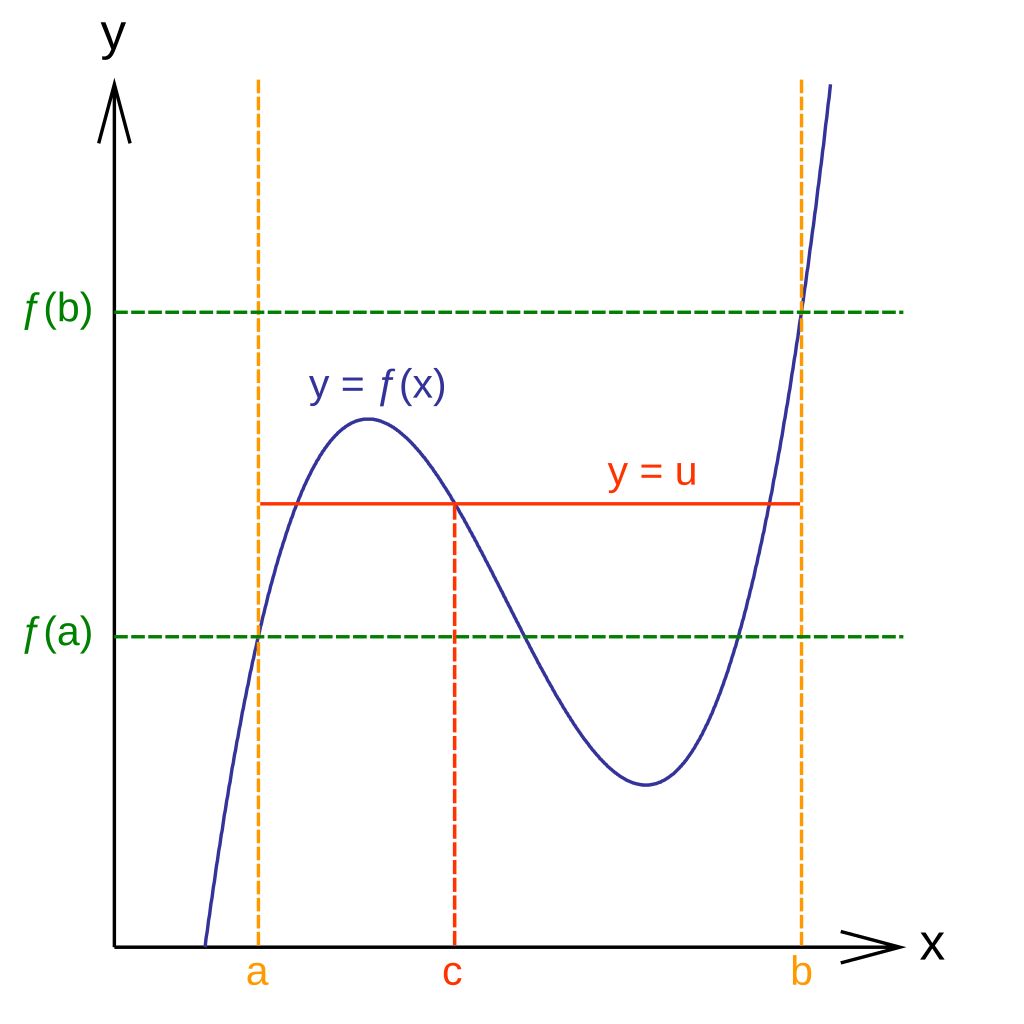
\includegraphics[width=5cm]{intermediate_value_thm}
    \caption{Intermediate value theorem. Source: \href{https://en.wikipedia.org/wiki/Intermediate_value_theorem}{Wikipediat{\tt/}intermediate value theorem}.}
\end{figure}
This captures an intuitive property of continuous functions over the real numbers: given $f$ continuous on $[a,b]$, for $a,b\in\mathbb{R}$, $a < b$, with the known values $f(a) = \alpha,f(b) = \beta$, then the graph of $y = f(x)$ must pass through the horizontal line $y = \dfrac{\alpha + \beta}{2}$ while $x$ moves from $\alpha$ to $\beta$. It represents the idea that the graph of a continuous function on a closed interval can be drawn without lifting a pencil from the paper.

-- Điều này nắm bắt được 1 tính chất trực quan của các hàm liên tục trên các số thực: cho $f$ liên tục trên $[a,b]$, với $a,b\in\mathbb{R}$, $a < b$, với các giá trị đã biết $f(a) = \alpha,f(b) = \beta$, thì đồ thị của $y = f(x)$ phải đi qua đường thẳng nằm ngang $y = \dfrac{\alpha + \beta}{2}$ trong khi $x$ di chuyển từ $\alpha$ đến $\beta$. Nó thể hiện ý tưởng rằng đồ thị của 1 hàm liên tục trên 1 khoảng đóng có thể được vẽ mà không cần nhấc bút chì khỏi giấy.

\begin{theorem}[Intermediate value theorem]
    Consider the closed interval $I = [a,b]\subset\mathbb{R}$ \& a continuous function $f:I\to\mathbb{R}$. Then:
    \item(i) {\rm(Version I)} If $\alpha$ is a number between $f(a)$ \& $f(b)$, i.e., $\min\{f(a),f(b)\} < \alpha < \max\{f(a),f(b)\}$, or $\alpha\in(\min\{f(a),f(b)\},\max\{f(a),f(b)\})$, then there is a $c\in(a,b)$ s.t. $f(c) = \alpha$.
    \item(ii) {\rm(Version II)} The image set $f(I)$ is also a closed interval, \& it contains $[\min\{f(a),f(b)\},\max\{f(a),f(b)\}]$.
\end{theorem}
For a proof, see any standard mathematical analysis textbook, or \href{https://en.wikipedia.org/wiki/Intermediate_value_theorem#Proof}{Wikipedia{\tt/}intermediate value theorem{\tt/}proof}.

\begin{remark}
    The intermediate value theorem can also be proved using the methods of non-standard analysis, which places ``intuitive'' arguments involving infinitesimals on a rigorous footing.
    
    -- Định lý giá trị trung gian cũng có thể được chứng minh bằng các phương pháp phân tích phi chuẩn, trong đó đặt các lập luận ``trực quan'' liên quan đến vô cùng nhỏ vào 1 nền tảng chặt chẽ.
\end{remark}

%------------------------------------------------------------------------------%

\subsection{Relation to completeness -- Quan hệ với tính đầy đủ}
The theorem depends on, \& is equivalent to, the \href{https://en.wikipedia.org/wiki/Completeness_of_the_real_numbers}{completeness of $\mathbb{R}$}. The intermediate value theorem does not apply to the \href{https://en.wikipedia.org/wiki/Rational_number}{rational numbers} $\mathbb{Q}$ because gaps exist between rational numbers; \href{https://en.wikipedia.org/wiki/Irrational_numbers}{irrational numbers} fill those gaps.

-- Định lý phụ thuộc vào \& tương đương với tính đầy đủ của $\mathbb{R}$. Định lý giá trị trung gian không áp dụng cho các số hữu tỉ $\mathbb{Q}$ vì có khoảng trống giữa các số hữu tỉ; các số vô tỉ lấp đầy các khoảng trống đó.

\begin{example}[$f:\mathbb{Q}\to\mathbb{Q}$, $x\mapsto x^2$]
    The function $f(x) = x^2$ for $x\in\mathbb{Q}$ satisfies $f(0) = 0,f(2) = 4$. However, there is no rational number $x\in\mathbb{Q}$ s.t. $f(x) = 2$, because $\sqrt{2}$ is an irrational number.
    
    -- Hàm $f(x) = x^2$ đối với $x\in\mathbb{Q}$ thỏa mãn $f(0) = 0,f(2) = 4$. Tuy nhiên, không có số hữu tỉ $x\in\mathbb{Q}$ s.t. $f(x) = 2$, vì $\sqrt{2}$ là 1 số vô tỉ.
\end{example}
Despite the above, there is a version of the intermediate value theorem for polynomials over a \href{https://en.wikipedia.org/wiki/Real_closed_field}{real closed field}; see the \href{https://en.wikipedia.org/wiki/Weierstrass_Nullstellensatz}{Weierstrass Nullstellensatz}.

-- Bất chấp những điều trên, vẫn có 1 phiên bản của định lý giá trị trung gian cho đa thức trên 1 trường thực đóng.

In mathematics, the {\it Weierstrass Nullstellensatz} is a version of the intermediate value theorem over a real closed field:

\begin{theorem}[Weierstrass Nullstellensatz]
    Given a polynomial $f$ in $1$ variable with coefficients in a real closed field $F$ \& $a < b$ in $F$, if $f(a) < 0 < f(b)$, then there exists a $c\in F$ s.t. $a < c < b$ \& $f(c) = 0$.
\end{theorem}

\begin{proof}
    Since $F$ is real-closed, $F(i)$ is algebraically closed, hence $f(x)$ can be written as $a\prod_i (x - \alpha_i)$ where $a\in F$ is the leading coefficient \& $\alpha_j\in F(i)$ are the roots of $f$. Since each nonreal root $\alpha_j = a_j + ib_j$ can be paired with its conjugate $\overline{\alpha}_j = a_j - ib_j$ (which is also a root of $f$), $f$ can be factored in $F[x]$ as a product of linear polynomials \& polynomials of the form $(x - \alpha_j)(x - \overline{\alpha}_j) = (x - \alpha_j)^2 + b_j^2$, $b_j\ne0$. If $f$ changes sign between $a$ \& $b$, 1 of these factors must change sign. But $(x - a_j)^2 + b_j^2$ is strictly positive for all $x$ in any formally real field, hence 1 of the linear factors $x - \alpha_j$, $\alpha_j\in F$, must change sign between $a$ \& $b$, i.e., the root $\alpha_j$ of $f$ satisfies $a < \alpha_j < b$.
    
    -- Vì $F$ thực đóng, nên $F(i)$ đóng đại số, do đó $f(x)$ có thể được viết thành $a\prod_i (x - \alpha_i)$ với $a\in F$ là hệ số cao nhất \& $\alpha_j\in F(i)$ là các nghiệm của $f$. Vì mỗi nghiệm không thực $\alpha_j = a_j + ib_j$ có thể ghép với nghiệm liên hợp của nó $\overline{\alpha}_j = a_j - ib_j$ (cũng là 1 nghiệm của $f$), nên $f$ có thể được phân tích trong $F[x]$ dưới dạng tích của các đa thức tuyến tính \& các đa thức có dạng $(x - \alpha_j)(x - \overline{\alpha}_j) = (x - \alpha_j)^2 + b_j^2$, $b_j\ne0$. Nếu $f$ đổi dấu giữa $a$ \& $b$, 1 trong các thừa số này phải đổi dấu. Nhưng $(x - a_j)^2 + b_j^2$ là số dương nghiêm ngặt đối với mọi $x$ trong bất kỳ trường thực chính thức nào, do đó 1 trong các thừa số tuyến tính $x - \alpha_j$, $\alpha_j\in F$, phải đổi dấu giữa $a$ \& $b$, tức là, gốc $\alpha_j$ của $f$ thỏa mãn $a < \alpha_j < b$.
\end{proof}

\begin{remark}[Cf. Version I vs. version II of intermediate value theorem]
    Version II states that the set of function values has no gap. For any $2$ function values $c,d\in f(I)$ with $c < d$, all points in the interval $[c,d]$ are also function values, i.e., $[c,d]\subseteq f(I)$. A subset of the real numbers with no internal gap is an interval. Version I is naturally contained in Version II.
    
    -- Phiên bản II nêu rằng tập hợp các giá trị hàm không có khoảng trống. Đối với bất kỳ $2$ giá trị hàm $c,d\in f(I)$ nào với $c < d$, tất cả các điểm trong khoảng $[c,d]$ cũng là các giá trị hàm, tức là $[c,d]\subseteq f(I)$. Một tập hợp con của các số thực không có khoảng trống bên trong là 1 khoảng. Phiên bản I tự nhiên có trong Phiên bản II.
\end{remark}

%------------------------------------------------------------------------------%

\subsection{History of intermediate value theorem}
A form of the theorem was postulated as early as the 5th century BCE, in the work of \href{https://en.wikipedia.org/wiki/Bryson_of_Heraclea}{Bryson of Heraclea} on \href{https://en.wikipedia.org/wiki/Squaring_the_circle}{squaring the circle}. {\sc Bryan} argued that, as circles larger \& smaller than a given square both exist, there must exist a circle of equal area. The theorem was 1st proved by {\sc Bernard Bolzano} in 1817. \href{https://en.wikipedia.org/wiki/Bernard_Bolzano}{\sc Bolzano} used the following formulation of the theorem:

-- 1 dạng của định lý đã được đưa ra từ thế kỷ thứ 5 trước Công nguyên, trong tác phẩm của Bryson xứ Heraclea về việc bình phương hình tròn. {\sc Bryan} lập luận rằng, vì các hình tròn lớn hơn \& nhỏ hơn 1 hình vuông cho trước đều tồn tại, nên phải tồn tại 1 hình tròn có diện tích bằng nhau. Định lý lần đầu tiên được {\sc Bernard Bolzano} chứng minh vào năm 1817. {\sc Bolzano} đã sử dụng công thức sau của định lý:

\begin{theorem}
    Let $f,\varphi$ be continuous functions on the interval between $\alpha,\beta$ s.t. $f(\alpha) < \varphi(\alpha),f(\beta) > \varphi(\beta)$. Then there is an $x$ between $\alpha$ \& $\beta$ s.t. $f(x) = \varphi(x)$.
\end{theorem}
The equivalence between this formulation \& the modern one can be shown by setting $\varphi$ to the appropriate constant function. {\sc Augustin-Louis Cauchy} provided the modern formulation \& a proof in 1821. Both were inspired by the goal of formalizing the analysis of functions \& the work of {\sc Joseph-Louis Lagrange}. The idea that continuous functions possess the intermediate value property has an earlier origin. {\sc Simon Stevin} proved the intermediate value theorem for polynomials (using a cubic as an example) by providing an algorithm for constructing the decimal expansion of the solution. The algorithm iteratively subdivides the interval into 10 parts, producing an additional decimal digit at each step of the iteration. Before the formal definition of continuity was given, the intermediate value property was given as part of the definition of a continuous function. Proponents include {\sc Louis Arbogast}, who assumed the functions to have no jumps, satisfy the intermediate value property \& have increments whose sizes corresponded to the sizes of the increments of the variable. Earlier authors held the result to be intuitively obvious \& requiring no proof. The insight of {\sc Bolzano \& Cauchy} was to define a general notion of continuity (in terms of infinitesimals in {\sc Cauchy}'s case \& using real inequalities in {\sc Bolzano}'s case), \& to provide a proof based on such definitions.

-- Sự tương đương giữa công thức này \& công thức hiện đại có thể được chứng minh bằng cách đặt $\varphi$ thành hàm hằng số thích hợp. {\sc Augustin-Louis Cauchy} đã cung cấp công thức hiện đại \& 1 bằng chứng vào năm 1821. Cả hai đều lấy cảm hứng từ mục tiêu chính thức hóa việc phân tích các hàm \& công trình của {\sc Joseph-Louis Lagrange}. Ý tưởng rằng các hàm liên tục sở hữu tính chất giá trị trung gian có nguồn gốc từ trước đó. {\sc Simon Stevin} đã chứng minh định lý giá trị trung gian cho đa thức (sử dụng 1 khối làm ví dụ) bằng cách cung cấp 1 thuật toán để xây dựng khai triển thập phân của nghiệm. Thuật toán chia nhỏ khoảng thành 10 phần theo cách lặp lại, tạo ra 1 chữ số thập phân bổ sung tại mỗi bước lặp. Trước khi định nghĩa chính thức về tính liên tục được đưa ra, tính chất giá trị trung gian đã được đưa ra như 1 phần của định nghĩa về hàm liên tục. Những người ủng hộ bao gồm {\sc Louis Arbogast}, người cho rằng các hàm không có bước nhảy nào, thỏa mãn thuộc tính giá trị trung gian \& có các gia số có kích thước tương ứng với kích thước của các gia số của biến. Các tác giả trước đó cho rằng kết quả là hiển nhiên theo trực giác \& không cần chứng minh. Nhận thức của {\sc Bolzano \& Cauchy} là định nghĩa 1 khái niệm chung về tính liên tục (theo nghĩa là vô cùng nhỏ trong trường hợp của {\sc Cauchy} \& sử dụng bất đẳng thức thực trong trường hợp của {\sc Bolzano}), \& cung cấp 1 bằng chứng dựa trên các định nghĩa như vậy.

%------------------------------------------------------------------------------%

\subsection{Converse of intermediate value theorem is false -- Chiều đảo của định lý giá trị trung gian là sai}
A \href{https://en.wikipedia.org/wiki/Darboux_function}{Darboux function} is a real-valued function $f$ that has the ``intermediate value property'', i.e., that satisfies the conclusion of the intermediate value theorem: for any 2 values $a,b$ in the domain of $f$, \& any $y$ between $f(a)$ \& $f(b)$, there is some $c$ between $a$ \& $b$ with $f(c) = y$. The intermediate value theorem says that every continuous function is a Darboux funtion. However, not every Darboux function is continuous, i.e., the converse of the intermediate value theorem is false.

-- Hàm Darboux là hàm giá trị thực $f$ có ``tính chất giá trị trung gian'', tức là thỏa mãn kết luận của định lý giá trị trung gian: với bất kỳ 2 giá trị $a,b$ trong miền của $f$, \& bất kỳ $y$ nào nằm giữa $f(a)$ \& $f(b)$, thì có 1 số $c$ nằm giữa $a$ \& $b$ với $f(c) = y$. Định lý giá trị trung gian nói rằng mọi hàm liên tục đều là hàm Darboux. Tuy nhiên, không phải mọi hàm Darboux đều liên tục, tức là, điều ngược lại của định lý giá trị trung gian là sai.

\begin{example}
    The function $f:[0,\infty)\to[-1,1]$ defined by
    \begin{equation*}
        f(x) = \left\{\begin{split}
             &\sin\frac{1}{x}&&\mbox{if } x > 0,\\
             &0&&\mbox{if } x = 0,
        \end{split}\right.
    \end{equation*}
    is not continuous at $x = 0$ because the limit of $f(x)$ as $x$ tends to $0$ does not exist; yet the function has the intermediate value property.
\end{example}
Another, more complicated example is given by the \href{https://en.wikipedia.org/wiki/Conway_base_13_function}{conway base 13 function}.

In fact, \href{https://en.wikipedia.org/wiki/Darboux%27s_theorem_(analysis)}{Darboux's theorem} states that all functions that result from the differentiation of some other function on some interval have the intermediate value property (even though they need not be continuous).

-- Trên thực tế, định lý Darboux phát biểu rằng tất cả các hàm là kết quả của phép vi phân của 1 số hàm khác trên 1 khoảng nào đó đều có tính chất giá trị trung gian (mặc dù chúng không nhất thiết phải liên tục).

Historically, this intermediate value property has been suggested as a definition for continuity of real-valued functions; this definition was not adopted.

-- Về mặt lịch sử, tính chất giá trị trung gian này đã được đề xuất như 1 định nghĩa cho tính liên tục của các hàm có giá trị thực; định nghĩa này đã không được chấp nhận.

%------------------------------------------------------------------------------%

\subsection{Generalizations of intermediate value theorem -- Các tổng quát hóa của định lý giá trị trung gian}

%------------------------------------------------------------------------------%

\subsubsection{Multidimensional spaces -- Các không gian nhiều chiều}
The \href{https://en.wikipedia.org/wiki/Poincar%C3%A9-Miranda_theorem}{Poincar\'e--Miranda theorem} is a generalization of the Intermediate value theorem from a (1D) interval to a (2D) rectangle, or more generally, to an $n$-dimensional cube.

-- Định lý Poincar\'e--Miranda là 1 sự tổng quát hóa của định lý giá trị trung gian từ 1 khoảng (1D) đến 1 hình chữ nhật (2D) hoặc tổng quát hơn là đến 1 khối lập phương $n$ chiều.

{\sc Vrahatis} presents a similar generalization to triangles, or more generally, $n$-dimensional \href{https://en.wikipedia.org/wiki/Simplex}{simplices}. Let $D^n$ be an $n$-dimensional simplex with $n + 1$ vertices denoted by $v_0,v_1,\ldots,v_n$. Let $F = (f_1,\ldots,f_n)$ be a continuous function from $D^n\to\mathbb{R}^n$, that never equals 0 on the boundary $\partial D^n$ of $D^n$. Suppose $F$ satisfies the following conditions:
\begin{itemize}
    \item $\forall i\in[n]$, the sign of $f_i(v_i)$ is opposite to the sign of $f_i(x)$ for all points $x$ on the face opposite to $v_i$;
    \item The sign-vector of $f_1,\ldots,f_n$ on $v_0$ is not equal to the sign-vector of $f_1,\ldots,f_n$ on all points on the face opposite to $v_0$.
\end{itemize}
Then there is a point $z$ in the interior of $D^n$ on which $F(z) = (0,\ldots,0)$.

-- {\sc Vrahatis} đưa ra 1 khái quát tương tự cho tam giác, hay nói chung hơn là các đơn hình $n$ chiều. Cho $D^n$ là 1 đơn hình $n$ chiều với $n + 1$ đỉnh được ký hiệu là $v_0,v_1,\ldots,v_n$. Cho $F = (f_1,\ldots,f_n)$ là 1 hàm liên tục từ $D^n\to\mathbb{R}^n$, không bao giờ bằng 0 trên biên $\partial D^n$ của $D^n$. Giả sử $F$ thỏa mãn các điều kiện sau:
\begin{itemize}
    \item $\forall i\in[n]$, dấu của $f_i(v_i)$ ngược với dấu của $f_i(x)$ đối với mọi điểm $x$ trên mặt đối diện với $v_i$;
    \item Vectơ dấu của $f_1,\ldots,f_n$ trên $v_0$ không bằng với vectơ dấu của $f_1,\ldots,f_n$ trên mọi điểm trên mặt đối diện với $v_0$.
\end{itemize}
Khi đó có 1 điểm $z$ ở bên trong $D^n$ mà tại đó $F(z) = (0,\ldots,0)$.

It is possible to normalize the $f_i$ s.t. $f_i(v_i) > 0$, $\forall i\in[n]$; then the conditions become simpler:
\begin{itemize}
    \item $\forall i\in[n]$, $f_i(v_i) > 0$, \& $f_i(x) < 0$ for all points $x$ on the face opposite to $v_i$. In particular, $f_i(v_0) < 0$.
    \item For all points $x$ on the face opposite to $v_0$, $f_i(x) > 0$ for at least 1 $i\in[n]$.
\end{itemize}
The theorem can be proved based on the \href{https://en.wikipedia.org/wiki/Knaster%E2%80%93Kuratowski%E2%80%93Mazurkiewicz_lemma}{Knaster--Kuratowski--Mazurkiewicz lemma}. It can be used for approximations of fixed points \& zeros.

-- Có thể chuẩn hóa $f_i$ s.t. $f_i(v_i) > 0$, $\forall i\in[n]$; khi đó các điều kiện trở nên đơn giản hơn:
\begin{itemize}
    \item $\forall i\in[n]$, $f_i(v_i) > 0$, \& $f_i(x) < 0$ cho mọi điểm $x$ trên mặt đối diện với $v_i$. Cụ thể, $f_i(v_0) < 0$.
    \item Đối với mọi điểm $x$ trên mặt đối diện với $v_0$, $f_i(x) > 0$ cho ít nhất 1 $i\in[n]$.
\end{itemize}
Định lý có thể được chứng minh dựa trên định lý Knaster--Kuratowski--Mazurkiewicz. Định lý này có thể được sử dụng để xấp xỉ các điểm cố định \& nghiệm.

%------------------------------------------------------------------------------%

\subsubsection{General metric \& topological spaces -- Các không gian metric \& tôpô tổng quát}
The intermediate value theorem is closely linked to the topological notion of connectedness \& follows from the basic properties of connected sets in metric spaces \& connected subsets of $\mathbb{R}$ in particular:
\begin{itemize}
    \item If $X,Y$ are metric spaces, $f:X\to Y$ is a continuous map, \& $E\subset X$ is a connected subset, then $f(E)$ is connected. (*)
    \item A subset $E\subset\mathbb{R}$ is connected iff it satisfies the following property: $x,y\in E,x < r < y\Rightarrow r\in E$. (**)
\end{itemize}
In fact, connectedness is a topological property \& (*) generalizes to topological spaces:

\begin{theorem}
    If $X,Y$ are topological spaces, $f:X\to  Y$ is a continuous map, \& $X$ is a connected space, then $f(X)$ is connected.
\end{theorem}
The preservation of connectedness under continuous maps can be thought of as a generalization of the intermediate value theorem, a property of continuous, real-valued functions of a real variable, to continuous functions in general spaces.

-- Định lý giá trị trung gian có liên quan chặt chẽ với khái niệm tôpô về tính liên thông \& tuân theo các tính chất cơ bản của các tập liên thông trong không gian metric \& các tập con liên thông của $\mathbb{R}$ nói riêng:
\begin{itemize}
    \item Nếu $X,Y$ là các không gian metric, $f:X\to Y$ là 1 ánh xạ liên tục, \& $E\subset X$ là 1 tập con liên thông, thì $f(E)$ là liên thông. (*)
    \item Một tập con $E\subset\mathbb{R}$ là liên thông khi và chỉ khi nó thỏa mãn tính chất sau: $x,y\in E,x < r < y\Rightarrow r\in E$. (**)
\end{itemize}
Trên thực tế, tính liên thông là 1 tính chất tôpô \& (*) được khái quát hóa thành các không gian tôpô:

\begin{dinhly}
    Nếu $X,Y$ là các không gian tôpô, $f:X\to Y$ là 1 ánh xạ liên tục, \& $X$ là 1 không gian liên thông, thì $f(X)$ liên thông.
\end{dinhly}
Việc bảo toàn tính liên thông trong các ánh xạ liên tục có thể được coi là khái quát hóa của định lý giá trị trung gian, 1 tính chất của các hàm liên tục, có giá trị thực của 1 biến thực, thành các hàm liên tục trong các không gian tổng quát.

The intermediate value theorem generalizes in a natural way: Suppose that $X$ is a connected topological space \& $(Y,<)$ is a \href{https://en.wikipedia.org/wiki/Total_order}{totally ordered} set equipped with the \href{https://en.wikipedia.org/wiki/Order_topology}{order topology}, \& let $f:X\to Y$ be a continuous map. If $a,b$ are 2 points in $X$ \& $u$ is a point in $Y$ lying between $f(a)$ \& $f(b)$ w.r.t. $<$, then there exists $c\in X$ s.t. $f(c) = u$. The original theorem is recovered by noting that $\mathbb{R}$ is connected \& that its natural topology is the order topology. The \href{https://en.wikipedia.org/wiki/Brouwer_fixed-point_theorem}{Brouwer fixed-point theorem} is a related theorem that, in 1D, gives a special case of the intermediate value theorem.

-- Định lý giá trị trung gian được tổng quát hóa theo cách tự nhiên: Giả sử $X$ là 1 không gian tôpô liên thông \& $(Y,<)$ là 1 tập hợp được sắp thứ tự toàn phần được trang bị tôpô thứ tự, \& cho $f:X\to Y$ là 1 ánh xạ liên tục. Nếu $a,b$ là 2 điểm trong $X$ \& $u$ là 1 điểm trong $Y$ nằm giữa $f(a)$ \& $f(b)$ w.r.t. $<$, thì tồn tại $c\in X$ s.t. $f(c) = u$. Định lý ban đầu được phục hồi bằng cách lưu ý rằng $\mathbb{R}$ là liên thông \& rằng tôpô tự nhiên của nó là tôpô thứ tự. Định lý điểm bất động Brouwer là 1 định lý liên quan, trong 1D, đưa ra 1 trường hợp đặc biệt của định lý giá trị trung gian.

%------------------------------------------------------------------------------%

\subsection{Intermediate value theorem in constructive mathematics -- Định lý giá trị trung gian trong toán học xây dựng}
In constructive mathematics, the ntermediate value theorem is not true. Instead, the weakened conclusion one must take states that the value may only be found in some range which may be arbitrarily small.

-- Trong toán học xây dựng, định lý giá trị trung gian không đúng. Thay vào đó, kết luận yếu hơn mà người ta phải đưa ra là giá trị chỉ có thể được tìm thấy trong 1 phạm vi nào đó có thể nhỏ tùy ý.

\begin{theorem}
    Let $a,b\in\mathbb{R}$, $f:[a,b]\to\mathbb{R}$ be a pointwise continuous function from the closed interval $[a,b]$ to the real line, \& suppose that $f(a) < 0 < f(b)$. Then for every $\varepsilon\in(0,\infty)$, there exists a point $x$ in the unit interval s.t. $|f(x)| < \varepsilon$.
\end{theorem}

\begin{dinhly}
    Cho $a,b\in\mathbb{R}$, $f:[a,b]\to\mathbb{R}$ là 1 hàm liên tục từng điểm từ khoảng đóng $[a,b]$ đến đường thẳng thực, \& giả sử rằng $f(a) < 0 < f(b)$. Khi đó, với mọi $\varepsilon\in(0,\infty)$, tồn tại 1 điểm $x$ trong khoảng đơn vị s.t. $|f(x)| < \varepsilon$.
\end{dinhly}

%------------------------------------------------------------------------------%

\subsection{Practical applications of intermediate value theorem -- Ứng dụng thực thế của định lý giá trị trung gian}
A similar result is the \href{https://en.wikipedia.org/wiki/Borsuk%E2%80%93Ulam_theorem}{Borsuk--Ulam theorem}, which says that a continuous map from the $n$-sphere to Euclidean $n$-space will always map some pair of antipodal points to the same place.

-- 1 kết quả tương tự là định lý Borsuk--Ulam, nói rằng 1 phép ánh xạ liên tục từ mặt cầu $n$ sang không gian Euclid $n$ sẽ luôn ánh xạ 1 số cặp điểm đối cực tới cùng 1 vị trí.

In general, for any continuous function whose domain is some closed convex $n$-dimensional shape \& any point inside the shape (not necessarily its center), there exist 2 antipodal points w.r.t. the given point whose functional value is the same.

-- Nhìn chung, đối với mọi hàm liên tục có miền xác định là 1 hình lồi khép kín n chiều \& bất kỳ điểm nào bên trong hình đó (không nhất thiết phải là tâm của hình đó), thì tồn tại 2 điểm đối cực so với điểm đã cho có giá trị hàm giống nhau.
\begin{proof}[Proof for 1D case]
    Take $f$ to be any continuous function on a circle. Draw a line through the center of the circle, intersecting it at $2$ opposite points $A,B$. Define $d\coloneqq f(A) - f(B)$. If the line is rotated $180^\circ$, the value $-d$ will be obtained instead. Due to the intermediate value theorem there must be some intermediate rotation angle for which $d = 0$, \& as a consequence $f(A) = f(B)$ at this angle.
    
    -- Cho $f$ là 1 hàm liên tục bất kỳ trên 1 đường tròn. Vẽ 1 đường thẳng đi qua tâm của đường tròn, cắt nó tại $2$ điểm đối diện $A,B$. Định nghĩa $d\coloneqq f(A) - f(B)$. Nếu đường thẳng được quay $180^\circ$, giá trị $-d$ sẽ thu được thay thế. Do định lý giá trị trung gian, phải có 1 số góc quay trung gian mà $d = 0$, \& do đó $f(A) = f(B)$ ở góc này.
\end{proof}
The theorem also underpins the explanation of why rotating a wobbly table will bring it to stability (subject to certain easily met constraints).

-- Định lý này cũng củng cố lời giải thích tại sao việc xoay 1 chiếc bàn rung lắc sẽ đưa nó đến trạng thái ổn định (tùy thuộc vào 1 số ràng buộc dễ đáp ứng).

\begin{baitoan}[Discrete version of intermediate value theorem]
    Investigate on the discrete version of the intermediate value theorem.
    
    -- Tìm hiểu dạng rời rạc của định lý giá trị trung gian.
\end{baitoan}
E.g., see DAK's CP solution for IMO2007 Problem 3 \href{github.com/NQBH/advanced_STEM_beyond/blob/main/OLP_ICPC/resource/DAK_IMO2007_P3.pdf}, trong đó lý luận ``$D_i = k_{1,i} - k_{2,i}$ sẽ giảm dần từ 1 số không âm xuống 1 số âm. Vì $D_i$ là 1 chuỗi số nguyên \& mỗi bước chỉ thay đổi 1 lượng nhỏ, nó chắn chắn sẽ đi qua giá trị 0. Khi $D_i = 0$, ta có $k_{1,i} = k_{2,i}$. Đây chính là trạng thái cân bằng mà ta cần tìm.'' chính là dạng rời rạc của định lý giá trị trung gian phiên bản 2 giá trị trái dấu với nhau $f(a)f(b) < 0$.

%------------------------------------------------------------------------------%

\section{Interior Extremum Theorem{\tt/}Fermat Theorem -- Định Lý Cực Trị Bên Trong{\tt/}Định Lý Fermat}
\textbf{\textsf{Resources -- Tài nguyên.}}
\begin{enumerate}
    \item \href{https://en.wikipedia.org/wiki/Interior_extremum_theorem}{Wikipedia{\tt/}interior extremum theorem}.
\end{enumerate}
In mathematics, the {\it interior extremum theorem}, also known as {\it Fermat's theorem}, is a theorem which states that at the \href{https://en.wikipedia.org/wiki/Local_extrema}{local extrema} of a \href{https://en.wikipedia.org/wiki/Differentiable_function}{differentiable function}, its derivative is always 0. It belongs to the mathematical field of \href{https://en.wikipedia.org/wiki/Real_analysis}{real analysis} \& is named after French mathematician \href{https://en.wikipedia.org/wiki/Pierre_de_Fermat}{\sc Pierre de Fermat}.

-- Trong toán học, {\it định lý cực trị trong}, còn được gọi là {\it định lý Fermat}, là 1 định lý phát biểu rằng tại cực trị cục bộ của 1 hàm khả vi, đạo hàm của nó luôn bằng 0. Nó thuộc lĩnh vực toán học giải tích thực \& được đặt theo tên của nhà toán học người Pháp {\sc Pierre de Fermat}.

By using the interior extremum theorem, the potential extrema of a function $f$, with derivative $f'$, can be found by solving an equation involving $f'$. The interior extremum theorem gives only a necessary condition for extreme function values, as some stationary points are inflection points (not a maximum or minimum). The function's 2nd derivative, if it exists, can sometimes be used to determine whether a stationary point is a maximum or minimum.

-- Bằng cách sử dụng định lý cực trị trong, cực trị tiềm tàng của 1 hàm $f$, với đạo hàm $f'$, có thể được tìm thấy bằng cách giải 1 phương trình liên quan đến $f'$. Định lý cực trị trong chỉ đưa ra 1 điều kiện cần thiết cho các giá trị cực trị của hàm, vì 1 số điểm dừng là điểm uốn (không phải là điểm cực đại hay cực tiểu). Đạo hàm bậc 2 của hàm, nếu có, đôi khi có thể được sử dụng để xác định xem 1 điểm dừng là điểm cực đại hay cực tiểu.
\begin{figure}[H]
    \centering
    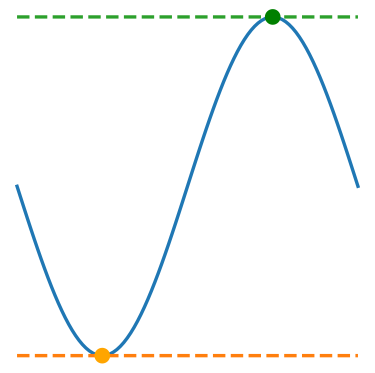
\includegraphics[width=5cm]{interior_extremum_graph}
    \caption{A differentiable function graph with lines tangent to the minimum \& maximum. The interior extremum theorem guarantees that these lines will always be horizontal. -- Đồ thị hàm số khả vi với các đường tiếp tuyến với giá trị nhỏ nhất \& lớn nhất. Định lý cực trị trong đảm bảo rằng các đường này sẽ luôn nằm ngang.}
\end{figure}

\paragraph*{History.} {\sc Pierre de Fermat} proposed in a collection of treatises titled {\it Maxima et minima} a method to find maximum or minimum, similar to the modern interior extremum theorem, albeit with the use of infiniesimals rather than derivatives. After {\sc Marin Mersenne} passed the treatises onto {\sc Ren\'e Descartes}, {\sc Descartes} was doubtful, remarking ``if [$\ldots$] he speaks of wanting to send you still more papers, I beg of you to ask him to think them out more carefully than those preceding''. {\sc Descartes} later agreed that the method was valid.

-- {\sc Pierre de Fermat} đã đề xuất trong 1 tập hợp các chuyên luận có tựa đề {\it Maxima et minima} 1 phương pháp để tìm giá trị cực đại hoặc cực tiểu, tương tự như định lý cực trị nội tại hiện đại, mặc dù sử dụng các số vô cùng nhỏ thay vì đạo hàm. Sau khi {\sc Marin Mersenne} chuyển các chuyên luận cho {\sc Ren\'e Descartes}, {\sc Descartes} tỏ ra nghi ngờ, nhận xét rằng ``nếu [$\ldots$] ông ấy nói muốn gửi cho bạn nhiều bài báo hơn nữa, tôi cầu xin bạn hãy yêu cầu ông ấy suy nghĩ kỹ hơn về chúng so với những bài trước đó''. {\sc Descartes} sau đó đã đồng ý rằng phương pháp này là hợp lệ.

1 way to state the interior extremum theorem is that, if a function has a local extremum at some point \& is differentiable there, then the function's derivative at that point must be 0. In precise mathematical language:

-- 1 cách để phát biểu định lý cực trị trong là nếu 1 hàm có cực trị cục bộ tại 1 điểm \& khả vi tại đó, thì đạo hàm của hàm tại điểm đó phải bằng 0. Theo ngôn ngữ toán học chính xác:

\begin{theorem}[Fermat's theorem]
    Let $f:(a,b)\to\mathbb{R}$ be a function from an open interval $(a,b)$ to $\mathbb{R}$, \& suppose that $x_0\in(a,b)$ is a point where $f$ has a local extremum. If $f$ is differentiable at $x_0$, then $f'(x_0) = 0$.
\end{theorem}

\begin{proof}
    Suppose that $x_0$ is a local maximum. (A similar argument applies if $x_0$ is a local minimum.) Then there is some neighborhood around $x_0$ s.t. $f(x_0)\ge f(x)$ for all $x$ within that neighborhood. If $x > x_0$, then the \href{https://en.wikipedia.org/wiki/Difference_quotient}{difference quotient} $\frac{f(x) - f(x_0)}{x - x_0}$ is nonpositive for $x$ in this neighborhood. This implies
    \begin{equation*}
        \lim_{x\to x_0^+} \frac{f(x) - f(x_0)}{x - x_0}\le0.
    \end{equation*}
    Similarly, if $x < x_0$, then the difference quotient is nonnegative, \& so
    \begin{equation*}
        \lim_{x\to x_0^-} \frac{f(x) - f(x_0)}{x - x_0}\ge0.
    \end{equation*}
    Since $f$ is differentiable, the above limits must both be equal to $f'(x_0)$. This is only possible if both limits are equal to 0, so $f'(x_0) = 0$.
\end{proof}

\begin{dinhly}[định lý của Fermat]
    Cho $f:(a,b)\to\mathbb{R}$ là 1 hàm từ 1 khoảng mở $(a,b)$ đến $\mathbb{R}$, \& giả sử rằng $x_0\in(a,b)$ là 1 điểm mà $f$ có cực trị cục bộ. Nếu $f$ khả vi tại $x_0$, thì $f'(x_0) = 0$.
\end{dinhly}

\begin{proof}
    Giả sử $x_0$ là cực đại cục bộ. (1 lập luận tương tự được áp dụng nếu $x_0$ là cực tiểu cục bộ.) Khi đó, có 1 số lân cận xung quanh $x_0$ s.t. $f(x_0)\ge f(x)$ cho mọi $x$ trong lân cận đó. Nếu $x > x_0$, thì thương hiệu $\frac{f(x) - f(x_0)}{x - x_0}$ không dương đối với $x$ trong lân cận này. Điều này ngụ ý
    \begin{equation*}
        \lim_{x\to x_0^+} \frac{f(x) - f(x_0)}{x - x_0}\le0.
    \end{equation*}
    Tương tự, nếu $x < x_0$, thì thương hiệu không âm, \& do đó
    \begin{equation*}
        \lim_{x\to x_0^-} \frac{f(x) - f(x_0)}{x - x_0}\ge0.
    \end{equation*}
    Vì $f$ khả vi, nên các giới hạn trên đều phải bằng $f'(x_0)$. Điều này chỉ có thể xảy ra nếu cả hai giới hạn đều bằng 0, do đó $f'(x_0) = 0$.
\end{proof}
Another way to understand the theorem is via the contrapositive statement: if the derivative of a function at any point is not zero, then there is not a local extremum at that point. Formally:

-- 1 cách khác để hiểu định lý này là thông qua câu lệnh phản biện: nếu đạo hàm của 1 hàm tại bất kỳ điểm nào không bằng 0, thì không có cực trị cục bộ tại điểm đó. Về mặt hình thức:

\begin{theorem}
    If $f$ is differentiable at $x_0\in(a,b)$, \& $f'(x_0)\ne0$, then $x_0$ is not a local extremum of $f$.
\end{theorem}

\begin{dinhly}
    Nếu $f$ khả vi tại $x_0\in(a,b)$, \& $f'(x_0)\ne0$, thì $x_0$ không phải là cực trị địa phương của $f$.
\end{dinhly}

\begin{corollary}
    The global extrema of a function $f$ on a domain $A$ occur only at boundaries, non-differentiable points, \& stationary points. If $x_0$ is a global extremum of $f$, then 1 of the following is true:
    \item(i) {\rm boundary:} $x_0$ is in the boundary of $A$: $x_0\in\partial A$.
    \item(ii) {\rm non-differentiable:} $f$ is not differentiable at $x_0$.
    \item(iii) {\rm stationary point:} $x_0$ is a stationary point of $f$.
\end{corollary}

\begin{hequa}
    Cực trị toàn cục của hàm $f$ trên miền $A$ chỉ xảy ra tại các ranh giới, các điểm không khả vi, \& các điểm dừng. Nếu $x_0$ là cực trị toàn cục của $f$, thì 1 trong các điều sau đây là đúng:
    \item(i) {\rm biên:} $x_0$ nằm trong ranh giới của $A$: $x_0\in\partial A$.
    \item(ii) {\rm không khả vi:} $f$ không khả vi tại $x_0$.
    \item(iii) {\rm điểm dừng:} $x_0$ là 1 điểm dừng của $f$.
\end{hequa}

\paragraph*{Extension of interior extreme theorem -- Mở rộng của định lý điểm cực trị bên trong.} A similar statement holds for the partial derivatives of multivariate functions. -- 1 tuyên bố tương tự cũng đúng đối với đạo hàm riêng của hàm đa biến.

\begin{theorem}
    Suppose that some real-valued function of the real numbers $f = f(t_1,t_2,\ldots,t_k)$ has an extreme at a point $C$, defined by $C = (a_1,a_2,\ldots,a_k)$. If $f$ is differentiable at $C$, then $\partial_{t_i}f(a_i) = \frac{\partial}{\partial t_i}f(a_i) = 0$, where $i\in[k]$.
\end{theorem}

\begin{dinhly}
    Giả sử rằng 1 hàm số giá trị thực nào đó của các số thực $f = f(t_1,t_2,\ldots,t_k)$ có cực trị tại 1 điểm $C$, được xác định bởi $C = (a_1,a_2,\ldots,a_k)$. Nếu $f$ khả vi tại $C$, thì $\partial_{t_i}f(a_i) = \frac{\partial}{\partial t_i}f(a_i) = 0$, trong đó $i\in[k]$.
\end{dinhly}
The statement can also be extended to differentiable manifolds. If $f:M\to\mathbb{R}$ is a differentiable function on a manifold $M$, then its local extrema must be critical points of $f$, in particular points where the exterior derivative $df$ is zero.

-- Phát biểu này cũng có thể được mở rộng thành các đa tạp khả vi. Nếu $f:M\to\mathbb{R}$ là 1 hàm khả vi trên 1 đa tạp $M$, thì cực trị cục bộ của nó phải là các điểm tới hạn của $f$, đặc biệt là các điểm mà đạo hàm ngoài $df$ bằng không.

\paragraph*{Applications of interior extremum theorem -- Các ứng dụng của định lý điểm cực trị bên trong.} The interior extremum theorem is central for determining \href{https://en.wikipedia.org/wiki/Maxima_and_minima}{maxima \& minima} of \href{https://en.wikipedia.org/wiki/Piecewise_function}{piecewise differentiable functions} of 1 variable: an extreme is either a \href{https://en.wikipedia.org/wiki/Stationary_point}{stationary point} (i.e., a zero of the derivative), a non-differentiable point (i.e., a point where the function is not differentiable), or a \href{https://en.wikipedia.org/wiki/Boundary_point}{boundary point} of the domain of the function. Since the number of these points is typically finite, the computation of the values of the function at these points provide the maximum \& the minimum, simply by comparing the obtained values.

-- Định lý cực trị bên trong đóng vai trò trung tâm trong việc xác định cực đại \& cực tiểu của các hàm khả vi từng phần của 1 biến: cực trị là điểm dừng (tức là điểm không của đạo hàm), điểm không khả vi (tức là điểm mà hàm không khả vi), hoặc điểm biên của miền xác định của hàm. Vì số lượng các điểm này thường hữu hạn, nên việc tính toán các giá trị của hàm tại các điểm này cung cấp giá trị cực đại \& cực tiểu, chỉ bằng cách so sánh các giá trị thu được.

%------------------------------------------------------------------------------%

\section{Rolle's Theorem -- Định Lý Rolle}
\textbf{\textsf{Resources -- Tài nguyên.}}
\begin{enumerate}
    \item \href{https://en.wikipedia.org/wiki/Rolle%27s_theorem}{Wikipedia{\tt/}Rolle theorem}.
\end{enumerate}
In calculus, {\it Rolle's theorem} or {\it Rolle's lemma} essentially states that any real-valued differentiable function that attains equal values at 2 distinct points must have at least 1 point, somewhere between them, at which the slope of the tangent line is zero. Such a point is known as a \href{https://en.wikipedia.org/wiki/Stationary_point}{tationary point}. It is a point at which the 1st derivative of the function is zero. The theorem is named after \href{https://en.wikipedia.org/wiki/Michel_Rolle}{\sc Michel Rolle}.

-- Trong phép tính vi phân, {\it Định lý Rolle} hoặc {\it Bổ đề Rolle} về cơ bản nêu rằng bất kỳ hàm số khả vi giá trị thực nào đạt được các giá trị bằng nhau tại 2 điểm phân biệt phải có ít nhất 1 điểm, ở đâu đó giữa chúng, mà tại đó độ dốc của đường tiếp tuyến bằng không. Một điểm như vậy được gọi là điểm dừng. Đó là điểm mà đạo hàm bậc 1 của hàm bằng không. Định lý được đặt theo tên của {\sc Michel Rolle}.

\paragraph*{Standard version of Rolle's theorem -- Phiên bản chuẩn của định lý Rolle.}

\begin{theorem}
    If a real-valued function $f$ is continuous on a proper closed interval $[a,b]$, differentiable on the open interval $(a,b)$, \& $f(a) = f(b)$, then there exists at least 1 $c$ in the open interval $(a,b$ s.t. $f'(c) = 0$.
\end{theorem}

\begin{dinhly}[Rolle]
    Nếu 1 hàm số thực $f$ liên tục trên 1 khoảng đóng thực sự $[a,b]$, khả vi trên khoảng mở $(a,b)$, \& $f(a) = f(b)$, thì tồn tại ít nhất 1 $c$ trong khoảng mở $(a,b$ sao cho $f'(c) = 0$.
\end{dinhly}

\begin{dinhly}[Rolle]
    Giả sử $f(x)$ xác định \& liên tục trên $[a,b]$ hữu hạn, khả vi trên $(a,b)$ \& $f(a) = f(b)$. Khi đó tồn tại $c\in(a,b)$ sao cho $f'(c) = 0$.
\end{dinhly}
This version of Rolle's theorem is used to prove the \href{https://en.wikipedia.org/wiki/Mean_value_theorem}{mean value theorem}, of which Rolle's theorem is indeed a special case. It is also the basis for the proof of \href{https://en.wikipedia.org/wiki/Taylor%27s_theorem}{Taylor's theorem}.

-- Phiên bản này của định lý Rolle được sử dụng để chứng minh định lý giá trị trung bình, trong đó định lý Rolle thực sự là 1 trường hợp đặc biệt. Nó cũng là cơ sở cho chứng minh định lý Taylor.

\paragraph*{History.} Although the theorem is named after {\sc Michel Rolle, Rolle}'s 1691 proof covered only the case of polynomial functions. His proof did not use the methods of \href{https://en.wikipedia.org/wiki/Differential_calculus}{differential calculus}, which at that point in his life he considered to be fallacious. The theorem was 1st proved by {\sc Cauchy} in 1823 as a corollary of a proof of the mean value theorem. The name ``Rolle's theorem'' was 1st used by \href{https://en.wikipedia.org/wiki/Moritz_Wilhelm_Drobisch}{\sc Moritz Wilhelm Drobisch} of Germany in 1834 \& by \href{https://en.wikipedia.org/wiki/Giusto_Bellavitis}{\sc Giusto Bellavitis} of Italy in 1846.

-- Mặc dù định lý được đặt theo tên của {\sc Michel Rolle}, bằng chứng năm 1691 của Rolle chỉ bao gồm trường hợp của các hàm đa thức. Bằng chứng của ông không sử dụng các phương pháp của phép tính vi phân, mà tại thời điểm đó trong cuộc đời ông, ông coi là sai lầm. Định lý lần đầu tiên được {\sc Cauchy} chứng minh vào năm 1823 như là hệ quả của 1 bằng chứng về định lý giá trị trung bình. Tên gọi ``Định lý Rolle'' lần đầu tiên được {\sc Moritz Wilhelm Drobisch} của Đức sử dụng vào năm 1834 \& bởi {\sc Giusto Bellavitis} của Ý vào năm 1846.

\begin{example}[Half circle -- nửa đường tròn]
    For a radius $r\in(0,\infty)$, consider the function $f(x) = \sqrt{r^2 - x^2}$, $x\in[-r,r]$. Its graph is the upper semicircle centered at the origin. This function is continuous on the closed interval $[-r,r]$ \& differentiable in the open interval $(-r,r)$, but not differentiable at the endpoints $\pm r$. Since $f(-r) = f(r)$, Rolle's theorem applies, \& indeed, there is a point where the derivative of $f$ is zero. The theorem applies even when the function cannot be differentiated at the endpoints because it only requires the function to be differentiable in the open interval.
    \begin{figure}[H]
        \centering
        \includegraphics[width=4cm]{semicircle}
        \caption{A semicircle of radius $r\in(0,\infty)$.}
    \end{figure}
    -- Với bán kính $r\in(0,\infty)$, xét hàm $f(x) = \sqrt{r^2 - x^2}$, $x\in[-r,r]$. Đồ thị của hàm này là nửa đường tròn trên có tâm tại gốc tọa độ. Hàm này liên tục trên đoạn đóng $[-r,r]$ \& khả vi trên đoạn mở $(-r,r)$, nhưng không khả vi tại các điểm cuối $\pm r$. Vì $f(-r) = f(r)$, nên định lý Rolle được áp dụng, \& thực vậy, có 1 điểm mà đạo hàm của $f$ bằng không. Định lý này được áp dụng ngay cả khi hàm không thể được vi phân tại các điểm cuối vì nó chỉ yêu cầu hàm khả vi trên đoạn mở.
    
    Indeed,
    \begin{equation*}
        f'(x) = -\frac{x}{\sqrt{r^2 - x^2}},\ \forall x\in(-r,r)\mbox{ thus } f'(x) = 0\Leftarrow x = 0.
    \end{equation*}
\end{example}

\begin{example}[Absolute value function -- Hàm giá trị tuyệt đối]
    If differentiability fails at an interior point of the interval, the conclusion of Rolle's theorem may not hold. Consider the \href{https://en.wikipedia.org/wiki/Absolute_value}{absolute value} function $f(x) = |x|$, $x\in[-1,1]$. Then $f(-1) = f(1)$, but there is no $c\in(-1,1$ for which $f'(c) = 0$. This is because that function, although continuous, is not differentiable at $x = 0$, but without attaining the value 0. The theorem cannot be applied to this function because it does not satisfy the condition that the function must be differentiable for every $x$ in the open interval. However, when the differentiability requirement is dropped from Rolle's theorem, $f$ will still have a \href{https://en.wikipedia.org/wiki/Critical_number}{critical number} in the open interval $(a,b)$, but it may not yield a horizontal tangent (as in the case of the absolute value represented in the graph).
    \begin{figure}[H]
        \centering
        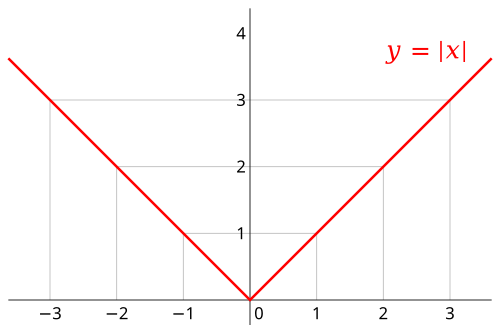
\includegraphics[width=4cm]{abs}
        \caption{The graph of the absolute value function $f(x) = |x|$.}
    \end{figure}
    -- Nếu khả vi không đạt tại 1 điểm bên trong của khoảng, kết luận của định lý Rolle có thể không đúng. Xét hàm giá trị tuyệt đối $f(x) = |x|$, $x\in[-1,1]$. Khi đó $f(-1) = f(1)$, nhưng không có $c\in(-1,1$ nào mà $f'(c) = 0$. Điều này là do hàm đó, mặc dù liên tục, nhưng không khả vi tại $x = 0$, nhưng không đạt được giá trị 0. Không thể áp dụng định lý cho hàm này vì nó không thỏa mãn điều kiện là hàm phải khả vi với mọi $x$ trong khoảng mở. Tuy nhiên, khi yêu cầu khả vi bị loại bỏ khỏi định lý Rolle, $f$ vẫn sẽ có 1 số tới hạn trong khoảng mở $(a,b)$, nhưng nó có thể không tạo ra 1 tiếp tuyến ngang (như trong trường hợp giá trị tuyệt đối được biểu diễn trong đồ thị).
\end{example}

\paragraph*{Functions with zero derivative -- Các hàm số có đạo hàm bằng $0$.} Rolle's theorem implies that:

\begin{theorem}
    A differentiable function whose derivative is 0 in an interval is constant in this interval.
\end{theorem}

\begin{dinhly}
    1 hàm số khả vi có đạo hàm bằng 0 trên 1 khoảng thì là 1 hàm số hằng số trong khoảng đó.    
\end{dinhly}

\begin{proof}
    Indeed, if $a,b$ are 2 points in an interval where a function $f$ is differentiable, then the function
    \begin{equation*}
        g(x) = f(x) - f(a) - \frac{f(b) - f(a)}{b - a}(x - a)
    \end{equation*}
    satisfies the hypotheses of Rolle's theorem on the interval $[a,b]$. If the derivative of $f$ is zero everywhere, the derivative of $g$ is $g'(x) = \frac{f(b) - f(a)}{b - a}$, \& Rolle's theorem implies that there is $c\in(a,b)$ s.t. $0 = g'(c) = \frac{f(b) - f(a)}{b - a}(x - a)$. Hence, $f(a) = f(b)$ for every $a,b$, \& the function $f$ is constant.
\end{proof}

\begin{dinhly}
    1 hàm số khả vi có đạo hàm bằng 0 trên 1 khoảng thì là 1 hàm số hằng số trong khoảng đó.
\end{dinhly}

\begin{proof}
    Thật vậy, nếu $a,b$ là 2 điểm trong 1 khoảng mà hàm $f$ có thể vi phân, thì hàm
    \begin{equation*}
        g(x) = f(x) - f(a) - \frac{f(b) - f(a)}{b - a}(x - a)
    \end{equation*}
    thỏa mãn các giả thuyết của định lý Rolle trên khoảng $[a,b]$. Nếu đạo hàm của $f$ bằng 0 ở mọi nơi, thì đạo hàm của $g$ là $g'(x) = \frac{f(b) - f(a)}{b - a}$, \& Định lý Rolle ngụ ý rằng có $c\in(a,b)$ s.t. $0 = g'(c) = \frac{f(b) - f(a)}{b - a}(x - a)$. Do đó, $f(a) = f(b)$ với mọi $a,b$, \& hàm $f$ là hằng số.
\end{proof}

%------------------------------------------------------------------------------%

\subsection{Generalization of Rolle's theorem -- Tổng quát hóa của định lý Rolle}

\begin{theorem}
    Consider a real-valued, continuous function $f$ on a closed interval $[a,b]$ with $f(a) = f(b)$. if for every $x$ in the open interval $(a,b)$ the right-hand- \& the left-hand limits
    \begin{equation*}
        f'(x^+)\coloneqq\lim_{h\to0^+} \frac{f(x + h) - f(x)}{h},\ f'(x^-)\coloneqq\lim_{h\to0^-} \frac{f(x + h) - f(x)}{h}
    \end{equation*}
    exist in the extended real line $\overline{\mathbb{R}}\coloneqq[-\infty,\infty]$, then there is some number $c\in(a,b)$ s.t. 1 of the 2 limits $f'(c^+),f'(c^-)$ is $\ge0$ \& the other is $\le0$ (in the extended real line). If the right- \& left-hand limits agree for every $x$, then they agree in particular for $c$, hence the derivative of $f$ exists at $c$ \& is equal to zero, i.e., $f'(c) = 0$.
\end{theorem}

\begin{proof}[Proof]
    Since the proof for the standard version of Rolle's theorem \& the generalization are very similar, we prove the generalization. The idea of the proof is to argue that if $f(a) = f(b)$, then $f$ must attain either a maximum or a minimum somewhere between $a$ \& $b$, say at $c$, \& the function must change from increasing to decreasing (or the other way around) at $c$. In particular, if the derivative exists, it must be zero at $c$.
    
    By assumption, $f$ is continuous on $[a,b]$, \& by the extreme value theorem attains both its maximum \& its minimum in $[a,b]$. If these are both attained at the endpoints of $[a,b]$, then $f$ is constant on $[a,b]$ \& so the derivative of $f$ is zero at every point in $(a,b)$.
    
    Suppose then that the maximum is obtained at an interior point $c$ of $(a,b)$ (the argument for the minimum is very similar, just consider $-f$). We shall examine the above right- \& left-hand limits separately.
    
    For a real $h$ s.t. $c + h\in[a,b]$, the value $f(c + h)\le f(c)$ because $f$ attains its maximum at $c$. Therefore, for every $h > 0$, $\frac{f(c + h) - f(c)}{h}\le0$, hence
    \begin{equation*}
        f'(c^+)\coloneqq\lim_{h\to0^+} \frac{f(c + h) - f(c)}{h}\le0,
    \end{equation*}
    where the limit exists by assumption, it may be minus infinity. Similarly, for every $h < 0$, the inequality turns around because the denominator is now negative \& we get $\frac{f(c + h) - f(c)}{h}\ge0$, hence
    \begin{equation*}
        f'(c^-)\coloneqq\lim_{h\to0^-} \frac{f(c + h) - f(c)}{h}\ge0,
    \end{equation*}
    where the limit might be plus infinity.
    
    Finally, when the above right- \& left-hand limits agree (in particular when $f$ is differentiable), then the derivative of $f$ at $c$ must be zero. (Alternatively, we can apply Fermat's stationary point theorem directly.)
\end{proof}

\begin{dinhly}
    Xét 1 hàm liên tục giá trị thực $f$ trên 1 khoảng đóng $[a,b]$ với $f(a) = f(b)$. nếu với mọi $x$ trong khoảng mở $(a,b)$ các giới hạn bên phải \& bên trái
    \begin{equation*}
        f'(x^+)\coloneqq\lim_{h\to0^+} \frac{f(x + h) - f(x)}{h},\ f'(x^-)\coloneqq\lim_{h\to0^-} \frac{f(x + h) - f(x)}{h}
    \end{equation*}
    tồn tại trên trục số thực mở rộng $\overline{\mathbb{R}}\coloneqq[-\infty,\infty]$, thì tồn tại 1 số $c\in(a,b)$ s.t. 1 trong 2 giới hạn $f'(c^+),f'(c^-)$ là $\ge0$ \& giới hạn còn lại là $\le0$ (trên trục số thực mở rộng). Nếu các giới hạn bên phải \& bên trái đồng ý với mọi $x$, thì chúng đồng ý đặc biệt với $c$, do đó đạo hàm của $f$ tồn tại tại $c$ \& bằng không, tức là $f'(c) = 0$.
\end{dinhly}

\begin{proof}
    Vì bằng chứng cho phiên bản chuẩn của định lý Rolle \& tổng quát hóa rất giống nhau, chúng tôi chứng minh tổng quát hóa. Ý tưởng của bằng chứng là lập luận rằng nếu $f(a) = f(b)$, thì $f$ phải đạt cực đại hoặc cực tiểu ở đâu đó giữa $a$ \& $b$, chẳng hạn tại $c$, \& hàm phải thay đổi từ tăng sang giảm (hoặc ngược lại) tại $c$. Đặc biệt, nếu đạo hàm tồn tại, thì nó phải bằng không tại $c$.
    
    Theo giả thiết, $f$ liên tục trên $[a,b]$, \& theo định lý giá trị cực trị đạt cả cực đại \& cực tiểu tại $[a,b]$. Nếu cả hai đều đạt được tại các điểm cuối của $[a,b]$, thì $f$ là hằng số trên $[a,b]$ \& do đó đạo hàm của $f$ bằng không tại mọi điểm trong $(a,b)$.
    
    Giả sử rằng giá trị cực đại đạt được tại 1 điểm bên trong $c$ của $(a,b)$ (lập luận cho giá trị cực tiểu rất giống, chỉ cần xét $-f$). Chúng ta sẽ xem xét riêng các giới hạn bên phải \& bên trái ở trên.
    
    Đối với 1 $h$ s.t. $c + h\in[a,b]$ thực, giá trị $f(c + h)\le f(c)$ vì $f$ đạt giá trị cực đại tại $c$. Do đó, với mọi $h > 0$, $\frac{f(c + h) - f(c)}{h}\le0$, do đó
    \begin{equation*}
        f'(c^+)\coloneqq\lim_{h\to0^+} \frac{f(c + h) - f(c)}{h}\le0,
    \end{equation*}
    trong đó giới hạn tồn tại theo giả thiết, nó có thể là âm vô cực. Tương tự, với mọi $h < 0$, bất đẳng thức đảo ngược vì mẫu số bây giờ là số âm \& ta có $\frac{f(c + h) - f(c)}{h}\ge0$, do đó
    \begin{equation*}
        f'(c^-)\coloneqq\lim_{h\to0^-} \frac{f(c + h) - f(c)}{h}\ge0,
    \end{equation*}
    trong đó giới hạn có thể là cộng vô cực.
    
    Cuối cùng, khi các giới hạn bên phải \& bên trái ở trên bằng nhau (đặc biệt khi $f$ khả vi), thì đạo hàm của $f$ tại $c$ phải bằng không. (Ngoài ra, ta có thể áp dụng trực tiếp định lý điểm dừng của Fermat.)
\end{proof}

\begin{remark}
    \item(a) If $f$ is convex or concave, then the right- \& left-hand derivatives exist at every inner point, hence the above limits exist \& are real numbers.
    
    -- Nếu $f$ lồi hoặc lõm thì đạo hàm phải \& trái tồn tại tại mọi điểm bên trong, do đó các giới hạn trên tồn tại \& là số thực.
    \item(b) This generalized version of the theorem is sufficient to prove \href{https://en.wikipedia.org/wiki/Convex_function}{convexity} when the 1-sided derivatives are \href{https://en.wikipedia.org/wiki/Monotonically_increasing}{monotonically increasing}: $f'(x^-)\le f'(x^+)\le f'(y^-)$, $x < y$.
    
    -- Phiên bản tổng quát của định lý này đủ để chứng minh tính lồi khi đạo hàm 1 phía tăng đơn điệu: $f'(x^-)\le f'(x^+)\le f'(y^-)$, $x < y$.
\end{remark}

%------------------------------------------------------------------------------%

\subsection{Generalization of Rolle's theorem to higher derivatives -- Tổng quát hoá của định lý Rolle cho các đạo hàm cấp cao}
We can also generalize Rolle's theorem by requiring that $f$ has more points with equal values \& greater regularity. Specifically:

\begin{theorem}
    Suppose that
    \item(i) the function $f$ is $n - 1$ times continuously differentiable on the closed interval $[a,b]$ \& the $n$th derivative exists on the open interval $(a,b)$, \&
    \item(ii) there are $n$ intervals given by $a_1 < b_1\le a_2 < b_2\le\cdots\le a_n < b_n$ in $[a,b]$ s.t. $f(a_i) = f(b_i)$, $\forall i\in[n]$.
    
    Then there is a number $c\in(a,b)$ s.t. the $n$th derivative of $f$ at $c$ is zero.
\end{theorem}

\begin{proof}[Proof]
    The proof uses mathematical induction. The case $n == 1$ is simply the standard version of Rolle's theorem. For $n > 1$, take as the induction hypothesis that the generalization is true for $n - 1$. We want to prove it for $n$. Assume the function $f$ satisfies the hypotheses of the theorem. By the standard version of Rolle's theorem, for every $i\in[n]$, there exists a $c_i\in(a_i,b_i)$ s.t. $f'(c_i) = 0$. Hence, the 1st derivative satisfies the assumptions on the $n - 1$ closed intervals $[c_1,c_2],\ldots,[c_{n-1},c_n]$. By the induction hypothesis, there is a $c$ s.t. the $(n - 1)$st derivative of $f'$ at $c$ is 0.
\end{proof}

\begin{dinhly}
    Giả sử rằng
    \item(i) hàm $f$ có đạo hàm liên tục $n - 1$ lần trên khoảng đóng $[a,b]$ \& đạo hàm bậc $n$ tồn tại trên khoảng mở $(a,b)$, \&
    \item(ii) có $n$ khoảng được cho bởi $a_1 < b_1\le a_2 < b_2\le\cdots\le a_n < b_n$ trong $[a,b]$ s.t. $f(a_i) = f(b_i)$, $\forall i\in[n]$.
    
    Khi đó có 1 số $c\in(a,b)$ s.t. đạo hàm bậc $n$ của $f$ tại $c$ bằng không.
\end{dinhly}

\begin{proof}
    Chứng minh sử dụng phép quy nạp toán học. Trường hợp $n == 1$ chỉ đơn giản là phiên bản chuẩn của định lý Rolle. Với $n > 1$, lấy giả thuyết quy nạp rằng phép tổng quát đúng với $n - 1$. Chúng ta muốn chứng minh nó với $n$. Giả sử hàm $f$ thỏa mãn các giả thuyết của định lý. Theo phiên bản chuẩn của định lý Rolle, với mọi $i\in[n]$, tồn tại 1 $c_i\in(a_i,b_i)$ s.t. $f'(c_i) = 0$. Do đó, đạo hàm bậc 1 thỏa mãn các giả thiết trên các khoảng đóng $n - 1$ $[c_1,c_2],\ldots,[c_{n-1},c_n]$. Theo giả thuyết quy nạp, tồn tại 1 $c$ s.t. đạo hàm bậc $(n - 1)$ của $f'$ tại $c$ bằng 0.
\end{proof}
The requirements concerning the $n$th derivative of $f$ can be weakened as in the generalization above, giving the corresponding (possibly weaker) assertions for the right- \& left-hand limits defined above with $f^{(n-1)}$ in place of $f$.

-- Các yêu cầu liên quan đến đạo hàm bậc $n$ của $f$ có thể bị yếu đi như trong khái quát ở trên, đưa ra các khẳng định tương ứng (có thể yếu hơn) cho giới hạn bên phải \& bên trái được xác định ở trên với $f^{(n-1)}$ thay cho $f$.

Particularly, this version of the theorem asserts that if a function differentiable enough times has $n$ roots (so they have the same value, i.e. 0), then there is an internal point where $f^{(n-1)}$ vanishes.

-- Đặc biệt, phiên bản định lý này khẳng định rằng nếu 1 hàm số khả vi đủ số lần có $n$ nghiệm (do đó chúng có cùng giá trị, tức là 0), thì có 1 điểm bên trong mà tại đó $f^{(n-1)}$ biến mất.

%------------------------------------------------------------------------------%

\subsection{Generalizations of Rolle's theorem to other fields -- Các tổng quát hóa của định lý Rolle cho các lĩnh vực khác}
Rolle's theorem is a property of differentiable functions over the real numbers, which are an \href{https://en.wikipedia.org/wiki/Ordered_field}{ordered field}. As such, it does not generalize to other fields, but the following corollary does: if a real polynomial factors (has all of its roots) over the real numbers, then its derivative does as well. One may call this property of a field {\it Rolle's property}. More general fields do not always have differentiable functions, but they do always have polynomials, which can be symbolically differentiated. Similarly, more general fields may not have an order, but one has a notion of a root of a polynomial lying in a field.

-- Định lý Rolle là 1 tính chất của các hàm khả vi trên các số thực, là 1 trường có thứ tự. Do đó, nó không tổng quát hóa cho các trường khác, nhưng hệ quả sau đây thì có: nếu 1 đa thức thực phân tích nhân tử (có tất cả các nghiệm của nó) trên các số thực, thì đạo hàm của nó cũng vậy. Người ta có thể gọi tính chất này của 1 trường là {\it tính chất Rolle}. Các trường tổng quát hơn không phải lúc nào cũng có các hàm khả vi, nhưng chúng luôn có các đa thức, có thể được phân biệt theo ký hiệu. Tương tự như vậy, các trường tổng quát hơn có thể không có thứ tự, nhưng người ta có khái niệm về 1 nghiệm của 1 đa thức nằm trong 1 trường.

Thus Rolle's theorem shows that the real numbers have Rolle's property. Any algebraically closed field e.g. the complex numbers has Rolle's property. However, the rational numbers do not -- e.g., $x^3 - x = x(x - 1)(x + 1)$ factors over the rationals, but its derivative $3x^2 - 1 = 3\left(x - \frac{1}{\sqrt{3}}\right)\left(x + \frac{1}{\sqrt{3}}\right)$ does not. The question of which fields satisfy Rolle's property was raised in [Kaplansky1972]. For finite fields, the answer is that only $\mathbb{F}^2,\mathbb{F}^4$ have Rolle's property. For a complex version, see \href{https://en.wikipedia.org/wiki/Voorhoeve_index}{Wikipedia{\tt/}Voorhoeve index}.

-- Do đó, định lý Rolle chứng tỏ rằng các số thực có tính chất Rolle. Bất kỳ trường đại số đóng nào, ví dụ như các số phức, đều có tính chất Rolle. Tuy nhiên, các số hữu tỉ không -- ví dụ, $x^3 - x = x(x - 1)(x + 1)$ phân tích thành các số hữu tỉ, nhưng đạo hàm của nó $3x^2 - 1 = 3\left(x - \frac{1}{\sqrt{3}}\right)\left(x + \frac{1}{\sqrt{3}}\right)$ thì không. Câu hỏi về trường nào thỏa mãn tính chất Rolle đã được nêu ra trong [Kaplansky1972]. Đối với các trường hữu hạn, câu trả lời là chỉ $\mathbb{F}^2,\mathbb{F}^4$ có tính chất Rolle. Đối với phiên bản phức, hãy xem chỉ số Voorhoeve.

%------------------------------------------------------------------------------%

\section{Lagrange Theorem -- Định Lý Lagrange}

\begin{dinhly}[Lagrange]
    Cho $f(x)$ xác định \& liên tục trên $[a,b]$, khả vi trên $(a,b)$. Khi đó tồn tại $c\in(a,b)$ sao cho $f'(c) = \dfrac{f(b) - f(a)}{b - a}$.
\end{dinhly}

%------------------------------------------------------------------------------%

\section{Cauchy Theorem -- Định Lý Cauchy}

\begin{dinhly}[Cauchy]
    Cho $f(x),g(x)$ liên tục trên $[a,b]$, khả vi trên $(a,b)$, $g'(x)\ne0$, $\forall x\in(a,b)$. Khi đó tồn tại $c\in(a,b)$ sao cho $\dfrac{f(b) - f(a)}{g(b) - g(a)} = \dfrac{f'(c)}{g'(c)}$.
\end{dinhly}

%------------------------------------------------------------------------------%

\section{Darboux Theorem -- Định Lý Darboux}

\begin{dinhly}[Darboux]
    Nếu hàm số $f(x)$ khả vi trên $(a,b)$, $\alpha,\beta\in(a,b)$ thì $f'(x)$ nhận mọi giá trị trung gian giữa $f'(\alpha)$ \& $f'(\beta)$.
\end{dinhly}
I.e.,
\begin{equation*}
    (\min\{f'(\alpha),f'(\beta)\},\max\{f'(\alpha),f'(\beta)\})\subset f'((a,b)),\ \forall f(x)\mbox{ differentiable on }(a,b),\ \forall\alpha,\beta\in(a,b).
\end{equation*}

\begin{baitoan}[\cite{Quoc_Long_Dat_Nam_VMC}, 3.14., p. 152]
    Cho $f:\left[-\frac{\pi}{2},\frac{\pi}{2}\right]\to[-1,1]$ là 1 hàm khả vi có đạo hàm liên tục \& không âm ($f'\ge0$). Chứng minh tồn tại $x_0\in\left(-\frac{\pi}{2},\frac{\pi}{2}\right)$ sao cho $(f(x_0))^2 + (f'(x_0))^2\le1$.
\end{baitoan}




\begin{baitoan}[\cite{TLCT_BT_dai_so_giai_tich_11}, 15., p. 50]
	Cho $a,b,c\in\mathbb{R},2a + 3b + 6c = 0$. Chứng minh phương trình $ax^2 + bx + c = 0$ có ít nhất 1 nghiệm thuộc $(0,1)$.
\end{baitoan}

\begin{baitoan}[\cite{TLCT_BT_dai_so_giai_tich_11}, 16., p. 50]
	Cho $f(x) = x(x - 1)(x - 2)(x - 3)(x - 4)(x - 5)(x - 6)$. Đếm số nghiệm của phương trình $f'(x) = 0$.
\end{baitoan}

\begin{baitoan}[\cite{TLCT_BT_dai_so_giai_tich_11}, 17., p. 51]
	Xét hàm số $f(x)$ liên tục trên đoạn $[a,b]$ có đạo hàm trên $(a,b)$. Giả sử phương trình $f(x) = 0$ có đúng 2 nghiệm $x_1,x_2$ với $x_1\ne x_2$. Chứng minh phương trình $f'(x) = 0$ có nghiệm, hơn nữa biểu thức $f'(x)$ phải đổi dấu.
\end{baitoan}

\begin{baitoan}[\cite{TLCT_BT_dai_so_giai_tich_11}, 18., p. 51]
	Chứng minh $2(\sqrt{n + 1} - \sqrt{n}) < \frac{1}{\sqrt{n}} < 2(\sqrt{n} - \sqrt{n - 1})$, $\forall n\in\mathbb{N}^\star$.
\end{baitoan}

\begin{baitoan}[\cite{TLCT_BT_dai_so_giai_tich_11}, 19., p. 51]
	Cho $0 < a < b$ \& $f$ là 1 hàm liên tục trên $[a,b]$, có đạo hàm trên $(a,b)$. Chứng minh tồn tại $c\in(a,b)$ thỏa $\dfrac{af(b) - bf(a)}{a - b} = f(c) - f'(c)$.
\end{baitoan}

\begin{baitoan}[\cite{TLCT_BT_dai_so_giai_tich_11}, 20., p. 51]
	Tính giới hạn: (a) $\lim_{x\to0} \dfrac{\tan x - \sin x}{x^3}$. (b) $\lim_{x\to0} \dfrac{\sqrt[m]{1 + x} - 1}{\sqrt[n]{1 + x} - 1}$. (c) $\lim_{x\to0} \dfrac{1 - \cos x}{x\sin x}$.
\end{baitoan}

\begin{baitoan}[\cite{TLCT_BT_dai_so_giai_tich_11}, 21., p. 51]
	Tính giới hạn: (a) $\lim_{x\to1} \left(\dfrac{1}{x - 1} - \dfrac{1}{\ln x}\right)$. (b) $\lim_{x\to0} (1 + x)^{\cot x}$.
\end{baitoan}

%------------------------------------------------------------------------------%

\chapter{2nd-Order Derivative -- Đạo Hàm Cấp 2}
\minitoc

%------------------------------------------------------------------------------%

\chapter{Vi Phân \& Đạo Hàm Cấp Cao}
\minitoc

\begin{baitoan}[\cite{TLCT_BT_dai_so_giai_tich_11}, 22., p. 51]
	Tính vi phân của hàm số: (a) $y = \sqrt{x^2 + a^2}$. (b) $y = x\sin x$. (c) $y = x^2 + \sin^2x$. (d) $y = e^x\ln x$.
\end{baitoan}

\begin{baitoan}[\cite{TLCT_BT_dai_so_giai_tich_11}, 23., p. 51]
	Làm tròn đến hàng phần nghìn: (a) $\dfrac{1}{0.9995}$. (b) $\ln1.001$. (c) $\cos61^\circ$.
\end{baitoan}

\begin{baitoan}[\cite{TLCT_BT_dai_so_giai_tich_11}, 24., p. 51]
	Chứng minh nếu $f,g$ là 2 hàm số có đạo hàm đến cấp 2 thì $fg$ cũng có đạo hàm đến cấp 2 \& có công thức $(f(x)g(x))'' = f''(x)g(x) + 2f'(x)g'(x) + g''(x)$.
\end{baitoan}

\begin{baitoan}[\cite{TLCT_BT_dai_so_giai_tich_11}, 25., p. 51]
	Tính đạo hàm: (a) $f(x) = x^4 - \cos2x$, tính $f^{(4)}(x)$. (b) $f(x) = \cos^2x$, tính $f^{(5)}(x)$. (c) $f(x) = (x + 10)^6$, tính $f^{(n)}(x)$.
\end{baitoan}

\begin{baitoan}[\cite{TLCT_BT_dai_so_giai_tich_11}, 26., p. 52]
	Vận tốc của 1 chất điểm chuyển động được biểu thị bởi công thức $v(t) = 8t + 3t^2$, với $t > 0$, $t$ được tính bằng giây {\rm s} \& $v(t)$ tính bằng {\rm m{\tt/}s}. Tính gia tốc của chất điểm: (a) Lúc $t = 4$. (b) Lúc vận tốc chuyển động bằng $11$.
\end{baitoan}

\begin{baitoan}[\cite{TLCT_BT_dai_so_giai_tich_11}, 27., p. 52]
	Chứng minh $\forall n\ge1$: (a) Nếu $f(x) = \frac{1}{x}$ thì $f^{(n)}(x) = \dfrac{(-1)^nn!}{x^{n+1}}$. (b) Nếu $f(x) = \cos x$ thì $f^{(n)}(x) = \cos\left(x + \frac{n\pi}{2}\right)$.
\end{baitoan}

\begin{baitoan}[\cite{TLCT_BT_dai_so_giai_tich_11}, 28., p. 52]
	Cho $f(x) = \sqrt{x}$. Tính $f^{(n)}(x)$.
\end{baitoan}

%------------------------------------------------------------------------------%

\section{Miscellaneous}

\begin{baitoan}[\cite{TLCT_BT_dai_so_giai_tich_11}, 29., p. 52]
	Tính $f'(x)$ với
	\begin{equation}
		f(x) = \left\{\begin{split}
			&2x + 1&&\mbox{if } x < 1,\\
			&x^2 + 1&&\mbox{if } 1\le x\le2,\\
			&x^3 - x^2 - 4x + 10&&\mbox{if } x > 2.
		\end{split}\right.
	\end{equation}
\end{baitoan}

\begin{baitoan}[\cite{TLCT_BT_dai_so_giai_tich_11}, 30., p. 52]
	Tính $f'(x) + f(x) + 2$ nếu $f(x) = x\sin2x$.
\end{baitoan}

\begin{baitoan}[\cite{TLCT_BT_dai_so_giai_tich_11}, 31., p. 52]
	Chứng minh nếu $f(x) = 3e^{x^2}$ thì $f'(x) - 2xf(x) + \frac{1}{3}f(0) - f'(0) = 1$.
\end{baitoan}

\begin{baitoan}[\cite{TLCT_BT_dai_so_giai_tich_11}, 32., p. 52]
	Viết phương trình tiếp tuyến của đường cong $y = 4x - x^2$ tại các điểm mà đường cong cắt trục hoành.
\end{baitoan}

\begin{baitoan}[\cite{TLCT_BT_dai_so_giai_tich_11}, 33., p. 52]
	Cho đa thức bậc 4 $P(x)$ thỏa mãn điều kiện $P(x)\ge0$, $\forall x\in\mathbb{R}$. Chứng minh $P(x) + P'(x) + P''(x) + P^{(3)}(x) + P^{(4)}(x)\ge0$, $\forall x\in\mathbb{R}$.
\end{baitoan}

\begin{baitoan}[\cite{TLCT_BT_dai_so_giai_tich_11}, 34., p. 53]
	Áp dụng định lý Rolle cho hàm số $f(x) = e^xP(x)$ để chứng minh nếu đa thức $P(x)$ bậc $n$ có $n$ nghiệm thực phân biệt thì đa thức $P(x) + P'(x)$ cũng có $n$ nghiệm thực phân biệt.
\end{baitoan}

\begin{baitoan}[\cite{TLCT_BT_dai_so_giai_tich_11}, 35., p. 53]
	Cho hàm số $f(x)$ khả vi trên đoạn $[0,1]$ \& $f'(0)f'(1) < 0$. Chứng minh tồn tại $c\in(0,1)$ thỏa $f'(c) = 0$.
\end{baitoan}

\begin{baitoan}[\cite{TLCT_BT_dai_so_giai_tich_11}, 36., p. 53]
	Giả sử $f(x)$ là 1 hàm số lẻ \& khả vi trên $\mathbb{R}$. Chứng minh $f'(x)$ là 1 hàm số chẵn.
\end{baitoan}

\begin{baitoan}[\cite{TLCT_BT_dai_so_giai_tich_11}, 37., p. 53]
	Tính đạo hàm cấp $100$ của hàm số $f(x) = \dfrac{x}{x^2 - 1}$.
\end{baitoan}

\begin{baitoan}[\cite{TLCT_BT_dai_so_giai_tich_11}, 38., p. 53]
	Tính giới hạn: (a) $\lim_{x\to0} \cos^{\frac{1}{2x^2}} x$. (b) $\lim_{x\to0} \cos^{\frac{5}{x}} 3x$.
\end{baitoan}

\begin{baitoan}[\cite{TLCT_BT_dai_so_giai_tich_11}, 39., p. 53]
	Chứng minh: (a) {\rm (Phương trình dao động điều hòa)} Nếu $y = A\sin(\omega t + \varphi) + B\cos(\omega t + \varphi)$ với $A,B,\omega,\varphi$ là 4 hằng số thì $y'' + \omega^2y = 0$. (b) Nếu $y = \sqrt{2x - x^2}$ thì $y^3y'' + 1 = 0$.
\end{baitoan}

\begin{baitoan}[\cite{TLCT_BT_dai_so_giai_tich_11}, 40., p. 53, công thức Newton--Leibnitz]
	Cho $f,g$ là 2 hàm số có đạo hàm đến cấp $n$, chứng minh công thức: $(f(x)g(x))^{(n)} = \sum_{k=0}^n C_n^kf^{(k)}(x)g^{(n-k)}(x)$.
\end{baitoan}

\begin{baitoan}[\cite{TLCT_BT_dai_so_giai_tich_11}, 41., p. 53]
	Cho hàm số $f(x) = \dfrac{x}{x^2 + 1}$. Tính $f^{(100)}(0),f^{(101)}(0)$.
\end{baitoan}

%------------------------------------------------------------------------------%

\begin{baitoan}[\cite{VMS_VMC2023}, p. 36, 4.1, VNUHCM UIT]
	Cho hàm $f\in C^2(\mathbb{R})$ thỏa $f(0) = 2$, $f'(0) = -2$, $f(1) = 1$. Chứng minh tồn tại $c\in(0,1)$ thỏa $f(c)f'(c) + f''(c) = 0$.
\end{baitoan}

\begin{baitoan}[\cite{VMS_VMC2023}, p. 37, 4.2, ĐH Đồng Tháp]
	Cho $f$ khả vi trên $(a,\infty)$, $\forall a\in(0,\infty)$ \& $\lim_{x\to\infty} f'(x) = 0$. Chứng minh $\lim_{x\to\infty} \dfrac{f(x)}{x} = 0$.
\end{baitoan}

\begin{baitoan}[\cite{VMS_VMC2023}, p. 37, 4.3, ĐH Đồng Tháp]
	Cho $f$ là hàm số có đạo hàm $f'$ đồng biến trên $[0,2]$ \& $f(0) = -1,f(2) = 1$. Chứng minh tồn tại $a,b,c\in[0,2]$ thỏa $f'(a)f'(b)f'(c) = 1$.
\end{baitoan}

\begin{baitoan}[\cite{VMS_VMC2023}, p. 37, 4.4, ĐHGTVT]
	Cho $f\in C^\infty(\mathbb{R})$ thỏa $f^{(n)}(0) = 0$, $\forall n\in\mathbb{N}$ \& $f^{(n)}(x)x\ge0$, $\forall k\in\mathbb{N}^\star$, $\forall x\in(0,\infty)$. Chứng minh $f(x) = 0$, $\forall x\in(0,\infty)$.	 
\end{baitoan}

\begin{baitoan}[\cite{VMS_VMC2023}, p. 37, 4.5, ĐH Hùng Vương, Phú Thọ]
	Giả sử hàm $f\in C([1,2023])$, khả vi trong khoảng $(1,2023)$, \& $f(2023) = 0$. Chứng minh tồn tại $c\in(1,2023)$ thỏa
	\begin{equation*}
		f'(c) = \frac{2024 - 2023c}{1 - c}f(c).
	\end{equation*}
\end{baitoan}

\begin{baitoan}[\cite{VMS_VMC2023}, p. 37, 4.6, ĐHKH Thái Nguyên]
	Giả sử $f(x)\in C^\infty([-1,1])$, $f^{(n)}(0) = 0$, $\forall n\in\mathbb{N}$, \& tồn tại $\alpha\in(0,1)$ thỏa $\sup_{x\in[-1,1]} |f^{(n)}(x)|\le\alpha^nn!$, $\forall n\in\mathbb{N}$. Chứng minh $f(x)\equiv0$ trên đoạn $[-1,1]$.
\end{baitoan}

\begin{baitoan}[\cite{VMS_VMC2023}, p. 37, 4.7, ĐHSPHN2]
	Cho $f\in C([a,b])$ khả vi trên $(a,b)$. Giả sử $f'(x) > 0$, $\forall x\in(a,b)$. Chứng minh $\forall x_1,x_2\in\mathbb{R}$ thỏa $a\le x_1 < x_2\le b$ \& $f(x_1)f(x_2) > 0$ thì luôn tồn tại $c\in(x_1,x_2)$ thỏa
	\begin{equation*}
		\frac{x_1f(x_2) - x_2f(x_1)}{f(x_2) - f(x_1)} = c - \frac{f(c)}{f'(c)}.
	\end{equation*}
\end{baitoan}

\begin{baitoan}[\cite{VMS_VMC2024}, p. 33, 3.1, VNUHCM UIT]
	Cho $f$ là hàm số thực trên $(0,\infty)$. Giả sử
	\begin{equation*}
		f(x^\alpha) = f(x)\sin^2\alpha + f(1)\cos^2\alpha,\ \forall x\in(0,\infty),\ \forall\alpha\in\mathbb{R}.
	\end{equation*}
	Chứng minh $f$ khả vi tại $1$.
\end{baitoan}

\begin{baitoan}[\cite{VMS_VMC2024}, p. 34, 3.2, ĐH Đồng Tháp]
	(a) Chứng minh với mỗi $n\in\mathbb{N}^\star$, phương trình $2x = \sqrt{x + n} + \sqrt{x + n + 1}$ có nghiệm dương duy nhất, ký hiệu là $x_n$. (b) Tính $a\coloneqq\lim_{n\to\infty} \dfrac{x_n}{\sqrt{n}},b\coloneqq \lim_{n\to\infty} x_n - a\sqrt{n}$.
\end{baitoan}

\begin{baitoan}[\cite{VMS_VMC2024}, p. 34, 3.3, ĐH Đồng Tháp]
	Cho
	\begin{equation*}
		f(x) = \left\{\begin{split}
			&x^2\left|\cos\frac{\pi}{x}\right|&&\mbox{if } x\ne0,\\
			&0&&\mbox{if } x = 0.
		\end{split}\right.
	\end{equation*}
	Chứng minh $f$ khả vi tại $0$ nhưng $f$ không khả vi tại các điểm $x_n\coloneqq\dfrac{2}{2n + 1}$ với $n\in\mathbb{Z}$.
\end{baitoan}

\begin{baitoan}[\cite{VMS_VMC2024}, p. 34, 3.4, ĐH Đồng Tháp]
	Giả sử $f$ khả vi liên tục trên $(0,\infty)$, $f(0) = 1$. Chứng minh nếu $|f(x)|\le e^{-x}$, $\forall x\ge0$ thì tồn tại $x_0 > 0$ để $f'(x_0) = -e^{-x_0}$.
\end{baitoan}

\begin{baitoan}[\cite{VMS_VMC2024}, p. 34, 3.5, ĐHGTVT]
	Cho $a\in\mathbb{R}$, $b\in(0,\infty)$. Hàm $f$ xác định trên $[-1,1]$, được cho bởi
	\begin{equation*}
		f(x) = \left\{\begin{split}
			&x^a\sin x^{-b}&&\mbox{if } x\ne0,\\
			&0&&\mbox{if } x = 0.
		\end{split}\right.
	\end{equation*}
	(a) Tìm tất cả các giá trị của $a$ để hàm $f$ liên tục trên $[-1,1]$. (b) Tìm tất cả các giá trị của $a$ để tồn tại $f'(0)$. (c) Tìm điều kiện của $a,b$ để tồn tại $f''(0)$.
\end{baitoan}

\begin{baitoan}[\cite{VMS_VMC2024}, p. 35, 3.7, HUS]
	Cho $f:\mathbb{R}\to\mathbb{R}$ là hàm số được xác định bởi công thức
	\begin{equation*}
		f(x) = \left\{\begin{split}
			&x^2 + a&&\mbox{if } x\le0,\\
			&be^x + x&&\mbox{if } x > 0,
		\end{split}\right.
	\end{equation*}
	với $a,b\in\mathbb{R}$: tham số. Xác định $a,b$ để $f$ có nguyên hàm trên $\mathbb{R}$.
\end{baitoan}

\begin{baitoan}[\cite{VMS_VMC2024}, p. 35, 3.8, ĐH Vinh]
	Cho hàm $f\in C(\mathbb{R},\mathbb{R})$ thỏa $f_{2024}(x) = x$, $\forall x\in\mathbb{R}$ với
	\begin{equation*}
		\left\{\begin{split}
			f_{n+1}(x) &= f(f_n(x)),\ \forall x\in\mathbb{R},\,\forall n\in\mathbb{N}^\star,\\
			f_1(x) &= f(x),\ \forall x\in\mathbb{R}
		\end{split}\right.
	\end{equation*}
	Chứng minh $f_2(x) = x$, $\forall x\in\mathbb{R}$.
\end{baitoan}

\begin{baitoan}[\cite{VMS_VMC2024}, p. 35, 3.9, ĐH Vinh]
	Cho hàm
	\begin{equation*}
		f(x) = \left(\frac{2023^x + 2024^x}{2}\right)^{\frac{1}{x}},\ x > 0.
	\end{equation*}
	(a) Tìm $\lim_{x\to0^+} f(x)$. (b) Chứng minh $f$ là hàm số đơn điệu tăng trên $(0,+\infty)$.
\end{baitoan}

\begin{baitoan}[\cite{VMS_VMC2024}, p. 36, 4.1, HCMUT]
	(a) Cho $f\in C^3(\mathbb{R},[0,+\infty))$ thỏa $\max_{x\in\mathbb{R}} |f'''(x)|\le1$. Chứng minh
	\begin{equation*}
		f''(x)\ge-\sqrt[3]{\frac{3}{2}f(x)},\ \forall x\in\mathbb{R}.
	\end{equation*}
	(b) Tìm tất cả các hàm số $f$ thỏa mãn điều kiện của (a) thỏa
	\begin{equation*}
		f''(x) = -\sqrt[3]{\frac{3}{2}f(x)},\ \forall x\in\mathbb{R}.
	\end{equation*}
\end{baitoan}

\begin{baitoan}[\cite{VMS_VMC2024}, p. 36, 4.2, VNUHCM UIT]
	Cho hàm số $f:[0,1]\to\mathbb{R})$ liên tục trên $[0,1]$, khả vi trên $(0,1)$ sao cho $\exists M > 0$, $\exists c\in[0,1]$ thỏa $f(c) = 0$ \&
	\begin{equation*}
		|f'(x)|\le M|f(x)|,\ \forall x\in(0,1).
	\end{equation*}
	Chứng minh $f(x) = 0$, $\forall x\in[0,1]$.
\end{baitoan}

\begin{baitoan}[\cite{VMS_VMC2024}, p. 36, 4.3, ĐH Đồng Tháp]
	Cho $f$ khả vi trên $\mathbb{R}$ \& $f'$ giảm ngặt trên $\mathbb{R}$. (a) Chứng minh
	\begin{equation*}
		f(x + 1) - f(x) < f'(x) < f(x) - f(x - 1),\ \forall x\in\mathbb{R}.
	\end{equation*}
	(b) Chứng minh nếu tồn tại $\lim_{x\to\infty} f(x) = L$ thì $\lim_{x\to\infty} f'(x) = 0$. (c) Tìm hàm số $g$ khả vi trên $\mathbb{R}$ \& tồn tại $\lim_{x\to\infty} g(x) = L$ nhưng $\lim_{x\to\infty} g'(x)\ne0$.
\end{baitoan}

\begin{baitoan}[\cite{VMS_VMC2024}, p. 37, 4.4, ĐHGTVT]
	Giả sử $V$ là tập hợp các hàm liên tục $f:[0,1]\to\mathbb{R}$ \& khả vi trên $(0,1)$ thỏa $f(0) = 0,f(1) = 1$. Xác định các giá trị $\alpha\in\mathbb{R}$ để với mỗi $f\in V$, luôn tồn tại $\xi\in(0,1)$ thỏa $f(\xi) + \alpha = f'(\alpha)$.
\end{baitoan}

\begin{baitoan}[\cite{VMS_VMC2024}, p. 37, 4.5, HUS]
	Cho $f:[0,3]\to\mathbb{R}$ là hàm liên tục trên $[0,3]$ \& khả vi trong $(0,3)$. Chứng minh tồn tại $c\in(0,3)$ thỏa $2f'(c) = f(3) - f(2) + f(1) - f(0)$.
\end{baitoan}

\begin{baitoan}[\cite{VMS_VMC2024}, p. 37, 4.6, ĐH Mỏ--Địa chất]
	Giả sử có chuỗi có 2 đầu hướng ra vô cực
	\begin{equation*}
		\cdots + f''(x) + f'(x) + f(x) + \int_0^x f(t)\,{\rm d}t + \int_0^x\int_0^t f(s)\,{\rm d}s\,{\rm d}t + \cdots
	\end{equation*}
	\& hội tụ đều trên khoảng $(-1,1)$. Chuỗi là biểu diễn của số nào?
\end{baitoan}

\begin{baitoan}[\cite{VMS_VMC2024}, p. 37, 4.7, ĐH Vinh]
	Cho hàm $f\in C^2(\mathbb{R},\mathbb{R})$ \& thỏa $f(x)\le2024$, $\forall x\in\mathbb{R}$. Chứng minh tồn tại $x\in\mathbb{R}$ thỏa $f''(x) = 0$.
\end{baitoan}

%------------------------------------------------------------------------------%

\chapter{Integral -- Tích Phân}
\minitoc

%------------------------------------------------------------------------------%

%------------------------------------------------------------------------------%

\section{Antiderivative -- Nguyên Hàm}
\textbf{\textsf{Resources -- Tài nguyên.}}
\begin{enumerate}
    \item \href{https://en.wikipedia.org/wiki/Antiderivative}{Wikipedia{\tt/}antiderivative}.
    
    \item \href{https://en.wikipedia.org/wiki/Lists_of_integrals}{Wikipedia{\tt/}lists of integrals}.
    
    \item \cite{SGK_Toan_12_CD_tap_2}. {\sc Đỗ Đức Thái, Phạm Xuân Chung, Nguyễn Sơn Hà, Nguyễn Thị Phương Loan, Phạm Sỹ Nam, Phạm Minh Phương}. {\it Toán 12 Tập 2}. Cánh Diều. Chương IV: Nguyên Hàm. Tích Phân.
    
    \item \cite{SBT_Toan_10_CD_tap_2}. {\sc Đỗ Đức Thái, Phạm Xuân Chung, Nguyễn Sơn Hà, Nguyễn Thị Phương Loan, Phạm Sỹ Nam, Phạm Minh Phương}. {\it Bài Tập Toán 12 Tập 2}. Cánh Diều. Chương IV: Nguyên Hàm. Tích Phân.
\end{enumerate}
\fbox{1} $\left(\int f(x)dx\right)' = f(x)$. \fbox{2} {\sf Tính chất của nguyên hàm}: $\int [f(x) + g(x)]dx = \int f(x)dx + \int g(x)dx$. $\int af(x)dx = a\int f(x)dx$, $\forall a\in\mathbb{R}$. $d\left(\int f(x)dx\right) = f(x)dx$.

\begin{dinhnghia}[Nguyên hàm]
    Cho hàm số $:K\to\mathbb{R}$ (với $K$ là khoảng, đoạn hay nửa khoảng). Hàm số $F(x)$ được gọi là {\rm nguyên hàm} của hàm số $f(x)$ trên $K$ nếu $F'(x) = f(x)$, $\forall x\in K$.
\end{dinhnghia}

\begin{dinhly}[Family of antiderivatives -- Họ nguyên hàm]
    Nếu $F(x)$ là 1 nguyên hàm của hàm số $f(x)$ trên $K$ thì:
    \item(i) Vvới mỗi hằng số $C\in\mathbb{R}$, hàm số $G(x,C) = F(x) + C$ cũng là 1 nguyên hàm của $f(x)$ trên $K$.
    \item(ii) Mọi nguyên hàm của $f(x)$ trên $K$ đều có dạng $F(x) + C$, với $C\in\mathbb{R}$ là 1 hằng số.
    
    Do đó, $\{F(x) + C\}_{C\in\mathbb{R}}$ là họ tất cả các nguyên hàm của $f(x)$ trên $K$. Ký hiệu $\int f(x)\,{\rm d}x = F(x) + C$.
\end{dinhly}

\begin{dinhly}[Some properties of antiderivative -- Vài tính chất của nguyên hàm]
    \begin{align*}
        \left(\int f(x)\,{\rm d}x\right)' &= f(x),\ \forall f\in C(\mathbb{R}),\\
        \int f'(x)\,{\rm d}x &= f(x) + C,\ \forall f\in C^1(\mathbb{R}),\\
        \int kf(x)\,{\rm d}x &= k\int f(x)\,{\rm d}x,\ \forall k\in\mathbb{R},\\
        \int (f(x)\pm g(x))\,{\rm d}x &= \int f(x)\,{\rm d}x\pm\int g(x)\,{\rm d}x.
    \end{align*}
    Nguyên hàm của 1 tổ hợp tuyến tính các hàm liên tục là tổ hợp tuyến tính của các nguyên hàm của các hàm liên tục đó:
    \begin{equation*}
        \int \sum_{i=1}^n a_if_i(x)\,{\rm d}x = \sum_{i=1}^n a_i\int f_i(x)\,{\rm d}x,\ \forall n\in\mathbb{N}^\star,\,\forall a_i\in\mathbb{R},\,\forall f_i\in C(\mathbb{R}),\,\forall i\in[n].
    \end{equation*}
\end{dinhly}

\begin{dinhly}[Continuity $\Rightarrow$ integrability -- Liên tục $\Rightarrow$ khả tích or existence of antiderivative -- sự tồn tại của nguyên hàm]
    Mọi hàm số $f\in C(K)$ đều có nguyên hàm trên $K$.
\end{dinhly}

\begin{baitoan}[\cite{SGK_Toan_12_giai_tich_co_ban}, 1, p. 93]
    Tìm hàm số $F(x)$ sao cho $F'(x) = f(x)$ nếu: (a) $f(x) = 3x^2$, $\forall x\in\mathbb{R}$; (b) $f(x) = \frac{1}{\cos^2x}$, $\forall x\in\left(-\frac{\pi}{2};\frac{\pi}{2}\right)$.
\end{baitoan}

\begin{baitoan}[\cite{SGK_Toan_12_giai_tich_co_ban}, Ví dụ 6, p. 97]
    Tính: (a) $\int \left(2x^3 + \frac{1}{\sqrt[3]{x^2}}\right)\,{\rm d}x$ trên khoảng $(0;+\infty)$; (b) $\int (3\cos x - 3^{x-1})\,{\rm d}x$ trên khoảng $(-\infty;+\infty)$.
\end{baitoan}

\begin{baitoan}[\cite{SGK_Toan_12_giai_tich_co_ban}, 6, p. 98]
    (a) Cho $\int (x - 1)^{10}\,{\rm d}x$. Đặt $u = x - 1$, viết $(x - 1)^{10}\,{\rm d}x$ theo $u$ \& ${\rm d}u$. (b) Cho $\int\frac{\ln x}{x}\,{\rm d}x$. Đặt $x = e^t$, viết $\frac{\ln x}{x}\,{\rm d}x$ theo $t$ \& ${\rm d}t$.
\end{baitoan}

\begin{baitoan}[\cite{SGK_Toan_12_giai_tich_co_ban}, Ví dụ 7, p. 98]
    Tính: (a) $\int \sin(3x - 1)\,{\rm d}x$. (b) $\int \sin(ax + b)\,{\rm d}x$. (c) $\int \cos(ax + b)\,{\rm d}x$
\end{baitoan}

\begin{baitoan}[\cite{SGK_Toan_12_giai_tich_co_ban}, Ví dụ 8, p. 99]
    Tính $\int \frac{x}{(x + 1)^5}\,{\rm d}x$.
\end{baitoan}

\begin{baitoan}[Mở rộng \cite{SGK_Toan_12_giai_tich_co_ban}, Ví dụ 8, p. 99]
    Tính $\int \frac{x}{(x + 1)^n}\,{\rm d}x$ với $n\in\mathbb{N}$.
\end{baitoan}

\begin{baitoan}[\cite{SGK_Toan_12_giai_tich_co_ban}, Ví dụ 8, p. 100]
    Tính: (a) $\int xe^x\,{\rm d}x$; (b) $\int x\cos x\,{\rm d}x$; (c) $\int \ln x\,{\rm d}x$.
\end{baitoan}

\begin{baitoan}[\cite{SGK_Toan_12_giai_tich_co_ban}, 8, p. 100]
    Cho $P(x)$ là đa thức của $x$. Tính $\int P(x)e^x\,{\rm d}x$, $\int P(x)\cos x\,{\rm d}x$, $\int P(x)\ln x\,{\rm d}x$.
\end{baitoan}

\begin{baitoan}[\cite{SGK_Toan_12_giai_tich_co_ban}, 1., p. 100]
    Trong các cặp hàm số dưới đây, hàm số nào là 1 nguyên hàm của hàm số còn lại? (a) $e^{-x}$ \& $-e^{-x}$; (b) $\sin2x$ \& $\sin^2x$; (c) $\left(1 - \frac{2}{x}\right)^2e^x$ \& $\left(1 - \frac{4}{x}\right)e^x$.
\end{baitoan}

\begin{baitoan}[\cite{SGK_Toan_12_giai_tich_co_ban}, 2., pp. 100--101]
    Tìm nguyên hàm của các hàm số sau: (a) $f(x) = \frac{x + \sqrt{x} + 1}{\sqrt[3]{x}}$; (b) $f(x) = \frac{2^x - 1}{e^x}$; (c) $f(x) = \frac{1}{\sin^2x\cos^2x}$; (d) $f(x) = \sin5x\cos3x$; (e) $f(x) = \tan^2x$; (g) $f(x) = e^{3-2x}$; (h) $f(x) = \frac{1}{(1 + x)(1 - 2x)}$.
\end{baitoan}

\begin{baitoan}[\cite{SGK_Toan_12_giai_tich_co_ban}, 3., p. 101]
    Sử dụng phương pháp đổi biến số, tính: (a) $\int (1 - x)^9\,{\rm d}x$ (đặt $u = 1 - x$); (b) $\int x(1 + x^2)^{\frac{3}{2}}\,{\rm d}x$ (đặt $u = 1 + x^2$); (c) $\int \cos^3x\sin x\,{\rm d}x$ (đặt $t = \cos x$); (d) $\int \frac{{\rm d}x}{e^x + e^{-x} + 2}$ (đặt $u = e^x + 1$).
\end{baitoan}

\begin{baitoan}[\cite{SGK_Toan_12_giai_tich_co_ban}, 4., p. 101]
    Sử dụng phương pháp tính nguyên hàm từng phần, tính: (a) $\int x\ln(1 + x)\,{\rm d}x$; (b) $\int (x^2 + 2x - 1)e^x\,{\rm d}x$; (c) $\int x\sin(2x + 1)\,{\rm d}x$; (d) $\int (1 - x)\cos x\,{\rm d}x$.
\end{baitoan}

\begin{baitoan}[\cite{SBT_Toan_12_giai_tich_co_ban}, Ví dụ 1, p. 144]
    Tính: $\int \frac{\sin^3x}{\cos^4x}\,{\rm d}x$.
\end{baitoan}

\begin{proof}[Giải]
    Có $\int \frac{\sin^3x}{\cos^4x}\,{\rm d}x = \int \left(\frac{1}{\cos^4x} - \frac{1}{\cos^2x}\right)\sin x\,{\rm d}x$. Đặt $t = \cos x$, được $t' = -\sin x$ hay $dt = -\sin x\,{\rm d}x$ \& $\frac{\sin^3x}{\cos^4x}\,{\rm d}x = \left(\frac{1}{\cos^4x} - \frac{1}{\cos^2x}\right)\sin x\,{\rm d}x$ viết thành $-\left(\frac{1}{t^4} - \frac{1}{t^2}\right)\,{\rm d}t$. Do đó, nguyên hàm đã cho viết thành: $-\int \left(\frac{1}{t^4} - \frac{1}{t^2}\right)\,{\rm d}t = \frac{1}{3t^3} - \frac{1}{t} + C$. Thay $t = \cos x$, được: $\int \frac{\sin^3x}{\cos^4x}\,{\rm d}x = \frac{1}{3\cos^3x} - \frac{1}{\cos x} + C$.
\end{proof}

\begin{baitoan}[\cite{SBT_Toan_12_giai_tich_co_ban}, Ví dụ 2, p. 144]
    Tính: $\int \frac{\ln(\sin x)}{\cos^2x}\,{\rm d}x$.
\end{baitoan}

\begin{baitoan}[\cite{SBT_Toan_12_giai_tich_co_ban}, Ví dụ 3, p. 145]
    Tính: $\int \cos\sqrt{x}\,{\rm d}x$.
\end{baitoan}

\begin{baitoan}[\cite{SBT_Toan_12_giai_tich_co_ban}, 3.1., p. 145]
    Kiểm tra xem hàm số nào là 1 nguyên hàm của hàm số còn lại trong mỗi cặp hàm số sau: (a) $f(x) = \ln\left(x + \sqrt{1 + x^2}\right)$ \& $g(x) = \frac{1}{\sqrt{1 + x^2}}$. (b) $f(x) = e^{\sin x}\cos x$ \& $g(x) = e^{\sin x}$. (c) $f(x) = \sin^2\frac{1}{x}$ \& $g(x) = -\frac{1}{x^2}\sin\frac{2}{x}$. (d) $f(x) = \frac{x - 1}{\sqrt{x^2 - 2x + 2}}$ \& $g(x) = \sqrt{x^2 - 2x + 2}$. (e) $f(x) = x^2e^{\frac{1}{x}}$ \& $g(x) = (2x - 1)e^{\frac{1}{x}}$.
\end{baitoan}

\begin{baitoan}[\cite{SBT_Toan_12_giai_tich_co_ban}, 3.2., pp. 145--146]
    Chứng minh các hàm số $F(x),G(x)$ sau đều là 1 nguyên hàm của cùng 1 hàm số: (a) $F(x) = \frac{x^2 + 6x + 1}{2x - 3}$ \& $G(x) = \frac{x^2 + 10}{2x - 3}$. (b) $F(x) = \frac{1}{\sin^2x}$ \& $G(x) = 10 + \cot^2x$. (c) $F(x) = 5 + 2\sin^2x$ \& $G(x) = 1 - \cos2x$.
\end{baitoan}

\begin{baitoan}[\cite{SBT_Toan_12_giai_tich_co_ban}, 3.3, p. 146]
    Tìm nguyên hàm của các hàm số sau: (a) $f(x) = (x - 9)^4$; (b) $f(x) = \frac{1}{(2 - x)^2}$; (c) $f(x) = \frac{x}{\sqrt{1 - x^2}}$; (d) $f(x) = \frac{1}{\sqrt{2x + 1}}$; (e) $f(x) = \frac{1 - \cos2x}{\cos^2x}$; (f) $f(x) = \frac{2x + 1}{x^2 + x + 1}$.
\end{baitoan}

\begin{baitoan}[\cite{SBT_Toan_12_giai_tich_co_ban}, 3.4, p. 146]
    Tính các nguyên hàm sau bằng phương pháp đổi biến số: (a) $\int x^2\sqrt[3]{1 + x^3}\,{\rm d}x$ với $x > -1$ (đặt $t = 1 + x^3$); (b) $\int xe^{-x^2}\,{\rm d}x$ (đặt $t = x^2$); (c) $\int \frac{x}{(1 + x^2)^2}\,{\rm d}x$ (đặt $t = 1 + x^2$); (d) $\int \frac{1}{(1 - x)\sqrt{x}}\,{\rm d}x$ (đặt $t = \sqrt{x}$); (e) $\int \sin\frac{1}{x}\cdot\frac{1}{x^2}\,{\rm d}x$ (đặt $t = \frac{1}{x}$); (f) $\int \frac{(\ln x)^2}{x}\,{\rm d}x$ (đặt $t = \ln x$); (g) $\int \frac{\sin x}{\sqrt[3]{\cos^2x}}\,{\rm d}x$ (đặt $t = \cos x$); (h) $\int \cos x\sin^3x\,{\rm d}x$ (đặt $t = \sin x$); (i) $\int \frac{1}{e^x - e^{-x}}\,{\rm d}x$ (đặt $t = e^x$); (j) $\int \frac{\cos x + \sin x}{\sqrt{\sin x - \cos x}}\,{\rm d}x$ (đặt $t = \sin x - \cos x$).
\end{baitoan}

\begin{baitoan}[\cite{SBT_Toan_12_giai_tich_co_ban}, 3.5, p. 146]
    Áp dụng phương pháp tính nguyên hàm từng phần, tính: (a) $\int (1 - 2x)e^x\,{\rm d}x$; (b) $\int xe^{-x}\,{\rm d}x$; (c) $\int x\ln(1 - x)\,{\rm d}x$; (d) $\int x\sin^2x\,{\rm d}x$; (e) $\int \ln(1 + \sqrt{1 + x^2})$
\end{baitoan}

\begin{baitoan}[\cite{TLCT_giai_tich_12}, VD1, p. 106]
    Tính $\int \cos^23xdx$.
\end{baitoan}

\begin{baitoan}[\cite{TLCT_giai_tich_12}, VD2, p. 106]
    Tìm hàm số $f$ thỏa $f''(x) = 12x^2 + 6x - 4,f(0) = 4,f(1) = 1$.
\end{baitoan}

\begin{baitoan}
    Tìm hàm số $f$ thỏa $f(a) = b$ \&: (a) $f'(x) = c$. (b) $f'(x) = cx + d$. (c) $f'(x) = cx^2 + dx + e$. (d) $f'(x) = \sum_{i=0}^n a_ix^i$.
\end{baitoan}

\begin{baitoan}
    Tìm hàm số $f$ thỏa $f(a) = m,f(b) = n$ \&: (a) $f''(x) = c$. (b) $f''(x) = cx + d$. (c) $f''(x) = cx^2 + dx + e$. (d) $f''(x) = \sum_{i=0}^n a_ix^i$.
\end{baitoan}

\begin{baitoan}[\cite{TLCT_giai_tich_12}, VD3, p. 106]
    Cho $f(x) = \dfrac{x^3 + 2}{x^2 - 1}$. (a) Viết $f(x)$ dưới dạng $f(x) = ax + \dfrac{b}{x + 1} + \dfrac{c}{x - 1}$. (b) Tính $\int f(x)dx$.
\end{baitoan}

\begin{baitoan}[\cite{TLCT_giai_tich_12}, VD4, p. 108]
    Tính $\int x^2(1 - x)^7dx$.
\end{baitoan}

\begin{baitoan}[\cite{TLCT_giai_tich_12}, VD5, p. 108]
    Tính: (a) $\int \dfrac{\cos x - \sin x}{\cos x + \sin x}dx$. (b) $\int \dfrac{7\cos x - 4\sin x}{\cos x + \sin x}dx$.
\end{baitoan}

\begin{baitoan}[\cite{TLCT_giai_tich_12}, VD6, p. 109]
    Tính: (a) $\int xe^{-x}dx$. (b) $\int \sqrt{x}\ln xdx$.
\end{baitoan}

\begin{baitoan}[\cite{TLCT_giai_tich_12}, VD7, p. 110]
    Tính $\int \dfrac{x^2}{(\cos x + x\sin x)^2}dx$.
\end{baitoan}

\begin{baitoan}[\cite{TLCT_giai_tich_12}, VD8, p. 110]
    Tính $\int \sin x\cos xdx$.
\end{baitoan}

\begin{baitoan}[\cite{TLCT_giai_tich_12}, 1., p. 110]
    Tính $\int \dfrac{e^{\tan x}}{\cos^2x}dx$.
\end{baitoan}

\begin{baitoan}[\cite{TLCT_giai_tich_12}, 2., p. 110]
    Tính: (a) $\int \sin2x\cos xdx$. (b) $\int \cot^22xdx$.
\end{baitoan}

\begin{baitoan}[\cite{TLCT_giai_tich_12}, 3., p. 111]
    Tìm hàm số $f(x)$ thỏa: (a) $f'(x) = 4\sqrt{x} - x,f(4) = 0$. (b) $f'(x) = x - \dfrac{1}{x^2} + 2,f(1) = 2$.
\end{baitoan}

\begin{baitoan}[\cite{TLCT_giai_tich_12}, 4., p. 111]
    Tính: (a) $\int 3x^2\sqrt{x^3 + 1}dx$. (b) $\int \dfrac{2x + 4}{x^2 + 4x - 5}dx$.
\end{baitoan}

\begin{baitoan}[\cite{TLCT_giai_tich_12}, 5., p. 111]
    Tính $\int xe^{x^2}dx$.
\end{baitoan}

\begin{baitoan}[\cite{TLCT_giai_tich_12}, 6., p. 111]
    Tính: (a) $\int x^3\ln2xdx$. (b) $\int x^2\cos2xdx$.
\end{baitoan}

\begin{baitoan}[\cite{TLCT_giai_tich_12}, 7., p. 111]
    Tính: (a) $\int \dfrac{x^3}{(6x^4 + 5)^5}dx$. (b) $\int x^2e^xdx$.
\end{baitoan}

%------------------------------------------------------------------------------%

\section{Antivative of Some Elementary Functions -- Nguyên Hàm Của 1 Số Hàm Số Sơ Cấp}
\fbox{1} (a) $\int dx = x + C$. (b) $\int (x + a)^\alpha dx = \dfrac{(x + a)^{\alpha + 1}}{\alpha + 1} + C$, $\forall a,\alpha\in\mathbb{R},\alpha\ne-1$. (c) $\int \dfrac{1}{x + a}dx = \ln|x + a| + C$, $\forall a\in\mathbb{R}$. (d) $\int \sin\alpha dx = -\dfrac{\cos\alpha x}{\alpha} + C$, $\int \cos\alpha xdx = \dfrac{\sin\alpha x}{\alpha} + C$, $\forall\alpha\in\mathbb{R}^\star$. (e) $\int a^xdx = \dfrac{a^x}{\ln a} + C$, $\forall a\in(0,\infty),a\ne-1$. (f) $\int \dfrac{1}{\cos^2x}dx = \tan x + C$, $\int\dfrac{1}{\sin^2x}dx = -\cot x + C$. \fbox{2} {\sf Công thức đổi biến}: \fbox{$\int f(u(x))u'(x)dx = F(u(x)) + C$}, \fbox{$\int f(u)du = F(u(x)) + C$}. \fbox{5} {\sf Công thức nguyên hàm từng phần}: \fbox{$\int u(x)v'(x)dx = u(x)v(x) - \int v(x)u'(x)dx$}, \fbox{$\int udv = uv - \int vdu$}.\\
\\
\cite[Chap. IV, \S2, pp. 9--16]{SGK_Toan_12_CD_tap_2}: HD1. LT1. LT2. HD2. LT3. HD3. LT4. LT5. HD4. LT6. 1. 2. 3. 4. 5. 6. 7. 8.

%------------------------------------------------------------------------------%

\section{Integral -- Tích Phân}
\fbox{1} $\int_a^b f(x)dx = F(x)|_a^b = \left(\int f(x)dx\right)|_a^b$. \fbox{2} (a) {\sf Tính chất của tích phân}: (a) $\int_a^a f(x)dx = 0$. (b) $\int_a^b f(x)dx = -\int_b^a f(x)$. (c) $\int_a^b f(x)dx + \int_b^c f(x)dx = \int_a^c f(x)dx$. (d) $\int_a^b (f(x) + g(x))dx = \int_a^b f(x)dx + \int_a^b g(x)dx$. (f) $\int_a^b kf(x)dx = k\int_a^b f(x)dx$, $\forall k\in\mathbb{R}$. \fbox{3} {\sf Công thức đổi biến}: \fbox{$\int_a^b f(u(x))u'(x)dx = \int_{u(a)}^{u(b)} f(u)du$}. \fbox{4} {\sf Công thức tích phân từng phần}: $\int_a^b udv = uv|_a^b - \int_a^b vdu$, \fbox{$\int_a^b u(x)v'(x)dx = u(b)v(b) - u(a)v(a) - \int_a^b u'(x)v(x)dx$}.

\begin{baitoan}[\cite{TLCT_giai_tich_12}, VD1, p. 113]
    Tính: (a) $\int_4^5 \left(x^2 + \dfrac{1}{x}\right)^2dx$. (b) $I = \int_{\frac{\pi}{4}}^{\frac{\pi}{3}} \dfrac{dx}{\sin2x}$. (c) $I = \int_1^e x^2\ln xdx$.
\end{baitoan}

\begin{baitoan}[\cite{TLCT_giai_tich_12}, VD2, p. 114]
    Cho $a\in\left(0,\dfrac{\pi}{2}\right)$. Chứng minh $\int_e^{\tan a} \dfrac{xdx}{1 + x^2} + \int_e^{\cot a} \dfrac{dx}{x(1 + x^2)} = -1$.
\end{baitoan}

\begin{baitoan}[\cite{TLCT_giai_tich_12}, VD3, p. 114]
    Tìm nguyên hàm của hàm số
    \begin{equation*}
        f(x) = \left\{\begin{split}
            -&x,&&\mbox{if } x < -1,\\
            &1,&&\mbox{if } -1\le x\le1,\\
            &x,&&\mbox{if } x > 1.
        \end{split}\right.
    \end{equation*}
\end{baitoan}

\begin{baitoan}[\cite{TLCT_giai_tich_12}, VD4, p. 115]
    Cho hàm số $g(x) = \int_{\sqrt{x}}^{x^2} \sqrt{t}\sin tdt$ xác định với $x > 0$. Tìm $g'(x)$.
\end{baitoan}

\begin{baitoan}[\cite{TLCT_giai_tich_12}, VD5, p. 117]
    Cho dãy $(u_n)$ xác định bởi công thức $u_n = \dfrac{1}{n}\sum_{i=1}^n \sqrt{\dfrac{i}{n}}$. Tính $\lim_{n\to\infty} u_n$.
\end{baitoan}

\begin{baitoan}[\cite{TLCT_giai_tich_12}, VD6, p. 118]
    Cho dãy $(u_n)$ xác định bởi công thức $u_n = \sum_{i=1}^n \dfrac{1}{2n + 2i - 1} = \dfrac{1}{2n + 1} + \dfrac{1}{2n + 3} + \cdots + \dfrac{1}{4n - 1}$. Tính $\lim_{n\to\infty} u_n$.
\end{baitoan}

\begin{baitoan}[\cite{TLCT_giai_tich_12}, VD7, p. 119]
    Tính $I = \int_1^2 xe^{x^2}dx$.
\end{baitoan}

\begin{baitoan}[\cite{TLCT_giai_tich_12}, VD8, p. 120]
    Tính: (a) $I = \int_{-1}^1 \dfrac{dx}{x^2 + 1}$. (b) $I = \int_{\pi}^{2\pi} \dfrac{x\sin x}{1 + \cos^2x}dx$.
\end{baitoan}

\begin{baitoan}[\cite{TLCT_giai_tich_12}, VD9, p. 121]
    Tính $I = \int_0^{\frac{\pi}{4}} \dfrac{(1 + \sin x\cos x)e^x}{1 + \cos2x}dx$.
\end{baitoan}

\begin{baitoan}[\cite{TLCT_giai_tich_12}, VD10, p. 121]
    Tính $u_n = \int_0^\pi \cos^nx\cos nxdx$.
\end{baitoan}

\begin{baitoan}[\cite{TLCT_giai_tich_12}, VD11, p. 122]
    Giả sử f là hàm liên tục. Chứng minh $\int_0^a f(x)(a - x)dx = \int_0^a\left(\int_0^x f(t)dt\right)dx$.
\end{baitoan}

\begin{baitoan}[\cite{TLCT_giai_tich_12}, 8., p. 123]
    Tính: (a) $I = \int_0^1 x^3e^{x^2}dx$. (b) $I = \int_0^{\ln2} e^{7x}dx$.
\end{baitoan}

\begin{baitoan}[\cite{TLCT_giai_tich_12}, 9., p. 123]
    Tính: (a) $I = \int_0^{\frac{\pi}{3}} \tan xdx$. (b) $I = \int_0^3 \dfrac{xdx}{1 + x^2}$.
\end{baitoan}

\begin{baitoan}[\cite{TLCT_giai_tich_12}, 10., p. 123]
    Tính: (a) $I = \int_0^{\frac{\pi}{3}} \tan^2xdx$. (b) $I = \int_1^e (\ln x)^2dx$.
\end{baitoan}

\begin{baitoan}[\cite{TLCT_giai_tich_12}, 11., p. 123]
    Tính: (a) $I = \int_0^1 x^2e^{4x}dx$. (b) $I = \int_4^7 \dfrac{dx}{\sqrt{(x - 4)(7 - x)}}$.
\end{baitoan}

\begin{baitoan}[\cite{TLCT_giai_tich_12}, 12., p. 123]
    Cho hàm số
    \begin{equation*}
        f(x) = \left\{\begin{split}
            -&2(x + 1),&&\mbox{khi } x\le0,\\
            &k(1 - x^2),&&\mbox{khi } x > 0.
        \end{split}\right.
    \end{equation*}
    Tìm $k\in\mathbb{R}$ để $\int_{-1}^1 f(x)dx = 1$.
\end{baitoan}

\begin{baitoan}[\cite{TLCT_giai_tich_12}, 13., p. 123]
    Cho hàm số $g(x) = \int_{2x}^{3x} \dfrac{t^2 - 1}{t^2 + 1}dt$. Tìm $g'(x)$.
\end{baitoan}

\begin{baitoan}[\cite{TLCT_giai_tich_12}, 14., p. 123]
    Tìm hàm số f \& $a\in(0,\infty)$ thỏa $\int_a^x \dfrac{f(t)}{t^2}dt + 6 = 2\sqrt{x}$, $\forall x\in(0,\infty)$.
\end{baitoan}

\begin{baitoan}[\cite{TLCT_giai_tich_12}, 15., p. 123]
    Cho hàm $f(x)$ liên tục \& $a\in(0,\infty)$. Giả sử $\forall x\in[0,a]$, có $f(x) > 0,f(x)f(a - x) = 1$. Tính $I = \int_0^a \dfrac{dx}{1 + f(x)}$ theo a.
\end{baitoan}

\begin{baitoan}[\cite{TLCT_giai_tich_12}, 16., p. 123]
    Tính $I = \int_{-1}^1 \dfrac{dx}{(e^x + 1)(x^2 + 1)}$.
\end{baitoan}

\begin{baitoan}[\cite{TLCT_giai_tich_12}, 17., p. 123]
    Cho dãy $(u_n)$ xác định bởi công thức $u_n = \sum_{i=1}^n \dfrac{i^3}{n^4}$. Tính $\lim_{n\to\infty} u_n$.
\end{baitoan}

\begin{baitoan}[\cite{TLCT_giai_tich_12}, 18., p. 123]
    Cho dãy $(u_n)$ xác định bởi công thức $u_n = \sum_{i=1}^n \dfrac{i^2}{i^3 + n^3}$. Tính $\lim_{n\to\infty} u_n$.
\end{baitoan}

%------------------------------------------------------------------------------%

\section{Geometrical Application of Integral -- Ứng Dụng Hình Học Của Tích Phân}
Cho các hàm $f,g\in C(\mathbb{R})$. \fbox{1} Hình phẳng giới hạn bởi đồ thị hàm số $y = f(x),y = g(x)$ \& 2 đường thẳng $x = a,x = b$ có diện tích $S = \int_a^b |f(x) - g(x)|dx$. \fbox{2} Hình phẳng giới hạn bởi các đường cong với phương trình $x = f(y),x = g(y)$ \& 2 đường thẳng $y = c,y = d$, $c < d$ có diện tích $S = \int_c^d |f(y) - g(y)|dy$. \fbox{3} Đường cong $\mathcal{C}:y = f(x),f\in C^2([a,b])$ từ điểm $A(a,f(a))$ đến điểm $B(b,f(b))$ có độ dài $L = \int_a^b \sqrt{1 + (f'(x))^2}dx$. \fbox{4} Đường cong $\mathcal{C}:x = f(y),f\in C^2([c,d])$ từ điểm $C(g(c),c)$ đến điểm $D(g(d),d)$ có độ dài $L = \int_c^d \sqrt{1 + (g'(y))^2}dy$.

\begin{baitoan}[\cite{SBT_Toan_12_giai_tich_co_ban}, Ví dụ 1, p. 156]
    Tính diện tích hình phẳng được giới hạn bởi các đường $y = x^2 - 2x$ \& $y = x$.
\end{baitoan}

\begin{baitoan}[\cite{SBT_Toan_12_giai_tich_co_ban}, Ví dụ 2, p. 156]
    Tính diện tích hình phẳng được giới hạn bởi các đường $y = \frac{10}{3}x - x^2$ \&
    \begin{equation*}
        y = \left\{\begin{split}
            &-x,&&\mbox{nếu }x\le 1,\\
            &x - 2,&&\mbox{nếu }x > 1.
        \end{split}\right.
    \end{equation*}
\end{baitoan}

\begin{baitoan}[\cite{TLCT_giai_tich_12}, VD1, p. 126]
    Tính diện tích hình phẳng giới hạn bởi đồ thị 2 hàm số $y = \sin x,y = \cos x$ \& 2 đường thẳng $x = 0,x = \dfrac{\pi}{2}$.
\end{baitoan}

\begin{baitoan}[\cite{TLCT_giai_tich_12}, VD2, p. 126]
    Tính diện tích hình phẳng $\mathcal{H}$ giới hạn bởi đường thẳng $y = x - 1$ \& parabol $y^2 = 2x + 6$.
\end{baitoan}

\begin{baitoan}[\cite{TLCT_giai_tich_12}, VD3, p. 128]
    Tính độ dài đường cong $\mathcal{C}:y^2 = x^3$ đi từ điểm $A(1,1)$ đến điểm $B(4,8)$.
\end{baitoan}

\begin{baitoan}[\cite{TLCT_giai_tich_12}, VD4, p. 129]
    Tìm độ dài cung parabol $\mathcal{C}:y^2 = x$ từ điểm $A(0,0)$ đến điểm $B\left(\frac{1}{4},\frac{1}{2}\right)$.
\end{baitoan}

%------------------------------------------------------------------------------%

\begin{baitoan}[\cite{VMS_VMC2023}, p. 38, 5.1, VNUHCM UIT]
	Cho hàm $f:(-1,1)\to\mathbb{R}$ khả vi đến cấp 2 thỏa $f(0) = 1$ \& $f''(x) + 2f'(x) + f(x)\ge1$, $\forall x\in(-1,1)$. Tìm {\rm GTNN} của $\int_{-1}^1 e^xf(x)\,{\rm d}x$.
\end{baitoan}

\begin{baitoan}[\cite{VMS_VMC2023}, p. 38, 5.2, ĐH Đồng Tháp]
	Cho hàm $f:[0,2023]\to(0,\infty)$ khả tích \& $f(x)f(2023 - x) = 1$, $\forall x\in[0,2023]$. Chứng minh $\int_0^{2023} f(x)\,{\rm d}x\ge2023$.
\end{baitoan}

\begin{baitoan}[\cite{VMS_VMC2023}, p. 38, 5.3, ĐHGTVT]
	Cho hàm $f\in C([0,1])$ thỏa $\int_0^1 f(x)\,{\rm d}x = \int_0^1 xf(x)\,{\rm d}x$. Chứng minh tồn tại $c\in(0,1)$ thỏa $cf(c) + 2023\int_0^c f(x)\,{\rm d}x = 0$.
\end{baitoan}

\begin{baitoan}[\cite{VMS_VMC2023}, p. 38, 5.4, ĐHGTVT]
	Tính
	\begin{equation*}
		I\coloneqq\int_{-\pi}^\pi \frac{\sin nx}{(1 + 2023^x)\sin x}\,{\rm d}x.
	\end{equation*}
\end{baitoan}

\begin{baitoan}[\cite{VMS_VMC2023}, p. 38, 5.5, ĐHGTVT]
	Cho hàm $f$ dương, khả tích trên $[a,b]$, $0 < m\le f(x)\le M$, $\forall x\in[a,b]$. Chứng minh
	\begin{equation*}
		(b - a)^2\le\int_a^b f(x)\,{\rm d}x\int_a^b \frac{{\rm dx}}{f(x)}\le\frac{(m + M)^2}{4mM}(b - a)^2.
	\end{equation*}
\end{baitoan}

\begin{baitoan}[\cite{VMS_VMC2023}, p. 39, 5.6, ĐHKH Thái Nguyên]
	Cho hàm $h\in C([0,1])$ thỏa $\int_0^1 xh(x)\,{\rm d}x = \int_0^1 h(x)\,{\rm d}x$. Chứng minh tồn tại $\beta\in(0,1)$ thỏa $\beta h(\beta^2) = \frac{2023}{2}\int_0^{\beta^2} h(x)\,{\rm d}x$.
\end{baitoan}

\begin{baitoan}[\cite{VMS_VMC2023}, p. 39, 5.7, ĐHKH Thái Nguyên]
	Cho $f\in C([0,\pi])$ thỏa $f(0) > 0$ \& $\int_0^\pi f(x)\,{\rm d}x < 2$. Chứng minh phương trình $f(x) = \sin x$ có ít nhất 1 nghiệm trong khoảng $(0,\pi)$.
\end{baitoan}

\begin{baitoan}[\cite{VMS_VMC2023}, p. 39, 5.8, ĐH Mỏ--Địa chất]
	Cho $f\in C([0,1]),g\in C([0,1],(0,\infty))$ với $f$ không giảm. Chứng minh
	\begin{equation*}
		\left(\int_0^t f(x)g(x)\,{\rm d}x\right)\left(\int_0^1 g(x)\,{\rm d}x\right)\le\left(\int_0^t g(x)\,{\rm d}x\right)\left(\int_0^1 f(x)g(x)\,{\rm d}x\right),\ \forall t\in[0,1].
	\end{equation*}
\end{baitoan}

\begin{baitoan}[\cite{VMS_VMC2023}, p. 39, 5.9, ĐH Mỏ--Địa chất]
	Cho $f\in C([0,1])$ thỏa $\int_0^1 f(x)\,{\rm d}x = 0$. Chứng minh tồn tại điểm $c\in(0,1)$ thỏa $\int_0^c xf(x)\,{\rm d}x = 0$.
\end{baitoan}

\begin{baitoan}[\cite{VMS_VMC2023}, p. 39, 5.10, ĐHSPHN2]
	Gọi ${\cal F}$ là lớp tất cả các hàm khả vi $f:\mathbb{R}\to(0,\infty)$ thỏa
	\begin{equation*}
		|f'(x) - f'(y)|\le2023|x - y|,\ \forall x,y\in\mathbb{R}.
	\end{equation*}
	Chứng minh
	\begin{equation*}
		(f'(x))^2 < 4046f(x),\ \forall x\in\mathbb{R}.
	\end{equation*}
\end{baitoan}

\begin{baitoan}[\cite{VMS_VMC2023}, p. 40, 5.11, ĐHSPHN2]
	Giả sử $f\in C^2([a,b])$ thỏa $f(a)\ne-f(b)$ \& $\int_a^b f(x)\,{\rm d}x = 0$. Tìm {\rm GTNN} của
	\begin{equation*}
		A\coloneqq\frac{(b - a)^3}{(f(a) + f(b))^2}\int_a^b (f''(x))^2\,{\rm d}x.
	\end{equation*}
\end{baitoan}

\begin{baitoan}[\cite{VMS_VMC2023}, p. 40, 5.12, ĐH Trà Vinh]
	Tính
	\begin{equation*}
		I\coloneqq\int_0^{2\pi} \ln(\sin x + \sqrt{1 + \sin^2x})\,{\rm d}x.
	\end{equation*}
\end{baitoan}

\begin{baitoan}[\cite{VMS_VMC2023}, p. 40, 5.12, ĐH Vinh]
	Cho $f\in C([0,1])$ thỏa $xf(y) + yf(x)\le1$, $\forall x,y\in[0,1]$. Chứng minh: (a) $f(x)\le\dfrac{1}{2x}$, $\forall x\in(0,1]$. (b) $\int_0^1 f(x)\,{\rm d}x\le\dfrac{\pi}{4}$.
\end{baitoan}

\begin{baitoan}[\cite{VMS_VMC2024}, p. 37, 5.1, VNUHCM UIT]
	Cho $\alpha\in(0,\infty)$ \& $f\in C([0,1])$ nghịch biến, $a\in(0,1)$ thỏa
	\begin{equation*}
		\int_0^a f(t)\,{\rm d}t < \frac{a}{2025},\ f(0) = \beta > 0.
	\end{equation*}
	Chứng minh phương trình $f(x) = x^{2024}$ có nghiệm trong $[0,1]$.
\end{baitoan}

\begin{baitoan}[\cite{VMS_VMC2024}, p. 38, 5.2, ĐH Đồng Tháp]
	Giả sử $f\in C^1([0,1])$ thỏa $f(0) = 0$, $0\le f'(x)\le1$, $\forall x\in[0,1]$. Xét hàm số
	\begin{equation*}
		F(t) = \left(\int_0^t f(x)\,{\rm d}x\right)^2 - \int_0^t (f(x))^3\,{\rm d}x,\ \forall t\in[0,1].
	\end{equation*}
	(a) Chứng minh $F$ đồng biến trên $[0,1]$. (b) Chứng minh
	\begin{equation*}
		\left(\int_0^1 f(x)\,{\rm d}x\right)^2\ge\int_0^1 (f(x))^3\,{\rm d}x.
	\end{equation*}
	Cho vài ví dụ về hàm $f$ để đẳng thức xảy ra.
\end{baitoan}

\begin{baitoan}[\cite{VMS_VMC2024}, p. 38, 5.3, ĐHGTVT]
	Cho $f:[0,1]\to(0,+\infty)$ là 1 hàm khả tích thỏa $f(x)f(1 - x) = 1$, $\forall x\in[0,1]$. Chứng minh $\int_0^1 f(x)\,{\rm d}x\ge1$.
\end{baitoan}

\begin{baitoan}[\cite{VMS_VMC2024}, p. 38, 5.4, HUS]
	Cho $f:[0,1]\to\mathbb{R}$ là hàm khả tích trên $[0,1]$ \& liên tục trên $(0,1)$. Chứng minh tồn tại $a,b\in(0,1)$ phân biệt sao cho
	\begin{equation*}
		\int_0^1 f(x)\,{\rm d}x = \frac{f(a) + f(b)}{2}.
	\end{equation*}
\end{baitoan}

\begin{baitoan}[\cite{VMS_VMC2024}, p. 38, 5.5, ĐH Mỏ--Địa chất]
	Tính tích phân
	\begin{equation*}
		\iiiint_{x^2 + y^2 + z^2 + t^2\le1} e^{x^2 + y^2 - z^2 - t^2}\,{\rm d}x\,{\rm d}y\,{\rm d}z\,{\rm d}t.
	\end{equation*}
\end{baitoan}

\begin{baitoan}[\cite{VMS_VMC2024}, p. 38, 5.6, ĐH Vinh]
	Chứng minh
	\begin{equation*}
		\frac{9}{8\pi} < \int_{\frac{\pi}{6}}^{\frac{\pi}{3}} \left(\frac{\sin x}{x}\right)^2\,{\rm d}x < \frac{3}{2\pi}.
	\end{equation*}
\end{baitoan}

%------------------------------------------------------------------------------%

\section{SymPy{\tt/integrals} module}
See \url{https://docs.sympy.org/latest/modules/integrals/integrals.html}. The {\tt integrals} module in {\tt SymPy} implements methods to calculate definite \& indefinite integrals of expressions. Principal method in this module is {\tt integrate()}:
\begin{itemize}
	\item {\tt integrate(f, x)} returns the indefinite integral $\int f\,{\rm d}x$
	\item {\tt integrate(f, (x, a, v))} returns the definite integral $\int_a^b f\,{\rm d}x$.
\end{itemize}

\begin{problem}[Integration of elementary functions]
	Use {\tt SymPy} to compute definite- \& indefinite integrals of elementary functions as many as possible.
\end{problem}

\begin{problem}[Integration of nonelementary functions]
	Use {\tt SymPy} to compute definite- \& indefinite integrals of nonelementary functions as many as possible.
\end{problem}

\begin{example}[Integral of error function]
	The indefinite integral of the nonelementary function $e^{-x^2}{\rm erf}(x)$, where ${\rm erf}(x)$ is the {\rm error function}, is given by
	\begin{equation*}
		\int e^{-x^2}{\rm erf}(x)\,{\rm d}x = \frac{\sqrt{\pi}}{4}{\rm erf}(x).
	\end{equation*}
\end{example}
Run the following Python code:
\begin{verbatim}
	from sympy import *
	x = Symbol('x')
	print(integrate(exp(-x**2)*erf(x), x))
\end{verbatim}
to obtain the following output:
\begin{verbatim}
	sqrt(pi)*erf(x)**2/4
\end{verbatim}
For more information about the error function, see, e.g., \href{https://en.wikipedia.org/wiki/Error_function}{Wikipedia{\tt/}error function}.

%------------------------------------------------------------------------------%

\section{Leibniz integral rule -- Quy tắc tích phân Leibniz}
In \href{https://en.wikipedia.org/wiki/Calculus}{calculus}, the {\it Leibniz integral rule} for differentiation under the integral sign, named after \href{https://en.wikipedia.org/wiki/Gottfried_Wilhelm_Leibniz}{\sc Gottfried Wilhelm Leibniz}.

\begin{theorem}[Leibniz integral rule -- Quy tắc tích phân Leibniz]
	For an integral of the form $\int_{a(x)}^{b(x)} f(t,x)\,{\rm d}t$ where $a(x),b(x)\in\mathbb{R}$ \& the integrands are functions dependent on $x$, the derivative of this integral is expressible as
	\begin{equation}
		\label{Leibniz integral rule}
		\tag{Lintr}
		\frac{d}{dx}\left(\int_{a(x)}^{b(x)} f(t,x)\,{\rm d}t\right) = f(b(x),x)\frac{d}{dx}b(x) - f(a(x),x)\frac{d}{dx}a(x) + \int_{a(x)}^{b(x)} \partial_xf(t,x)\,{\rm d}t,
	\end{equation}
	where the \href{https://en.wikipedia.org/wiki/Partial_derivative}{partial derivative} $\partial_x = \frac{\partial}{\partial x}$ indicates that inside the integral, only the variation of $f(t,x)$ with $x$ is considered in taking the derivative.
\end{theorem}
Cho tiện, ký hiệu
\begin{align*}
    I(f(x),a,b)&\coloneqq\int_a^b f(x)\,{\rm d}x,\ \forall f\in{\rm Riemann}([a,b]),\ \forall a,b\in\mathbb{R},\\
    I(f(t,x),a(x),b(x))&\coloneqq\int_{a(x)}^{b(x)} f(t,x)\,{\rm d}t,\ \forall f\mbox{ s.t. } f(\cdot,x)\in{\rm Riemann}([a,b]),\ \forall a,b\in C^1(\mathbb{R}),\\
\end{align*}

\begin{baitoan}
    Sử dụng quy tắc tích phân Leibniz, tính đạo hàm theo biến $x$ của tích phân:
    \begin{align*}
        I\left(\sum_{i=1}^n f_i(t,x),a(x),b(x)\right)&\coloneqq\int_{a(x)}^{b(x)} \sum_{i=1}^n f_i(t,x)\,{\rm d}t,\\
        I\left(f(t,x),\sum_{i=1}^m a_i(x),\sum_{i=1}^n b_i(x)\right)&\coloneqq\int_{\sum_{i=1}^m a_i(x)}^{\sum_{i=1}^n b_i(x)} f(t,x)\,{\rm d}t,\\
        I\left(\sum_{i=1}^p f_i(t,x),\sum_{i=1}^m a_i(x),\sum_{i=1}^n b_i(x)\right)&\coloneqq\int_{\sum_{i=1}^m a_i(x)}^{\sum_{i=1}^n b_i(x)} \sum_{i=1}^p f_i(t,x)\,{\rm d}t,\\
        I(f(t,x),I(A(x,y),a(x),b(x)),I(B(x,y),c(x),d(x)))&\coloneqq\int_{\int_{a(x)}^{b(x)} A(x,y)\,{\rm d}y}^{\int_{c(x)}^{d(x)} B(x,y)\,{\rm d}y} f(t,x)\,{\rm d}t.
    \end{align*}
    Cho dãy hàm $\{a_n\}_{n=1}^\infty,\{b_n\}_{n=1}^\infty,\{f_n\}_{n=1}^\infty\subset C_t^\infty C_x^\infty$ tính đạo hàm của tích phân lặp chồng chất:
    \begin{equation*}
        I_n(f_n(t,x),I_{n-1}(f_{n-1}(t,x),I_{n-2}(f_{n-2}(t,x),\ldots)).)***
    \end{equation*}
\end{baitoan}

%------------------------------------------------------------------------------%

\section{Numerical Integration{\tt/}Quadrature -- Xấp Xỉ Tích Phân}
\textbf{\textsf{Resources -- Tài nguyên.}}
\begin{enumerate}
    \item \href{https://en.wikipedia.org/wiki/Numerical_integration}{Wikipedia{\tt/}numerical integration}.
    
    \item \cite{Scheid1989}. {\sc Francis Scheid}. {\it Schaum's Outline of Numerical Analysis}. Chap. 14: Numerical Integration.
\end{enumerate}
In numerical analysis, {\it numerical integration} comprises a broad family of algorithms for calculating the numerical values of a definite integral. The term {\it numerical quadrature} (often abbreviated to {\it quadrature}) is more or less a synonym for ``numerical integration'', especially as applied to 1D integrals. Some authors refer to numerical integration over $> 1$ dimension as {\it cubature}; others take ``quadrature'' to include higher-dimensional integration.

-- Trong phân tích số, {\it tích phân số} bao gồm 1 họ rộng các thuật toán để tính toán các giá trị số của 1 tích phân xác định. Thuật ngữ {\it tích phân số} (thường được viết tắt là {\it quadrature}) ít nhiều là từ đồng nghĩa với ``tích phân số'', đặc biệt khi áp dụng cho tích phân 1 chiều. Một số tác giả gọi tích phân số trên $> 1$ chiều là {\it cubature}; những tác giả khác coi ``tích phân'' bao gồm tích phân chiều cao hơn.

\begin{problem}[Approximate indefinite integrals, R]
    Find a way to approximate indefinite integral via limit.
    
    -- Tìm cách tính gần đúng tích phân không xác định thông qua giới hạn.
\end{problem}
The basic problem in numerical integration is to compute an approximate solution to a definite integral $\int_a^b f(x)\,{\rm d}x$ to a given degree of accuracy. If $f(x)$ is a smooth function integrated over a small number of dimensions, \& the domain of integration is bounded, there are many methods for approximating the integral to the desired precision.

-- Vấn đề cơ bản trong tích phân số là tính toán 1 giải pháp gần đúng cho 1 tích phân xác định $\int_a^b f(x)\,{\rm d}x$ với 1 mức độ chính xác nhất định. Nếu $f(x)$ là 1 hàm trơn tích phân trên 1 số lượng nhỏ chiều, \& miền tích phân bị chặn, thì có nhiều phương pháp để xấp xỉ tích phân với độ chính xác mong muốn.

Numerical integration has roots in the geometrical problem of finding a square with the same area as a given plane figure (\href{https://en.wikipedia.org/wiki/Quadrature_(geometry)}{\it quadrature} or {\it squaring}), as in the \href{https://en.wikipedia.org/wiki/Quadrature_of_the_circle}{quadrature of the circle}. The term is also sometimes used to describe the \href{https://en.wikipedia.org/wiki/Numerical_ordinary_differential_equations}{numerical solution of differential equations}.

-- Tích phân số có nguồn gốc từ bài toán hình học tìm 1 hình vuông có cùng diện tích với 1 hình phẳng cho trước ({\it quadrature} hoặc {\it squarering}), như trong tích phân của hình tròn. Thuật ngữ này đôi khi cũng được dùng để mô tả giải pháp số của các phương trình vi phân.

%------------------------------------------------------------------------------%

\subsection{Motivation \& need of numerical integration -- Động lực \& nhu cầu xấp xỉ tích phân}
There are several reasons for carrying out numerical integration, as opposed to analytical integration by finding the antiderivative:
\begin{enumerate}
    \item The integrand $f(x)$ may be known only at certain points, e.g. obtained by sampling. Some embedded systems \& other computer applications may need numerical integration for this reason.
    \item A formula for the integrand may be known, but it may be difficult or impossible to find an antiderivative that is an elementary function, e.g., $f(x) = e^{-x^2}$, the antiderivative of which (the error function, times a constant) cannot be written in elementary form.
    \item It may be possible to find an antiderivative symbolically, but it may be easier to compute a numerical approximation than to compute the antiderivative. That may be the case if the antiderivative is given as an infinite series or product, or if its evaluation requires a special function that is not available.
\end{enumerate}
-- Có 1 số lý do để thực hiện tích phân số, trái ngược với tích phân phân tích bằng cách tìm nguyên hàm:
\begin{enumerate}
    \item Tích phân $f(x)$ chỉ có thể được biết tại 1 số điểm nhất định, ví dụ như thu được bằng cách lấy mẫu. Một số hệ thống nhúng \& các ứng dụng máy tính khác có thể cần tích phân số vì lý do này.
    \item Có thể biết công thức của tích phân, nhưng có thể khó hoặc không thể tìm được nguyên hàm là hàm cơ bản, ví dụ, $f(x) = e^{-x^2}$, nguyên hàm của hàm này (hàm lỗi, nhân với 1 hằng số) không thể viết ở dạng cơ bản.
    \item Có thể tìm được nguyên hàm theo ký hiệu, nhưng có thể dễ tính toán xấp xỉ số hơn là tính nguyên hàm. Trường hợp đó có thể xảy ra nếu nguyên hàm được đưa ra dưới dạng chuỗi hoặc tích vô hạn, hoặc nếu việc đánh giá của nó yêu cầu 1 hàm đặc biệt không có sẵn.
\end{enumerate}

%------------------------------------------------------------------------------%

\subsection{Methods for 1D integrals -- Các phương pháp cho tích phân 1 chiều}
A {\it quadrature rule} is an approximation of the definite integral of a function, usually stated as a \href{https://en.wikipedia.org/wiki/Weighted_sum}{weighted sum} of function values at specified points within the domain of integration.

-- Quy tắc tích phân là 1 phép tính gần đúng của tích phân xác định của 1 hàm, thường được biểu thị dưới dạng tổng có trọng số của các giá trị hàm tại các điểm xác định trong miền tích phân.

Numerical integration methods can generally be described as combining evaluations of the integrand to get an approximation to the integral. The integrand is evaluated at a finite set of points called {\it integration points} \& a weighted sum of these values is used to approximate the integral. The integrand points \& weights depend on the specific method used \& the accuracy required from the approximation. 

-- Các phương pháp tích phân số thường có thể được mô tả như là kết hợp các đánh giá của tích phân để có được 1 phép tính gần đúng của tích phân. Tích phân được đánh giá tại 1 tập hợp hữu hạn các điểm được gọi là {\it integration points} \& tổng có trọng số của các giá trị này được sử dụng để xấp xỉ tích phân. Các điểm tích phân \& trọng số phụ thuộc vào phương pháp cụ thể được sử dụng \& độ chính xác cần thiết từ phép tính gần đúng.

An important part of the analysis of any numerical integration method is to study the behavior of the approximation error as a function of the number of integrand evaluations. A method that yields a small error for a small number of evaluations is usually considered superior. Reducing the number of evaluations of the integrand reduces the number of arithmetic operations involved, \& therefore reduces the total error. Also, each evaluation takes time, \& the integrand may be arbitrarily complicated.

-- 1 phần quan trọng trong phân tích của bất kỳ phương pháp tích phân số nào là nghiên cứu hành vi của lỗi xấp xỉ như 1 hàm của số lượng đánh giá tích phân. Một phương pháp tạo ra lỗi nhỏ cho 1 số lượng nhỏ các đánh giá thường được coi là vượt trội. Giảm số lượng đánh giá của tích phân sẽ giảm số lượng các phép toán số học liên quan, \& do đó giảm tổng lỗi. Ngoài ra, mỗi đánh giá đều mất thời gian, \& tích phân có thể phức tạp tùy ý.

%------------------------------------------------------------------------------%

\subsubsection{Quadrature rules based on step functions -- Các quy tắc xấp xỉ tích phân dựa trên hàm bước nhảy}
A ``brute force'' kind of numerical integration can be done, if the integrand is reasonably well-behaved (i.e., piecewise continuous \& \href{https://en.wikipedia.org/wiki/Bounded_variation}{bounded variation}), by evaluating the integrand with very small increments.

-- Có thể thực hiện tích phân số theo kiểu ``thô bạo'', nếu tích phân có hành vi khá tốt (tức là liên tục từng phần \& biến thiên bị chặn), bằng cách đánh giá tích phân với các gia số rất nhỏ.

This simplest method approximates the function by a \href{https://en.wikipedia.org/wiki/Step_function}{step function} (a piecewise constant function, or a segmented polynomial of degree 0) that passes through the point $\left(\frac{a + b}{2},f\left(\frac{a + b}{2}\right)\right)$. This is called the {\it midpoint rule} or \href{https://en.wikipedia.org/wiki/Rectangle_method}{\it rectangle rule}
\begin{equation*}
    \int_a^b f(x)\,{\rm d}x\approx(b - a)f\left(\frac{a + b}{2}\right).
\end{equation*}
-- Phương pháp đơn giản nhất này xấp xỉ hàm bằng 1 hàm bước (một hàm hằng từng phần hoặc 1 đa thức phân đoạn bậc 0) đi qua điểm $\left(\frac{a + b}{2},f\left(\frac{a + b}{2}\right)\right)$. Phương pháp này được gọi là {\it quy tắc điểm giữa} hoặc {\it quy tắc hình chữ nhật}
\begin{equation*}
    \int_a^b f(x)\,{\rm d}x\approx(b - a)f\left(\frac{a + b}{2}\right).
\end{equation*}

%------------------------------------------------------------------------------%

\subsubsection{Quadrature rules based on interpolating functions-- Các quy tắc xấp xỉ tích phân dựa trên các hàm nội suy}
A large class of quadrature rules can be derived by constructing interpolating functions that are easy to integrate. Typically these interpolating functions are polynomials. In practice, since polynomials of very high degree tend to oscillate wildly, only polynomials of low degree are used, typically linear \& quadratic.

-- 1 lớp lớn các quy tắc tích phân có thể được suy ra bằng cách xây dựng các hàm nội suy dễ tích phân. Thông thường các hàm nội suy này là các đa thức. Trong thực tế, vì các đa thức có bậc rất cao có xu hướng dao động mạnh, nên chỉ các đa thức có bậc thấp mới được sử dụng, thường là tuyến tính \& bậc hai.

The interpolating function may be a straight line (an affine function, i.e., a polynomial of degree 1) passing through the points $(a,f(a)),(b,f(b))$. This is called the {\it trapezoidal rule}
\begin{equation*}
    \int_a^b f(x)\,{\rm d}x\approx(b - a)\frac{f(a) + f(b)}{2}.
\end{equation*}
-- Hàm nội suy có thể là 1 đường thẳng (một hàm afin, tức là 1 đa thức bậc 1) đi qua các điểm $(a,f(a)),(b,f(b))$. Đây được gọi là {\it trapezoidal rule}
\begin{equation*}
    \int_a^b f(x)\,{\rm d}x\approx(b - a)\frac{f(a) + f(b)}{2}.
\end{equation*}
For either 1 of these rules, we can make a more accurate approximation by breaking up the interval $[a,b]$ into some number $n\in\mathbb{N},n\ge2$ of subintervals, computing an approximation for each subinterval, then adding up all the results. This is called a {\it composite rule, extended rule}, or {\it iterated rule}. E.g., the composite trapezoidal rule can be stated as
\begin{equation*}
    \int_a^b f(x)\,{\rm d}x\approx\frac{b - a}{n}\left(\frac{f(a)}{2} + \sum_{i=1}^{n-1} f\left(a + i\frac{b - a}{n}\right) + \frac{f(b)}{2}\right),
\end{equation*}
where the subintervals have the form $[a + ih,a + (i + 1)h]\subset[a,b]$, with $h\coloneqq\frac{b - a}{n}$ \& $i = 0,1,\ldots,n - 1$. Here we used subintervals of the same length $h$ but one could also use intervals of varying length $\{h_i\}_{i=0}^{n-1}$.

-- Đối với bất kỳ 1 trong những quy tắc này, chúng ta có thể thực hiện phép xấp xỉ chính xác hơn bằng cách chia khoảng $[a,b]$ thành 1 số $n\in\mathbb{N},n\ge2$ các khoảng con, tính toán phép xấp xỉ cho mỗi khoảng con, sau đó cộng tất cả các kết quả lại. Đây được gọi là {\it quy tắc hợp thành, quy tắc mở rộng} hoặc {\it quy tắc lặp lại}. Ví dụ, quy tắc hình thang hợp thành có thể được phát biểu như sau
\begin{equation*}
    \int_a^b f(x)\,{\rm d}x\approx\frac{b - a}{n}\left(\frac{f(a)}{2} + \sum_{i=1}^{n-1} f\left(a + i\frac{b - a}{n}\right) + \frac{f(b)}{2}\right),
\end{equation*}
trong đó các khoảng con có dạng $[a + ih,a + (i + 1)h]\subset[a,b]$, với $h\coloneqq\frac{b - a}{n}$ \& $i = 0,1,\ldots,n - 1$. Ở đây chúng ta sử dụng các khoảng con có cùng độ dài $h$ nhưng người ta cũng có thể sử dụng các khoảng có độ dài thay đổi $\{h_i\}_{i=0}^{n-1}$.

Interpolation with polynomials evaluated at equally spaced points in $[a,b]$ yields the \href{https://en.wikipedia.org/wiki/Newton%E2%80%93Cotes_formulas}{Newton--Cotes formulas}, of which the rectangle rule \& the trapezoidal rule are examples. \href{https://en.wikipedia.org/wiki/Simpson%27s_rule}{Simpson's rule}, which is based on a polynomial of order 2, is also a Newton--Cotes formula.

-- Nội suy với các đa thức được đánh giá tại các điểm cách đều nhau trong $[a,b]$ tạo ra các công thức Newton-Cotes, trong đó quy tắc hình chữ nhật \& quy tắc hình thang là các ví dụ. Quy tắc Simpson, dựa trên đa thức bậc 2, cũng là 1 công thức Newton-Cotes.

Quadrature rules with equally spaced points have very convenient property of {\it nesting}. The correspodning rule with each interval subdivided includes all the current points, so these integrand values can be re-used.

-- Quy tắc tích phân với các điểm cách đều nhau có tính chất rất thuận tiện là {\it lồng nhau}. Quy tắc tương ứng với mỗi khoảng chia nhỏ bao gồm tất cả các điểm hiện tại, do đó các giá trị tích phân này có thể được sử dụng lại.

If we allow the intervals between interpolation points to vary, we find another group of quadrature formulas, e.g. the \href{https://en.wikipedia.org/wiki/Gaussian_quadrature}{Gaussian quadrature formulas}. A Gaussian quadrature rule is typically more accurate than a Newton--Cotes rule that uses the same number of function evaluations, if the integrand is smooth  (i.e., if it is sufficiently differentiable). Other quadrature methods with varying intervals include \href{https://en.wikipedia.org/wiki/Clenshaw%E2%80%93Curtis_quadrature}{Clenshaw--Curtis quadrature} (also called Fej\'er quadrature) methods, which do nest.

-- Nếu chúng ta cho phép các khoảng giữa các điểm nội suy thay đổi, chúng ta sẽ tìm thấy 1 nhóm công thức tích phân khác, ví dụ như công thức tích phân Gauss. Quy tắc tích phân Gauss thường chính xác hơn quy tắc Newton-Cotes sử dụng cùng số lượng đánh giá hàm, nếu tích phân là trơn (tức là nếu nó đủ khả vi). Các phương pháp tích phân khác với các khoảng thay đổi bao gồm phương pháp tích phân Clenshaw-Curtis (còn gọi là phương pháp tích phân Fej\'er), có lồng nhau.

Gaussian quadrature rules do not nest, but the related Gauss--Kronrod quadrature formulas do.

-- Các quy tắc tích phân Gauss không lồng nhau, nhưng các công thức tích phân Gauss-Kronrod liên quan thì có.

%------------------------------------------------------------------------------%

\subsubsection{Adaptive algorithms}
\href{https://en.wikipedia.org/wiki/Adaptive_quadrature}{Adaptive quadrature} is a numerical integration method in which the integrand of a function $f(x)$ is approximated using static quadrature rules on adaptively refined subintervals of the region of integration. Generally, adaptive algorithms are just as efficient \& effective as traditional algorithms for ``well behaved'' integrands, but are also effective for ``badly behaved'' integrands for which traditional algorithms may fail.

-- Tích phân thích nghi là 1 phương pháp tích phân số trong đó tích phân của 1 hàm $f(x)$ được xấp xỉ bằng cách sử dụng các quy tắc tích phân tĩnh trên các khoảng con được tinh chỉnh thích nghi của vùng tích phân. Nhìn chung, các thuật toán thích nghi cũng hiệu quả \& hiệu quả như các thuật toán truyền thống đối với các tích phân ``hoạt động tốt'', nhưng cũng hiệu quả đối với các tích phân ``hoạt động kém'' mà các thuật toán truyền thống có thể không thành công.

For more information, see, e.g., \href{https://en.wikipedia.org/wiki/Adaptive_quadrature}{Wikipedia{\tt/}adaptive quadrature}.

%------------------------------------------------------------------------------%

\subsubsection{Extrapolation methods -- Các phương pháp ngoại suy}
The accuracy of a quadrature rule of the Newton--Cotes type is generally a function of the number of evaluation points. The result is usually more accurate as the number of evaluation points increases, or, equivalently, as the width of the step size between the points decreases. It is natural to ask what the result would be if the step size were allowed to approach 0. This can be answered by extrapolating the result from $\ge2$ nonzero step sizes, using \href{https://en.wikipedia.org/wiki/Series_acceleration}{series acceleration} methods e.g. Richardson extrapolation. The extrapolation function may be a polynomial or rational function. Extrapolation methods are implemented in many of the routines in the \href{https://en.wikipedia.org/wiki/QUADPACK}{QUADPACK} library.

-- Độ chính xác của quy tắc tích phân theo kiểu Newton-Cotes thường là 1 hàm của số điểm đánh giá. Kết quả thường chính xác hơn khi số điểm đánh giá tăng lên hoặc tương đương, khi chiều rộng của kích thước bước giữa các điểm giảm xuống. Thật tự nhiên khi hỏi kết quả sẽ như thế nào nếu kích thước bước được phép tiến tới 0. Câu hỏi này có thể được trả lời bằng cách ngoại suy kết quả từ $\ge2$ kích thước bước khác không, sử dụng các phương pháp tăng tốc chuỗi, ví dụ như ngoại suy Richardson. Hàm ngoại suy có thể là hàm đa thức hoặc hàm hữu tỉ. Các phương pháp ngoại suy được triển khai trong nhiều chương trình con trong thư viện QUADPACK.

%------------------------------------------------------------------------------%

\subsubsection{Conservative (a priori) error estimate -- Ước tính tiên nghiệm sai số bảo toàn }
Let $f$ have a bounded 1st derivative over $[a,b]$, i.e., $f\in C^1([a,b])$. The mean value theorem for $f$, where $x\in[a,b)$, gives $(x - a)f'(\xi_x) = f(b) - f(a)$, for some $\xi_x\in(a,x]$ depending on $x$. If we integrate in $x$ from $a$ to $b$ on both sides \& take the absolute values \& then further approximate the integral on the RHS of obtained equality by bringing the absolute value into the integrand, \& replacing the term in $f'$ by an upper bound, we obtain
\begin{equation*}
    \left|\int_a^b f(x)\,{\rm d}x - (b - a)f(a)\right| = \left|\int_a^b (x - a)f'(\xi_x)\,{\rm d}x\right|\le\frac{(b - a)^2}{2}\sup_{x\in[a,b]} |f'(x)|,
\end{equation*}
where the supremum was used to approximate. Hence, if we approximate the integral $\int_a^b f(x)\,{\rm d}x$ by the quadrature rule $(b - a)f(a)$ our error is no greater than the last RHS. We an convert this into an error analysis for the \href{https://en.wikipedia.org/wiki/Riemann_sum#Definition}{Riemann sum}, giving an upper bound of $\frac{1}{2n}\sup_{x\in[0,1]} |f'(x)|$ for the error term of that particular approximation. Note that this is precisely the error we calculated for the example $f(x) = x$. Using more derivatives, \& by tweaking the quadrature, we can do a similar error analysis using a Taylor series (using a partial sum with remainder term) for $f$. This error analysis gives a strict upper bound on the error, if the derivatives of $f$ are available.

-- Cho $f$ có đạo hàm bậc 1 bị chặn trên $[a,b]$, tức là $f\in C^1([a,b])$. Định lý giá trị trung bình cho $f$, trong đó $x\in[a,b)$, đưa ra $(x - a)f'(\xi_x) = f(b) - f(a)$, đối với 1 số $\xi_x\in(a,x]$ phụ thuộc vào $x$. Nếu chúng ta tích phân trong $x$ từ $a$ đến $b$ ở cả hai vế \& lấy các giá trị tuyệt đối \& sau đó tiếp tục xấp xỉ tích phân trên Vế phải của phép tính bằng nhau thu được bằng cách đưa giá trị tuyệt đối vào tích phân, \& thay thế số hạng trong $f'$ bằng 1 giới hạn trên, chúng ta thu được
\begin{equation*}
    \left|\int_a^b f(x)\,{\rm d}x - (b - a)f(a)\right| = \left|\int_a^b (x - a)f'(\xi_x)\,{\rm d}x\right|\le\frac{(b - a)^2}{2}\sup_{x\in[a,b]} |f'(x)|,
\end{equation*}
trong đó cực đại được sử dụng để xấp xỉ. Do đó, nếu chúng ta xấp xỉ tích phân $\int_a^b f(x)\,{\rm d}x$ theo quy tắc tích phân $(b - a)f(a)$ thì lỗi của chúng ta không lớn hơn RHS cuối cùng. Chúng ta có thể chuyển đổi điều này thành 1 phân tích lỗi cho tổng Riemann, đưa ra 1 giới hạn trên của $\frac{1}{2n}\sup_{x\in[0,1]} |f'(x)|$ cho số hạng lỗi của phép xấp xỉ cụ thể đó. Lưu ý rằng đây chính xác là lỗi mà chúng ta đã tính toán cho ví dụ $f(x) = x$. Sử dụng nhiều đạo hàm hơn, \& bằng cách điều chỉnh tích phân, chúng ta có thể thực hiện 1 phân tích lỗi tương tự bằng cách sử dụng chuỗi Taylor (sử dụng tổng 1 phần với số hạng còn lại) cho $f$. Phân tích lỗi này đưa ra 1 giới hạn trên nghiêm ngặt cho lỗi, nếu các đạo hàm của $f$ có sẵn.

This integration method can be combined with \href{https://en.wikipedia.org/wiki/Interval_arithmetic}{interval arithmetic} to produce \href{https://en.wikipedia.org/wiki/Computer_proof}{computer proofs} \& {\it verified} calculations. 

-- Phương pháp tích hợp này có thể kết hợp với phép tính khoảng để đưa ra bằng chứng máy tính \& các phép tính đã được xác minh.

%------------------------------------------------------------------------------%

\subsubsection{Integrals over infinite intervals -- Tích phân trên các đoạn dài vô hạn}
Several methods exist for approximate integration over unbounded intervals. The standard technique involves specially derived quadrature rules, e.g., Gauss--Hermite quadrature (for integrals on the whole real line $\mathbb{R}$ \& Gauss--Laguerre quadrature)for integrals on the positive reals $(0,\infty)$. Monte Carlo methods can also be used, or a change of variables to a finite interval; e.g., for the whole line one could use
\begin{equation*}
    \int_{-\infty}^\infty f(x)\,{\rm d}x = \int_{-1}^1 f\left(\frac{t}{1 - t^2}\right)\frac{1 + t^2}{(1 - t^2)^2}\,{\rm d}t,
\end{equation*}
\& for semi-infinite intervals one could use
\begin{align*}
    \int_a^\infty f(x)\,{\rm d}x &= \int_0^1 f\left(a + \frac{t}{1 - t}\right)\frac{{\rm d}t}{(1 - t)^2},\\
    \int_{-\infty}^a f(x)\,{\rm d}x &= \int_0^1 f\left(a - \frac{1 - t}{t}\right)\frac{{\rm d}t}{t^2},
\end{align*}
as possible transformations.

-- Có 1 số phương pháp để tích phân xấp xỉ trên các khoảng không giới hạn. Kỹ thuật chuẩn liên quan đến các quy tắc tích phân được suy ra đặc biệt, ví dụ, tích phân Gauss--Hermite (đối với tích phân trên toàn bộ đường thẳng thực $\mathbb{R}$ \& tích phân Gauss--Laguerre) đối với tích phân trên các số thực dương $(0,\infty)$. Các phương pháp Monte Carlo cũng có thể được sử dụng, hoặc thay đổi các biến thành 1 khoảng hữu hạn; ví dụ, đối với toàn bộ đường thẳng, ta có thể sử dụng
\begin{equation*}
    \int_{-\infty}^\infty f(x)\,{\rm d}x = \int_{-1}^1 f\left(\frac{t}{1 - t^2}\right)\frac{1 + t^2}{(1 - t^2)^2}\,{\rm d}t,
\end{equation*}
\& đối với các khoảng bán vô hạn, ta có thể sử dụng
\begin{align*}
    \int_a^\infty f(x)\,{\rm d}x &= \int_0^1 f\left(a + \frac{t}{1 - t}\right)\frac{{\rm d}t}{(1 - t)^2},\\
    \int_{-\infty}^a f(x)\,{\rm d}x &= \int_0^1 f\left(a - \frac{1 - t}{t}\right)\frac{{\rm d}t}{t^2},
\end{align*}
là các phép biến đổi có thể.

%------------------------------------------------------------------------------%

\subsection{Multidimensional integrals -- Tích phân nhiều chiều}
The quadrature rules discussed so far are all designed to compute 1D integrals. To compute integrals in multiple dimensions, 1 approach is to phrase the multiple integral as repeated 1D integrals by applying \href{https://en.wikipedia.org/wiki/Fubini%27s_theorem}{Fubibi's theorem} (the tensor product rule). This approach requires the function evaluations to grow exponentially as the number of dimensions increases. 3 methods are known to overcome this so-called \href{https://en.wikipedia.org/wiki/Curse_of_dimensionality}{\it curse of dimensionality}.

-- Các quy tắc tích phân vuông góc đã thảo luận cho đến nay đều được thiết kế để tính tích phân 1 chiều. Để tính tích phân trong nhiều chiều, 1 cách tiếp cận là diễn đạt tích phân bội thành tích phân 1 chiều lặp lại bằng cách áp dụng định lý Fubibi (quy tắc tích tenxơ). Cách tiếp cận này yêu cầu các đánh giá hàm tăng theo cấp số nhân khi số chiều tăng lên. Có 3 phương pháp được biết là có thể khắc phục cái gọi là {\it lời nguyền về chiều} này.

A great many additional techniques for forming multidimensional cubature integration rules for a variety of weighting functions are given in the monograph by Stroud. Integration on the sphere has been reviewed by Hesse et al. (2015).

%------------------------------------------------------------------------------%

\subsubsection{Monte Carlo integration}
\href{https://en.wikipedia.org/wiki/Monte_Carlo_method}{Monte Carlo methods} \& \href{https://en.wikipedia.org/wiki/Quasi-Monte_Carlo_method}{quasi-Monte Carlo methods} are easy to apply to multidimensional integrals. They may yield greater accuracy for the same number of function evaluations than repeated integrations using 1D methods.

-- Phương pháp Monte Carlo \& phương pháp Monte Carlo gần đúng dễ áp dụng cho tích phân đa chiều. Chúng có thể mang lại độ chính xác cao hơn cho cùng số lượng đánh giá hàm so với tích phân lặp lại sử dụng phương pháp 1D.

A large class of useful Monte Carlo methods are the so-called \href{https://en.wikipedia.org/wiki/Markov_chain_Monte_Carlo}{Markov chain Monte Carlo} algorithms, which include the \href{https://en.wikipedia.org/wiki/Metropolis%E2%80%93Hastings_algorithm}{Metropolis--Hastings algorithm} \& \href{https://en.wikipedia.org/wiki/Gibbs_sampling}{Gibbs sampling}.

-- 1 lớp lớn các phương pháp Monte Carlo hữu ích là các thuật toán Monte Carlo chuỗi Markov, bao gồm thuật toán Metropolis--Hastings \& lấy mẫu Gibbs.

%------------------------------------------------------------------------------%

\subsubsection{Sparse grids}
\href{https://en.wikipedia.org/wiki/Sparse_grid}{Sparse grids} were originally developed by {\sc Smolyak} for the quadrature of high-dimensional functions. The method is always based on a 1D quadrature rule, but performs a more sophisticated combination of univariate results. However, whereas the tensor product rule guarantees that the weights of all of the cubature points will be positive if the weights of the quadrature points were positive, Smolyak's rule does not guarantee that the weights will all be positive.

-- Lưới thưa ban đầu được phát triển bởi {\sc Smolyak} cho tích phân của các hàm số chiều cao. Phương pháp này luôn dựa trên quy tắc tích phân 1D, nhưng thực hiện kết hợp tinh vi hơn các kết quả đơn biến. Tuy nhiên, trong khi quy tắc tích tenxơ đảm bảo rằng trọng số của tất cả các điểm tích phân sẽ dương nếu trọng số của các điểm tích phân là dương, quy tắc Smolyak không đảm bảo rằng tất cả các trọng số sẽ dương.

%------------------------------------------------------------------------------%

\subsubsection{Bayesian quadrature}
\href{https://en.wikipedia.org/wiki/Bayesian_quadrature}{Bayesian quadrature} is a statistical approach to the numerical problem of computing integrals \& falls under the field of \href{https://en.wikipedia.org/wiki/Probabilistic_numerics}{probabilistic numerics}. It can provide a full handling of the uncertainty over the solution of the integral expressed as a \href{https://en.wikipedia.org/wiki/Gaussian_process}{Gaussian process} posterior variance.

-- Bayesian quadrature là 1 phương pháp thống kê đối với bài toán số về tính tích phân \& thuộc lĩnh vực số học xác suất. Nó có thể cung cấp khả năng xử lý đầy đủ sự không chắc chắn đối với giải pháp của tích phân được biểu thị dưới dạng phương sai sau của quá trình Gaussian.

%------------------------------------------------------------------------------%

\subsection{Connection with differential equations -- Kết nối với phương trình vi phân}
The problem of evaluating the definite integral $F(x) = \int_a^x f(t)\,{\rm d}t$ can be reduced to an initial value problem (IVP) for an ordinary differential equation (ODE) by applying the 1st part of the fundamental theorem of calculus. By differentiating both sides of the above w.r.t. the argument $x$, it is seen that the function $F$ satisfies
\begin{equation*}
    \frac{{\rm d}F(x)}{{\rm d}x} = f(x),\ F(a) = 0.
\end{equation*}
\href{https://en.wikipedia.org/wiki/Numerical_methods_for_ordinary_differential_equations}{Numerical methods for ODEs}, e.g. \href{https://en.wikipedia.org/wiki/Runge%E2%80%93Kutta_methods}{Runge--Kutta methods}, can be applied to the restated problem \& thus be used to evaluate the integral. E.g., the standard 4th-order Runge--Kutta method applied to the differential equation yields Simpson's rule from above.

-- Bài toán đánh giá tích phân xác định $F(x) = \int_a^x f(t)\,{\rm d}t$ có thể được rút gọn thành bài toán giá trị ban đầu (IVP) cho phương trình vi phân thường (ODE) bằng cách áp dụng phần 1 của định lý cơ bản của phép tính vi phân. Bằng cách vi phân cả hai vế của phương trình trên đối với đối số $x$, ta thấy rằng hàm $F$ thỏa mãn
\begin{equation*}
    \frac{{\rm d}F(x)}{{\rm d}x} = f(x),\ F(a) = 0.
\end{equation*}
Các phương pháp số cho ODE, ví dụ như phương pháp Runge--Kutta, có thể được áp dụng cho bài toán được phát biểu lại \& do đó có thể được sử dụng để đánh giá tích phân. Ví dụ, phương pháp Runge--Kutta bậc 4 chuẩn được áp dụng cho phương trình vi phân sẽ đưa ra quy tắc Simpson.

The differential equation $F'(x) = f(x)$ has a special form: the RHS contains only the independent variable (here $x$) \& not dependent variable (here $F$). This simplifies the theory \& algorithms considerably. The problem of evaluating integrals is thus best studied in its own right.

-- Phương trình vi phân $F'(x) = f(x)$ có dạng đặc biệt: RHS chỉ chứa biến độc lập (ở đây là $x$) \& không chứa biến phụ thuộc (ở đây là $F$). Điều này đơn giản hóa lý thuyết \& thuật toán đáng kể. Do đó, vấn đề đánh giá tích phân được nghiên cứu tốt nhất theo cách riêng của nó.

Conversely, the term ``quadrature'' may also be used for the solution of differential equations; ``\href{https://en.wikipedia.org/wiki/Linear_differential_equation#Types_of_solution}{solving by quadrature}'' or ``\href{https://en.wikipedia.org/wiki/Ordinary_differential_equation#Reduction_to_quadratures}{reduction to quadrature}'' means expressing its solution in terms of integrals.

-- Ngược lại, thuật ngữ ``bậc hai'' cũng có thể được sử dụng để giải phương trình vi phân; ``giải bằng bậc hai'' hoặc ``rút gọn thành bậc hai'' có nghĩa là thể hiện lời giải theo tích phân.

%------------------------------------------------------------------------------%

\section{Problem: Mixture of Sequence, Differentiation, \& Integration -- Bài Tập: Trộn Dãy Số, Vi Phân, \& Tích Phân}

\begin{baitoan}
    Xấp xỉ bản thân tích phân \& đạo hàm của tích phân, đánh giá sai số nếu có thể:
    \begin{align*}
        I\left(\sum_{i=1}^n f_i(t,x),a(x),b(x)\right)&\coloneqq\int_{a(x)}^{b(x)} \sum_{i=1}^n f_i(t,x)\,{\rm d}t,\\
        I\left(f(t,x),\sum_{i=1}^m a_i(x),\sum_{i=1}^n b_i(x)\right)&\coloneqq\int_{\sum_{i=1}^m a_i(x)}^{\sum_{i=1}^n b_i(x)} f(t,x)\,{\rm d}t,\\
        I\left(\sum_{i=1}^p f_i(t,x),\sum_{i=1}^m a_i(x),\sum_{i=1}^n b_i(x)\right)&\coloneqq\int_{\sum_{i=1}^m a_i(x)}^{\sum_{i=1}^n b_i(x)} \sum_{i=1}^p f_i(t,x)\,{\rm d}t,\\
        I(f(t,x),I(A(x,y),a(x),b(x)),I(B(x,y),c(x),d(x)))&\coloneqq\int_{\int_{a(x)}^{b(x)} A(x,y)\,{\rm d}y}^{\int_{c(x)}^{d(x)} B(x,y)\,{\rm d}y} f(t,x)\,{\rm d}t.
    \end{align*}
    Cho dãy hàm $\{a_n\}_{n=1}^\infty,\{b_n\}_{n=1}^\infty,\{f_n\}_{n=1}^\infty\subset C_t^\infty C_x^\infty$ tính đạo hàm của tích phân lặp chồng chất:
    \begin{equation*}
        I_n(f_n(t,x),I_{n-1}(f_{n-1}(t,x),I_{n-2}(f_{n-2}(t,x),\ldots)).)***
    \end{equation*}
\end{baitoan}

\begin{baitoan}[Tổng hợp kiến thức]
    Cho 1 dãy số $\{a_n\}_{n=1}^\infty$ với số hạng được xác định bởi
    \begin{equation*}
        a_n = f(n) + g'(n) + \int_{a(n)}^{b(n)} h(x)\,{\rm d}x,\ \forall n\in\mathbb{N}^\star.
    \end{equation*}
    Tìm điều kiện để dãy số: (a) hội tụ. (b) bị chặn. (c) đơn điệu.
\end{baitoan}

%------------------------------------------------------------------------------%

\chapter{Dynamic Problem -- Bài Toán Động Học}
\minitoc

%------------------------------------------------------------------------------%

\section{Characteristics of Movements -- Các Đặc Trưng của Chuyển Động}
\textbf{\textsf{Resources -- Tài nguyên.}}
\begin{enumerate}
    \item \cite{Cuong_symbolic_MATLAB}. {\sc Vũ Đỗ Huy Cường}. {\it Lập Trình Symbolic Với MATLAB Cho Các Bài Toán Ứng Dụng}. HCMUS. Chap. 2: Bài Toán Động Học.
\end{enumerate}
Trong phần này, ta xét các bài toán trong không gian 1D, 2D, 3D, còn trường hợp tổng quát $d$D cần cấu trúc dữ liệu thích hợp. Trong không gian Euclidean $d$ chiều $\mathbb{R}^d$, 3 đặc trưng chuyển động cơ bản nhất của 1 vật thể được ký hiệu bởi:
\begin{equation*}
    \mbox{Coordinate -- tọa độ } {\bf x}(x_1,x_2,\ldots,x_d),\mbox{ velocity -- vận tốc }
\end{equation*}

%------------------------------------------------------------------------------%

\chapter{Functional Equation -- Phương Trình Hàm}
\minitoc

%------------------------------------------------------------------------------%

\section{Functional Equation in VMC-- Phương Trình Hàm trong Olympic Toán Sinh Viên}

\begin{baitoan}[\cite{VMS_VMC2023}, 6.1, p. 40, VNUHCM UIT]
	Tìm tất cả các hàm số $f\in C^2(\mathbb{R},(0,\infty))$ thỏa
	\begin{equation*}
		f''(x)f(x)\ge2(f'(x))^2,\ \forall x\in\mathbb{R}.
	\end{equation*}
\end{baitoan}

\begin{baitoan}[\cite{VMS_VMC2023}, 6.2, p. 40, ĐH Hùng Vương, Phú Thọ]
	Tìm tất cả các hàm số $f\in C(\mathbb{R})$ thỏa $f(1) = 2023$ \& $f(x + y) = 2023^xf(y) + 2023^yf(x)$, $\forall x,y\in\mathbb{R}$.
\end{baitoan}

\begin{baitoan}[\cite{VMS_VMC2023}, 6.3, p. 40, ĐH Hùng Vương, Phú Thọ]
	Tìm tất cả các hàm số $f(x)\in C^1([0,1])$ có $f(1) = f(0$ \& thỏa
	\begin{equation*}
		\int_0^1 \left(\dfrac{f'(x)}{f(x)}\right)^2\,{\rm d}x\le1.
	\end{equation*}
\end{baitoan}

\begin{baitoan}[\cite{VMS_VMC2023}, 6.4, p. 41, ĐH Mỏ--Địa chất]
	Cho $r,s\in\mathbb{Q}$. Tìm tất cả các hàm số $f:\mathbb{Q}\to\mathbb{Q}$ thỏa
	\begin{equation*}
		f(x + f(y)) = f(x + r) + y + s,\ \forall x,y\in\mathbb{Q}.
	\end{equation*}
\end{baitoan}

\begin{baitoan}[\cite{VMS_VMC2023}, 6.5, p. 41, FTU Hà Nội]
	Tìm tất cả các hàm số thực $f:(0,\infty)\to(0,\infty)$ thỏa
	\begin{equation*}
		f(x + f(y)) = xf\left(1 + f\left(\frac{y}{x}\right)\right),\ \forall x,y\in(0,\infty).
	\end{equation*}
\end{baitoan}

\begin{baitoan}[\cite{VMS_VMC2023}, 6.6, p. 41, ĐH Trà Vinh]
	Tìm tất cả các hàm số $f(x)$ thỏa
	\begin{equation*}
		f\left(\frac{x + 1}{x - 1}\right) = 2f(x) + \frac{3}{x - 1},\ \forall x\ne1.
	\end{equation*}
\end{baitoan}

\begin{baitoan}[\cite{VMS_VMC2023}, 6.7, p. 41, ĐH Trà Vinh]
	Tìm tất cả các hàm số $f(x)\in C^1([0,1])$ thỏa $f(1) = ef(0)$ \&
	\begin{equation*}
		\int_0^1 \left(\frac{f'(x)}{f(x)}\right)^2\,{\rm d}x\le1.
	\end{equation*}
\end{baitoan}

\begin{baitoan}[\cite{VMS_VMC2024}, p. 38, 6.1, HUS]
	Cho $f:(0,1)\to\mathbb{R}$ là 1 hàm khả vi thỏa $(f'(x))^2 - 3f'(x) + 2 = 0$, $\forall x\in(0,1)$. Tìm $f$. (b) Mở rộng bài toán cho dạng phương trình hàm phức tạp hơn.
\end{baitoan}

%------------------------------------------------------------------------------%

\part{Numerical Analysis -- Giải Tích Số}

%------------------------------------------------------------------------------%

\chapter{Basic Numerical Analysis -- Giải Tích Số Cơ Bản}
\minitoc
\textbf{\textsf{Resources -- Tài nguyên.}}
\begin{enumerate}
	\item \cite{Atkinson_Han2009}. {\sc Kendall Atkinson, Weimin Han}. {\it Theoretical Numerical Analysis}. 3e.
	
	\item \cite{Burden_Faires_Burden2015}. {\sc Richard L. Burden, J. Douglas Faires, Annette M. Burden}. 8e.
	
	\item \cite{Isaacson_Keller1994}. {\sc Eugene Isaacson, Herbert Bishop Keller}. {\it Analysis of Numerical Methods}.
	
	\item \cite{Scheid1989}. {\sc Francis Scheid}. {\it Schaum's Outline of Numerical Analysis}. 2e.
\end{enumerate}

%------------------------------------------------------------------------------%

\section{Some Basic Concepts -- Vài Khái Niệm Cơ Bản}
%------------------------------------------------------------------------------%

\subsection{Algorithms -- Thuật Toán}
``The objective of numerical analysis is to solve complex numerical problems using only the simplest operations of arithmetic, to develop \& evaluate methods for computing numerical results from given data. The methods of computation are called {\it algorithms}.'' -- \cite[p. 1]{Scheid1989}

-- Mục tiêu của phân tích số là giải quyết các vấn đề số phức tạp chỉ bằng các phép toán số học đơn giản nhất, để phát triển \& đánh giá các phương pháp tính toán kết quả số từ dữ liệu đã cho. Các phương pháp tính toán được gọi là {\it thuật toán}.

``Our efforts will be focused on the search for algorithms. For some problem no satisfactory algorithm has yet been found, while for others there are several \& we must choose among them. There are various reasons for choosing 1 algorithm over another, 2 obvious criteria being {\it speed \& accuracy}. Speed is clearly an advantage, though for problems of modest size this advantage is almost eliminated by the power of the computer. For larger scale problems speed is still a major factor, \& a slow algorithm may have to be rejected as impractical. However, other things being equal, the faster method surely gets the nod.'' -- \cite[p. 1]{Scheid1989}

-- Nỗ lực của chúng tôi sẽ tập trung vào việc tìm kiếm các thuật toán. Đối với 1 số vấn đề, chưa có thuật toán nào thỏa đáng được tìm thấy, trong khi đối với những vấn đề khác, có 1 số \& chúng ta phải lựa chọn trong số chúng. Có nhiều lý do để chọn 1 thuật toán hơn thuật toán khác, 2 tiêu chí rõ ràng là {\it tốc độ \& độ chính xác}. Tốc độ rõ ràng là 1 lợi thế, mặc dù đối với các vấn đề có quy mô khiêm tốn, lợi thế này gần như bị loại bỏ bởi sức mạnh của máy tính. Đối với các vấn đề quy mô lớn hơn, tốc độ vẫn là 1 yếu tố chính, \& 1 thuật toán chậm có thể phải bị loại bỏ vì không thực tế. Tuy nhiên, các yếu tố khác đều như nhau, phương pháp nhanh hơn chắc chắn sẽ được chấp nhận.

\begin{problem}[\cite{Scheid1989}, Ex. 1.1, p. 1, approximate square root]
	Use the sequence $\{x_n\}_{n=1}^\infty$ defined by
	\begin{equation*}
		x_0 = 1,\ x_{n+1} = \frac{1}{2}\left(x_n + \frac{a}{x_n}\right),\ \forall n\in\mathbb{N}.
	\end{equation*}
	to approximate $\sqrt{a}$ with $a\in(0,\infty)$ to $m\in\mathbb{N}^\star$ decimal places.
\end{problem}

\begin{problem}[Approximate $n$th root]
	Find algorithms to approximate $\sqrt[n]{a}$ with $a\in\mathbb{R},n\in\mathbb{N}^\star$ given. Investigate accuracy \& efficiencies of these algorithms.
\end{problem}

\begin{problem}[Approximate real-order root of complexes, R]
	Find algorithms to approximate $\sqrt[n]{a}$ with $a\in\mathbb{C},n\in\mathbb{R}$ given. Investigate accuracy \& efficiencies of these algorithms.
\end{problem}

\begin{remark}
	More than 1 algorithm, using only 4 basic operations of arithmetic $\pm,\cdot,:$, exists.
\end{remark}

%------------------------------------------------------------------------------%

\subsection{Error -- Sai Số}
``The numerical optimist asks how accurate the computed results; the numerical pessimist asks how much error has been introduced. The 2 questions are, of course, 1 \& the same. Only rarely will the given data be exact, since it often originates in measurement process. So there is probably error in the input information. \& usually the algorithm itself introduces error, perhaps unavoidable roundoffs. The output information will then contain error from both of these sources.'' -- \cite[p. 1]{Scheid1989}

-- Người lạc quan về số học hỏi kết quả tính toán chính xác đến mức nào; người bi quan về số học hỏi có bao nhiêu lỗi đã được đưa vào. Tất nhiên, 2 câu hỏi là 1 \& giống nhau. Chỉ hiếm khi dữ liệu được đưa ra là chính xác, vì nó thường bắt nguồn từ quá trình đo lường. Vì vậy, có thể có lỗi trong thông tin đầu vào. \& thường thì chính thuật toán sẽ đưa ra lỗi, có lẽ là làm tròn không thể tránh khỏi. Thông tin đầu ra sau đó sẽ chứa lỗi từ cả hai nguồn này.

\begin{problem}[\cite{Scheid1989}, 1.1., p. 4]
	Calculate the value of the polynomial $P(x) = 2x^3 - 3x^2 + 5x - 4$ for the argument $x = 3$. Count each of 4 elementary operations.
\end{problem}

\begin{baitoan}[Evaluate value of polynomials with real coefficients -- Tính giá trị đa thức hệ số thực]
	Viết chương trình {\sf C{\tt/}C++, Pascal, Python} để tính giá trị $P(x_0)$ của đa thức $P(x) = \sum_{i=0}^n a_ix^i\in\mathbb{R}[x]$ (i.e., $\forall n\in\mathbb{N}$, $\forall a_i\in\mathbb{R}$, $\forall i = 0,1,\ldots,n$) tại $x = x_0\in\mathbb{R}$. Đếm số phép $\pm,\cdot,:$ đã thực hiện.
	\item {\sf Input.} Dòng 1 lần lượt chứa $n = \deg P\in\mathbb{N}$ là bậc (degree) của đa thức $P(x)$ \& $x_0\in\mathbb{R}$. Dòng 2 chứa  $a_n,a_{n-1},\ldots,a_1,a_0\in\mathbb{R}$.
	\item {\sf Output.} Giá trị $P(x_0)$. Số lần thực hiện phép $\pm,\cdot,:$.
\end{baitoan}

\begin{baitoan}[Evaluate value of polynomials with complex coefficients -- Tính giá trị đa thức hệ số phức]
	Viết chương trình {\sf C{\tt/}C++, Pascal, Python} để tính giá trị $P(x_0)$ của đa thức $P(x) = \sum_{i=0}^n a_ix^i\in\mathbb{C}[x]$ (i.e., $\forall n\in\mathbb{N}$, $\forall a_i\in\mathbb{C}$, $\forall i = 0,1,\ldots,n$) tại $x = x_0\in\mathbb{C}$. Đếm số phép $\pm,\cdot,:$ đã thực hiện.
	\item {\sf Input.} Dòng 1 lần lượt chứa $n = \deg P\in\mathbb{N}$ là bậc (degree) của đa thức $P(x)$ \& 2 số $a,b\in\mathbb{R}$ lần lượt là phần thực \& phần ảo của $x_0\in\mathbb{C}$, i.e., $a = \Re x_0,b = \Im x_0$. Dòng 2 chứa $n + 1$ phần thực $\Re a_n,\Re a_{n-1},\ldots,\Re a_1,\Re a_0$ của $n + 1$ số phức $a_n,a_{n-1},\ldots,a_1,a_0\in\mathbb{C}$. Dòng 3 chứa phần ảo của $a_n,a_{n-1},\ldots,a_1,a_0\in\mathbb{C}$.
	\item {\sf Output.} Giá trị $P(x_0)$ theo format $\Re P(x_0) + i\Im P(x_0)$. Số lần thực hiện phép $\pm,\cdot,:$.
\end{baitoan}

\begin{problem}[\cite{Scheid1989}, 1.2., p. 5]
	Define the error of an approximation.
\end{problem}

\begin{proof}[Solution.]
	The tradition definition is: true value $=$ approximation $+$ error.
\end{proof}

\begin{problem}[\cite{Scheid1989}, 1.3., p. 5]
	What is relative error?
\end{problem}

%------------------------------------------------------------------------------%

\part{Introduction to Ordinary Differential Equations (ODEs) -- Nhập Môn Phương Trình Vi Phân Đạo Hàm Thường}
\minitoc
\textbf{\textsf{Resources -- Tài nguyên.}}
\begin{enumerate}
	\item \cite{Teschl2012}. {\sc Gerald Teschl}. {\it Ordinary Differential Equations \& Dynamical Systems}.
\end{enumerate}
Lecture Notes chi tiết hơn về ODEs sẽ được viết riêng. Phần này chỉ giới thiệu những khái niệm cơ bản của ODEs.

%------------------------------------------------------------------------------%

\part{Introduction to Partial Differential Equations (PDEs) -- Nhập Môn Phương Trình Vi Phân Đạo Hàm Riêng}
\minitoc
\textbf{\textsf{Resources -- Tài nguyên.}}
\begin{enumerate}
	\item \cite{Anh_Ke_semigroup}. {\sc Cung Thế Anh, Trần Đình Kế}. {\it Nửa Nhóm Các Toán Tử Tuyến Tính \& Ứng Dụng}.
	
	\item \cite{DuChateau_Zachmann_PDEs}. {\sc Paul DuChateau, David W. Zachmann}. {\it Schaum's Outlines of Theory and Problems of Partial Differential Equations}.
	
	\item \cite{Evans2010}. {\sc Lawrence C. Evans}. {\it Partial Differential Equations}.
	
	\item \cite{Klainerman2000}. {\sc Sergiu Klainerman}. {\it PDE as a unified subject}.
	
	\item \cite{Taylor2011}. {\sc Michael E. Taylor}. {\it PDEs III: Nonlinear Equations}.
\end{enumerate}
Lecture Notes chi tiết hơn về PDEs sẽ được viết riêng. Phần này chỉ giới thiệu những khái niệm cơ bản của PDEs.

%------------------------------------------------------------------------------%

\part{Introduction to Differential Geometry -- Nhập Môn Hình Học Vi Phân}
\minitoc
\textbf{\textsf{Resources -- Tài nguyên.}}
\begin{enumerate}
	\item \cite{Carmo2016}. {\sc Manfredo P. do Carmo}. {\it Differential Geometry of Curves \& Surfaces}.
	
	\item \cite{Kuhnel2015}. {\sc Wolfgang K\"{u}hnel}. {\it Differential Geometry: Curves -- Surfaces -- Manifolds}.
	
	\item \cite{Walker2015}. {\sc Shawn W. Walker}. {\it The Shapes of Things}.
\end{enumerate}
Lecture Notes chi tiết hơn về Hình Học Vi Phân sẽ được viết riêng. Phần này chỉ giới thiệu những khái niệm cơ bản của Hình Học Vi Phân.

%------------------------------------------------------------------------------%

\part{Introduction to Functional Analysis -- Nhập Môn Giải Tích Hàm}
\minitoc
\textbf{\textsf{Resources -- Tài nguyên.}}
\begin{enumerate}
	\item \cite{Alt2016}. {\sc Hans Wilhelm Alt}. {\it Linear Functional Analysis}.
	
	\item \cite{Brezis2011}. {\sc Ha\"im Brezis}. {\it Functional Analysis, Sobolev Spaces \& PDEs}.
	
	\item \cite{Thanh_Thanh_Vu_gth}. {\sc Đinh Ngọc Thanh, Bùi Lê Trọng Thanh, Huỳnh Quang Vũ}. {\it Bài Giảng Giải Tích Hàm}. HCMUS.
\end{enumerate}
Lecture Notes chi tiết hơn về Giải Tích Hàm sẽ được viết riêng. Phần này chỉ giới thiệu những khái niệm cơ bản của Giải Tích Hàm.

%------------------------------------------------------------------------------%

\part{Fourier Transform -- Biến Đổi Fourier}
\minitoc
\textbf{\textsf{Resources -- Tài nguyên.}}
\begin{enumerate}
	\item \cite{Tao_Fourier_analysis}. {\sc Terence Tao}. {\it Higher Order Fourier Analysis}.
\end{enumerate}

%------------------------------------------------------------------------------%

\section{Discrete Fourier transform -- Biến đổi Fourier rời rạc}
See, e.g., \href{https://en.wikipedia.org/wiki/Discrete_Fourier_transform}{Wikipedia{\tt/}discrete Fourier transform}. In mathematics, the {\it discrete Fourier transform (DFT)} converts a finite sequence of equally-spaced \href{https://en.wikipedia.org/wiki/Sampling_(signal_processing)}{samples} of a function into a same-length sequence of equally-spaced samples of the \href{https://en.wikipedia.org/wiki/Discrete-time_Fourier_transform}{discrete-time Fourier transform} (DTFT), which is a complex-valued function of frequency. The interval at which the DTFT is sampled is the reciprocal of the duration of the input sequence.

\begin{definition}[Discrete Fourier transform]
	The {\rm discrete Fourier transform} transforms a \href{https://en.wikipedia.org/wiki/Sequence}{sequence} of $N$ complex numbers ${\bf x} = \{x_n\}_{n=0}^{N-1}\coloneqq x_0,x_1,\ldots,x_{N-1}$ into another sequence of complex numbers, ${\bf X} = \{X_n\}_{n=0}^{N-1}\coloneqq X_0,X_1,\ldots,X_{N-1}$ defined by
	\begin{equation}
		\label{discrete Fourier transform}
		\tag{dFt}
		X_k\coloneqq\sum_{n=0}^{N-1} x_ne^{-i2\pi\frac{k}{N}n}.
	\end{equation}
	The transform is sometimes denoted by the symbol ${\cal F}$, as in ${\bf X} = {\cal F}\{{\bf x}\}$ or ${\cal F}({\bf x})$ or ${\cal F}{\bf x}$.
\end{definition}

%------------------------------------------------------------------------------%

\chapter{Miscellaneous}
\minitoc

%------------------------------------------------------------------------------%

\section{Contributors}

\begin{enumerate}
	\item {\sc Võ Ngọc Trâm Anh [VNTA].} Code C{\tt/}C++.
	\item {\sc Nguyễn Lê Đăng Khoa [NLDK].} Code C{\tt/}C++.
	\item {\sc Phan Vĩnh Tiến [PVT].} Proofs of some results in Mathematical Analysis.
\end{enumerate}

\section{See also}

\begin{enumerate}
	\item \cite{Strogatz_infinite_power}. {\sc Steven Strogatz}. {\it Infinite Powers: How Calculus Reveals the Secrets of the Universe}.
	
	\item \cite{Strogatz_infinite_power_VN}. {\sc Steven Strogatz}. {\it Infinite Powers: How Calculus Reveals the Secrets of the Universe -- Sức Mạnh Vô Hạn: Giải Tích Toán Khám Phá Bí Mật Của Vũ Trụ Như Thế Nào?}.
	
	{\sf Nhận xét.} 1 quyển sách hay về thường thức về lịch sử phát triển của Giải tích Toán học \& các ý tưởng cơ bản nhất của Giải tích. Khuyến khích đọc thử, cũng như các tác phẩm thường thức Khoa học Tự nhiên nói chung \& Toán học nói riêng khác của tác giả {\sc Steven Strogatz}.
	\item TS. {\sc Huỳnh Quang Vũ}. {\it Các Bài Giảng Giải Tích}. \url{https://sites.google.com/view/hqvu/teaching}.
	\begin{itemize}
		\item Bộ Môn Giải Tích, Khoa Toán - Tin học, Faculty of Mathematics \& Computer Science, HCMUS. \href{https://drive.google.com/file/d/1NA1G0NSIVjnu_zG7e0JTnOvGfFqmuuVg/view}{\it Giáo Trình Vi Tích Phân 1}.
		\item Bộ Môn Giải Tích, Khoa Toán - Tin học, Faculty of Mathematics \& Computer Science, HCMUS. \href{https://drive.google.com/file/d/1Td7-zDZYFdop6f1IXvsPO0S4Cxc7ccd3/view}{\it Giáo Trình Vi Tích Phân 2}.
	\end{itemize}
	\item {\it Vietnamese Mathematical Olympiad for High School- \& College Students (VMC) -- Olympic Toán Học Học Sinh \& Sinh Viên Toàn Quốc}.
	
	PDF: {\sc url}: \url{https://github.com/NQBH/advanced_STEM_beyond/blob/main/VMC/NQBH_VMC.pdf}.
	
	\TeX: {\sc url}: \url{https://github.com/NQBH/advanced_STEM_beyond/blob/main/VMC/NQBH_VMC.tex}.
	\begin{itemize}
		\item Codes:
		\begin{itemize}
			\item C++ code: \url{https://github.com/NQBH/advanced_STEM_beyond/tree/main/VMC/C++}.
			\item Python code: \url{https://github.com/NQBH/advanced_STEM_beyond/tree/main/VMC/Python}.
		\end{itemize}
		\item Resource: \url{https://github.com/NQBH/advanced_STEM_beyond/tree/main/VMC/resource}.
		\item Figures: \url{https://github.com/NQBH/advanced_STEM_beyond/tree/main/VMC/figure}.
	\end{itemize}
	\item {\it Olympic Tin Học Sinh Viên OLP \& ICPC}.
	
	PDF: {\sc url}: \url{https://github.com/NQBH/advanced_STEM_beyond/blob/main/OLP_ICPC/NQBH_OLP_ICPC.pdf}.
	
	\TeX: {\sc url}: \url{https://github.com/NQBH/advanced_STEM_beyond/blob/main/OLP_ICPC/NQBH_OLP_ICPC.tex}.
	\begin{itemize}
		\item Codes:
		\begin{itemize}
			\item C: \url{https://github.com/NQBH/advanced_STEM_beyond/tree/main/OLP_ICPC/C}.
			\item C++: \url{https://github.com/NQBH/advanced_STEM_beyond/tree/main/OLP_ICPC/C++}.
			\item Python: \url{https://github.com/NQBH/advanced_STEM_beyond/tree/main/OLP_ICPC/Python}.
		\end{itemize}
	\end{itemize}
\end{enumerate}

%------------------------------------------------------------------------------%

\printbibliography[heading=bibintoc]
	
\end{document}